% ----------------------------------------------------------------------
% ----------------------------------------------------------------------
%              Latex PhD template for the University of Deusto
% ----------------------------------------------------------------------


%: Style file for Latex
% Most style definitions are in the external file PhDthesisPSnPDF.
% In this template package, it can be found in ./Latex/Classes/
\documentclass[twoside,12pt]{Latex/Classes/PhDthesisPSnPDF}
\usepackage{enumitem, kantlipsum}
\usepackage{mathtools}
\usepackage{amssymb}
\usepackage[warn]{textcomp}
\usepackage{amsbsy}
\usepackage{pifont}
\usepackage{numprint}
\usepackage{lscape}
\usepackage{booktabs}
\usepackage{tikz}
\usepackage{notoccite}
\usepackage[export]{adjustbox}
\usepackage[ruled,vlined]{algorithm2e}
\usepackage{amsmath}
\usepackage{threeparttable, tablefootnote}
\usepackage{tabularx}
\usepackage[table]{xcolor}
\usepackage{array}

\DeclarePairedDelimiter\ceil{\lceil}{\rceil}
\DeclarePairedDelimiter\floor{\lfloor}{\rfloor}
\newcommand\scalemath[2]{\scalebox{#1}{\mbox{\ensuremath{\displaystyle #2}}}}
\newcommand{\cmark}{\ding{51}}
\newcommand{\xmark}{\ding{55}}
\newcommand{\ssep}{;}
\newcommand{\RFCOM}{\raisebox{2pt}{\tikz{\draw[-,black!40!black,solid,line width = 0.9pt](0,0) -- (5mm,0);}}}
\newcommand{\RFSM}{\raisebox{2pt}{\tikz{\draw[-,black!40!black,dashed,line width = 0.9pt](0,0) -- (5mm,0);}}}

\newcommand*\circled[1]{\tikz[baseline=(char.base)]{
            \node[shape=circle,draw,inner sep=1pt] (char) {#1};}}

\newcommand\diag[4]{%
  \multicolumn{1}{p{#2}|}{\hskip-\tabcolsep
  $\vcenter{\begin{tikzpicture}[baseline=0,anchor=south west,inner sep=#1]
  \path[use as bounding box] (0,0) rectangle (#2+2\tabcolsep,\baselineskip);
  \node[minimum width={#2+2\tabcolsep},minimum height=\baselineskip+\extrarowheight] (box) {};
  \draw (box.north west) -- (box.south east);
  \node[anchor=south west] at (box.south west) {#3};
  \node[anchor=north east] at (box.north east) {#4};
 \end{tikzpicture}}$\hskip-\tabcolsep}}


%: Macro file for Latex
% Macros help you summarise frequently repeated Latex commands.
% Here, they are placed in an external file /Latex/Macros/MacroFile1.tex
% An macro that you may use frequently is the figuremacro (see introduction.tex)
%---------------------------------------------------------------
% Macros
% version 3 by Igor Ruiz-Agundez 2011
% version 2 by Jakob Suckale 2007
% version 1 by Harish Bhanderi 2002
%---------------------------------------------------------------

% This file contains macros that can be called up from connected TeX files
% It helps to summarise repeated code, e.g. figure insertion (see below).



%---------------------------------------------------------------
% Figures
%---------------------------------------------------------------


% Makes the \InsertFig macro compatible both with one or two columns
\makeatletter
\newlength \figwidth
\if@twocolumn
  \setlength \figwidth {\columnwidth}
\else
  \setlength \figwidth {\textwidth}
\fi
\makeatother

% \InsertFig allows inserting figures
% Parameters
% 1 --> Filename
% 2 --> Label for referencing
% 3 --> Title describing the figure (caption)
% 4 --> Description of the figure
% 5 --> Figure width, range [0,1]. If parameter is left blank the figure size is not change
% 6 --> Any other option for \includegraphics
% Usage:
% \InsertFig{}{}{}{}{}{}
%
\newcommand{\InsertFig}[6]{%
	\ifthenelse{\isempty{#5}}%
	{% if #1 is empty
		\begin{figure}[htbp!]
		\centering
		\includegraphics[#6]{#1}%
		\caption{#3}{\textbf{#4}}
		\label{#2}
		\end{figure}    
	}
	{% if #1 is not empty
		% 20180625 LED: figuras preferentemente en top
		%\begin{figure}[htbp!]		
		\begin{figure}[!t]
		\centering
		\includegraphics[width=#5\figwidth,#6]{#1}%
		\caption{#3}{\textbf{#4}}
		\label{#2}
		\end{figure}
	}
}

%% Simple version of \InsertFig
%\newcommand{\InsertFig}[5]{
%  \begin{figure}[htbp]
%   	\centering
%    \includegraphics[width=#4\textwidth,#5]{#1}%
%    \caption{#3}
%    \label{#2}
%  \end{figure}
%}



% insert a centered figure with caption
% parameters 1:filename, 2:label, 3:title, 
\newcommand{\figuremacro}[3]{
	\begin{figure}[htbp]
		\centering
		\includegraphics[width=1\textwidth]{#1}
		\caption[#3]{\textbf{#3}}
		\label{#2}
	\end{figure}
}


% insert a centered figure with caption and description
% parameters 1:filename, 2:label, 3:title, 4:description
\newcommand{\figuremacroD}[4]{
	\begin{figure}[htbp]
		\centering
		\includegraphics[width=1\textwidth]{#1}
		\caption[#3]{\textbf{#3} - #4}
		\label{#2}
	\end{figure}
}

% insert a centered figure with caption and description AND WIDTH
% parameters 1:filename, 2:label, 3:title, 4:description, 5: textwidth
% textwidth 1 means as text, 0.5 means half the width of the text
\newcommand{\figuremacroDW}[5]{
	\begin{figure}[htbp]
		\centering
		\includegraphics[width=#5\textwidth]{#1}
		\caption[#3]{\textbf{#3} - #4}
		\label{#2}
	\end{figure}
}

% inserts a figure with wrapped around text; only suitable for NARROW figs
% o is for outside on a double paged document; others: l, r, i(inside)
% text and figure will each be half of the document width
% note: long captions often crash with adjacent content; take care
% in general: above 2 macro produce more reliable layout
\newcommand{\figuremacroN}[3]{
	\begin{wrapfigure}{o}{0.5\textwidth}
		\centering
		\includegraphics[width=0.48\textwidth]{#1}
		\caption[#2]{{\small\textbf{#2} - #3}}
		\label{#1}
	\end{wrapfigure}
}




% Estas definiciones son para el comando \InsertFigBox
\newlength{\anchoFigura}
\newlength{\anchoFloat}
\addtolength{\fboxsep}{2\fboxsep}
%\renewcommand{\capfont}{\normalfont\normalcolor\sffamily\small}
%\renewcommand{\caplabelfont}{\normalfont\normalcolor\sffamily\bfseries\small}

% El comando \InsertFigBox nos permite insertar figuras en un marco
% Los parametros son:
% 1 --> Fichero de la imagen
% 2 --> Etiqueta (label) para referencias
% 3 --> Texto a pie de imagen
% 4 -> Porcentaje del ancho de página que ocupará la figura (de 0 a 1)
% 5 --> Opciones que queramos pasarle al \includegraphics
\newcommand{\InsertFigBox}[5]{%
  \setlength{\anchoFloat}{#4\textwidth}%
  \addtolength{\anchoFloat}{-4\fboxsep}%
  \setlength{\anchoFigura}{\anchoFloat}%
  \begin{figure}%
    \begin{center}%
      \Ovalbox{%
        \begin{minipage}{\anchoFloat}%
          \begin{center}%
            \includegraphics[width=\anchoFigura,#5]{#1}%
            \caption{#3}%
            \label{#2}%
          \end{center}%
        \end{minipage}
      }%
    \end{center}%
  \end{figure}%
}



%---------------------------------------------------------------
% Misc
%---------------------------------------------------------------

% predefined commands by Harish
\newcommand{\PdfPsText}[2]{
  \ifpdf
     #1
  \else
     #2
  \fi
}


%---------------------------------------------------------------
% Locales
%---------------------------------------------------------------


%%
%% Para quitar traducciones raras (Cuadros)
%% A de usarse cada vez que se seleccione el idioma
%%
\newcommand{\MejorarTraducciones}{%
       \renewcommand{\listtablename}{Índice de tablas}
       \renewcommand{\tablename}{Tabla}
       \renewcommand{\lstlistingname}{Lista}
}%



%---------------------------------------------------------------
% Source code
%---------------------------------------------------------------


%%
%% Para escribir extractos de codigo
%%
%% Las tabulaciones se substituyen por dos espacios
%\fvset{tabsize=2}
%% Creamos un nuevo environment de fancyvrb para los ejemplos enmarcados
%\DefineVerbatimEnvironment{VerbEj}{BVerbatim}{fontsize=\small,samepage=true,commandchars=\\\{\}}
%% Colo de fondo
%\definecolor{grisfondo}{gray}{0.9}
%% Environment para extractos de codigo
%\newenvironment{codigo}%
%{\VerbatimEnvironment\begin{Sbox}\begin{VerbEj}}%
%{\end{VerbEj}\end{Sbox}\setlength{\fboxsep}{8pt}\begin{center}\fcolorbox{black}{grisfondo}{\TheSbox}\end{center}}
%
%% Otro formato más bonito para código fuente
%\newcommand{\codigofuente}[3]{%
%  \lstinputlisting[language=#1,caption={#2}]{#3}%
%}





%: ----------------------------------------------------------------------
%:                  TITLE PAGE: name, degree,..
% ----------------------------------------------------------------------
% 201803015 LED: I create some metadata to have a unique source for these fields
\def\myauthor{Ahmed Hamdy Madkour} % Author
%\def\mytitle{Pedestrian Localization using Wrist-Worn Smart Devices} % title
\def\mytitle{Learning in Non-stationary Envioronment } % title
\def\myadvisor{Dr. Amgad Monir and Prof. Hatem Mohamed} % Supervisor

% if output to PDF then put the following in PDF header
\ifpdf
    \pdfinfo { /Title  (\mytitle)
               /Creator (TeX)
               /Producer (pdfTeX)
               /Author (\myauthor)
               /CreationDate (D:201803150940)  %format D:YYYYMMDDhhmmss
               /ModDate (D:YYYYMMDDhhmm)
               /Subject (Pedestrian Localization)
               /Keywords (Auto machine learning, Concept drift, Imbalanced Stream, Transfer Learning, Emerging new Classes, and Dynamic Ensemble Selection.) }
    \pdfcatalog { /PageMode (/UseOutlines)
                  /OpenAction (fitbh)  }
    % 201803015 LED: \pdfinfo does not work in combination with hyperref
    \hypersetup{
    	pdfinfo={
    			Title={\mytitle},
                Author={\myauthor},
                Creator={TeX},
                Producer={pdfTeX},
                CreationDate={D:201803150940},
                ModDate={D:\pdfdate},
                Subject={Transportation},
                Keywords={Auto machine learning, Concept drift, Imbalanced Stream, Transfer Learning, Emerging new Classes, and Dynamic Ensemble Selection.}
    	}
}
\fi


% ----------------------------------------------------------------------

% turn of those nasty overfull and underfull hboxes
\hbadness=10000
\hfuzz=50pt



\begin{document}

%\selectlanguage{british}
\selectlanguage{english}

% sets line spacing
\renewcommand\baselinestretch{1.2}
\baselineskip=18pt plus1pt

% As abstract contains various languages we set the main language again
%\selectlanguage{british}
\selectlanguage{english}


%: ----------------------- contents ------------------------

\setcounter{secnumdepth}{5} % organisational level that receives a numbers
\setcounter{tocdepth}{5}    % print table of contents for level 3


%%You can also add extra lines to the ToC or to force extra unnumbered section headings to be included. For example, if you wanted to add an entry called Preface, and you didn't want the Preface to be numbered, you'd use these commands:
%\ subsection*{Preface}
%\addcontentsline{toc}{subsection}{Preface}

% \tableofcontents            % print the table of contents
% % levels are: 0 - chapter, 1 - section, 2 - subsection, 3 - subsection

% %: ----------------------- list of figures/tables ------------------------

%: ----------------------- glossary ------------------------
% 20180315 LED: for WinEdt it is necessary to install the Nomenclature.zip that is available in the WindEdt website

% Tie in external source file for definitions: /0_frontmatter/glossary.tex
% Glossary entries can also be defined in the main text. See glossary.tex

%\begin{multicols}{2} % \begin{multicols}{#columns}[header text][space]
%\begin{footnotesize} % scriptsize(7) < footnotesize(8) < small (9) < normal (10)

% Parts of the thesis are included below. Rename the files as required.
% But take care that the paths match. You can also change the order of appearance by moving the include commands.

% 20180315 LED:
%\include consideres the file as a section, introducing a page break after it and placing all the figures inside that section;
%\input only concatenates the content of the files, without assuming anything else

% imbalanced
% this file is called up by thesis.tex
% content in this file will be fed into the main document


\chapter{Dynamic Classification Ensembles for Handling Imbalanced
  Multiclass Drifted Data Streams}
  \label{chapter:4_Imbalanced_Multiclass}
  
  In recent years, the explosion of high-speed data streams has presented new challenges for machine learning models. Three critical
  issues that have emerged are concept drift, class imbalance, and class overlap. Concept drift refers to the phenomenon where the
  statistical properties of a data generation process change over time \cite{yang2021concept, dong2019multistream}. This signifies that the underlying concepts, relationships
  between variables, or data distribution can change, leading to a fundamental shift in the nature of data. Dealing with concept drift
  poses a fundamental challenge in machine learning and data mining. This can cause models trained on historical data to become
  inadequate when applied to new data affected by concept drift, leading to a decline in the model performance \cite{dong2019multistream}. To address this issue,
  concept drift detectors are used to identify changes in data stream distributions by leveraging information associated with classifier
  performance or the incoming data items themselves. These signals frequently prompt model updates, retraining, or substitution of an
  old model with a new one.
  In addition, class imbalance \cite{dong2019multistream, pan2009survey}, which is characterized by uneven class distribution, poses a challenge for traditional classifiers
  \cite{zhuang2020comprehensive}, particularly in multiclass scenarios where minority class samples are at risk of misclassification owing to their limited representation \cite{wang2018systematic}. Addressing imbalanced data classification requires specialized techniques to ensure accurate minority class classification without compromising the performance of the majority class \cite{sun2009classification, charte2015addressing, charte2015mlsmote}. This challenge becomes more daunting when minority class instances are scattered in unknown configurations, thereby increasing the likelihood of overfitting during the learning process. To
  address this issue, three primary methods are employed in the context of imbalanced data classification, which are effective in both
  binary and multiclass imbalance scenarios \cite{daniels2017addressing}. The first approach involves sampling methods that address class imbalance by either
  reducing the number of majority class instances (undersampling) or generating artificial minority class instances (oversampling)
  \cite{liu2018making,lopez2012analysis}. The second and third groups encompass adaptive algorithms and hybrid methods, respectively. Adaptive algorithms include
  one-class and cost-sensitive classification \cite{zhang2020towards}. Hybrid methods merge data preprocessing with classification techniques, often utilizing ensemble classifiers to effectively mitigate class imbalance and enhance classifier performance \cite{chawla2003smoteboost, wang2010negative, bhowan2012evolving}.
  Class overlap occurs when instances from different classes inhabit the same region in the data space \cite{galar2011review, cruz2018dynamic}. This overlap complicates the task of distinguishing between representative instances of various classes and posing performance challenges for traditional classifiers. This issue is commonly referred to as class overlap. Researchers have proposed class overlap undersampling
  techniques to address class imbalance problems \cite{kuncheva2000clustering}. These techniques aim to leverage local similarities among minority instances to
  identify potentially overlapping majority instances. Although these methods have demonstrated promising results in improving model
  performance on specific datasets, many of them rely heavily on nearest-neighbor approaches to detect overlapping regions around
  minority instances. This approach often neglects the global similarity within the overlapping domain, which can lead to local optimal
  values getting stuck during calculations. Furthermore, determining appropriate parameters for these models poses a significant
  challenge. If the parameter selection is too extensive, it may lead to the exclusion of valuable instances, while conservative parameters
  may overlook instances with overlap. This issue can significantly affect classifier performance, particularly when handling streams
  containing both a minority class and instances with class overlap. Therefore, both class imbalance and class overlap present significant
  challenges in the realm of data stream analyses. Consequently, addressing class imbalance is crucial in multiclass learning, leading to
  research efforts that focus on both concept drift and class imbalance challenges. Researchers have explored techniques such as DES and
  multiclass oversampling to address these issues.
  Dynamic classifier ensembles offer the unique ability to adapt their composition based on data characteristics, making them
  valuable in situations with evolving data conditions \cite{woloszynski2011probabilistic}. The aim of classifier ensemble selection is to identify the optimal subset of
  classifiers from a larger ensemble. A prominent approach in classifier ensemble selection is the overproduce-and-select strategy. This
  selection process is guided by diverse criteria, including individual performance measures, diversity metrics, meta-learning techniques,
  and performance-estimation approaches. Such optimization is particularly crucial in scenarios in which striking a balance between
  accuracy and computational resource constraints is paramount. There are two distinct approaches: static and dynamic approaches.
  Static selection involves assigning classifiers to predefined feature partitions, whereas dynamic selection adaptively selects classifiers
  based on their competency \cite{lysiak2014optimal}. Dynamic selection offers two choices: Dynamic Classifier Selection (DCS) and Dynamic Ensemble
  Selection (DES). DCS algorithms enable the selection of the most appropriate classifier for each data point, based on its local competencies. In contrast, DES focuses on selecting the optimal classifiers for each instance based on their competence within localized
  regions \cite{cruz2017meta, widmer1996learning, lu2016concept}. Competency assessment relies on a Dynamic SELection dataset (DSEL) containing labeled samples. Moreover,
  innovative techniques, such as the randomized reference classifier, introduce randomness into class supports to enhance adaptability
  in addressing the challenges related to imbalanced data.
  The main goal of this study is to formulate a precise classification approach that addresses changing conditions. Specifically, the
  first proposed approach aims to address scenarios where there is an uneven distribution among several classes, overlapping instances of
  classes, and instances where the fundamental concept of data evolves. To address these challenges, we employed dynamic classifier
  ensembles. These ensembles utilize oversampling techniques, implemented either on a global or local scale, as a preprocessing step to
  address class imbalance. Furthermore, we enhanced multiclass learning techniques to counteract class imbalance through method
  adaptation. 
  
  The remainder of this chapter is organized as follows: In Section \ref{sec:4_2_motivation}, we present the motivations and the contributions. The first proposed framework are discussed in detail in Section \ref{sec:4_first_proposed_approach}. The  experimental results and the discussion are presented in Sections \ref{sec:4_5_Expsetup}.
  
  
  \section{Motivations and Contributions} \label{sec:4_2_motivation}
  \begin{enumerate}[nosep]
    \item We introduce a classification approach that dynamically adjusts to multiclass imbalanced data, incorporates mechanisms for
    detecting concept drift, and optimizes classifier ensemble selection. The objective is to enhance the classification accuracy, specifically for multiclass imbalanced non-stationary streams.
   \item Additionally, we propose an adaptive method for the class imbalance issue, considering the data distributions and historical instances of class imbalance. This is particularly relevant in cases where class overlap occurs within the multiclass and drifted datan performance by selecting the most suitable oversampling method based on the unique characteristics of the data stream. 
    \end{enumerate}
\section{Proposed Methodology}
\label{sec:4_first_proposed_approach}

This section outlines the primary phases of the study, comprising three distinct stages. Following this introduction, the synthetic data-generator method is explored in detail, offering a comprehensive breakdown of the four essential steps. Our proposal aims to develop a robust approach designed to overcome the challenging domain of multiclass classification for imbalanced and drifting data streams. To achieve this objective, the proposed solution tackles the four primary challenges associated with developing this approach.
\begin{itemize}
	\item \textbf{Multi-class imbalanced streams:} This study focuses on addressing the widespread problem of imbalanced data streams in the context of multiple classes, aiming to tackle this issue using well-known techniques, particularly MLSMOTE and MLSOL.
	\item \textbf{Overlapping class:} A critical challenge involving class overlapping, which is known to substantially affect model performance \cite{cruz2017meta, widmer1996learning}, is also addressed. An adaptive method is introduced to generate non-overlapping synthetic instances, thereby enhancing the overall performance of the model.
	\item \textbf{Drifted streams:} First proposed approach integrates a concept drift detector to identify shifts in the underlying data distribution. This dynamic detection mechanism enables the model to promptly recognize changes and adjust its classifiers, thereby ensuring its effectiveness in handling drifting stream.
	\item \textbf{Classifier performance:} To enhance the classifier performance, tfirst approach employs Dynamic Ensemble Selection (DES). This technique creates a pool of classifiers and dynamically selects the most suitable classifier for each incoming data point, further improving classification performance and robustness.
\end{itemize}

\subsection{First Proposed Approach (PA1) Description}

First proposed approach is designed with three distinct phases that work together to improve its performance in managing multiclass imbalanced and drifting data streams. 
\begin{itemize}
	\item \textbf{DES phase (dynamic ensemble selection phase):} The first phase, known as the dynamic ensemble selection (DES) phase, is responsible for selecting the most appropriate classifier for the incoming data. This ensures that the selected classifier is well-suited for the current data chunk.
	\item \textbf{Drift detector phase:} The second phase of the first approach is the drift detector phase, which operates in real-time to continuously monitor the data stream. Its primary function is to identify any signs of concept drift, which indicates shifts in the underlying data distribution over time.
	\item \textbf{Synthetic data generator phase:} The final phase of the first approach is the synthetic data generator phase, which is dedicated to generating synthetic data for the minority classes. This step is crucial for addressing class imbalance by producing additional samples for underrepresented classes, thereby significantly enhancing the model's ability to accurately classify instances from minority classes.
	\item \textbf{Synthetic data generator phase:} The final phase of the first approach is the synthetic data generator phase, which is dedicated to generating synthetic data for the minority classes. This step is crucial for addressing class imbalance by producing additional samples for underrepresented classes, thereby significantly enhancing the model's ability to accurately classify instances from minority classes.
\end{itemize}
\begin{figure}[H]
	\centering
	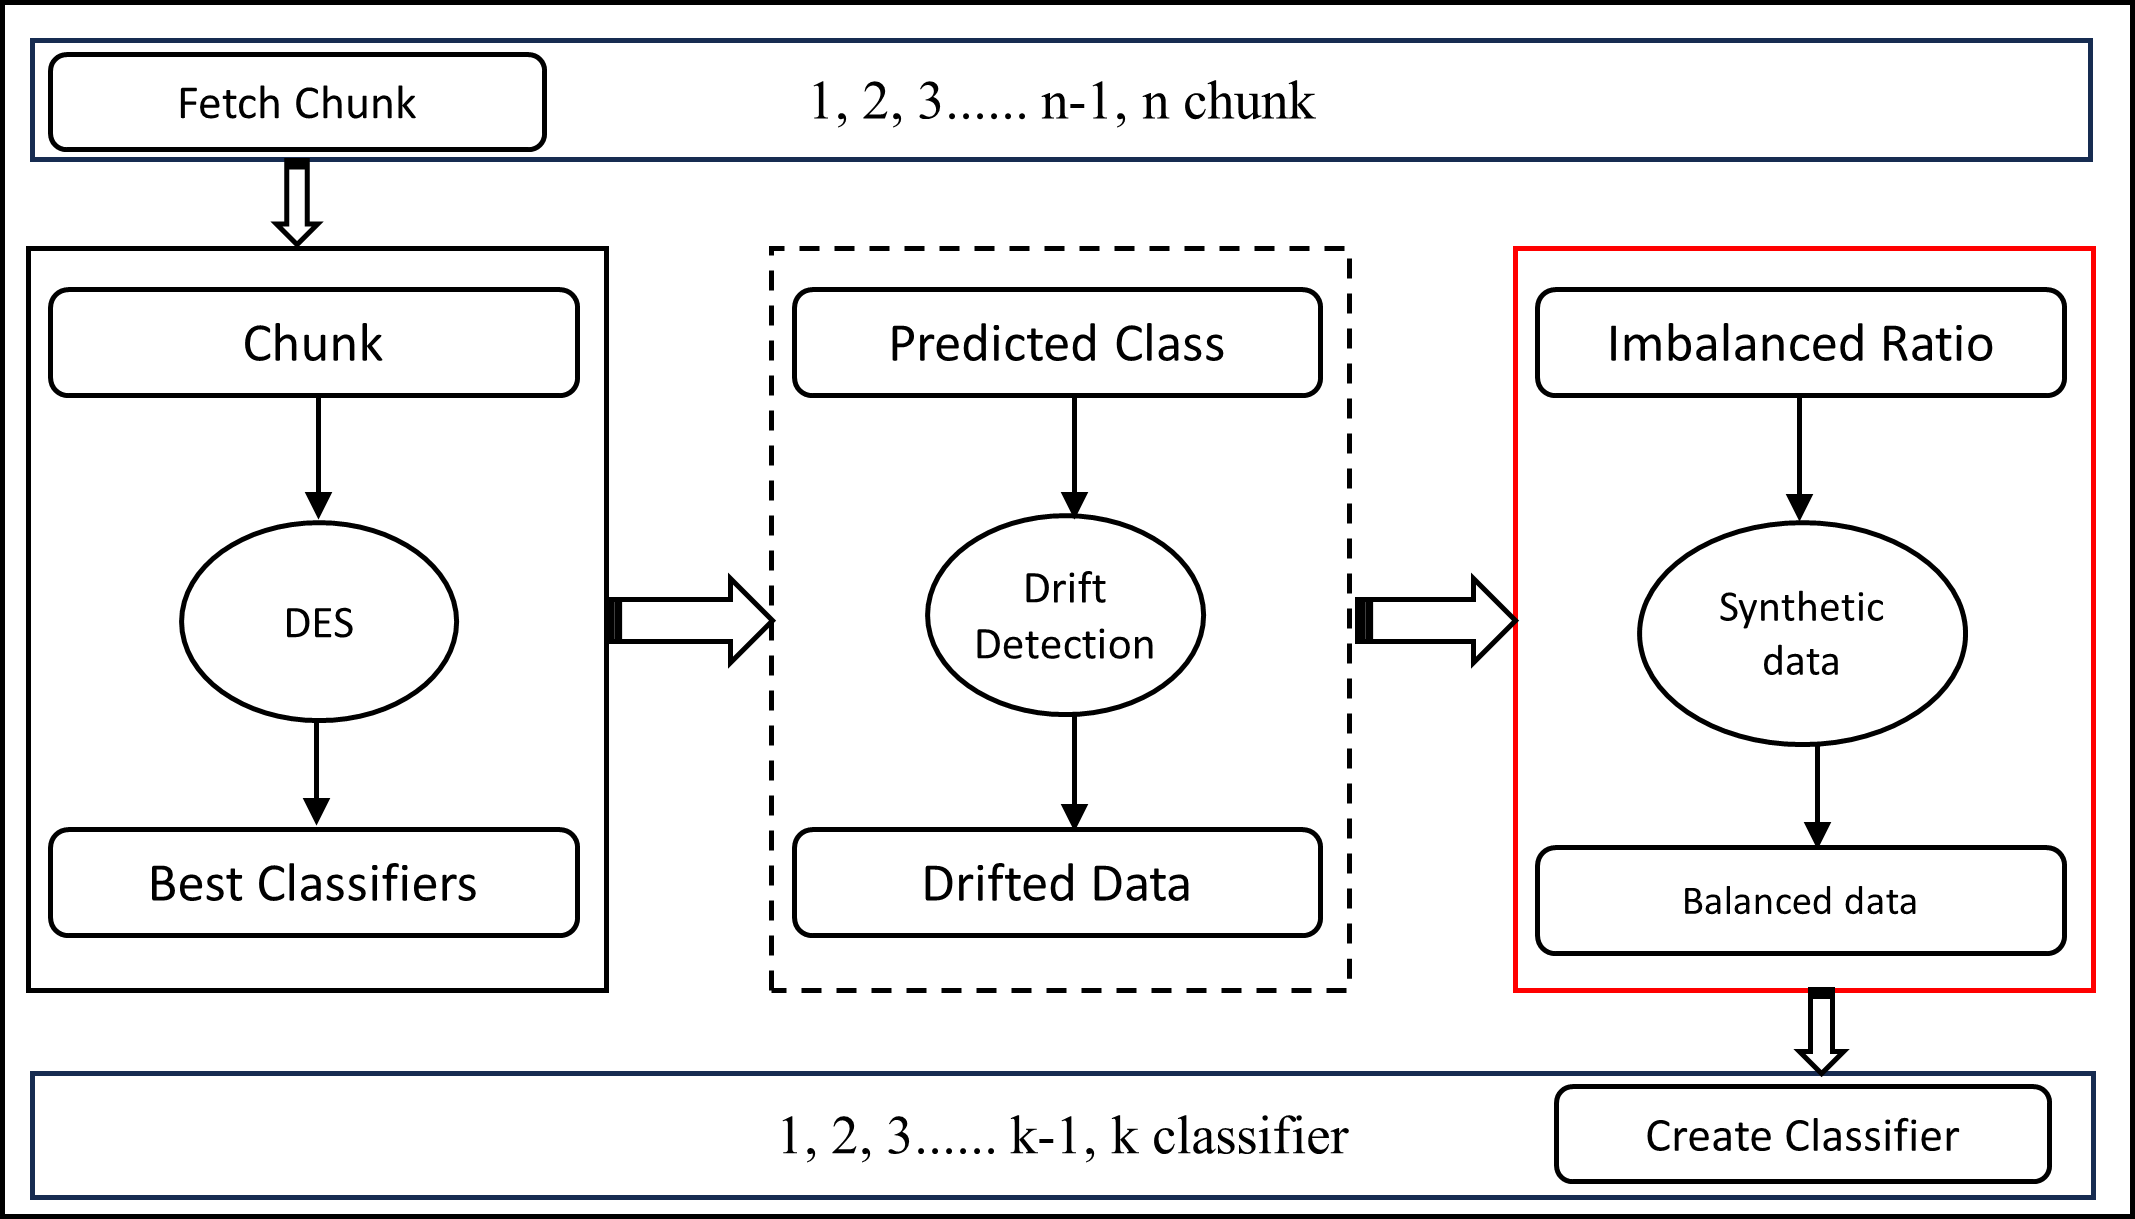
\includegraphics[width=1\linewidth]{4_Imbalanced/figures/approach_step_1.png}
	\caption{First Proposed Approach (PA1) for Imbalanced Multi-class Drifted Streams.}
	\label{fig:4_first_proposal_step_1}
\end{figure}
Specifically, as shown in Fig. \ref{fig:4_first_proposal_step_1}, the DES phase retrieves the current data chunk from the stream and applies the DES technique to select the most suitable classifiers for the received chunk. The selected classifiers were then passed to the second phase, where they were employed to predict the class of each instance within the received data chunk. Simultaneously, detectors like ADWIND or DDM are employed to monitor any occurrence of concept drift. If the discrepancy between the class frequency and standard deviation of the current chunk is significant, as described in reference \cite{gama2004learning}, and the imbalance ratio exceeds the average imbalance ratio, the current chunk is forwarded to the third phase, as indicated by the red rectangle in Fig. \ref{fig:4_first_proposal_step_1}. In the third phase, first proposed method uses a set of equations \ref{eq:4_first_proposal_1}\ref{eq:4_first_proposal_2}\ref{eq:4_first_proposal_3}
to identify minority classes. The initial equation computes the frequency of each class within the current chunk, where $i$ represents the current chunk, $c$ denotes the input class, and $y_i$ refers to the predicted class. The second equation determines the optimal frequency for each class based on the size of the chunk ($n$) and the number of classes in the current chunk($C$).

\begin{algorithm}[H]
	\caption{First Proposed Approach for Imbalanced Multi-class Streams.}
	\label{alg:4_alg_1}
	\KwIn{data stream, maximum classifiers pool size $\kappa$}
	\KwOut{Prediction $P$}
	\BlankLine
	$\psi, \Psi, \Omega, \mu \gets \emptyset$\;
	$\omega \gets 0$\;
	\For{stream have chunk}{
		\eIf{$a$ is the First chunk}{
			$k \gets$ \texttt{trainingNewClassifier}($a$)\;
			$P \gets$ \texttt{getPrediction}($a, k$)\;
		}{
			$k \gets$ \texttt{DES}($a, \Psi$)\;
			$P \gets$ \texttt{getPrediction}($a, k$)\;
			$\psi \gets$ \texttt{conceptDriftDetector}($P$)\;
			\If{$\psi > 0$}{
				$\Omega \gets$ get classes frequency according to Eq.1\;
				$\omega \gets$ best frequency according to Eq.2\;
				$\mu \gets$ get minority classes according to Eq.3\;
				$b \gets$ utilize $a$ and $\mu$ to get the synthetic data according to Algorithm \ref{alg:4_alg_2}\;
				trainingData $\gets a + b$\;
				$k \gets$ \texttt{trainingNewClassifier}(trainingData)\;
				$\Psi \gets \Psi + k$\;
				\If{$\Psi > \kappa$}{
					\texttt{removeWorstClassifier}($\Omega$)\;
				}
			}
			$P \gets$ \texttt{getPrediction}($a, k$)\;
		}
	}
	\Return{$P$}
	\end{algorithm}

Finally, the third equation identifies the classes as minority classes if their frequency deviates significantly from the standard deviation of the current chunk, where $sd_c$ represents the standard deviation of the class instances, and $frq_i$ refers to the standard deviation of the current chunk.
Figure \ref{fig:4_first_proposal_step_2} shows that phase These identified minority classes are then fed into the synthetic data generator phase, which increases the minority class samples to balance any imbalanced chunks. This ensures optimal performance for the new classifiers. Algorithm  \ref{alg:4_alg_1} provides a comprehensive outline of the process of the first proposed approach, which is the main contribution of this study and is designed to effectively address multiclass imbalanced and drifting data streams, uses streaming data as input, and systematically executes each step within the approach. The outcome of this process is the classification prediction generated using the first proposed approach.

\subsection{Synthetic Data Generator Phase Description}

Figure \ref{fig:4_first_proposal_step_2} presents a comprehensive overview of the synthetic data generator phase, which is an essential component responsible for generating synthetic samples by considering both data distribution and historical chunk behaviors. This phase has several advantages and can perform a wide range of tasks.
\begin{figure}[H]
	\centering
	
\includegraphics[width=1\linewidth]{4_Imbalanced/figures/approach_step_2.png}
	\caption{Flow Diagram of the Synthetic Data Generator.}
	\label{fig:4_first_proposal_step_2}
\end{figure}
\begin{itemize}
	\item \textbf{Similar chunk analysis:} Initially, the phase analyzes the current chunk distribution and identifies a similar chunk from historical data. This analysis forms the basis for generating synthetic samples that align with prevailing distribution patterns.
	\item \textbf{Oversampling method selection:} This phase utilizes the knowledge of the oversampling technique applied to the identified similar chunk. Consequently, it employs an alternative oversampling technique, using MLSMOTE and MLSOL, to create the most effective synthetic data. This step is designed not only to optimize the current classification but also to preemptively address potential drifts in similar future chunks.
	\item \textbf{Class overlap validation:} This step involves generating synthetic samples for the minority classes to effectively address the issue of minority classes and consequently enhance the classifier performance. The process utilizes the K-Nearest Neighbor (KNN) algorithm, as applied in \cite{lu2016concept}, to identify overlaps between newly generated data instances and existing instances. If overlaps are detected, the first proposed approach iteratively removes these samples because their presence can potentially diminish the overall classifier performance \cite{cruz2017meta, widmer1996learning}. Consequently, the first proposed approach generates alternative samples to address this challenge and preserve the primary objectives of the synthetic data generator step.
	\item \textbf{Continuous refinement:} This process iterates until it successfully generates high-quality synthetic data that aligns with the data distribution, minimizes overlap, and mitigates potential concept drift. The generated data were subsequently utilized in the training phase to improve classifier performance.
\end{itemize}
\begin{algorithm}[H]
	\caption{Synthetic Data Generator Algorithm.}
	\label{alg:4_alg_2}
	\KwIn{Minority classes $\mu$, current chunk $a$, sample size $\eta$, historical chunks $h$}
	\KwOut{Generated data $b$}
	$b \gets \emptyset$\;
	$f \gets \text{MLSMSOTE}$\;
	$knn \gets \text{kNearestNeighbor}(a)$\;
	$chunk \gets \text{similarChunk}(a, h)$\;
	$f \gets \text{similarChunkOverSamplingMethod}(chunk)$\;
	\If{$f = \text{MLSMSOTE}$}{
		$f \gets \text{MLSOL}$\;
	}
	\Else{
		$f \gets \text{MLSMSOTE}$\;
	}
	\While{$|b| < \eta$}{
		$p \gets \text{generateSyntheticPoint}(\mu, f)$\;
		$similarPointsClass \gets \text{KNN.getKneighbor}(b)$\;
		\If{$similarPointsClass = \mu$}{
			$b \gets b \cup \{p\}$\;
		}
	}
	\Return $b$\;
	\end{algorithm}
In Algorithm \ref{alg:4_alg_2}, also known as the Synthetic Data Generator, three essential elements are inputted: the minority class samples, the current data chunk, and the desired size for generating synthetic data. The primary objective of this algorithm is to produce synthetic data samples. To achieve this, the KNN algorithm is employed to identify any overlapping instances within the current chunk (Line 3). This algorithm utilizes two specific techniques, MLSMOTE \cite{gama2004learning} and MLSOL \cite{liu2017regional}. MLSMOTE was chosen for its introduction of randomness during instance generation, reducing its reliance on the local characteristics and distribution of the minority class. This randomization diminishes the likelihood of producing overlapping instances, particularly in cases where minority class instances are situated in overlapping regions. In contrast, MLSOL considers the local behavior of minority classes, resulting in synthetic points that closely resemble the minority class. This approach significantly improves the performance of the classifier (lines 4-10). Additionally, in this algorithm, specifically from lines 11 to 17, these lines are dedicated to generating synthetic instances that ensure non-overlap with existing classes. This procedure depends on the selected oversampling method and utilizes the KNN algorithm to guarantee that the generated instances do not overlap with the existing ones.


	\section{Mathematical Foundation for PA1}
	\label{sec:math_foundation_pa1}
	
	The mathematical foundation for PA1 involves key equations designed to identify and classify data chunks based on class frequencies and distributions. These equations are fundamental to analyzing imbalanced data streams effectively.
	
	Equation \ref{eq:4_first_proposal_1} calculates the frequency of a specific class \(c\) within a data chunk. For each instance \(y_i\), the frequency \(frq_{c}\) is incremented if the instance belongs to class \(c\):  
	\begin{equation}
	\label{eq:4_first_proposal_1}
	frq_{c} = \sum_{i=1}^{\text{chunk size}} 
	\begin{cases} 
	1, & \text{if } y_i = c \\
	0, & \text{otherwise}
	\end{cases}, \quad i = 1, 2, 3, \dots \text{chunk size}.
	\end{equation}
	
	Equation \ref{eq:4_first_proposal_2} defines the \textit{best frequency} for a chunk, \(freq_n\), as the proportion of instances \(n\) relative to the total number of classes \(C\):  
	\begin{equation}
	\label{eq:4_first_proposal_2}
	\text{best } freq_{n} = \frac{|n|}{|C|}.
	\end{equation}
	
	Finally, Equation \ref{eq:4_first_proposal_3} determines the type of each class in the chunk (\textit{Minority} or \textit{Majority}) by comparing the difference between the standard deviation (\(sd_c\)) and the class frequency (\(frq_i\)) against the best frequency of the chunk (\(freq_{\text{chunk}}\)):  
	\begin{equation}
	\label{eq:4_first_proposal_3}
	\text{classes type}_{\text{chunk}} = \sum_{c=1}^{C} 
	\begin{cases} 
	\text{Minority,} & \text{if } diff(sd_c - frq_i) > \text{best } freq_{\text{chunk}} \\
	\text{Majority,} & \text{otherwise}.
	\end{cases}
	\end{equation}
	
	These equations collectively enable precise identification of class types within data chunks, forming a critical component of the PA1 framework.
	
	
%%%%%%%%%%%%%%%%%%%%%%%%%%%%%%%%%%%%%%%%%%%%%%%
%
%   Families of Traffic Forecasting Problems
%
%%%%%%%%%%%%%%%%%%%%%%%%%%%%%%%%%%%%%%%%%%%%%%%

%\usepackage{cite}
%\usepackage{multirow}
%\usepackage{rotating} 
%\usepackage[table,xcdraw]{xcolor}
%\usepackage{float}
%\usepackage[utf8]{inputenc}
%\usepackage{amsmath,amssymb,amsfonts}
%\usepackage{algorithmic}
%\usepackage{graphicx}
%\usepackage{textcomp}
%\usepackage{rotating}
%\usepackage{verbatim}


\section{Experimental Results}
\label{sec:4_5_Expsetup}

The objective of the experiments conducted in this study was to evaluate the efficacy of multiclass oversampling techniques in enhancing the performance of the proposed method in imbalanced drifted multiclass classification streams. Our primary goal was to develop a novel approach that combines Dynamic Ensemble Selection (DES) to improve classification accuracy and robustness in such streams. These experiments yielded valuable insights that could further refine the performance of the proposed approach and its ability to effectively handle imbalanced data streams. These findings provide a better understanding of the capabilities of the proposed approach and offer insights into an optimal strategy for tackling minority class issues and concept drift in imbalanced data streams. This study contributes to the advancement of stream mining techniques for generating more accurate and robust classification models in dynamic data stream environments. By addressing the challenges posed by minority classes and concept drift, this study offers valuable insights for improving the performance of the proposed approach and enhancing the overall efficiency of stream mining. The two main questions to be answered are:

\begin{itemize}
  % \setlength{\itemindent}{-.5in}
  
      \item $\pmb{Q_1}$: What is the impact of reduced and consistent data on the performance of ensemble learning?
      \item  $\pmb{Q_2}$: Is it possible with the search capability of swarm intelligence to enhance the combination of classifiers? 
  \end{itemize}

\subsection{Experimental setup}
The evaluation of the proposed method incorporated the utilization of various metrics such as recall, precision, specificity, f1 score, balanced accuracy score (BAC), and geometric mean score (G-mean) \cite{bu2016pdf}. The experimental protocol utilized for evaluation was the test-then-train approach \cite{venkatasubramanianinformation}, where the classification classifier was trained on a specific data chunk and subsequently evaluated on the subsequent one. The chunk size was standardized for all utilized data streams to 2,000 instances. We employed four classification classifiers as base estimators: K-Nearest Neighbor (KNN), Support Vector Machine (SVM), Gaussian Naive Bayes (GNB), and Hoeffding Tree (HT), as implemented in scikit-learn \cite{frias2014online}. A pool of classifiers was constructed with a maximum size of L = 8, where the DES selected the best classifier for each chunk. If the pool surpassed the set threshold (L), the classifier with the lowest performance was eliminated. The experiments were conducted using Python programming language, and the source code was publicly available on GitHub\footnote{\url{https://github.com/Amadkour/dynamic__classification_ensembles_for_handling_imbalanced_multi-class_drifted_data_streams.git}} . We conducted a comparison between multiclass oversampling techniques (MLSMOTE and MLSOL) and our proposed approach to demonstrate the effectiveness of our contribution. Additionally, we conducted these experiments using two different concept drift detectors, ADWIN \cite{storkey2008training} and DDM \cite{losing2016knn}, to demonstrate the adaptability and robustness of our proposed approach across varying drift detectors.

\subsection{Data Streams}
In this study, the proposed approach was assessed using various datasets including benchmark datasets, a real application stream dataset, and synthetic data streams. The Stream-learn Python library was used to conduct the evaluations \cite{dries2009adaptive}. Table \ref{tab:4_first_proposal_result_table_1} illustrates the benchmark dataset employed in this study, which consists of the Covertype dataset containing 40 features, seven classes, and 581,010 instances. For real application stream evaluation, the Sensor stream dataset was used, which consisted of five features, 58 classes, and 392,600 instances. This represents a real-world application scenario and provides valuable insights into the performance of the proposed approach in practical settings. Synthetic datasets were generated using Scikit-learn Python library to evaluate the performance of the proposed approach. The synthetic dataset was designed to simulate data streams and comprised 10 features and four classes divided into 200 chunks of 2,000 instances each. The performance of the proposed approach was systematically evaluated using these datasets and a stream-learn library. These evaluations provided insights into the effectiveness of the proposed approach in handling different types of data streams, including benchmark datasets, real application streams, and synthetic data streams.

\begin{table}[h!]
  \centering
  \resizebox{\textwidth}{!}{
  \begin{tabular}{|l|c|c|c|}
  \hline
  \textbf{Dataset} & \textbf{Number of Features} & \textbf{Number of Classes} & \textbf{Number of Instances} \\ \hline
  Covertype dataset\footnote{\url{http://archive.ics.uci.edu/dataset/31/covertype}} & 40 & 7 & 581,010 \\ \hline
  Sensor Stream dataset\footnote{\url{https://www.cse.fau.edu/~xqzhu/Stream/sensor.arff}} & 5 & 58 & 392,600 \\ \hline
  Synthetic stream & 8 & 3 & 200,000 \\ \hline
  \end{tabular}
  }
  \caption{Characteristics of the datasets used in the experiments.}
  \label{tab:4_first_proposal_result_table_1}
  \end{table}

\subsection{Analysis of Experimental Results}
The performance of the proposed framework was comprehensively assessed on multiple data streams, considering two distinct concept drift detectors, ADWIN and DDM. To ensure thorough evaluation, six key performance metrics—F1 score, recall, precision, G-mean, specificity, and balanced accuracy—were carefully presented using two visualization diagrams: radar and line. A radar diagram was strategically utilized to provide an overview that effectively depicted the performance of each algorithm across the six metrics. The mean value of each metric was calculated to present the overall performance of each method (MLSMOTE, MLSOL, PA). It is important to note that the PA is represented by red lines.
\subsubsection{Results on the Benchmark Stream}
The results of the mentioned methods (MLSMOTE, MLSOL, PA) applied to the Covertype dataset are presented in Fig. \ref{fig:4_first_proposal_result_exp_1}
, utilizing ADWIN as the drift detector. The radar diagram shows that the metric values were between 0.8 and 1.0. MLSOL exhibited the highest precision, whereas MLSOTE and PA had nearly identical values. However, PA excels in other metrics, whereas MLSMOTE has the lowest values. The line diagram in Fig. \ref{fig:4_first_proposal_result_exp_1}
shows the classification accuracy across 100 data chunks using the specificity metric for the methods in each chunk. Notably, all methods exhibit suboptimal accuracy during the first 20 chunks. However, a noticeable improvement was observed beyond this initial phase. The key factor driving this improvement was the expansion of the classifier pool, which now encompasses a growing number of classifiers. This expansion enables the Dynamic Ensemble Selection (DES) technique to become more proficient in selecting the most suitable classifier for each incoming chunk. Consequently, accuracy experienced a significant boost in later chunks, reflecting the adaptability and effectiveness of the ensemble approach. From chunk 20 to the last chunk, PA achieved the highest accuracy, whereas MLSMOTE recorded the lowest accuracy. PA's superior performance of the PA is credited to its use of historical chunks to generate optimal nonoverlapping samples, thereby effectively training the pool classifiers. In Fig. \ref{fig:4_first_proposal_result_exp_2}
, the same dataset is employed with the DDM functioning as the drift detector. The radar plot illustrates results comparable to those of the prior experiment, whereas the line diagram underscores PA's supremacy in most chunks. However, it also reveals that all approaches demonstrate diminished performance, in contrast to Fig. \ref{fig:4_first_proposal_result_exp_1} (ADWIN), suggesting that ADWIN surpasses DDM when utilized in the Covertype data stream.


\begin{figure}[!ht]
	\centering
	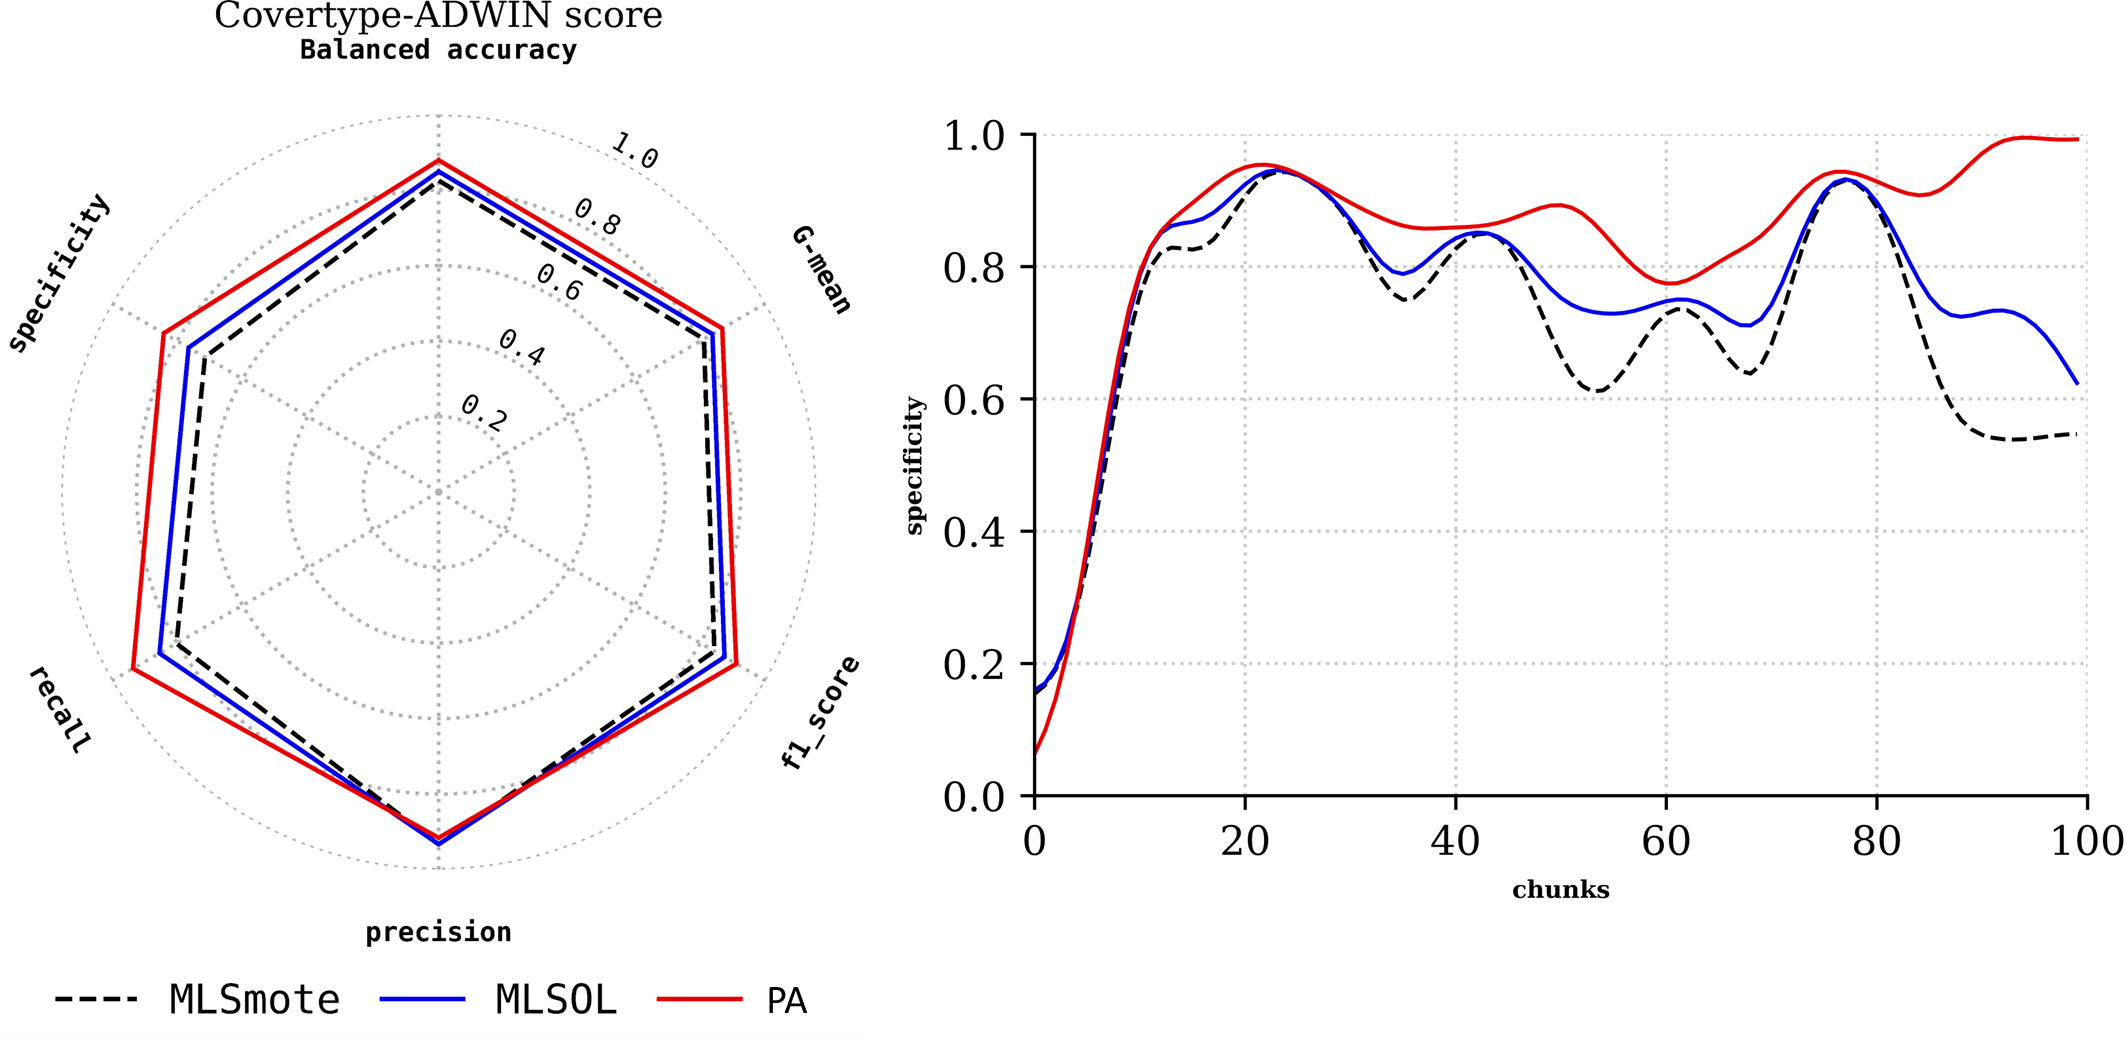
\includegraphics[width=1\linewidth]{4_Imbalanced/figures/exp_1.png}
	\caption{Performance of the Proposed Approach (PA), MLSMOTE, and MLSOL techniques on the Covertype Benchmark dataset using the ADWIN concept drift detector.}
	\label{fig:4_first_proposal_result_exp_1}
\end{figure}

\begin{figure}[!ht]
	\centering
	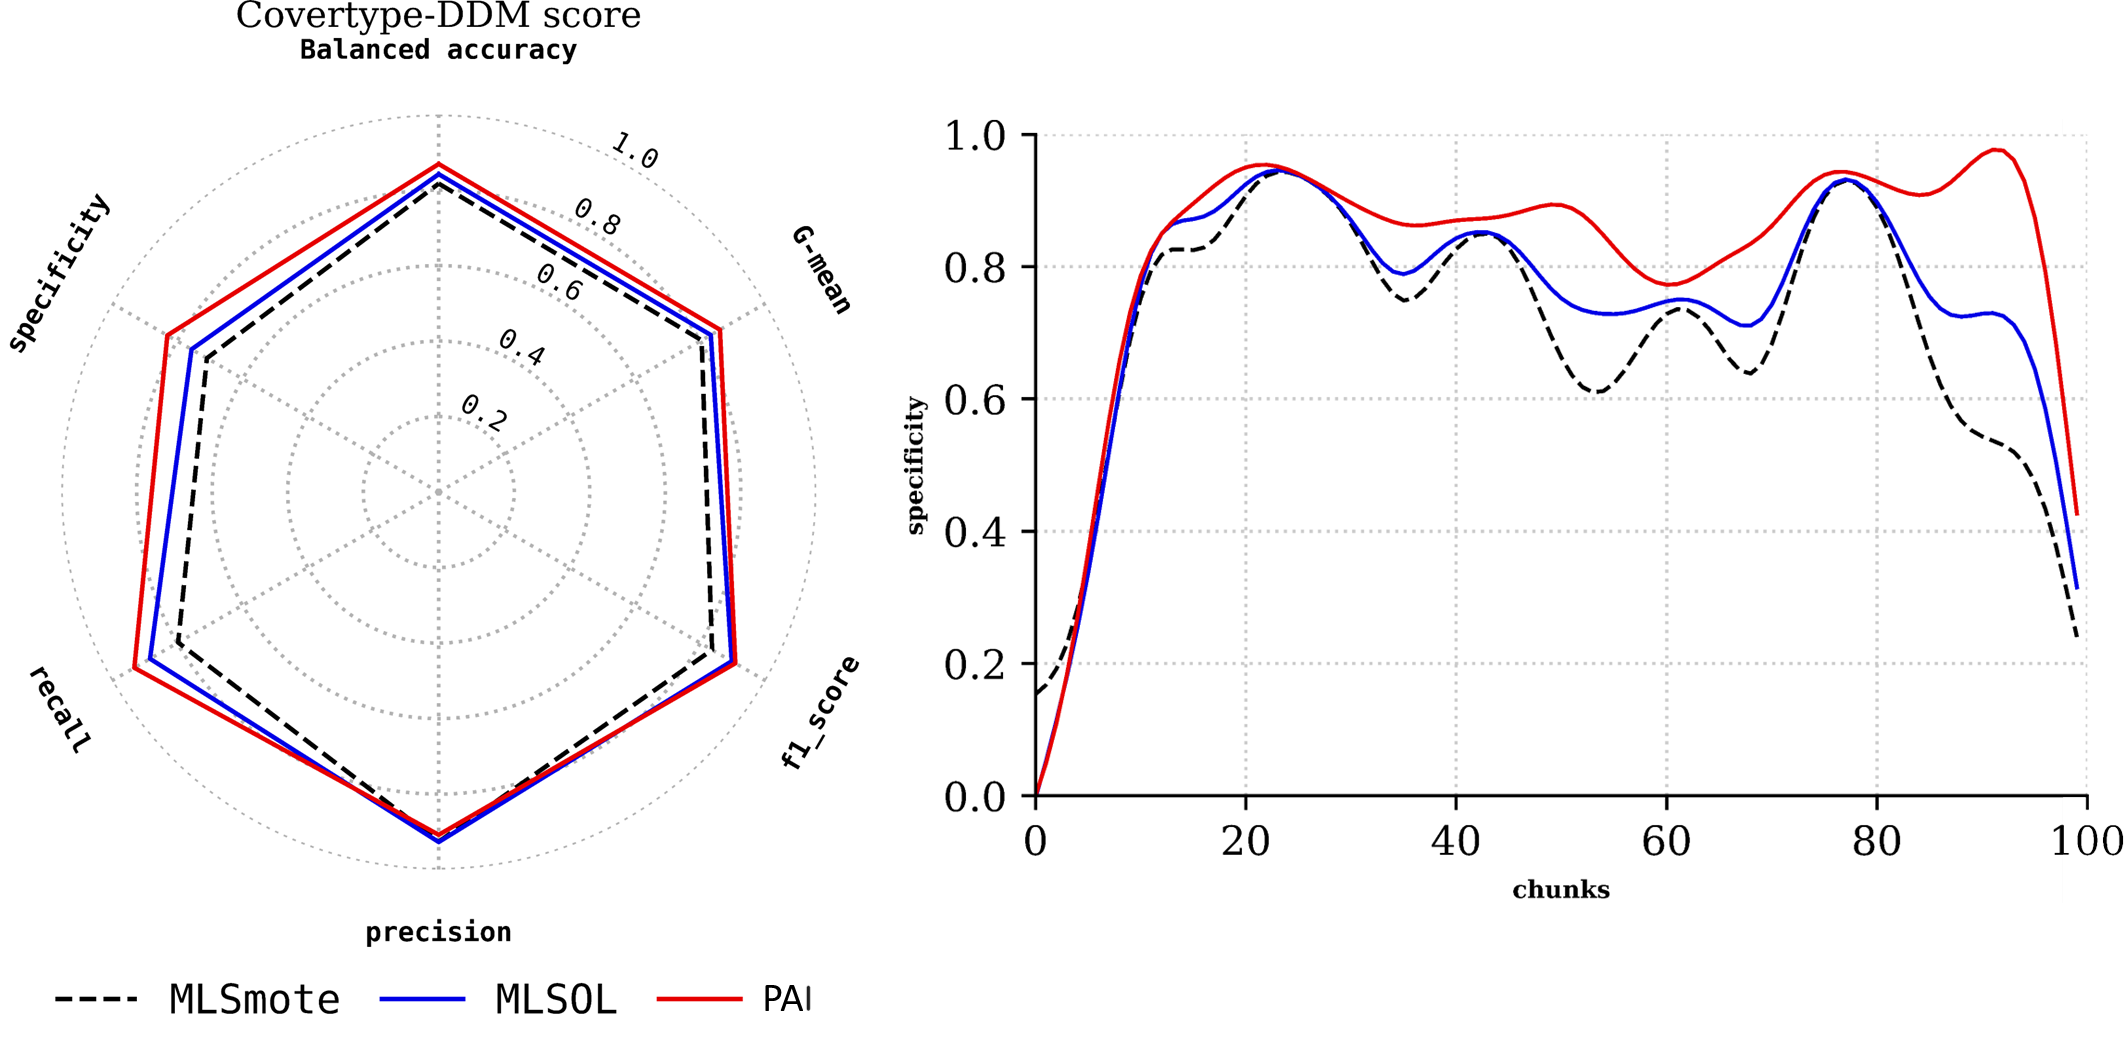
\includegraphics[width=1\linewidth]{4_Imbalanced/figures/exp_2.png}
  \caption{Performance of the Proposed Approach (PA), MLSMOTE, and MLSOL techniques on the Covertype Benchmark stream using the DDM concept drift detector.}
	\label{fig:4_first_proposal_result_exp_2}
\end{figure}

\subsubsection{Results on the Real Application Stream}
Fig. \ref{fig:4_first_proposal_result_exp_3} illustrates the outcomes of employing the three methods on the Sensor data stream using ADWIN as the drift detector. The radar graph depicts metric values ranging from 0.6 to 0.8, which indicate the pronounced drift and imbalance of the Sensor stream. In terms of the precision and recall metrics, the three methods exhibited almost identical values, whereas PA stood out in the other metrics. In contrast, MLSMOTE and MLSOL displayed similar values. By examining the line graph in Fig. \ref{fig:4_first_proposal_result_exp_3}
, it is evident that during the initial 30 chunks, PA's performance of PA might be suboptimal in some instances because of the limited number of classifiers in the pool. However, after the first 30 chunks, the performance significantly improved with the addition of more classifiers. In the same graph, PA consistently achieved the highest performance across all chunks, whereas MLSMOTE exhibited lower performance in certain chunks, and MLSOL exhibited lower performance in the other chunks. In Fig. \ref{fig:4_first_proposal_result_exp_4}, using the same dataset with the DDM as the drift detector, the radar plot metrics indicate lower results compared to the previous experiment. Nonetheless, the line graph underscores PA's dominance of PA in most chunks, although all methods exhibit nearly identical performance across the entire set of chunks. Overall, the performance of all the methods in Fig. \ref{fig:4_first_proposal_result_exp_4} is inferior to that in Fig. \ref{fig:4_first_proposal_result_exp_3} (ADWIN), which highlights ADWIN's superiority of ADWIN over DDM when applied to the Sensor data stream. 


\begin{figure}[!ht]
	\centering
	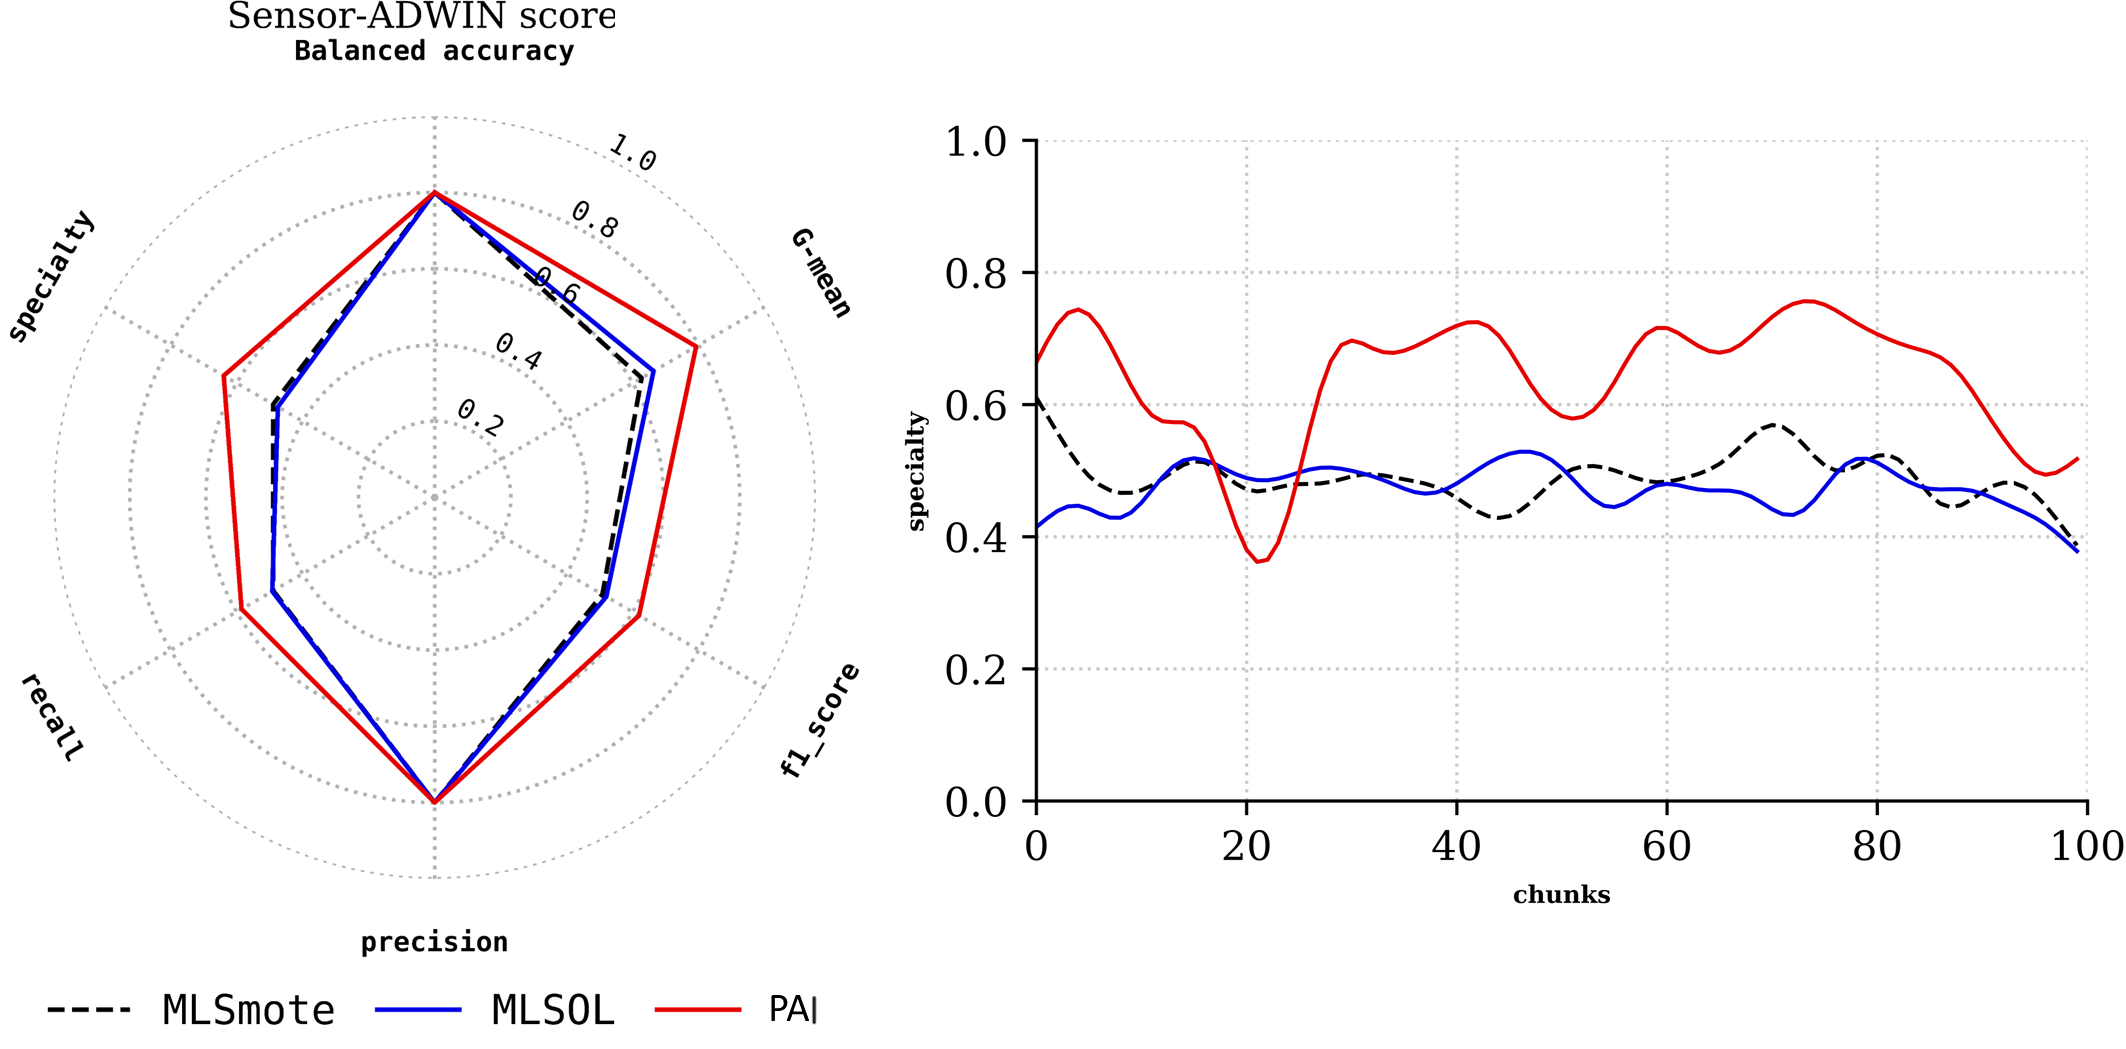
\includegraphics[width=1\linewidth]{4_Imbalanced/figures/exp_3.png}
  \caption{Performance of the Proposed Approach (PA), MLSMOTE, and MLSOL techniques on the Sensor real application stream using the ADWIN concept drift detector.}
	\label{fig:4_first_proposal_result_exp_3}
\end{figure}

\begin{figure}[!ht]
	\centering
	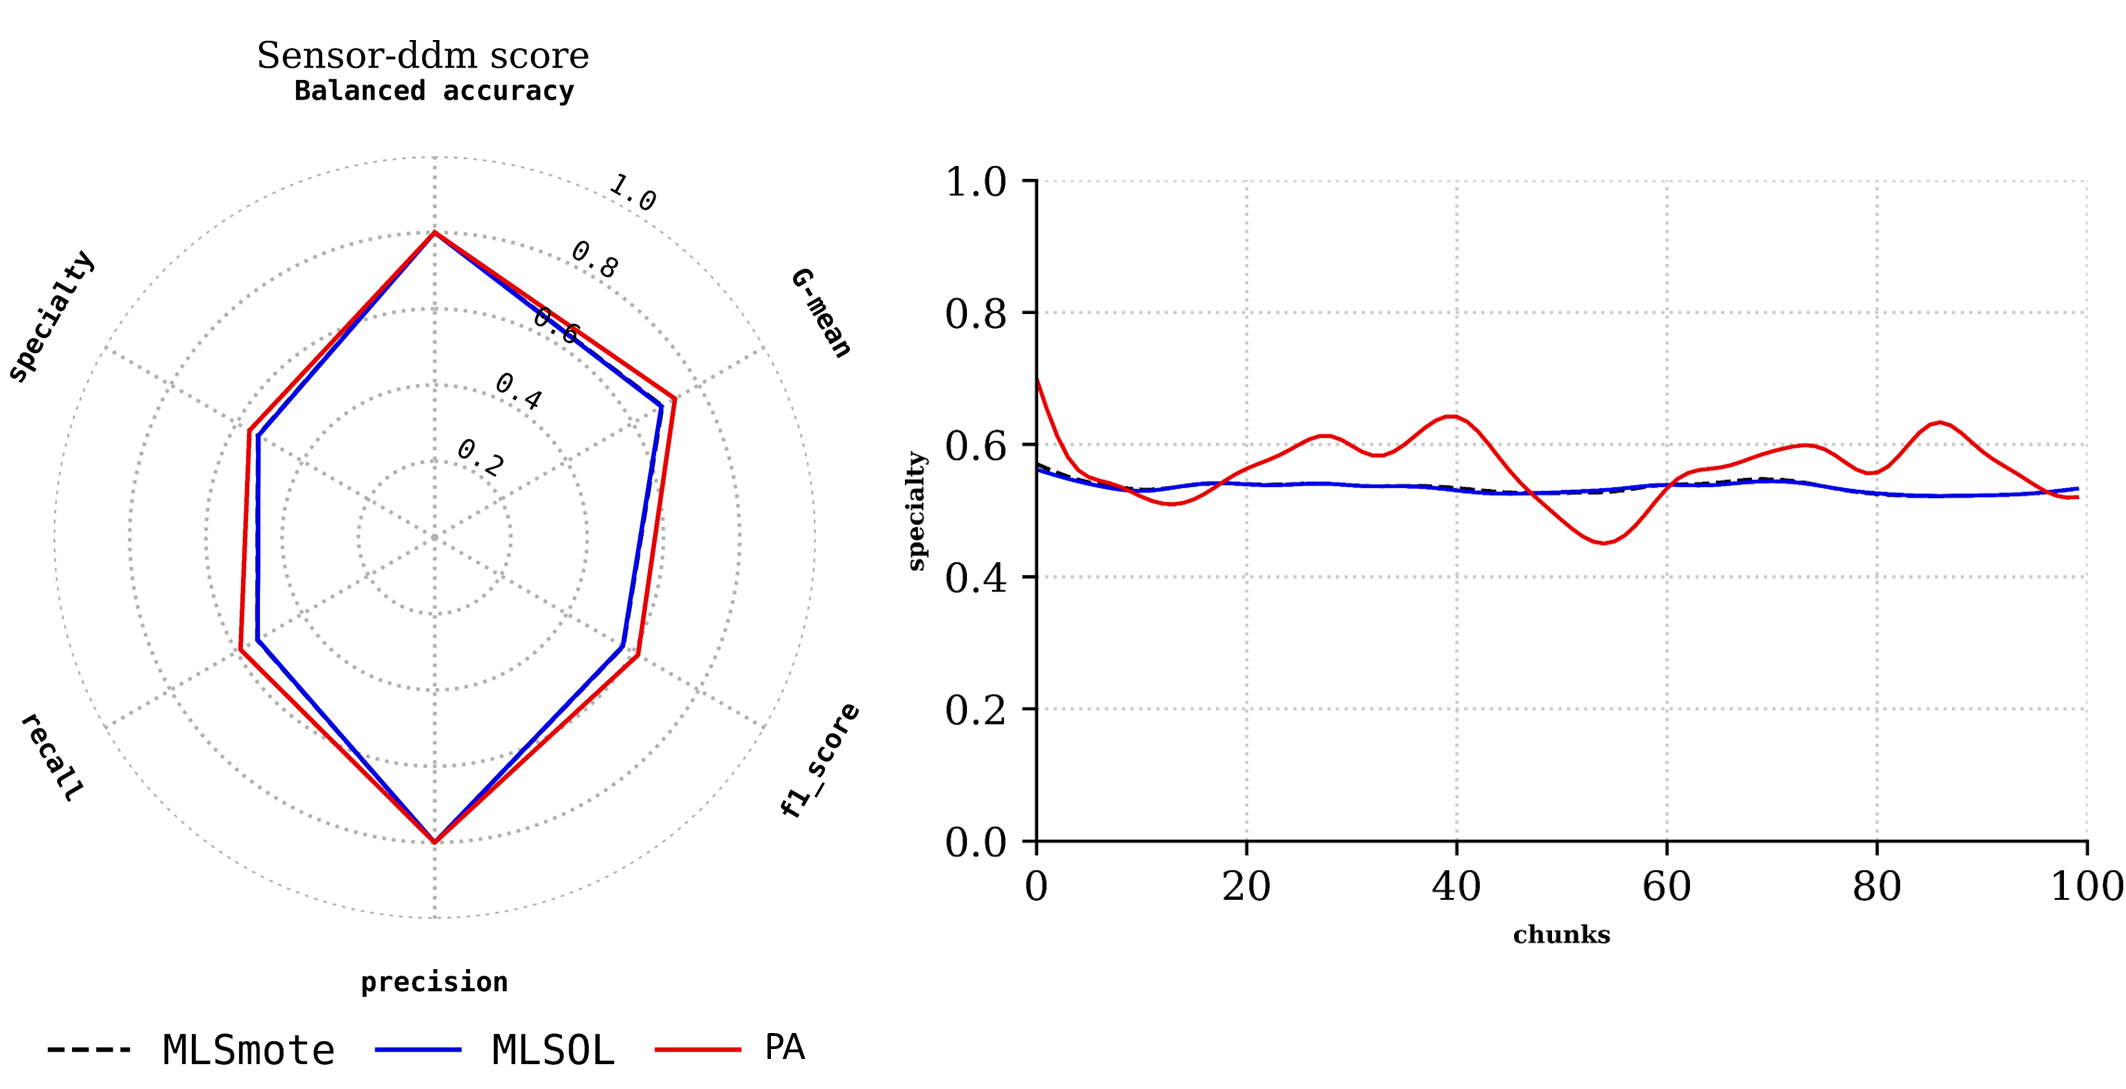
\includegraphics[width=1\linewidth]{4_Imbalanced/figures/exp_4.png}
  \caption{Performance of the Proposed Approach (PA), MLSMOTE, and MLSOL techniques on the Sensor real application stream using the DDM concept drift detector.}
	\label{fig:4_first_proposal_result_exp_4}
\end{figure}


\subsubsection{Results on the Synthetic Stream}
The results of applying the same methods on the synthetic data stream using ADWIN as the drift detector are presented in Fig. \ref{fig:4_first_proposal_result_exp_5}. The radar diagram indicates metric values ranging from 0.6 to 0.8, suggesting that the synthetic stream is prone to frequent drifts. While MLSOL exhibited the highest precision, MLSOTE exhibited the lowest values. Conversely, PA performed well in other metrics, and MLSMOTE demonstrated the least favorable values. Upon examining the line diagram in Fig. \ref{fig:4_first_proposal_result_exp_5}, it becomes evident that during the initial ten chunks, the PA's performance might be suboptimal because of the limited number of classifiers in the pool. However, after the first ten chunks, the performance improved significantly with the inclusion of more classifiers. In the same diagram, PA consistently achieves the highest performance across all chunks, whereas MLSOL maintains satisfactory performance, and MLSMOTE exhibits lower performance throughout. In Fig. \ref{fig:4_first_proposal_result_exp_6}, using the same synthetic data stream but with the DDM as the drift detector, the radar plot metrics produce similar results to the previous experiment. However, the line diagram emphasizes the same outcomes as those in the previous experiment. Nevertheless, MLSOL and MLSMOTE achieved lower values than the previous experiment. These findings confirmed ADWIN's superiority of ADWIN over DDM when applied to synthetic data streams. These results highlight the versatility and robustness of the algorithm, demonstrating its effectiveness in handling concept drift across diverse datasets, including the challenging synthetic dataset, Covertype dataset, and Sensor dataset, regardless of whether ADWIN or DDM is used as the concept drift detector.

\begin{figure}[!ht]
	\centering
	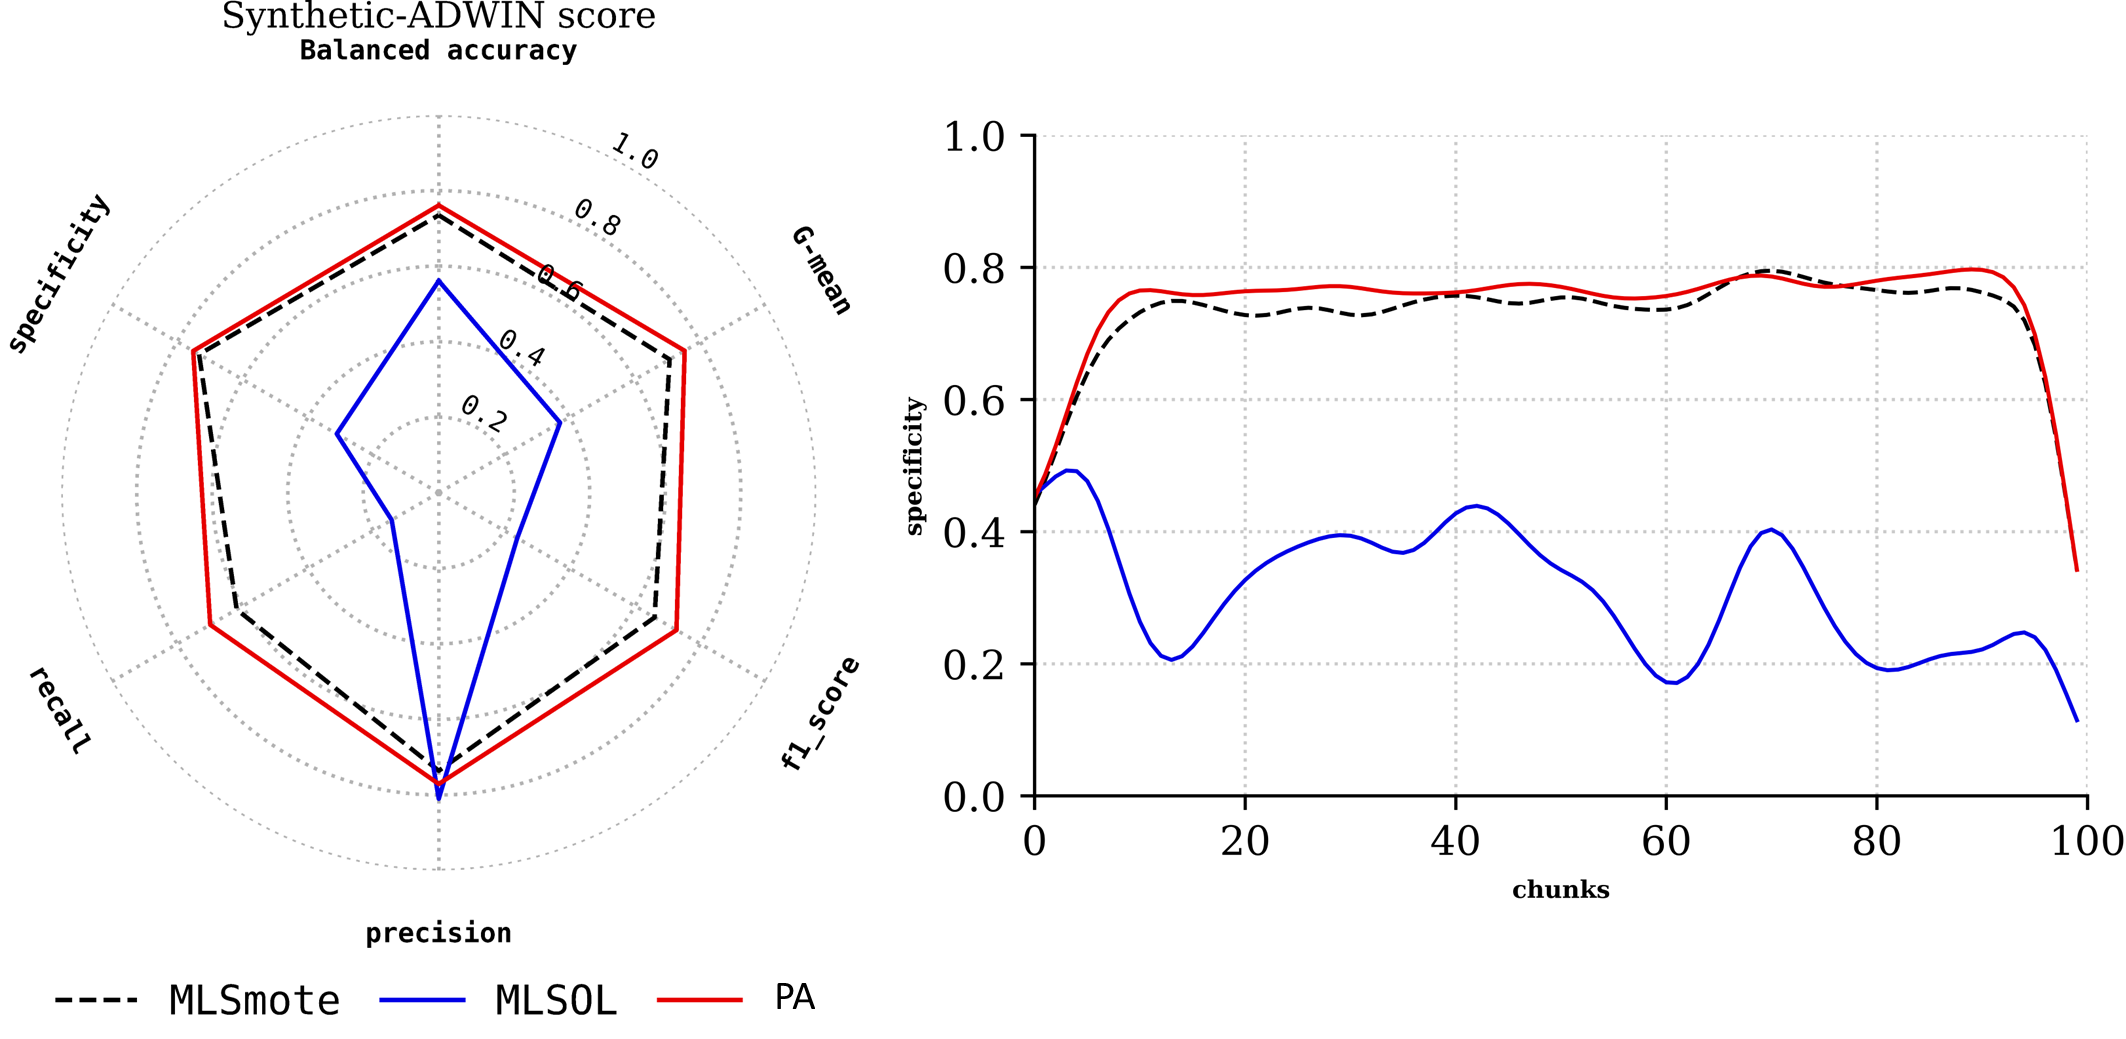
\includegraphics[width=1\linewidth]{4_Imbalanced/figures/exp_5.png}
  \caption{Performance of the Proposed Approach (PA), MLSMOTE, and MLSOL techniques on the Synthetic stream using the ADWIN concept drift detector.}
	\label{fig:4_first_proposal_result_exp_5}
\end{figure}

\begin{figure}[!ht]
	\centering
	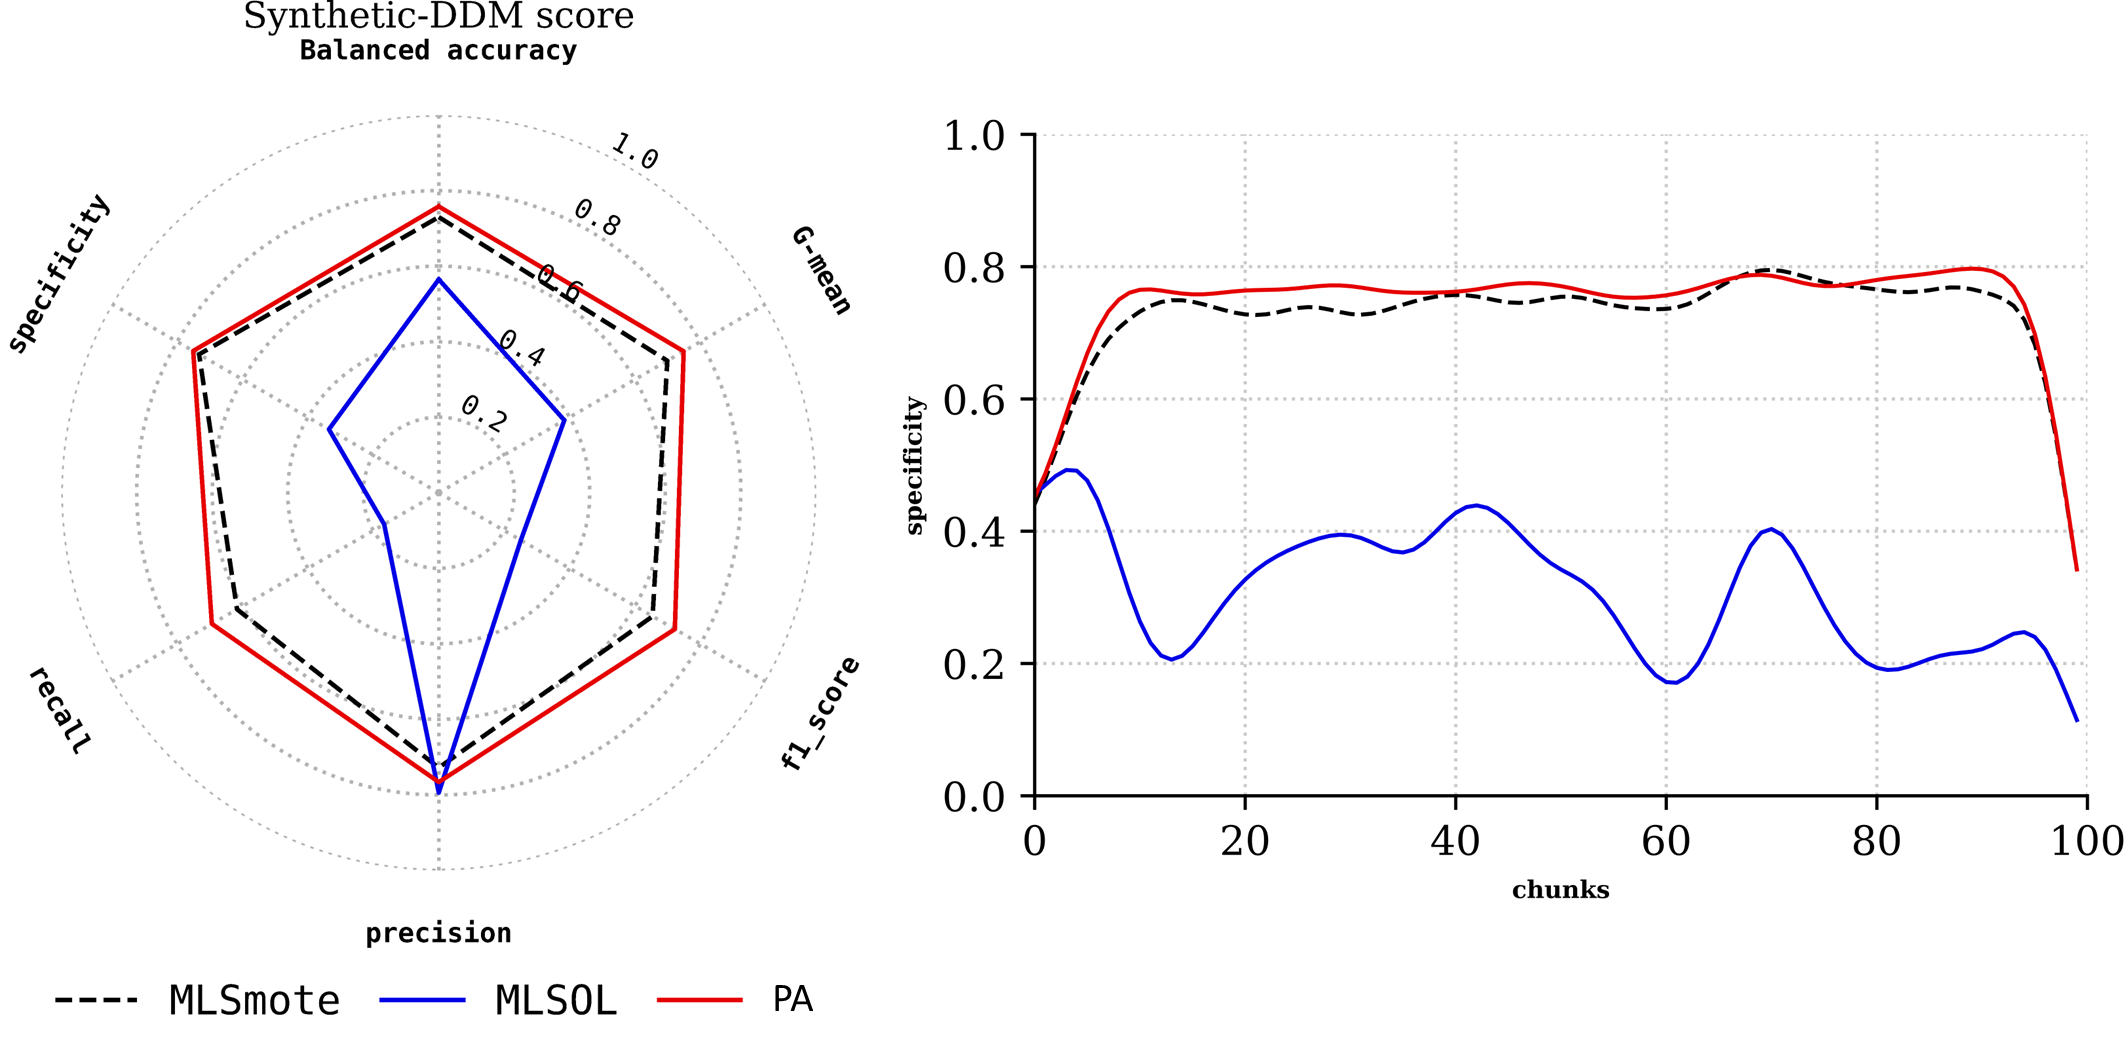
\includegraphics[width=1\linewidth]{4_Imbalanced/figures/exp_6.png}
  \caption{Performance of the Proposed Approach (PA), MLSMOTE, and MLSOL techniques on the Synthetic stream using the DDM concept drift detector.}
	\label{fig:4_first_proposal_result_exp_6}
\end{figure}


\subsection{Analysis of Class Overlap Factor between Proposed Approach (PA), MLSMOTE, and MLSOL Techniques.}
In our experimental study, we aimed to identify the critical factors that influence the selection of an optimal approach for minority classes in imbalanced drifted streams. These factors include various aspects, such as dataset characteristics, the choice of concept drift detectors, and the effectiveness of the algorithm in handling class overlap. To compare the overlapping class behavior of our proposed approach (PA) with MLSMOTE and MLSOL, we systematically designed experiments organized into groups of ten chunks. The results were visualized in bar diagrams, contrasting PA with other methods (MLSMOTE and MLSOL). Figures \ref{fig:4_first_proposal_result_exp_7, fig:4_first_proposal_result_exp_8, fig:4_first_proposal_result_exp_9} present ten groups, each with three bars representing MLSOTE, MLSOL, and PA, respectively. Each bar visually represents overlapped samples for ten chunks of several data streams, considering distinct concept drift detectors, specifically ADWIN and DDM.
Fig. \ref{fig:4_first_proposal_result_exp_7} shows two diagrams for the ADWIN and DDM detectors. In the ADWIN diagram, the third bar group (chunks 20-30) lacks overlapping samples because this chunk range does not have drifts, and no synthetic samples are generated for the training step. The sixth and tenth groups have the highest overlapped samples because these groups experience many drifts, leading to the generation of several samples and, consequently, the data indicates that MLSMOTE displays the highest number of overlapping samples across all groups, while PA exhibits very few, except for the last group (90-100), which has a small number of overlapping samples. However, the DDM diagram has more overlapping samples than the ADWIN diagram because the DDM detector detects fewer drifts than ADWIN. Specifically, the last value on the Y-axis of the ADWIN diagram is 3,000 samples, while the last value on the Y-axis of the DDM diagram is 2,000 samples. Fig. \ref{fig:4_first_proposal_result_exp_8} and Fig. \ref{fig:4_first_proposal_result_exp_9} display the overlapping samples of the three methods on the Sensor and synthetic data streams, respectively. In Fig. \ref{fig:4_first_proposal_result_exp_8}, the ADWIN diagram demonstrates fewer overlapped samples than in Fig. \ref{fig:4_first_proposal_result_exp_8}, indicating a lower number of drifts in the Sensor stream. The overall diagram indicates that our proposed approach achieves fewer overlapped samples than MLSOL and MLSMOTE, with MLSMOTE having the highest number of overlapped samples. In the DDM diagram of Fig. 10, the number of overlapped samples is lower than in Fig. \ref{fig:4_first_proposal_result_exp_7}, with our proposed approach consistently achieving the lowest number of overlapped samples across most group bars.
In Fig. \ref{fig:4_first_proposal_result_exp_9}, the ADWIN and DDM diagrams exhibit the greatest number of overlapped samples compared to the earlier figures. This suggests that the synthetic stream underwent frequent drifts and was more susceptible to noise. Consequently, the last value on the Y-axis in both the ADWIN and DDM diagrams was recorded for 7,000 samples. Our proposed approach consistently achieves the lowest number of overlapped samples, whereas MLSMOTE consistently attains the highest number of overlapped samples across most group bars in both the ADWIN and DDM diagrams. In conclusion, our thorough examination of overlapping class instances across MLSMOTE, MLSOL, and our proposed approach consistently reveals minimal overlapped samples compared to other methods, regardless of whether DDM or ADWIN is employed as drift detectors

\begin{figure}[!ht]
	\centering
	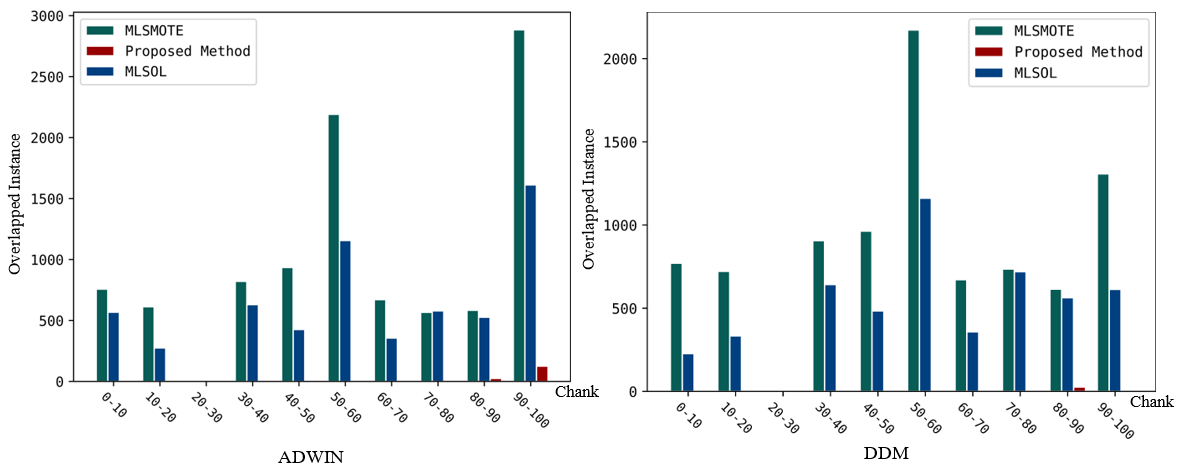
\includegraphics[width=1\linewidth]{4_Imbalanced/figures/exp_7.png}
  \caption{Overlapping generated points of the Proposed Approach (PA), MLSMOTE, and MLSOL techniques on the Covertype benchmark stream.}
	\label{fig:4_first_proposal_result_exp_7}
\end{figure}

\begin{figure}[!ht]
	\centering
	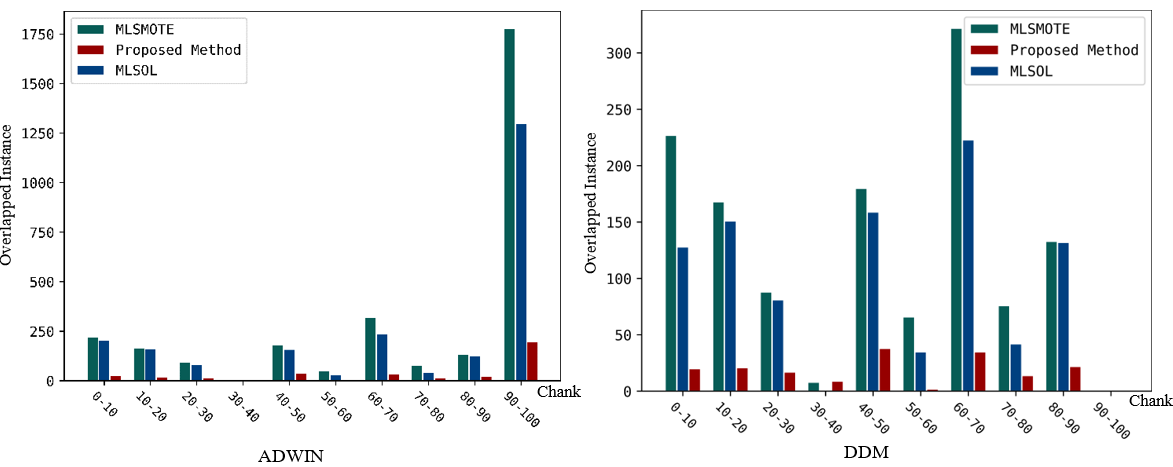
\includegraphics[width=1\linewidth]{4_Imbalanced/figures/exp_8.png}
  \caption{Overlapping generated points of the Proposed Approach (PA), MLSMOTE, and MLSOL techniques on the Sensor real application stream.}
	\label{fig:4_first_proposal_result_exp_8}
\end{figure}

\begin{figure}[!ht]
	\centering
	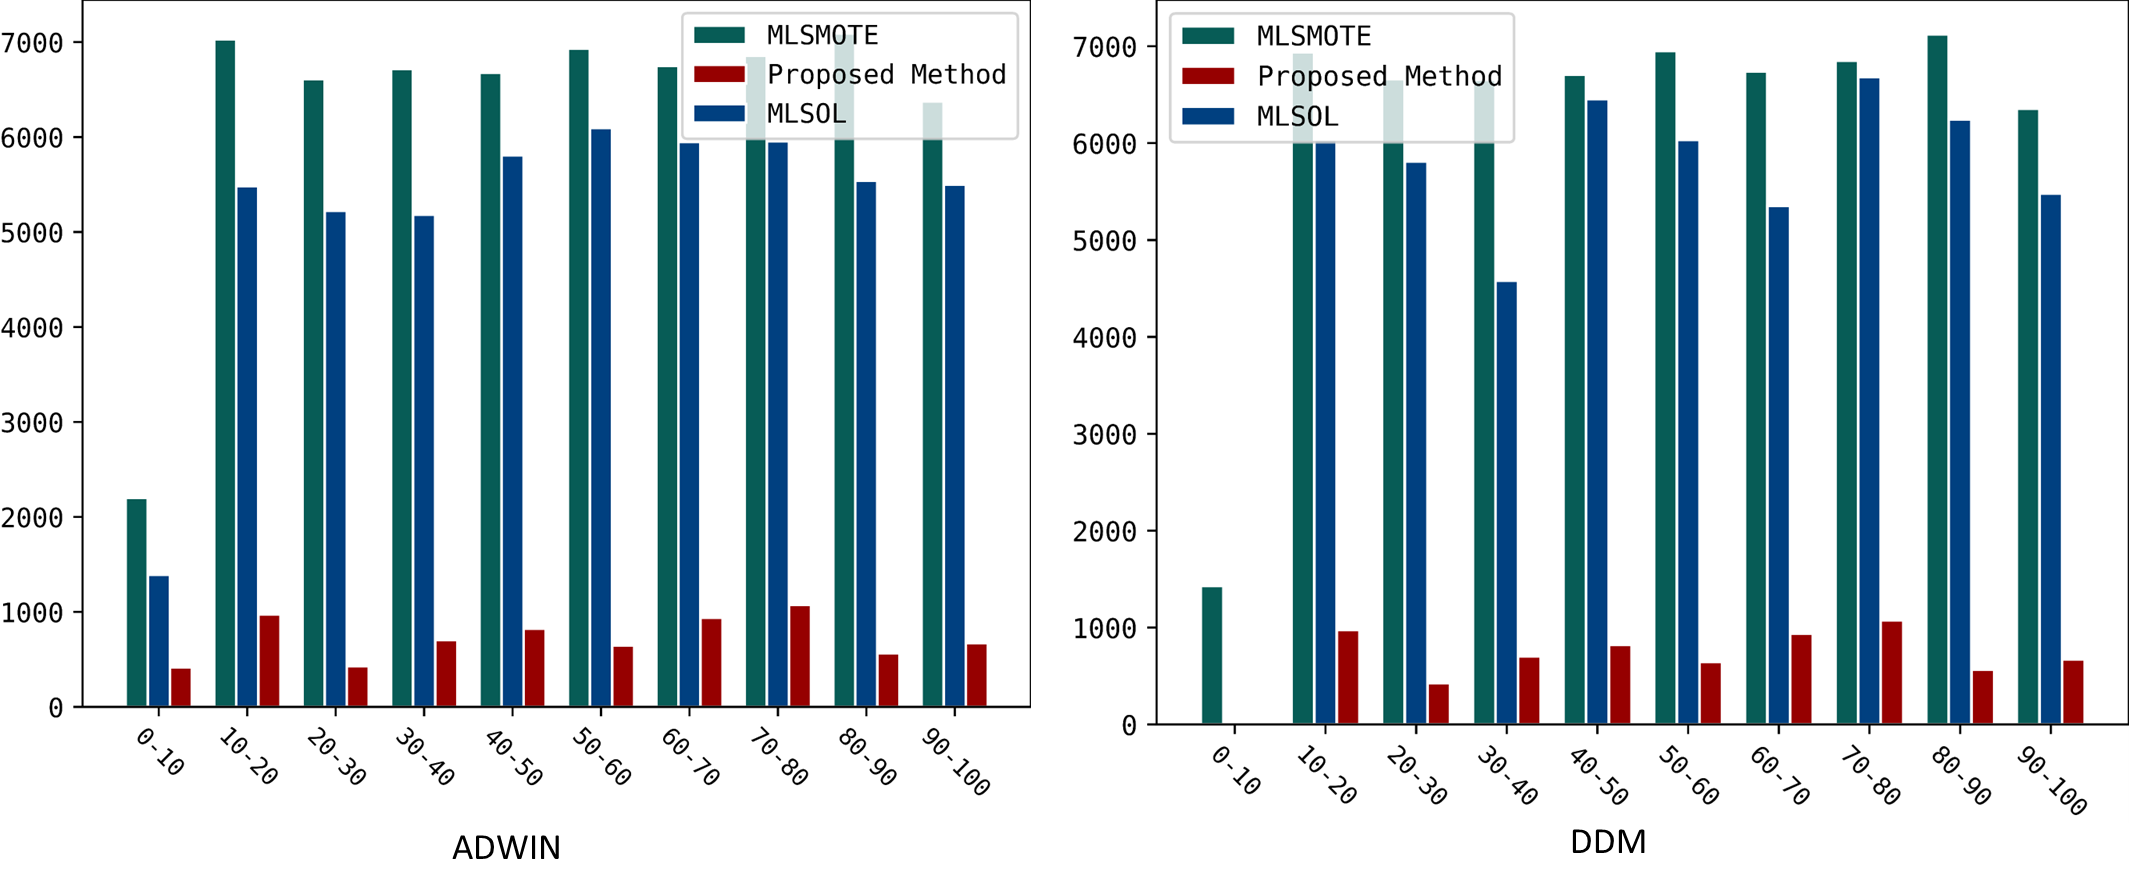
\includegraphics[width=1\linewidth]{4_Imbalanced/figures/exp_9.png}
  \caption{Overlapping generated instances of the Proposed Approach (PA), MLSMOTE, and MLSOL techniques on the synthetic stream.}
	\label{fig:4_first_proposal_result_exp_9}
\end{figure}

\subsection{Analyzing Runtime Factor Between the Proposed Approach, MLSMOTE, and MLSOL Techniques}
The results of our experiments indicate that the choice of the best algorithm for multiclass imbalanced streams depends on various factors, including dataset characteristics, the concept drift detector used, the presence of an overlapping class problem, and the algorithm's runtime demands. To investigate the runtimes of MLSMOTE, MLSOL, and our proposed approach, we conducted experiments, as shown in Table \ref{tab:4_first_proposal_result_table_2}. Our findings reveal that our proposed approach is highly efficient, regardless of whether ADWIN or DDM is used as the concept drift detector. Specifically, when ADWIN was used, the proposed approach algorithm took 8344 s to train and predict the Covertype stream for ensemble classifiers, whereas it took 8019 s when using the DDM detector. In contrast, MLSMOTE and MLSOL require more time for the same task. Notably, our proposed approach maintains efficiency, even when using the DDM concept detector. Additionally, our proposed approach demonstrates shorter processing times in the Sensor stream and synthetic data compared with other methods. Consistently, the DDM detector achieved less time across all experiments owing to its lower detection of drifts compared to the ADWIN detector. This is because there are fewer instances that trigger training for pool classifiers when using the DDM. The bold highlighting in Table \ref{tab:4_first_proposal_result_table_2} further emphasizes the efficiency of our proposed approach with both the ADWIN and DDM detectors across all dataset streams. Because our proposal generates fewer overlapped samples, leading to an overall decrease in the running time.

\begin{table}[h!]
  \centering
  \resizebox{\textwidth}{!}{
  \begin{tabular}{|l|l|c|c|c|}
  \hline
  \textbf{Stream} & \textbf{Concept Drift Detector} & \textbf{MLSMSOTE} & \textbf{MLSOL} & \textbf{PA} \\ \hline
  \multirow{2}{*}{Benchmark} & ADWIN & 9559 & 8655 & \textbf{8344} \\ \cline{2-5} 
   & DDM & 8388 & 8031 & \textbf{8019} \\ \hline
  \multirow{2}{*}{Real Application} & ADWIN & 1291 & 1310 & \textbf{1102} \\ \cline{2-5} 
   & DDM & 585 & 607 & \textbf{521} \\ \hline
  \multirow{2}{*}{Synthetic} & ADWIN & 12870 & 4866 & \textbf{4834} \\ \cline{2-5} 
   & DDM & 12397 & 4958 & \textbf{4687} \\ \hline
  \end{tabular}
  }
  \caption{Runtime of MLSMOTE, MLSOL, and the Proposed Approach (PA).}
  \label{tab:4_first_proposal_result_table_2}
  \end{table}

\subsection{Analyzing Non-parametric Tests between the Proposed Approach, MLSMOTE, and MLSOL Techniques}
We conducted a thorough series of statistical analyses encompassing 12 comparisons across three diverse datasets, three methods, and two drift detectors. These analyses were rigorously evaluated using a non-parametric test, specifically the Kruskal-Wallis test. The results of this test were striking, revealing substantial variations in the G-mean measurements across most experiments. Importantly, these differences were not due to random chance \cite{yamada2013change}. Upon closer examination of the assessments for the three methods, PA, MLSMOTE, and MLSOTE, as detailed in Table \ref{tab:4_first_proposal_result_table_3}, we found compelling evidence supporting the acceptance of the null hypothesis (H0).
This implies that the expected and observed data exhibited statistically significant disparities. H0 is rejected when significant differences are not observed and H0 is accepted if the P-value falls below the critical value. Underlining the significance of our analysis, the Kruskal-Wallis test was conducted with a 95\% confidence level, and the P-value was rounded to the first three digits after the decimal point. Nevertheless, it is important to note that a similarity in the performances of the methods emerged in the third and fourth experiments, resulting in the rejection of H0. This similarity can be attributed to the fact that the DDM detected fewer drifts in these experiments.


\begin{table}[h!]
  \centering
  \resizebox{\textwidth}{!}{
  \begin{tabular}{|c|c|c|c|c|c|}
  \hline
  \multirow{2}{*}{Dataset} & \multirow{2}{*}{Drift detector} & \multirow{2}{*}{Comparison} & \multirow{2}{*}{P-value} & \multirow{2}{*}{Critical value} & \multirow{2}{*}{H0} \\ 
                           &                                 &                             &                           &                                 &  \\
  \hline
  \multirow{4}{*}{Covertype stream} & \multirow{2}{*}{ADWIN} & PA - MLSSMOTE & 0.001 & 0.05 & Accept \\ \cline{3-6}
                                    &                        & PA - MLSOL    & 0.014 & 0.05 & Accept \\ \cline{2-6}
                                    & \multirow{2}{*}{DDM}   & PA - MLSSMOTE & 0.361 & 0.05 & Rejected \\ \cline{3-6}
                                    &                        & PA - MLSOL    & 0.401 & 0.05 & Rejected \\ 
  \hline
  \multirow{4}{*}{Sensor stream} & \multirow{2}{*}{ADWIN} & PA - MLSSMOTE & 0.001 & 0.05 & Accept \\ \cline{3-6}
                                 &                        & PA - MLSOL    & 0.001 & 0.05 & Accept \\ \cline{2-6}
                                 & \multirow{2}{*}{DDM}   & PA - MLSSMOTE & 0.001 & 0.05 & Accept \\ \cline{3-6}
                                 &                        & PA - MLSOL    & 0.001 & 0.05 & Accept \\ 
  \hline
  \multirow{4}{*}{Synthetic stream} & \multirow{2}{*}{ADWIN} & PA - MLSSMOTE & 0.001 & 0.05 & Accept \\ \cline{3-6}
                                    &                        & PA - MLSOL    & 0.001 & 0.05 & Accept \\ \cline{2-6}
                                    & \multirow{2}{*}{DDM}   & PA - MLSSMOTE & 0.001 & 0.05 & Accept \\ \cline{3-6}
                                    &                        & PA - MLSOL    & 0.001 & 0.05 & Accept \\ 
  \hline
  \end{tabular}
  }
  \caption{Kruskal-Wallis test results for MLSMOTE, MLSOL, and PA.}

  \label{tab:4_first_proposal_result_table_3}
  \end{table}

%%%%%%%%%%%%%%%%%%%%%%%%%%%%%%%%%%%%%%%%%%%%%%%
%
%   Conclusions
%
%%%%%%%%%%%%%%%%%%%%%%%%%%%%%%%%%%%%%%%%%%%%%%%

%%%%%%%%%%%%%%%%%%%%%%%% Here it is needed to re-frame the conclusions

\section{Conclusion and Future Works}
\label{sec:4_8_Conclusions}

Our study in this chapter presents a comprehensive methodology designed to facilitate incremental learning in drifted streams, with a particular focus on addressing the challenges associated with imbalanced data streams including minority and overlapping classes. The proposed methodology integrates our proposed oversampling method, concept drift detection strategies, and Dynamic Ensemble Selection (DES) to select the most suitable ensemble classifier. Extensive experimentation across various datasets, including benchmark datasets, real application streams, and synthetic data, validated the effectiveness of this contribution. The critical role of the concept drift detector in our approach lies in its capacity to promptly detect concept drifts, allowing our methodology to adapt by training new base classifiers to maintain relevance and performance in real-time scenarios. Oversampling techniques were utilized to mitigate the minority class problem, and the KNN algorithm was employed to prevent the generation of overlapped class instances. The DES technique was utilized to intelligently select the best base classifiers to ensure optimal performance. Our evaluation approach employs various performance measures, showcasing its proficiency in addressing multiclass imbalanced stream problems, particularly its exceptional performance in classifying data streams with evolving class distributions. In addition to its performance and performance, our approach has several advantages, including adaptability, efficiency, and scalability. Dynamic model updates driven by incoming data instances enable continuous adaptation to changing data distributions, thereby ensuring reliability and relevance in real-time scenarios. However, it is essential to recognize the specific limitations of the proposed approach. One limitation is the extended time required to generate nonoverlapping performance instances. Moreover, the efficacy of our contribution depends on the performance of the MLSMOTE and MLSOL techniques. Consequently, future research efforts should be directed toward enhancing our contributions. Potential avenues for improvement include the development of advanced oversampling techniques to avoid generating overlapping synthetic instances. Additionally, meta-learning methods have been explored to calculate imbalanced multiclass ratios and minority classes.


%emerging
% this file is called up by thesis.tex
% content in this file will be fed into the main document

 
% this file is called up by thesis.tex
% content in this file will be fed into the main document

%: ----------------------- introduction file header -----------------------


\begin{savequote}[50mm]
  You cannot teach a man anything; you can only help him discover it in himself.
  \qauthor{Galileo}
  % The beginning is the most important part of the work.
  % \qauthor{Plato}
  \end{savequote}
  
  
  \chapter{Dynamic Classification Ensembles for Handling Imbalanced
  Multiclass Drifted Data Streams}
  \label{chapter:5_emerging}
  
  In various real-world applications, data streams have introduced new challenges to learning algorithms. Data streams are continuous with high volumes of data arriving rapidly and dynamically. This data deluge poses unprecedented challenges for learning algorithms because they must adapt to the dynamic nature of the data environment \cite{yang2021concept}\cite{dong2019multistream}\cite{shan2018online}. Among the various research areas in machine learning, incremental learning under data Streams with Emerging New Classes (SENC) has garnered considerable attention because of its practical relevance and unique challenges \cite{da2014learning}\cite{mu2017streaming}\cite{zhu2020semi}. SENC refers to a scenario in which new classes that were not present during the initial training of a learning model emerged in the data stream. This poses a significant challenge for traditional learning approaches that are typically designed to handle fixed or predefined class distributions. The ability to effectively recognize and adapt to these novel classes in real-time is crucial for maintaining accurate and up-to-date models. Furthermore, the inherent limitations of data streams, such as limited memory and storage constraints, impose additional complexities in the learning process. Learning algorithms must operate efficiently within these resource constraints to ensure real-time processing and to avoid overwhelming computational overhead.
  To address the challenges presented by data streams containing emerging new classes, dynamic ensemble selection (DES) \cite{cruz2017meta}\cite{jackowski2014improved}\cite{kuncheva2000clustering}. Dynamic ensemble selection involves utilizing multiple classifiers in machine learning to make collective predictions or classifications of data. Dynamic ensemble selection is distinguished by its ability to dynamically adapt the ensemble based on the characteristics of the data. Instead of relying on a fixed ensemble of classifiers, dynamic ensemble selection continuously assesses the performance of individual classifiers and selects the subset that demonstrates the highest competence for the current data. This adaptability enables the ensemble to enhance its performance over time by incorporating the most suitable classifiers for prevailing data conditions. Furthermore, if a classifier becomes ineffective owing to concept drift or the emergence of new classes, it can be excluded from the ensemble to prevent it from negatively affecting the overall performance.
   Adaptive Windowing (ADWIN) is another widely employed method to address concept drift. Concept drift refers to the phenomenon in which the statistical properties of data change over time, leading to a decline in the learning algorithm performance \cite{gama2004learning}\cite{adams2023explainable}\cite{madkour2023historical}. ADWIN continuously monitors incoming data and detects changes or drifts in data distribution. It achieves this by maintaining sliding windows of variable sizes and monitoring statistical measures such as the mean or variance within these windows. Upon detecting a significant change or drift, the ADWIN triggers an update in the ensemble or classifier configuration. This update may involve retraining the classifiers with new data or incorporating new classifiers that are better suited to the updated data distribution. By adapting the ensemble to changing data conditions, ADWIN ensures that the classifier system remains accurate and up-to-date even in the presence of concept drift or the emergence of new classes. The primary objective of utilizing these approaches, such as dynamic ensemble selection and ADWIN, is to establish a flexible and effective classification system that is capable of handling data streams containing emerging new classes. By dynamically adjusting the ensemble based on the data characteristics and detecting and adapting to concept drift, these approaches enable the system to maintain accurate predictions over time. Adaptability and responsiveness are crucial for addressing the unique challenges posed by the dynamic nature of data streams and the emergence of new classes within them.  
  This research proposes efficient algorithms for classifying data streams in real-time scenarios, focusing on addressing the challenges posed by emerging new classes in data distributions. 
  The subsequent sections of this paper adhere to a well-structured organization. Section 2 presents a comprehensive review of the relevant literature encompassing concept drift, dynamic classifier ensembles, and emergency class detection methods. Section 3 introduces the proposed framework, providing intricate explanations of its constituents, including dynamic classifier ensembles, concept drift handling, and emergency class identification, and the adaptive proposed method of the emerging pool size. Section 4 outlines the experimental setup and presents the results, providing details regarding the employed datasets, evaluation metrics, and procedures. Finally, in Section 5, we offer concluding remarks, summarizing the key findings, discussing their implications, and proposing potential avenues for future research.
  
  
  The remainder of this chapter is organized as follows: In Section \ref{sec:5_2_motivation}, we present the motivations and the contributions. The proposed framework and combination via SI algorithms are discussed in detail in Section \ref{sec:5_4_proposed}. The  experimental results and the discussion are presented in Sections \ref{sec:5_5_Expsetup} and \ref{sec:5_7_Discussion}, respectively. Finally, the conclusions of this study and future research are discussed in Section \ref{sec:5_8_Conclusions}. 
  
  
  \section{Motivations and Contributions} \label{sec:5_2_motivation}
  We aim to develop novel algorithms that can effectively handle the emergence of new classes issue in nonstationary data streams, achieve high classification accuracy, and minimize computational complexity. The key contributions of this study are outlined as follows:
   
  \begin{enumerate}[nosep]
    \item Our first contribution involves utilizing the ADWIN, DES, and K-means techniques in combination with the ensemble stratified bagging technique to detect and adapt to emerging new classes. This approach allows us to dynamically update the classification model to accommodate an evolving data environment.
   \item The second contribution is the introduction of an adaptive method to adapt the emerging pool size depend on the stream distribution.
    \end{enumerate} 
   
     
  
  
 
   



\section{Proposed Methodology}\label{sec:5_first_proposed_approach}

In this section, we present the primary phases of our study, which consist of three distinct steps designed to address the challenges of handling emerging new classes in drifted streams. Our proposed approach aims to develop a robust framework capable of tackling these complex challenges through a comprehensive, three-step methodology.
\begin{itemize}
	\item \textbf{Emerging New Classes:} Our study addresses the widespread issue of emerging new classes in drifted streams using well-known techniques, including concept drift detection and K-means clustering.
	\item \textbf{Drifted Streams: } To handle changes in the data distribution, our approach integrates a concept drift detector that dynamically identifies shifts, allowing the model to promptly adapt its classifiers to maintain effectiveness.
	\item \textbf{Classifier Performance:} The final phase identifies unknown classes in drifted streams, creating new classifiers for emerging classes to improve the model's ability to classify new instances accurately.
\end{itemize}

\subsection{THE PROPOSED APPROACH Flow}

Our proposed approach is designed with three distinct phases that work together to improve its performance in managing multiclass imbalanced and drifting data streams. 
\begin{itemize}
	\item \textbf{DES Phase (dynamic ensemble selection phase):} The first phase, known as the dynamic ensemble selection (DES) phase, is responsible for selecting the most appropriate classifier for the incoming data. This ensures that the selected classifier is well-suited for the current data chunk.
	\item \textbf{Drift detector phase:} The second phase of our approach is the drift detector phase, which operates in real-time to continuously monitor the data stream. Its primary function is to identify any signs of concept drift, which indicates shifts in the underlying data distribution over time.
	\item \textbf{Emerging New Class Identifier Phase:} The final phase of our approach is the synthetic data generator phase, which is dedicated to generating synthetic data for the minority classes. This step is crucial for addressing class imbalance by producing additional samples for underrepresented classes, thereby significantly enhancing the model's ability to accurately classify instances from minority classes.
\end{itemize}

As depicted in Fig. \ref{fig:5_first_proposal_step_1}, the DES phase retrieves the current data chunk and applies the DES technique to select the best classifiers for the chunk (black box of Fig.  \ref{fig:5_first_proposal_step_1}). These classifiers are used in the second phase to predict class labels, while drift detectors like ADWIN or DDM monitor for concept drift. If a drift is detected (highlighted by the red rectangle), the chunk is forwarded to the third phase, where new classes are identified (see Fig.  \ref{fig:5_first_proposal_step_2}). The overall approach is implemented in Algorithm  \ref{alg:5_1}, which takes a data stream and a DES Pool threshold as inputs. Key components include training the initial ensemble (Lines 4-6), using DES to select the best classifier for the current chunk (Line 8), detecting drifted chunks (Line 10), creating new classifiers for emerging classes (Line 12), and removing the worst classifier if the DES Pool threshold is exceeded (Lines 14-16).


\subsection{Emerging New Classes Phase Details}

In this section we present the Emerging new classes phase details. As shown in Fig.2, The emerging phase contains two primary steps: 
\begin{itemize}
	\item 	\textbf{Emerging new classes identifier:} The emerging class detection step plays a crucial role in the proposed approach (the black rectangle of Fiq.2) by utilize the K-means technique to clustering the drifted chunk into a set of clusters. And identifying new emerging classes by evaluating the distances between instances and their nearest class centroid. This process involves comparing the distance between an instance and the nearest class centroid with the maximum distance between class centroids ($d_c$), as described in Eq. \ref{eq:5_first_proposal_1} and Eq. \ref{eq:5_first_proposal_2}, where ED represents the Euclidean Distance method and ci, cj denotes the centroids of the current classes. If the calculated distance ($d_x$) exceeds this threshold ($d_c$), this indicates the presence of a new emerging class, denoted by EC in Eq. \ref{eq:5_first_proposal_3}; otherwise, it is $P_\text{DES}$ (prediction class of the new instance).
	\item \textbf{Adaptive the Emerging classes pool size:} This critical step adapts the pool size based on the emergence rate of new classes and drift distribution, using statistical measures like standard deviation, first derivative, and average historical drift updates.
	The Emerging New Classes phase is implemented in Algorithm  \ref{alg:5_2}, which utilizes drifted instances and current changes as inputs. Key steps include applying K-means (Line 1), calculating cosine similarity between centroids (Line 2), determining the maximum centroid distance (Line 3), setting the adaptive pool threshold (Lines 4-7), using KNN to find the nearest neighbor (Line 9), storing instances in the emerging pool if the distance exceeds the threshold (Lines 11-12), and creating a new classifier if the pool size surpasses the adaptive limit (Lines 14-17). A simulated scenario is illustrated in Figures 3 and 4. In Fig. \ref{fig:5_scenario1}(a), the drifted chunk is divided into three clusters using the K-means algorithm. Fig. \ref{fig:5_scenario1}(b) shows the calculation of the maximum distance between cluster centroids, which serves as a threshold for identifying new classes. The procedure for classifying instances is as follows: when a drifted instance is detected, it is considered a new class if the distance between the instance and its nearest centroid exceeds the maximum inter-centroid distance (Fig. \ref{fig:5_scenario2} a). If the distance is within the threshold, the instance is classified as a known class (Fig. \ref{fig:5_scenario2} b).
\end{itemize}

\begin{figure}[!ht]
	\centering
	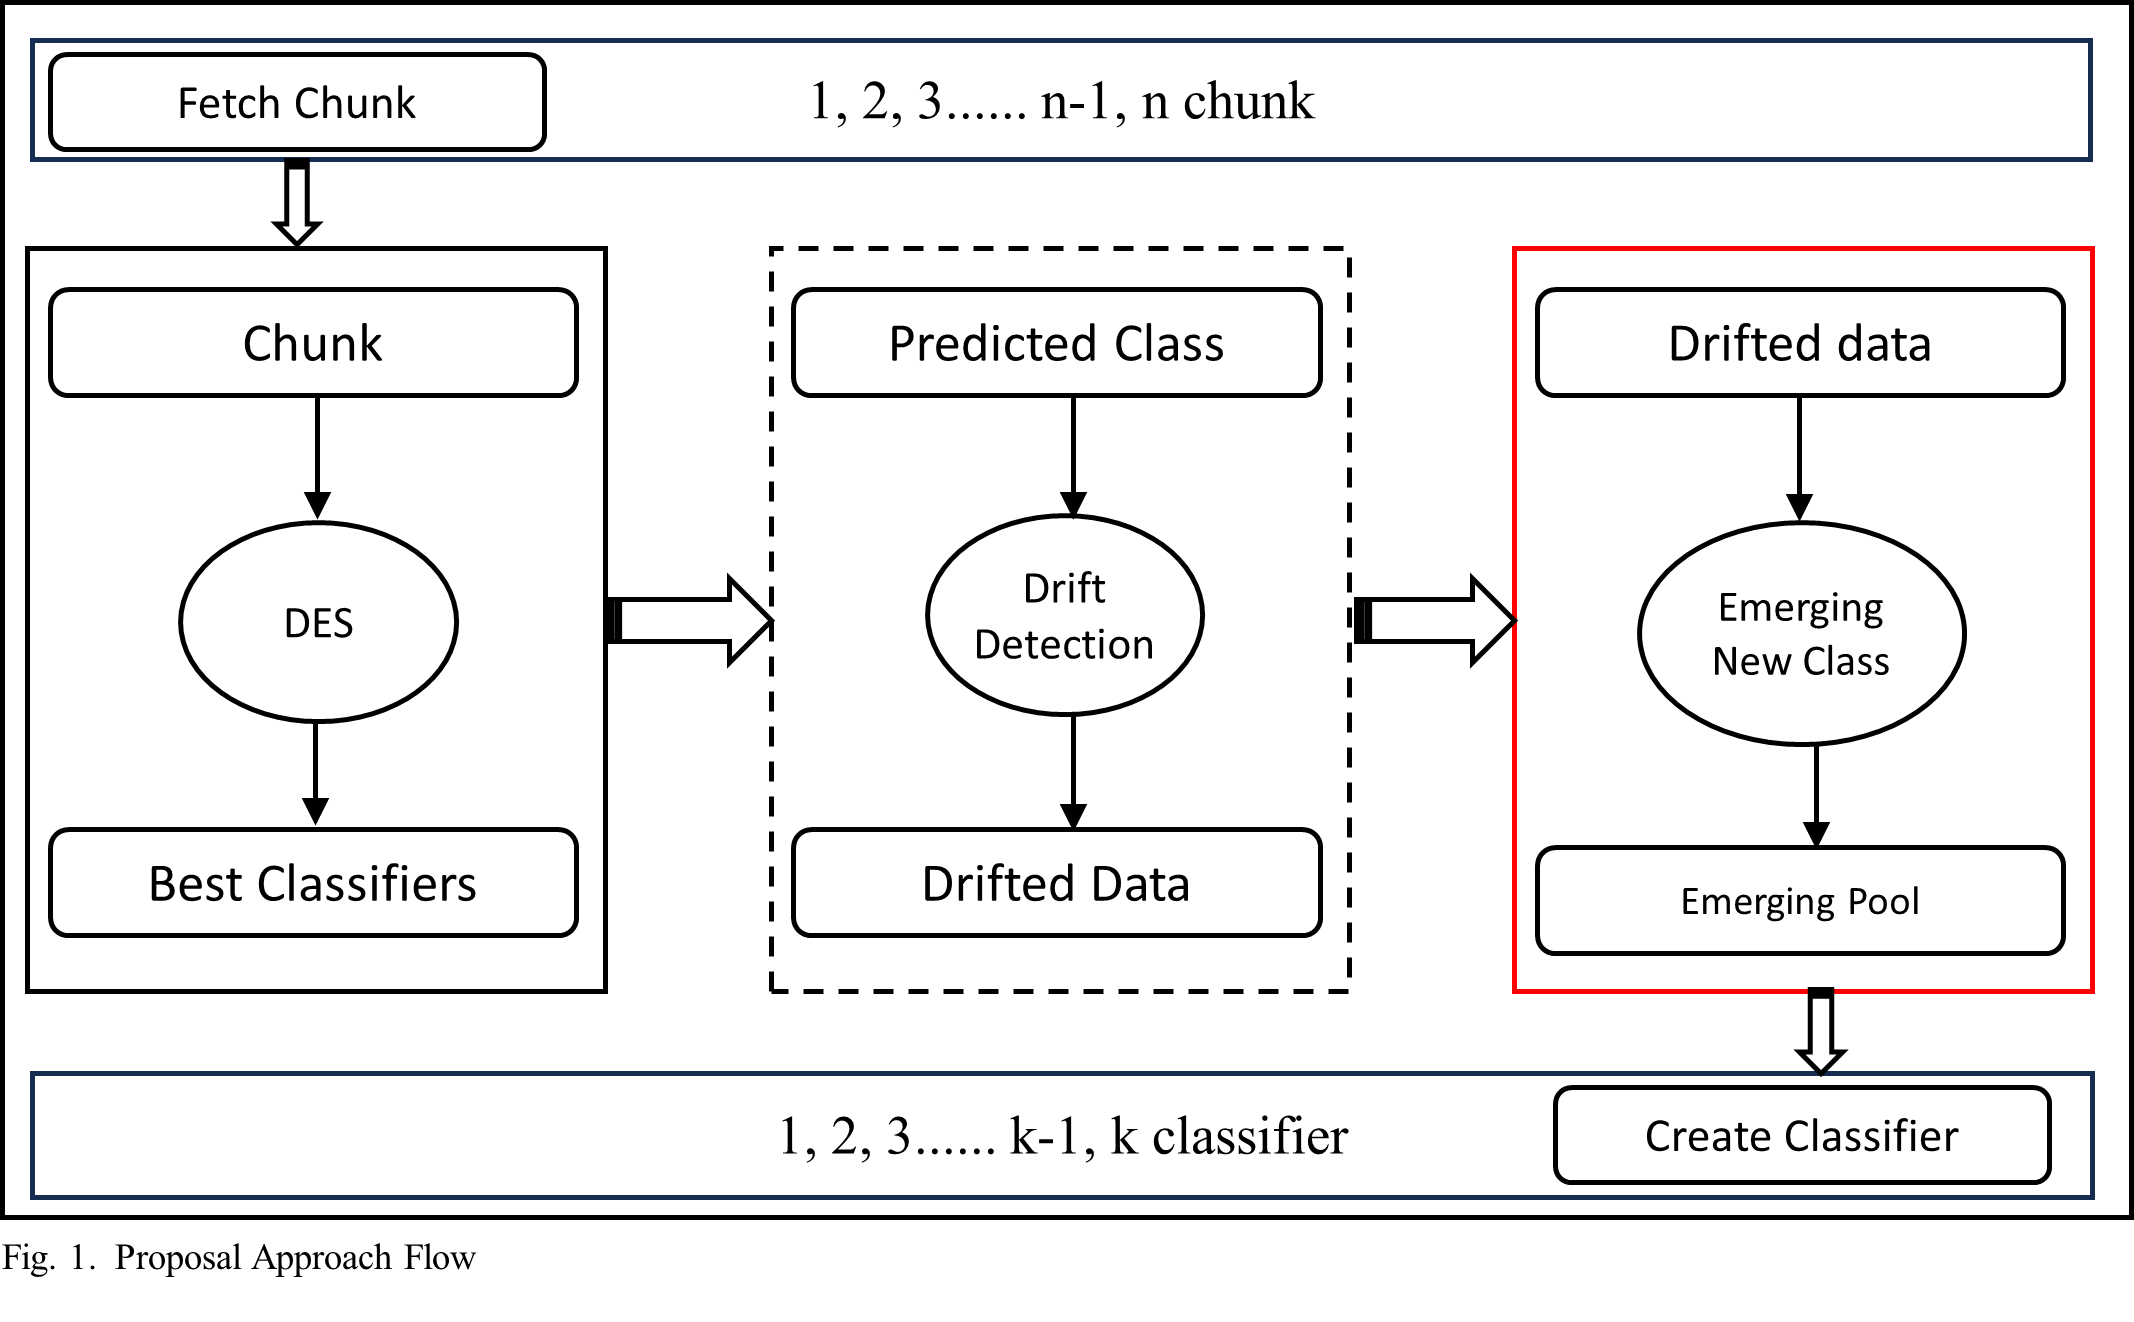
\includegraphics[width=1\linewidth]{5_Emerging/figures/algorithm1.png}
	\caption{Proposed Approch Flow}
	\label{fig:5_first_proposal_step_1}
\end{figure}
\begin{figure}[!ht]
	\centering
	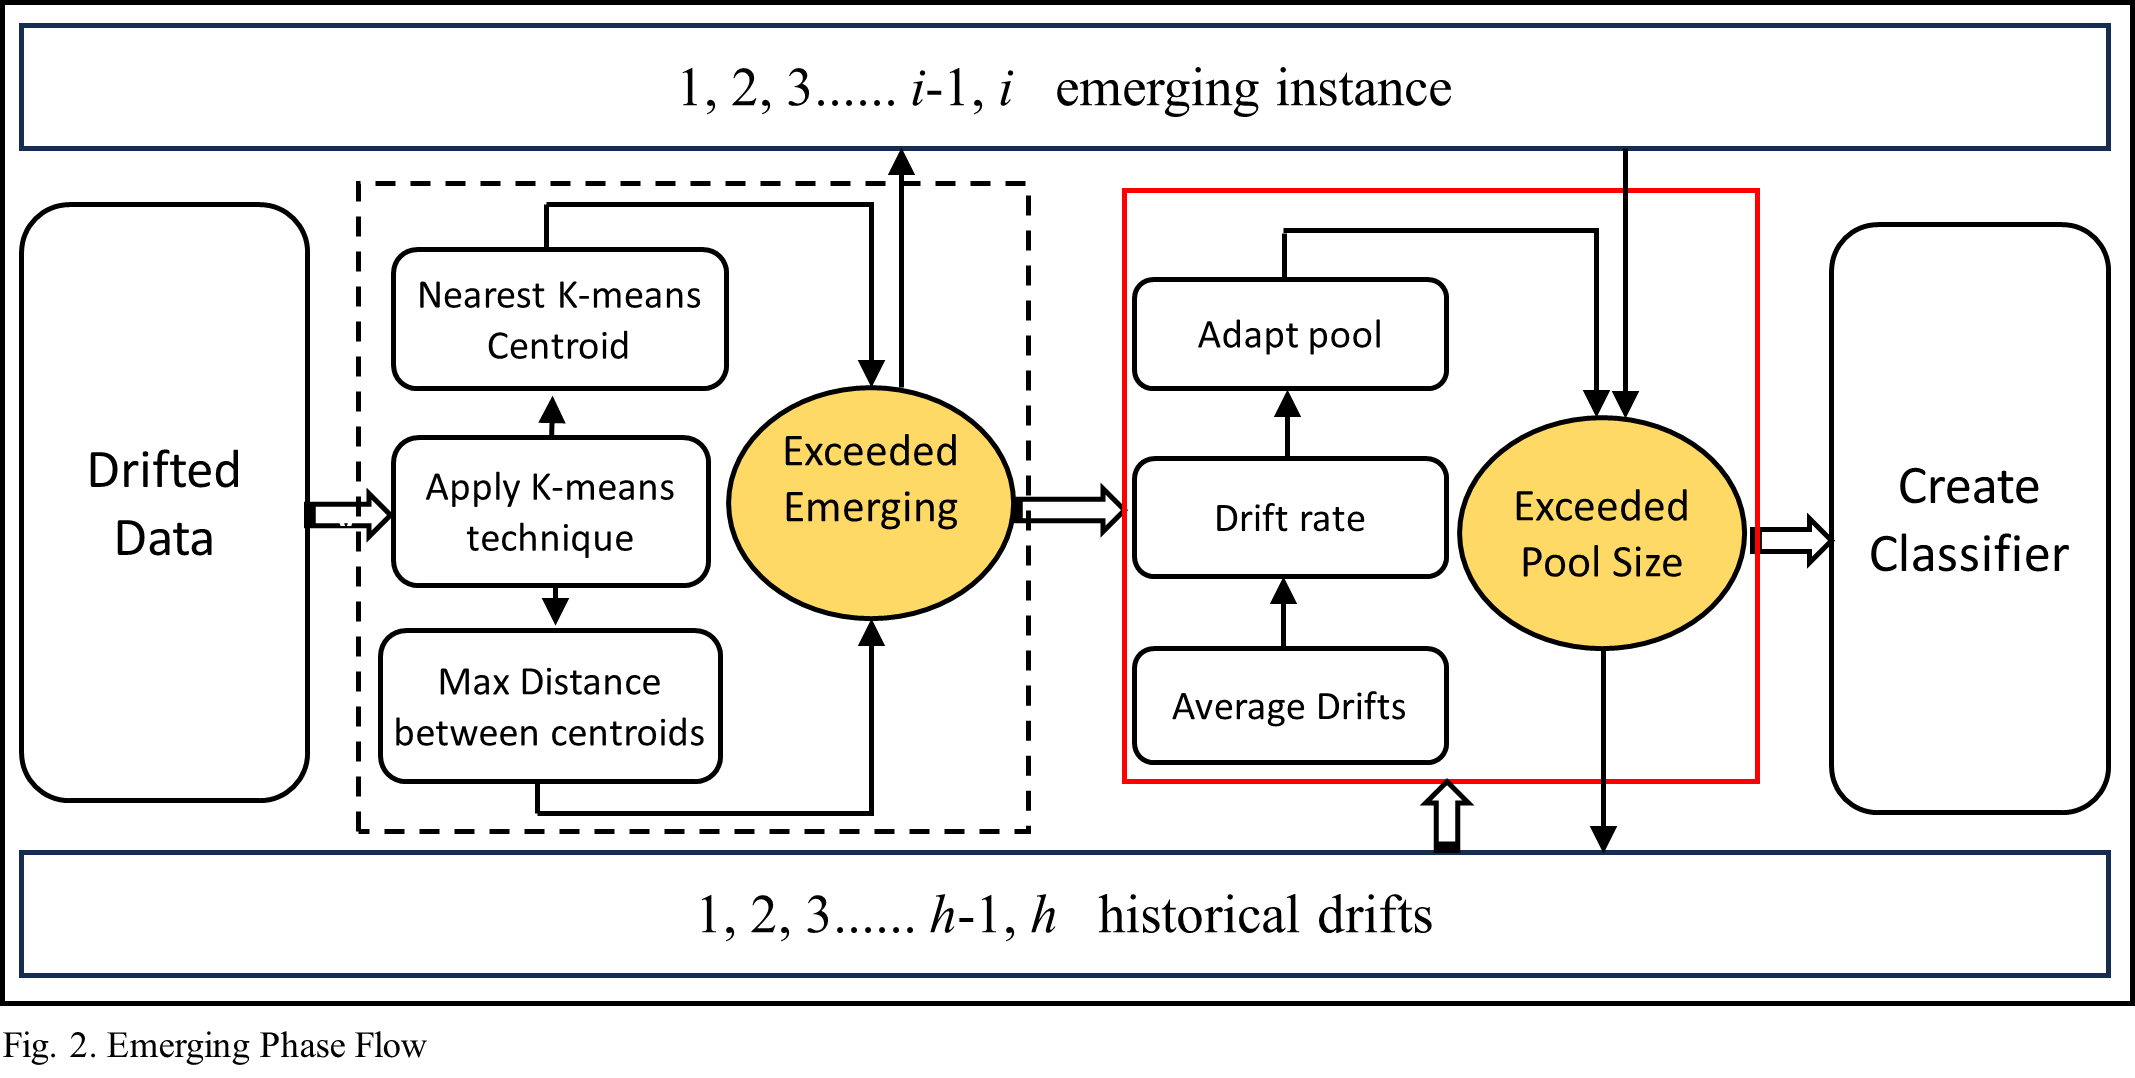
\includegraphics[width=1\linewidth]{5_Emerging/figures/algorithm2.png}
	\caption{Emerging Phase Flow}
	\label{fig:5_first_proposal_step_2}
\end{figure}
\begin{figure}[!ht]
	\begin{center}
	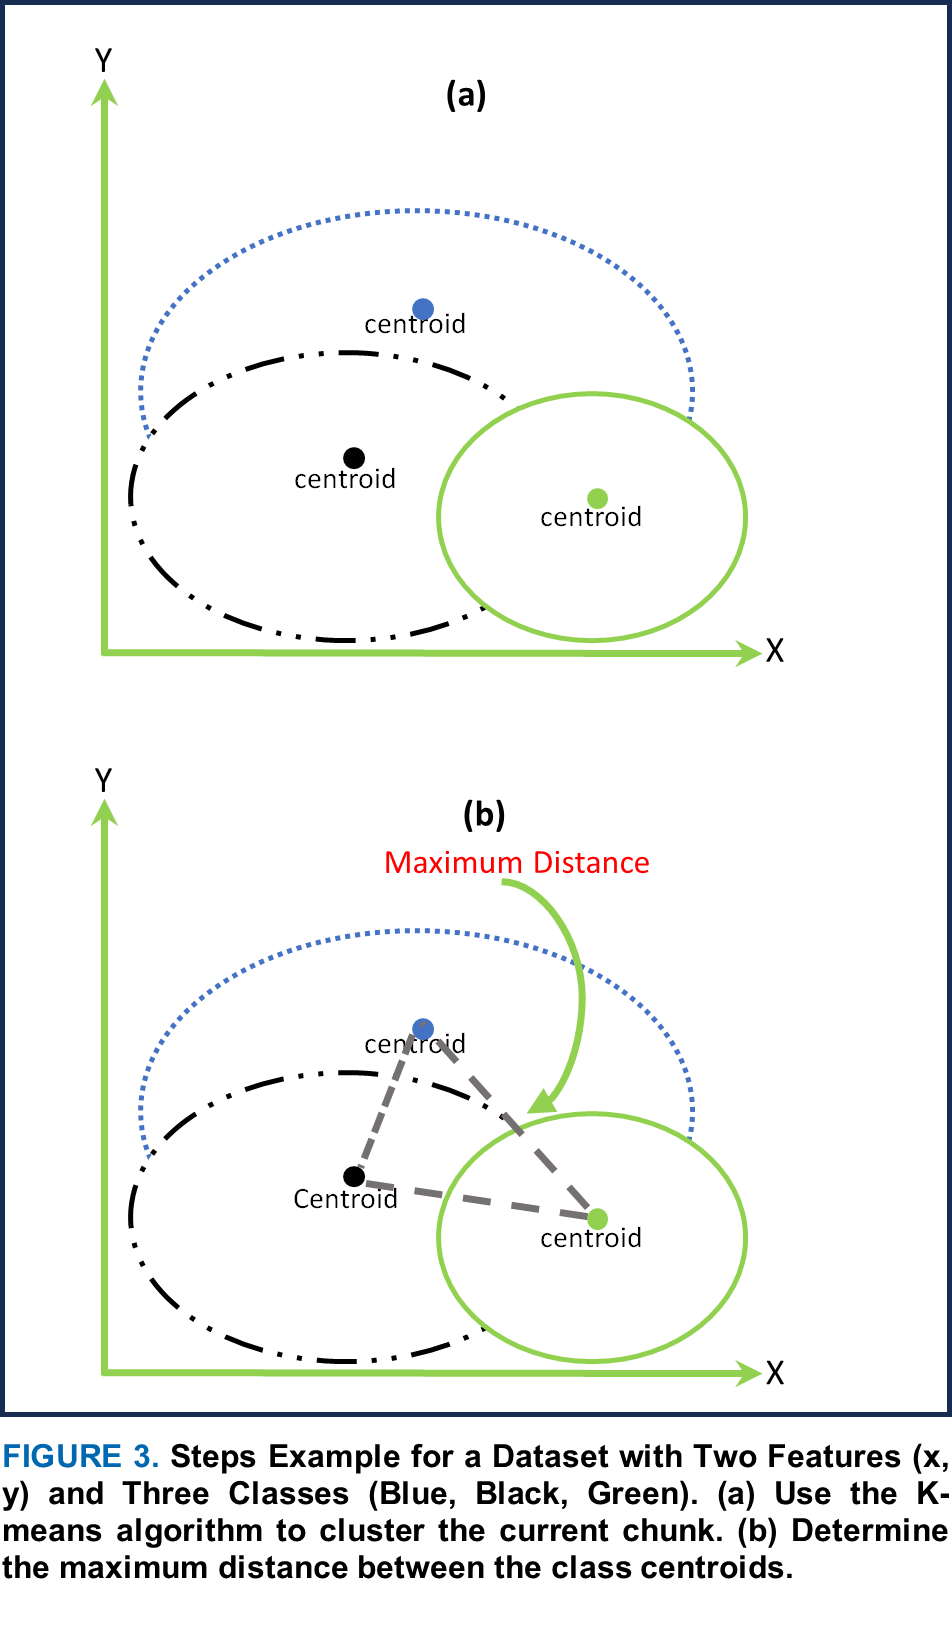
\includegraphics[width=0.48\linewidth]{5_Emerging/figures/scenario1.png}
	\caption{Proposed Approch Flow}
	\label{fig:5_scenario1}
	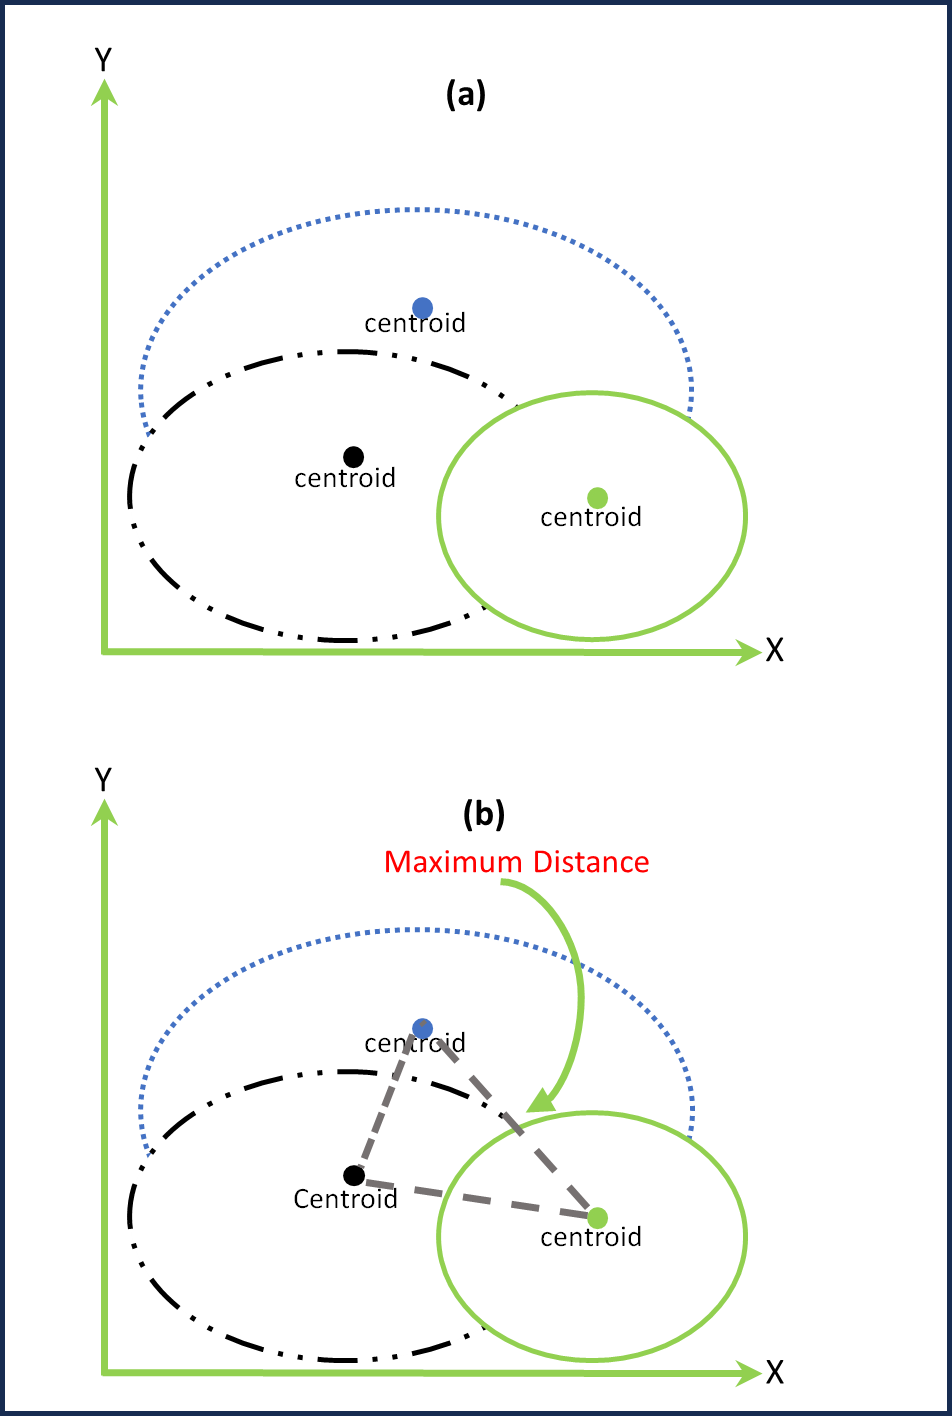
\includegraphics[width=0.48\linewidth]{5_Emerging/figures/senario2.png}
	\caption{Emerging Phase Flow}
	\label{fig:5_scenario2}
\end{center}

\end{figure}

\begin{equation}
	\label{eq:5_first_proposal_1}
    d_c = \arg\max_d \sum_{i=1}^{i} \sum_{j=i+1}^{i} d = ED(c_i, c_j)
\end{equation}

\begin{equation}
	\label{eq:5_first_proposal_2}
	d_x = \arg\min_i \sum_{i=1}^{i} ED(x, c_i)
\end{equation}

\begin{equation}
	\label{eq:5_first_proposal_3}
    \begin{cases}
		EC & \text{if } d_x > d_c \\
		P_{DES} & \text{otherwise}
	\end{cases}
\end{equation}

\begin{algorithm}[H]
	\caption{Proposed Framework Algorithm for Imbalanced Multi-Class Drifted Data Streams}
	\label{alg:5_1}
	\KwIn{data stream, maximum classifiers pool size $\kappa$}
	% \Parameter{current chunk $a$, synthetic data $b$, classifiers pool $\Psi$, drifted pool $\psi$, classes frequency $\Omega$, best frequency $\omega$, minority classes $\mu$}
	\KwOut{Prediction $P$}
	\BlankLine
	$\psi, \Psi, \Omega, \mu \gets \emptyset$\;
	$\omega \gets 0$\;
	\For{stream have chunk}{
		\eIf{$a$ is the First chunk}{
			$k \gets$ \texttt{trainingNewClassifier}($a$)\;
			$P \gets$ \texttt{getPrediction}($a, k$)\;
		}{
			$k \gets$ \texttt{DES}($a, \Psi$)\;
			$P \gets$ \texttt{getPrediction}($a, k$)\;
			$\psi \gets$ \texttt{conceptDriftDetector}($P$)\;
			\If{$\psi > 0$}{
				$\Omega \gets$ get classes frequency according to Eq.1\;
				$\omega \gets$ best frequency according to Eq.2\;
				$\mu \gets$ get minority classes according to Eq.3\;
				$b \gets$ utilize $a$ and $\mu$ to get the synthetic data according to Algorithm 2\;
				trainingData $\gets a + b$\;
				$k \gets$ \texttt{trainingNewClassifier}(trainingData)\;
				$\Psi \gets \Psi + k$\;
				\If{$\Psi > \kappa$}{
					\texttt{removeWorstClassifier}($\Omega$)\;
				}
			}
			$P \gets$ \texttt{getPrediction}($a, k$)\;
		}
	}
	\Return{$P$}
	\end{algorithm}
	
	\vspace{1cm}
	
	\begin{algorithm}[H]
		\caption{Synthetic data generator}
		\label{alg:5_2}
		\KwIn{Minority classes $\mu$, current chunk $a$, sample size $\eta$, historical chunks $h$}
		\KwOut{Generated data $b$}
		$b \gets \emptyset$\;
		$f \gets \text{MLSMSOTE}$\;
		$knn \gets \text{kNearestNeighbor}(a)$\;
		$chunk \gets \text{similarChunk}(a, h)$\;
		$f \gets \text{similarChunkOverSamplingMethod}(chunk)$\;
		\If{$f = \text{MLSMSOTE}$}{
			$f \gets \text{MLSOL}$\;
		}
		\Else{
			$f \gets \text{MLSMSOTE}$\;
		}
		\While{$|b| < \eta$}{
			$p \gets \text{generateSyntheticPoint}(\mu, f)$\;
			$similarPointsClass \gets \text{KNN.getKneighbor}(b)$\;
			\If{$similarPointsClass = \mu$}{
				$b \gets b \cup \{p\}$\;
			}
		}
		\Return $b$\;
		\end{algorithm}


%transfer
\chapter{Dynamic Classification Ensembles for Handling Imbalanced
Multiclass Drifted Data Streams}
\label{chapter:6_transfer_learning}

Transfer learning plays a pivotal role in addressing the intricate challenges posed by dynamic data streams and inherent concept drifts. Transfer learning aims to enhance a model's learning performance within a target domain by leveraging the knowledge gleaned from the source domains \cite{pan2009survey}\cite{wang2019characterizing}. This research domain focuses extensively on addressing target tasks that grapple with limited or unlabeled data, with a dual emphasis on amplifying positive knowledge transfer and alleviating negative knowledge transfer \cite{wang2019characterizing}. To facilitate the transfer of valuable knowledge, researchers have developed diverse techniques, including methodologies aimed at reducing the domain gap, such as instance re-weighting \cite{zadrozny2004learning}\cite{cortes2008sample}\cite{pan2010domain} and feature matching \cite{sun2016return}\cite{pan2010domain}. Conversely, strategies for mitigating negative knowledge transfer often involve down weighting irrelevant data sources \cite{wang2019characterizing}.
Although a substantial body of transfer learning research has focused on static environments, where data in each domain are assumed to conform to the same distribution, real-world scenarios, including financial data analysis, energy demand prediction, and climate data analysis, often involve dynamic environments. Within these dynamic contexts, the concept drift problem \cite{li2015learning}\cite{cao2019learning} emerges as data distributions evolve over time. Dynamic environment transfer learning requires continuous adaptation to concept drift and adaptive utilization of valuable knowledge from source domains within each distinct environment. These new challenges in transfer learning, particularly within dynamic environments, represent a profound departure from traditional transfer learning paradigms that do not inherently address concept drift and the dynamic nature of evolving data.
To overcome these challenges, Dynamic Ensemble Selection (DES) \cite{cruz2017meta}\cite{jackowski2014improved}\cite{kuncheva2000clustering}, ADWIN, and Streaming Ensemble Algorithm (SEA) have become prominent in the scientific literature \cite{gama2004learning}\cite{adams2023explainable}\cite{madkour2023historical} Dynamic ensemble selection employs multiple classifiers within the realm of machine learning to make collective predictions or classifications, and leverage data characteristics. Its key feature is its dynamic adaptability, as it continuously evaluates the performance of individual classifiers and selects a subset that demonstrates the highest competence within the prevailing data conditions. This adaptability empowers the ensemble to progressively enhance its performance by incorporating best-fitting classifiers for the existing data context. Moreover, ineffective classifiers can be excluded from the ensemble in scenarios marked by concept drift, thereby protecting the overall performance from detrimental effects.
Adaptive Windowing (ADWIN) is another widely used method designed to address the challenges of concept drift \cite{madkour2023historical}. Concept drift refers to the phenomenon in which the statistical properties of data change over time, leading to a decline in the learning algorithm performance. ADWIN monitors incoming data by maintaining sliding windows of variable sizes and evaluating statistical attributes, such as the mean or variance within these windows. Upon detecting substantial shifts or drifts, the ADWIN initiates adjustments to the ensemble or classifier configuration. These adjustments may involve retraining classifiers with fresh data, or incorporating new classifiers that are better suited to the updated data distribution. Additionally, the Streaming Ensemble Algorithm (SEA) is an integral component for addressing these dynamic challenges \cite{gama2004learning}\cite{adams2023explainable}\cite{madkour2023historical}. SEA is specifically designed to manage data streams and inherent concept drifts. This is achieved by adapting the ensemble of classifiers in real time as new data arrives. SEA's adaptability of SEA ensures that the ensemble remains robust and accurate even in the face of shifting data conditions and the emergence of new classes.
This study proposes efficient algorithms for classifying data streams in real-time scenarios, focusing on addressing the challenges posed by heterogeneous transfer learning in data distributions. The goal is to develop a novel algorithm (Heterogeneous Transfer Learning) that can effectively handle non-stationary data streams, achieve high classification accuracy, and minimize computational complexity. 
The subsequent sections of this paper adhere to a well-structured organization. Section 2 comprehensively reviews the relevant literature on concept drift and transfer learning. Section 3 introduces the proposed approach, providing intricate explanations of its constituents, including dynamic classifier ensembles, concept drift handling, and heterogeneous multisource transformation. Section 4 outlines the experimental setup and presents the results, providing details regarding the employed datasets, evaluation metrics, and procedures. Finally, in Section 5, we offer concluding remarks, summarizing the key findings, discussing their implications, and proposing potential avenues for future research.
\section{Motivations and Contributions} \label{sec:4_2_motivation}
This paper presents a novel contribution to real-time streaming scenarios by addressing the challenges of heterogeneous multisource streams, with key contributions that can be summarized as follows:
\begin{enumerate}[nosep]
  \item The primary innovation involves incorporating a concept drift detection method in conjunction with an ensemble classifier, enabling real-time adaptation and refinement of the proposed approach in response to transfer learning in non-stationary environments. This methodology ensures continuous evolution of the classification model in accordance with the changing data landscape.
  \item The second significant advancement is the introduction of a precise weighting method to assess the significance of each local classifier within the ultimate classifier.
 \item The third significant contribution is the development of an innovative approach that employs the eigenvector technique to facilitate the transfer of knowledge from heterogeneous source domains to the target domain.
  \end{enumerate} 
 
   


\section{Third Proposed Methodology}\label{sec:6_third_proposed_approach}

In this section, we introduce the Heterogeneous Transfer Learning (HTL) algorithm tailored for non-stationary environments. HTL adeptly assimilates knowledge from both heterogeneous and homogeneous sources, operating within the framework of data streams subject to concept drift. Leveraging an online learning inductive parameter transfer strategy, HTL achieves seamless knowledge transfer. We delineate the core components and workflow of the HTL algorithm. To address the challenges intrinsic to our approach, we focus on three key aspects:
\begin{itemize}
	\item \textbf{Heterogeneous sources:} Traditional transfer learning methods often assume homogeneity in the data distribution across source and target domains. However, in real-world scenarios, data sources may vary significantly in terms of feature space. HTL addresses this challenge by allowing knowledge transfer from sources with different dimensionalities. This means that the algorithm can effectively learn from diverse dimentionality sources, enabling a more comprehensive knowledge transfer process.
	\item \textbf{Drifted streams:} In dynamic environments, data distributions may change over time, leading to concept drift. This phenomenon poses a significant challenge for machine learning algorithms, as models trained on historical data may become obsolete as the underlying data distribution shifts. HTL incorporates a concept drift detector that continuously monitors the incoming data stream. Upon detecting a shift in the data distribution, the algorithm adapts its classifiers accordingly to ensure continued effectiveness in handling drifting streams. This dynamic adjustment mechanism allows HTL to maintain high performance even in the presence of concept drift.
	\item \textbf{Classifier performance:} Classifier performance is crucial for the overall effectiveness of the transfer learning process. HTL employs Dynamic Ensemble Selection (DES) to enhance classifier performance. DES creates a diverse ensemble of classifiers, each trained on different subsets of the data. When presented with a new data point, DES dynamically selects the most suitable classifiers from the ensemble based on its performance on similar chunk. This adaptive selection process ensures that the most appropriate classifier is chosen for each data point, leading to improved classification accuracy and robustness. By leveraging DES, HTL maximizes the utility of available classifiers, resulting in superior performance in non-stationary environments with heterogeneous data sources.
\end{itemize}

\subsection{HTL Overall Details}

The aim of this section is to harness knowledge from diverse dimensional multisource domain streams. Following a similar framework to CDTL \cite{yang2021concept}, this approach employs a class-wise and domain-weighted strategy. However, HTL enhances the weight function of CDTL in a class-wise manner, as demonstrated in Equation 1. This equation factors in both correct and incorrect predictions for each classifier class, with K representing the number of classifiers in the current chunk, C denoting the number of classes in the current chunk, and i indicating the current chunk. The components of HTL operate synergistically, as depicted in Fig. \ref{fig:6_alg1}, encompassing three phases:
\begin{itemize}
	\item \textbf{Dynamic ensemble selection phase (DES Phase):}: The primary objective DES phase is to identify the optimal classifier for incoming data. This is crucial for ensuring that the selected classifier effectively aligns with the unique characteristics of the current data segment.
	\item \textbf{Drift detector phase:} After the DES phase, our method advances to the drift detector phase, where it operates in real-time to continually monitor the data stream. This phase employs ADWIN and DDM techniques, which play a pivotal role in swiftly identifying any signs of concept drift. These techniques are designed to detect changes in the underlying data distribution over time, thus enabling the algorithm to adapt to evolving data patterns.
	\item \textbf{Feature scaling} The concluding phase of our approach is featuring scaling, operating in real-time to harmonize the diverse dimensionalities of the multisource streams with the target dimensionality. Leveraging the eigen vector technique, this phase facilitates the transformation of data into a unified dimensionality, essential for creating new classifiers tailored to the target and domain streams. By ensuring compatibility with the learning framework, this process enhances the algorithm's effectiveness in handling diverse dimensionality streams.
\end{itemize}
\subsection{Classifier Creation Details }

Fig. \ref{fig:6_alg2} provides a comprehensive overview of the classifier creation phase, a crucial component responsible for generating new classifiers based on the current chunk of the target domain, previous classifiers, and source domain classifiers. This phase offers several advantages and perform three tasks. \begin{itemize}
	\item \textbf{Source projection:} This step involves projecting the source domain classifiers onto the current chunk of the target domain. The projection likely employs the source weight function, as described in CDTL \cite{yang2021concept}, to assign a weight to each classifier based on its relevance to the current chunk of data. This weighting mechanism ensures that classifiers from the source domains contribute appropriately to the creation of the new classifier for the target domain.
	\item \textbf{Class-wise weights:} This block computes class-specific weights for each classifier using Equations \ref{eq:6_eq_1} and \ref{eq:6_eq_2} . The process involves analyzing the current chunk of the target stream (denoted as \emph{D}) and considering both correct and incorrect predictions made by each classifier where $prediction_i$ refers to the predicted class of the current instance and $c$ to the income class. These weights are crucial for determining the significance of individual classifiers across different classes. The equations facilitate the calculation of weights that reflect the classifiers' performance on specific classes, enabling the creation of a well-balanced ensemble classifier.
	\item \textbf{Classifier combination:} In this phase, the class-wise weights, along with the current chunk of data and the projected source domain classifiers, are combined to derive the final classifier. The combination process follows the details outlined in Eq. \ref{eq:6_eq_3} , where historical classifiers (denoted as \emph{H}), projected data classifiers (denoted as \emph{P}), and the classifier of the current chunk (denoted as \emph{K}) are integrated. This integration ensures that the resulting classifier incorporates contributions from both historical and projected data sources, leveraging the strengths of each to enhance predictive performance. The resulting classifier is then utilized to make predictions based on the data chunk, effectively leveraging the insights gleaned from both historical and current data sources.
\end{itemize}

\subsection{HTL Detailed Algorithm}

As illustrated in Algorithm \ref{alg:6_alg_1}, the HTL algorithm involves several stages, beginning with training a classifier for the target stream and proceeding through various steps related to heterogeneous multisource preprocessing, classifier weighting, concept drift detection, and classifier management to ensure the accuracy and adaptability of the final classifier. In this section, detailed explanations of each individual step within the HTL algorithm are provided.
\begin{itemize}
	\item \textbf{Converting heterogeneous multisource to homogeneous multisource:} In the initial step, the algorithm unifies the various data sources that might have different characteristics (heterogeneous multisource). This is achieved using eigenvectors and the feature count of the current chunk (line 7).
	\item \textbf{Training a new classifier for the first target chunk:} In line 8, the new classifier is trained specifically for the first chunk of the target stream. This classifier was used to predict the initial chunk of the target stream.
	\item \textbf{Calculate heterogeneous multisource weights:} The algorithm computes the weights for each heterogeneous data source. These weights are determined based on the characteristics of the data from each source and the target classifier. This weighting process helps prioritize more relevant data sources (line 9).
	\item \textbf{Calculating class-wise weights:} In line 27, the algorithm calculates class-wise weights using Equations 1 and 2. These weights were essential for determining the contribution of each class to the final classifier.
	\item \textbf{Converting homogeneous multisource to projected data source:} Line 11 involves using the weights calculated in the third step to transform the homogeneous multisource representation to a projected data source. This transformation likely uses the source weight function of CDTL \cite{yang2021concept}.
	\item \textbf{Prediction of the current chunk:} In line 16, the algorithm determines the output class using Equation 3.
	\item \textbf{Monitoring for concept drift:} The algorithm continuously monitors the accuracy of its predictions to detect any concept drift, a situation in which the underlying data distribution changes, potentially leading to a degradation in model performance. Line 19 has been used for this purpose.
	\item \textbf{Updating the projected multisource classifiers:}Lines 29–32 are dedicated to updating the classifiers associated with the projected multisource. It is necessary to adapt to changes in the data or to maintain the accuracy and relevance of the classifiers over time.
	\item \textbf{Managing the pool of classifiers:} If the pool of classifiers exceeds a predefined maximum size threshold, lines 23 and 24 indicate that a new classifier is trained, and the worst-performing classifier is removed. This process helps to maintain a manageable and effective set of classifiers.
\end{itemize}
The heterogeneous Transfer Learning (HTL) algorithm represents a significant advancement in addressing the complexities of non-stationary environments prone to concept drift. By integrating heterogeneous and homogeneous sources within dynamic data streams, HTL demonstrates remarkable adaptability and effectiveness. Through its meticulously designed workflow, HTL can efficiently handle the challenges posed by evolving data landscapes. From the initial reception of environmental data to the nuanced processing of new data chunks and vigilant monitoring of concept drift, HTL embodies a comprehensive approach to knowledge transfer and adaptation. Owing to its ability to compute class-specific weights and leverage vital classifiers, HTL offers a robust solution for navigating non-stationary environments with confidence and precision.


\begin{figure}[!ht]
	\centering
	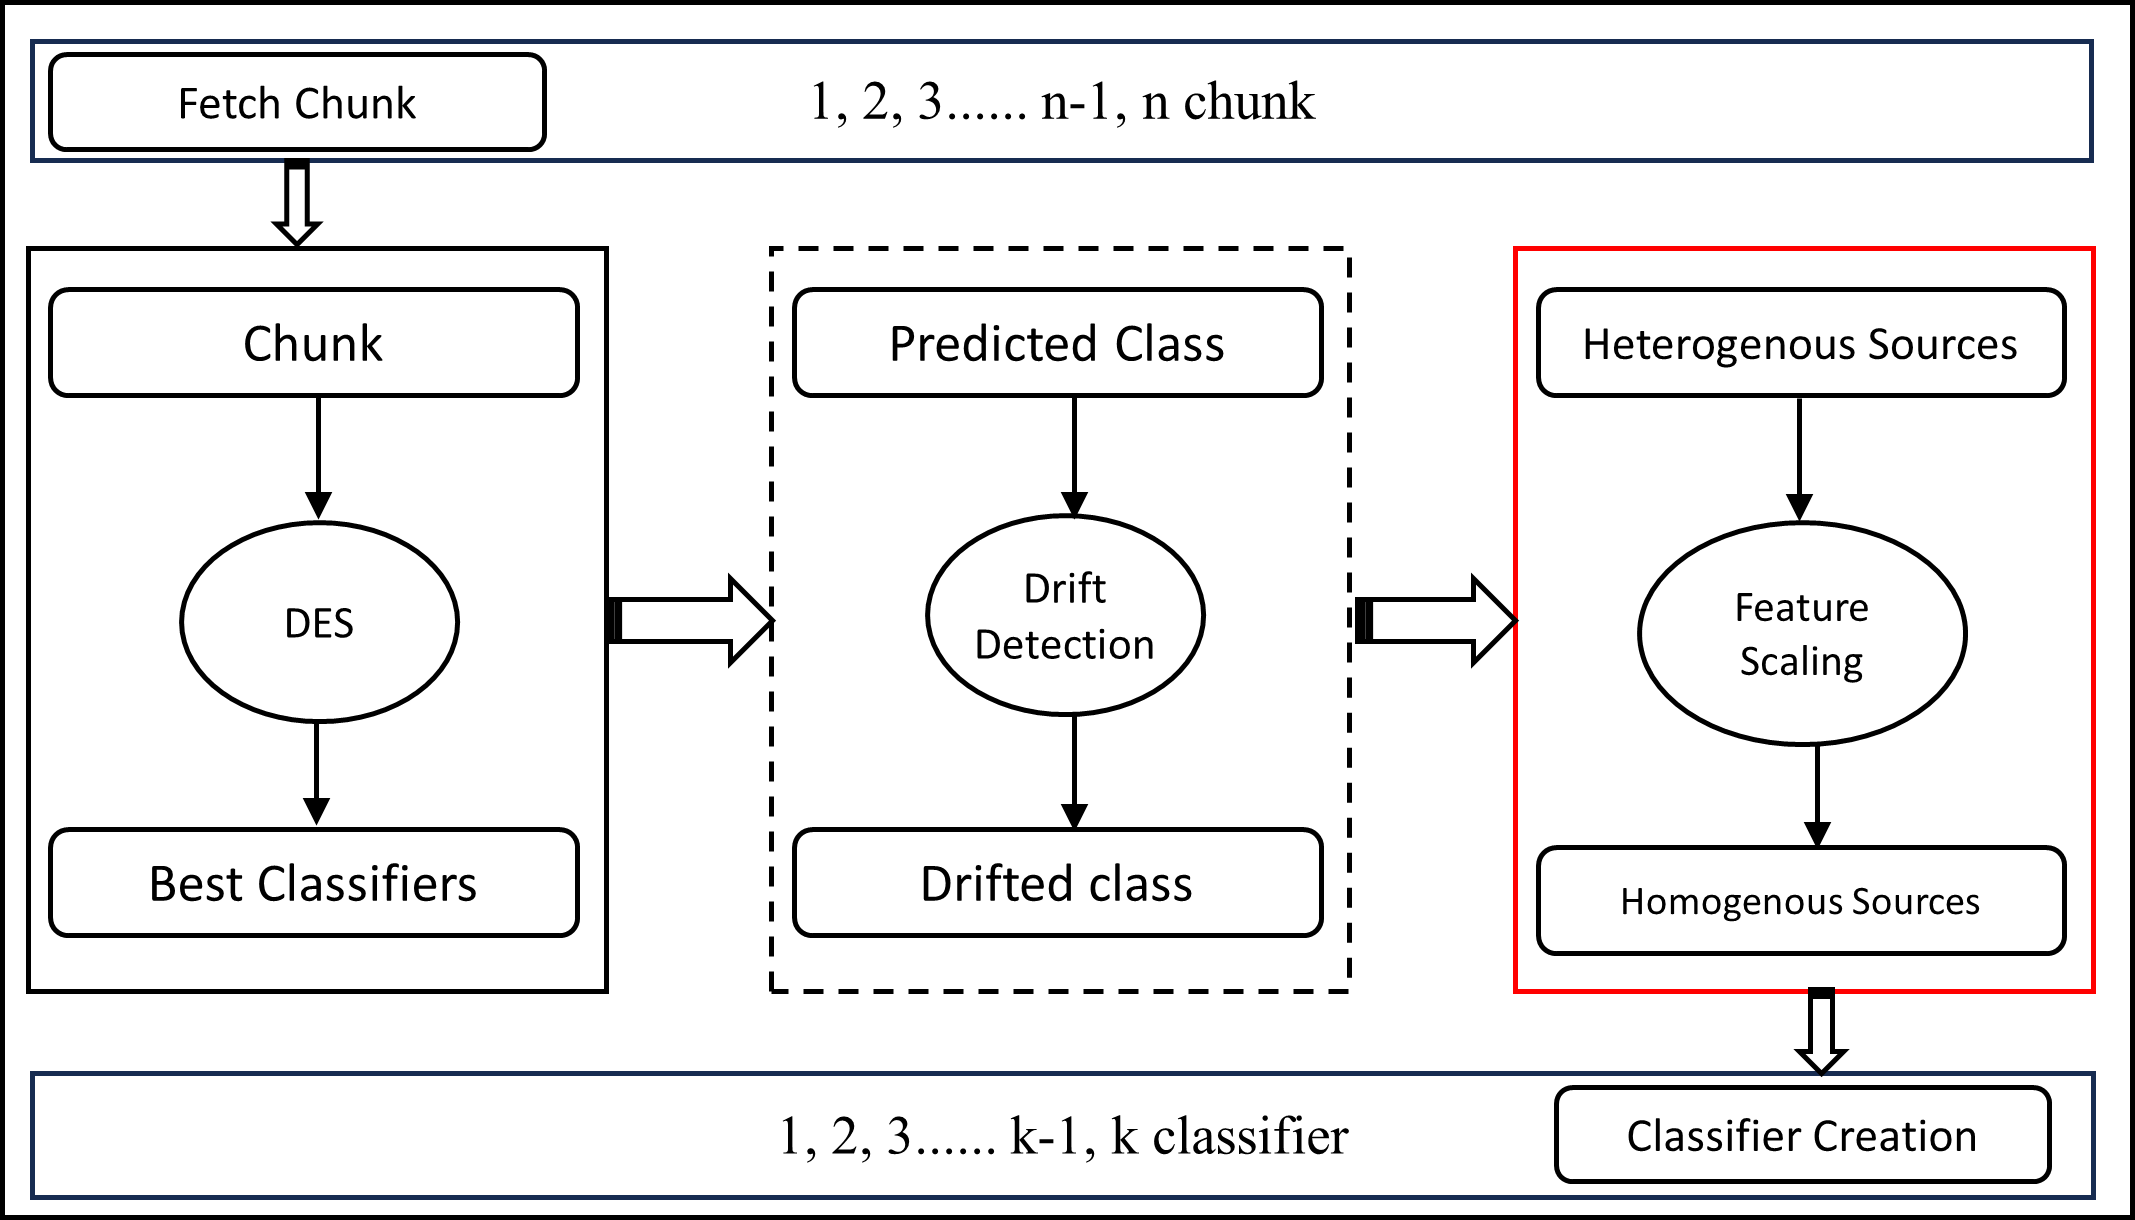
\includegraphics[width=0.85\linewidth]{6_transfer_learning/figures/alg1.png}
	\caption{Heterogeneous Transfer Learning (HTL) Approch Flow.}
	\label{fig:6_alg1}
\end{figure}
\begin{figure}[!ht]
	\centering
	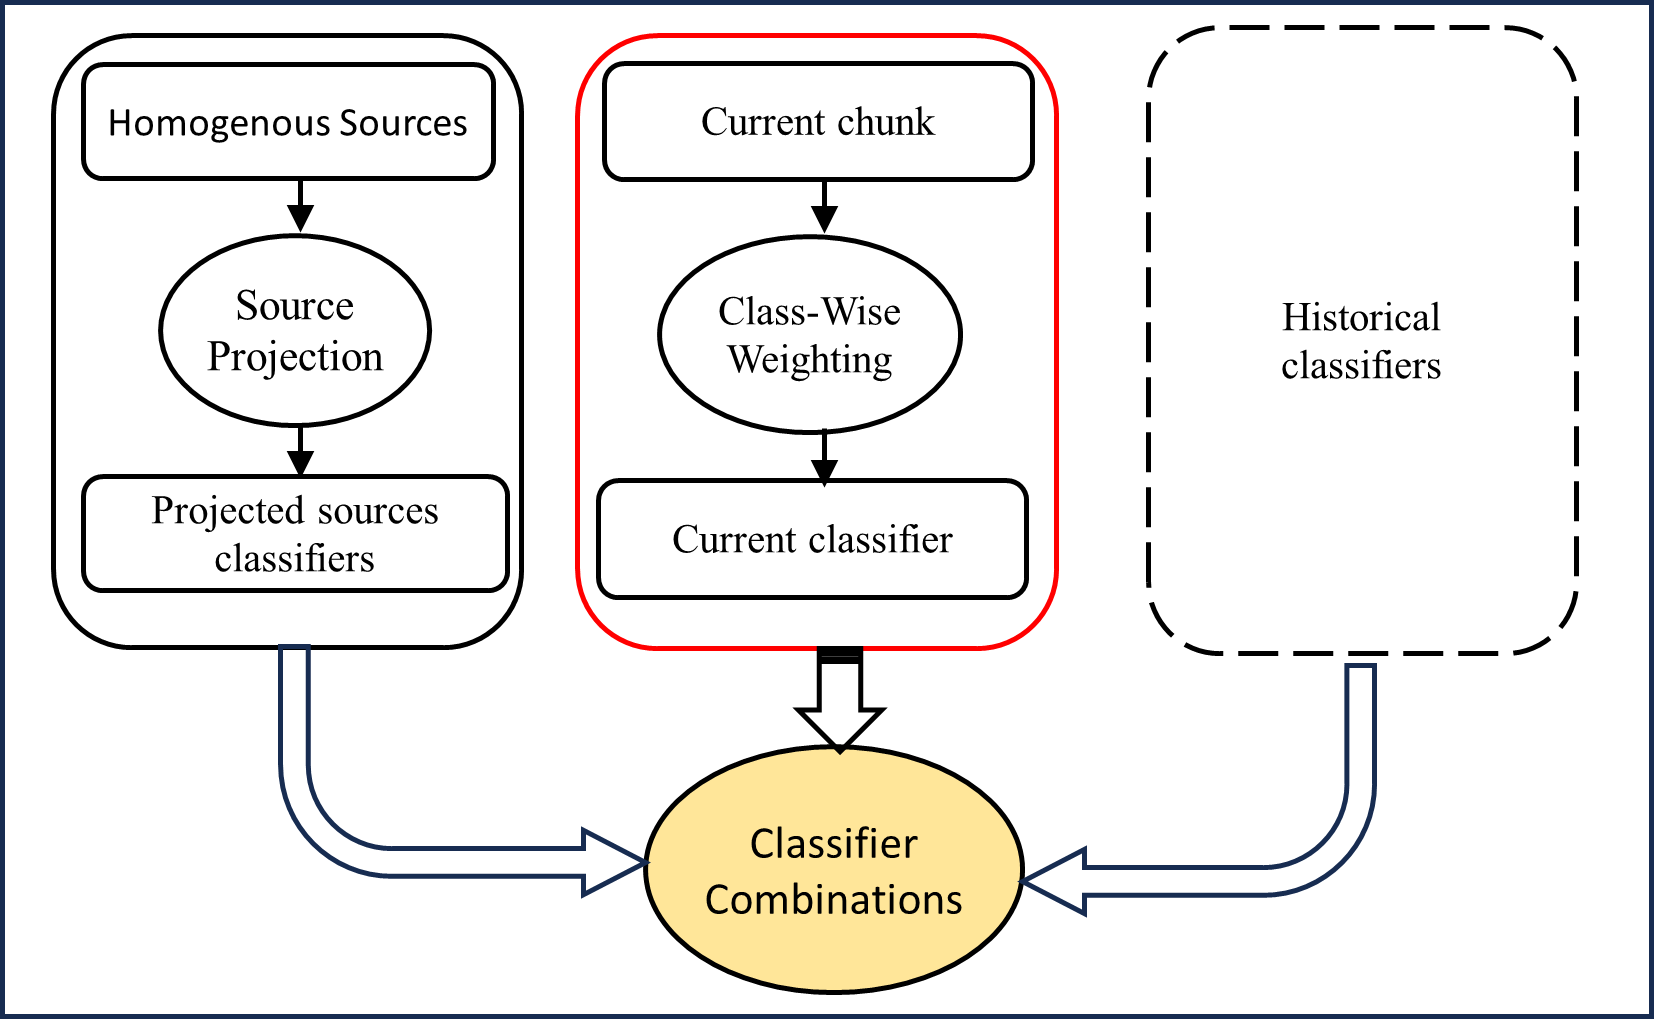
\includegraphics[width=0.85\linewidth]{6_transfer_learning/figures/alg2.png}
	\caption{Approach for Classifier Creation.}
	\label{fig:6_alg2}
\end{figure}

\begin{equation}
	\label{eq:6_eq_1}
	{classWeight}{k,c,\mathcal{D}} = \sum_{i \in \mathcal{D}} \frac{|{prediction}_i = c|}{|\mathcal{D}|} \times \frac{|{prediction}_i \neq c|}{|\mathcal{D}|} \quad
\end{equation}

\begin{equation}
	\label{eq:6_eq_2}
	{classifierWeight} = \sum_{k \in K} \sum_{c \in C} {classWeight}_{k,c,\mathcal{D}} \quad where \mathcal{D} = 1,2,3 \dots N
\end{equation}

\begin{equation}
	\label{eq:6_eq_3}
    {Prediction}_{p,H,k,chunk} = \sum_{p \in P} {{prediction}^{p}_{chunk}} +  \sum_{h \in H} {{prediction}^{h}_{chunk}} + {prediction}^{k}_{chunk}
\end{equation}

\begin{algorithm}[ht]
	\DontPrintSemicolon
	\KwIn{Target domain stream \emph{stream}, heterogeneous multisource domain $\Psi$, pool of classifiers, threshold $\ell$}
		\KwData{Current chunk \emph{a}, classifiers \emph{k}, source classifiers $\psi$, projected source domain \emph{S}, target domain weights $\omega$, source domain weights $\lambda$}
		\KwOut{Prediction}
		  \For{$ \emph{stream}\ have\ chunk$ }{
				  \eIf{$\emph{a}\ is\ the\ First\ chunk$}{
				    $\Psi \gets convertSourcesToTargetDim(\Psi,\ \emph{a})$\;
				    $\emph{k} \gets  trainingNewClassifier(\emph{a})$\;
				    $\lambda \gets SourcesDomainWeights(\Psi,\ \emph{k})$\;
						 $\omega \gets classWiseWeights(\emph{K},\ \emph{a})$\;
				    $\emph{S} \gets projectedSourceDomain(\Psi,\ \lambda)$\;
				   \For{$\emph{source}\ in\ \emph{S}$}{
						 $\emph{newClassifier} \gets  trainingNewClassifier(\emph{source})$\;
				    $\psi \gets  \psi \cup\  \emph{newClassifier}$\;
			  
				   }
				   $\emph{prediction} \gets getPrediction(\emph{a},\ \emph{k},\ \psi,\ \lambda,\ \omega)$ \;
				   }{
				   $\emph{prediction} \gets getPrediction(\emph{a},\ \emph{k},\ \psi)$ \;
					   $driftResult \gets conceptDriftDetector(\emph{prediction})$ \;
			  
					  \If{ $driftResult\ have\ drift $}{
					    $\emph{newClassifier} \gets trainingNewClassifier(\emph{a})$\;
				    $\emph{k} \gets \emph{k}\ \cup \emph{newClassifier}$\;
						\If{$size(\emph{K}) \geq \ell$}{
						 $removeWorstClasssifier(\emph{k})$\;
						}
				    $\lambda \gets SourcesDomainWeights(\Psi,\ \emph{k})$\;
				    $\omega \gets classWiseWeights(\emph{K},\ \emph{a})$\;
			  
				    $\emph{S} \gets projectedSourceDomain(\Psi,\ \lambda)$\;
				   \For{$\emph{source}\ in\ \emph{S}$}{
						 $\emph{newClassifier} \gets  trainingNewClassifier(\emph{source})$\;
				    $\psi \gets  \psi \cup\  \emph{newClassifier}$\;
			  
				   }
				  
				   $\emph{prediction} \gets getPrediction(\emph{a},\ \emph{k},\ \psi,\ \lambda,\ \omega)$ \;
					 }
				  }
				  }
	\Return{$\emph{prediction}$}\;
	\caption{Flow of the Heterogeneous Transfer Learning (HTL).}
	\label{alg:6_alg_1}

\end{algorithm}


\section{Experimental Results}
\label{sec:6_Expsetup}

In this section, the proposed HTL, CORAL \cite{sun2016return}, and CDTL \cite{yang2021concept}, and Melanie \cite{dong2019multistream} algorithms are compared. Three subsections are introduced: the first section focuses on the experimental setup; second, a discussion on data streams to apply all experiments on heterogeneous and homogeneous source domains, including a comparison to evaluate the runtime factor between all methods; and finally, a comparison is made between online learning and chunk-based concept drift.
\subsection{Experimental setup}
The evaluation of Heterogeneous Taxonomy Learning (HTL) involves a comparison with CORAL \cite{sun2016return}, CDTL \cite{yang2021concept}, and Melanie \cite{dong2019multistream}  which employs multiple metrics such as precision, recall, $f_1$ score \cite{sasaki2007truth}, BAC \cite{brodersen2010balanced}, and G-mean \cite{kubat1997addressing}. The experimental protocol employed for evaluation followed the test-then-train approach \cite{krawczyk2017ensemble}, where the classification model is trained on a specific data chunk and subsequently evaluated on the next chunk. The chunk size was standardized to 2000 instances. Four different classification models were used as base estimators: k-Neighbors (KNN) algorithm, Support Vector Machine (abbreviated as SVM), Gaussian Naive Bayes abbreviated as (GNB), and Hoeffding Tree (abbreviated as HT), as implemented in scikit-learn \cite{frias2014online}. We establish an ensemble classifier pool with a set limit of $L$ = 8, wherein each ensemble consists of $N$ = 4 base models. While these constraints remained fixed across all experiments, the threshold for the pool classifier in each approach was maintained at eight. Consequently, if the threshold is surpassed, the least-performing classifier is systematically eliminated. This configuration was applied consistently across all approaches to ensure fair engagement. The experiments were carried out using the Python programming language, with the source code publicly accessible on GitHub\footnote{\url{https://github.com/Amadkour/transfer_learning_with_concept_drift.git}} . When dealing with heterogeneous multisource streams, it is often impractical or not applicable to truly heterogeneous experiences. Consequently, the eigenvector technique was utilized in all related approaches. This decision stems from the fact that the algorithms in related work primarily focus on homogeneous source domains and do not address the challenges posed by heterogeneous multisource data. Therefore, heterogeneous experiments were conducted.

\subsubsection{Data Streams}
In this study, the performance of the third proposed approach was evaluated using various datasets, including synthetic data streams, a real application stream, and dataset benchmark datasets. To conduct the evaluations, the stream-learn Python library \cite{ksieniewicz2022stream,madkour2023historical} was used. As detailed in Table 1, the benchmark dataset employed in the study is the Covertype dataset. This dataset comprises 52 features, 7 classes, and a total of 581,010 instances. It serves as a standard benchmark dataset widely used in stream mining research. For the evaluation of real application streams, the Sensor Stream dataset was utilized. This dataset includes 5 features, 58 classes, and a total of 392,600 instances, representing a real-world application scenario. Synthetic datasets were generated using the scikit-learn Python package. This synthetic dataset was created to simulate data streams and evaluate the performance of the framework. The synthetic datasets consisted of 10 features and four classes and were divided into 200 chunks. Each chunk had a size of 2,000. The performance of the third proposed approach was systematically evaluated using these datasets and a stream-learn library. These evaluations provided valuable insights into the effectiveness of the framework in handling different types of data streams, including benchmark datasets, real application streams, and synthetic data streams.

\begin{table}[H]
  \centering
  \caption{Summary of Dataset Characteristics Utilized in the HTL.}
  \resizebox{\textwidth}{!}{
  \begin{tabular}{|l|c|c|c|}
  \hline
  \textbf{Dataset} & \textbf{Number of Features} & \textbf{Number of Classes} & \textbf{Number of Instances} \\ \hline
  Covertype dataset\footnote{\url{http://archive.ics.uci.edu/dataset/31/covertype}} & 40 & 7 & 581,010 \\ \hline
  Sensor Stream dataset\footnote{\url{https://www.cse.fau.edu/~xqzhu/Stream/sensor.arff}} & 5 & 58 & 392,600 \\ \hline
  Synthetic stream-52 & 52 & 5 & 200,000 \\ \hline
  Synthetic stream-8 & 8 & 4 & 200,000 \\ \hline
  \end{tabular}
  }
  \label{table:6_table1}
  \end{table}

  \subsubsection{Compared Approaches}
  In the subsequent section,the established benchmark techniques is introduced as outlined below:
  \begin{itemize}
    \item \textbf{AW-CORAL \cite{sun2016return}:} The AW- CORAL (Adaptive Weighted CORrelation ALignment) method is a simple domain adaptation technique designed to align the distributions of both source and target features without supervision. This is accomplished by aligning second-order statistics, focusing specifically on covariance, to match the distributions between the domains.
    \item \textbf{HE-CDTL \cite{sun2016return}:} The HE-CDTL approach tackles Concept Drift Transfer Learning (CDTL) by integrating knowledge from source domains and historical time steps in the target domain to improve learning performance. HE-CDTL features class-wise weighted ensemble for independent selection of historical knowledge by each class, and AW-CORAL to mitigate domain discrepancy and reduce negative knowledge transfer.
    \item \textbf{Melanie \cite{dong2019multistream}:} Multisource Online Transfer Learning for Non-stationary Environments, known as Melanie, represents the inaugural method capable of transferring knowledge across various data streaming sources in non-stationary environments. Melanie constructs numerous sub-classifiers to grasp diverse facets from distinct source and target concepts dynamically. It identifies sub-classifiers that align closely with the prevailing target concept, assembling them into an ensemble for predicting instances originating from the target concept.
  \end{itemize}

While Melanie extends online learning through chunk-based learning akin to CDTL, it exhibits two limitations: 
\begin{itemize}
  \item utilizing a global weight for each classifier, disregarding performance variation across different locations of a data chunk
  \item combining learned classifiers from these domains directly with the target classifier, which may impede effective knowledge transfer due to domain discrepancies. Hence, the third proposed approach (HTL) is compared with AW- CORAL \cite{sun2016return} and HE-CDTL \cite{yang2021concept}.
\end{itemize}

\subsection{Analysis of Experimental Results}

This section evaluates the proposed approach's performance across multiple data streams using five metrics: $f_1$ score, precision, recall, G-mean, and BAG. Two visualization techniques, radar and line diagrams, were employed. Radar charts summarized algorithm performance across metrics, while line diagrams focused on G-mean comparisons across 100 chunks. The first five experiments used line diagrams, and the last two combined radar and line charts, offering a detailed evaluation of the third proposed approach under diverse scenarios.

\subsubsection{Results on Target Domains Dataset without Source Domain}
Figure \ref{fig:6_exp1} presents the results of applying various classification methods to the Covertype dataset without employing a source domain stream. The line diagram reveals the classification performance, assessed using the G-mean metric, over 100 data chunks for each method. Philosophically, the observed trajectory of performance reflects an epistemological journey from initial uncertainty to eventual refinement and adaptation. The suboptimal performance during the initial 10 chunks suggests a nascent phase where the system's understanding is limited, akin to the formative stages of knowledge acquisition. This phase is marked by an incomplete pool of classifiers, signifying the constraints of limited epistemic resources. As the classifier pool expands, representing an enrichment of the system’s cognitive tools, the DES technique demonstrates an enhanced ability to discern and apply the most suitable classifier for each incoming data chunk. This mirrors the philosophical principle of cumulative epistemic progress, where successive integration of knowledge resources fosters improved understanding and capability. Between chunk 20 and the final chunk, HTL consistently outperforms other methods. This superiority is attributable to its weighting mechanism, which assigns significance to historical classifiers, embodying a philosophical stance that values historical precedent and contextual relevance in constructing present knowledge. The ability of HTL to effectively leverage this weighting method facilitates the training of the classifier pool, thereby amplifying its overall efficacy.  
In contrast, the variable performance of CORAL and CDTL in certain chunks highlights the inherent challenges of reconciling differing approaches to knowledge adaptation. This variability underscores the dynamic interplay of methodologies, each striving to balance generality and specificity in their engagement with a continually evolving data stream.
\begin{figure}[H]
	\centering
	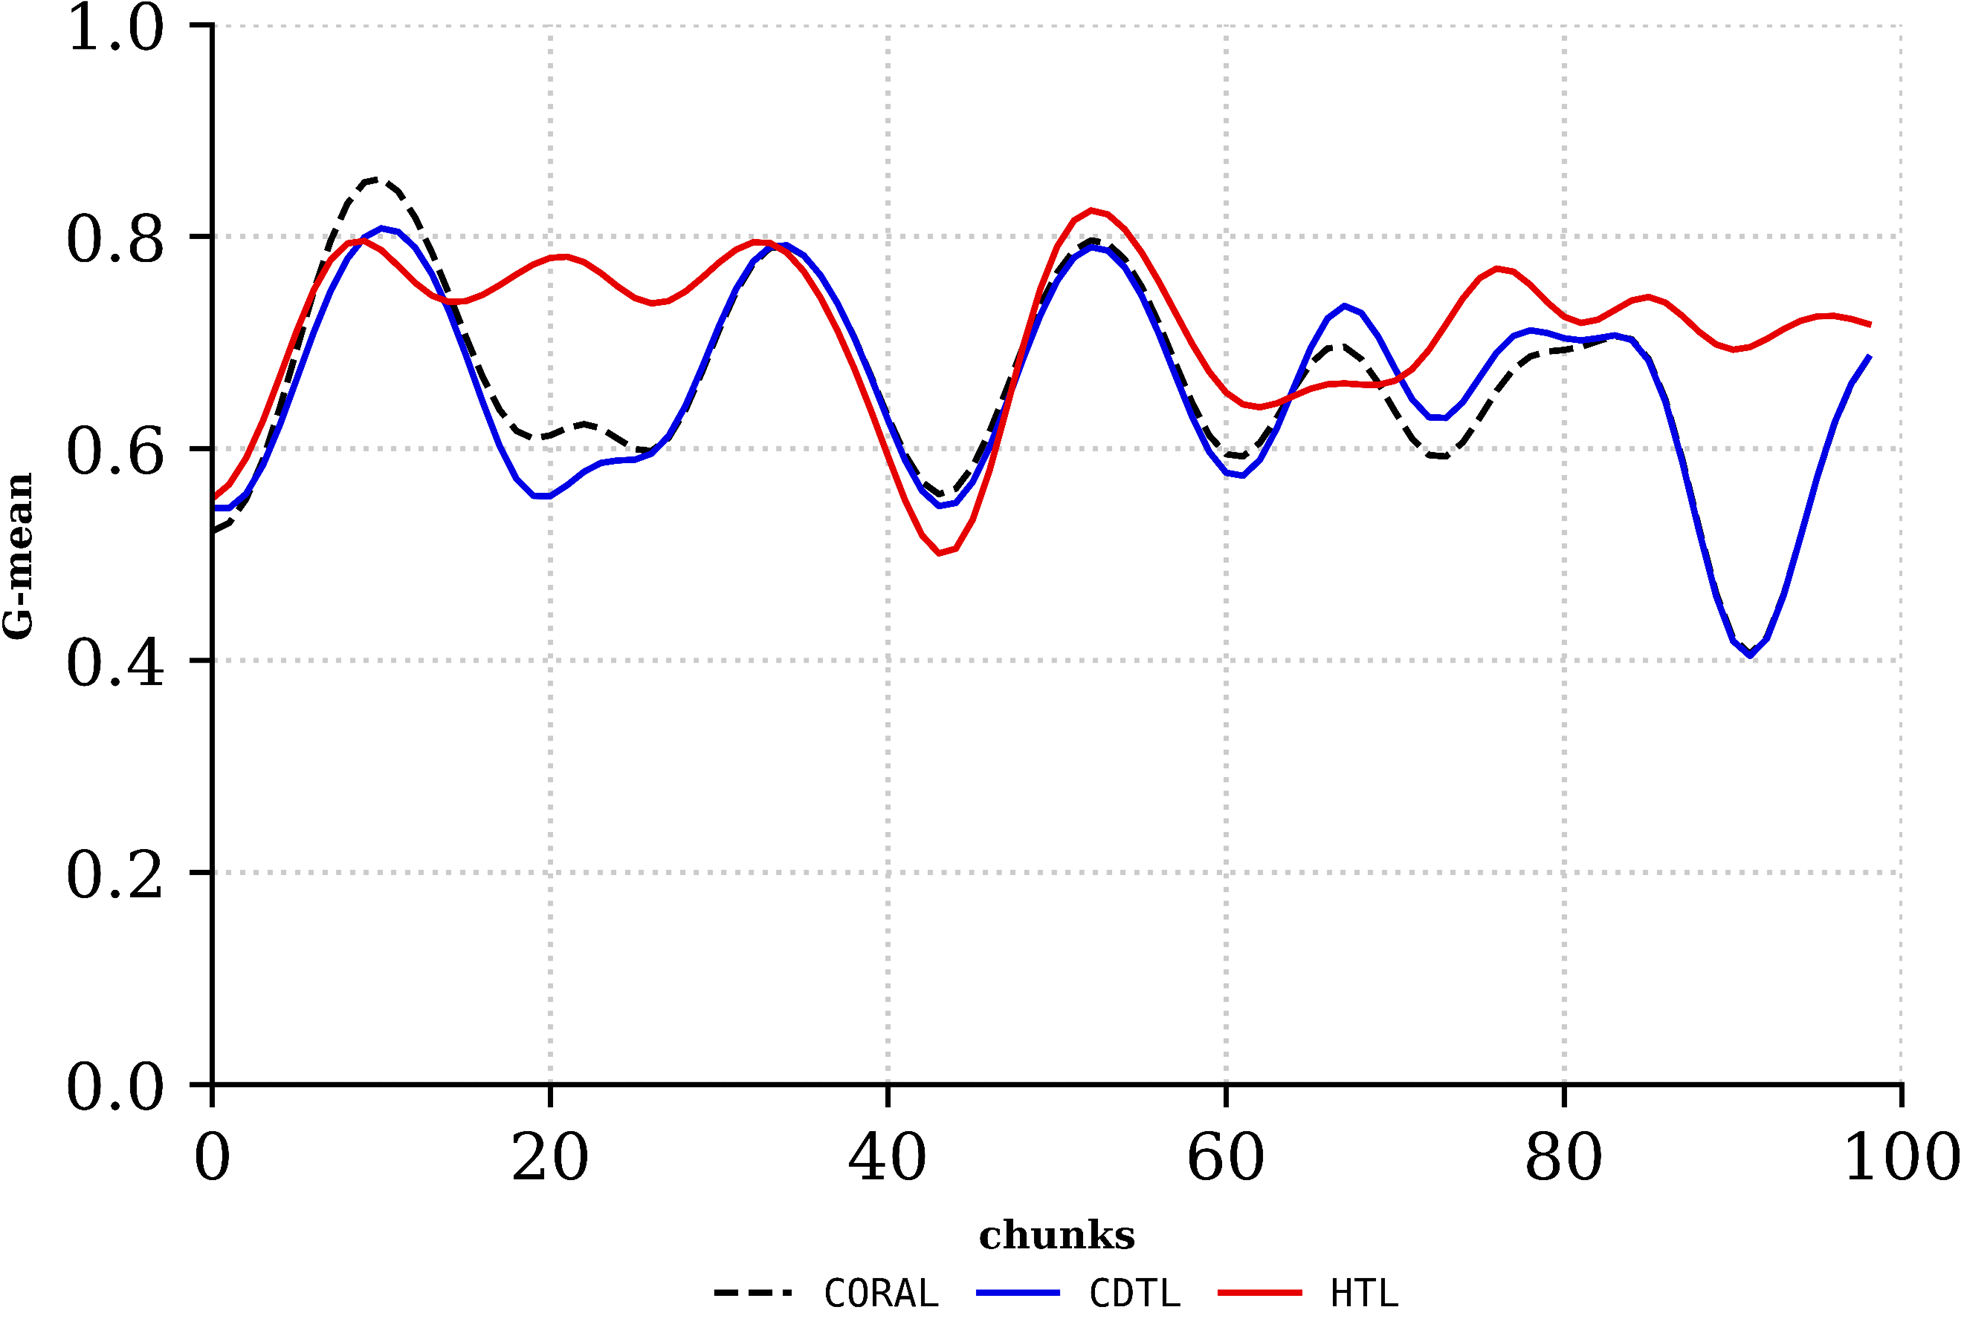
\includegraphics[width=0.6\linewidth]{6_transfer_learning/figures/exp1_0.png}
  \caption{Results of the Covertype Stream as the Target Domain without the Source Domain.}

	\label{fig:6_exp1}
\end{figure}
\begin{figure}[H]
	\centering
	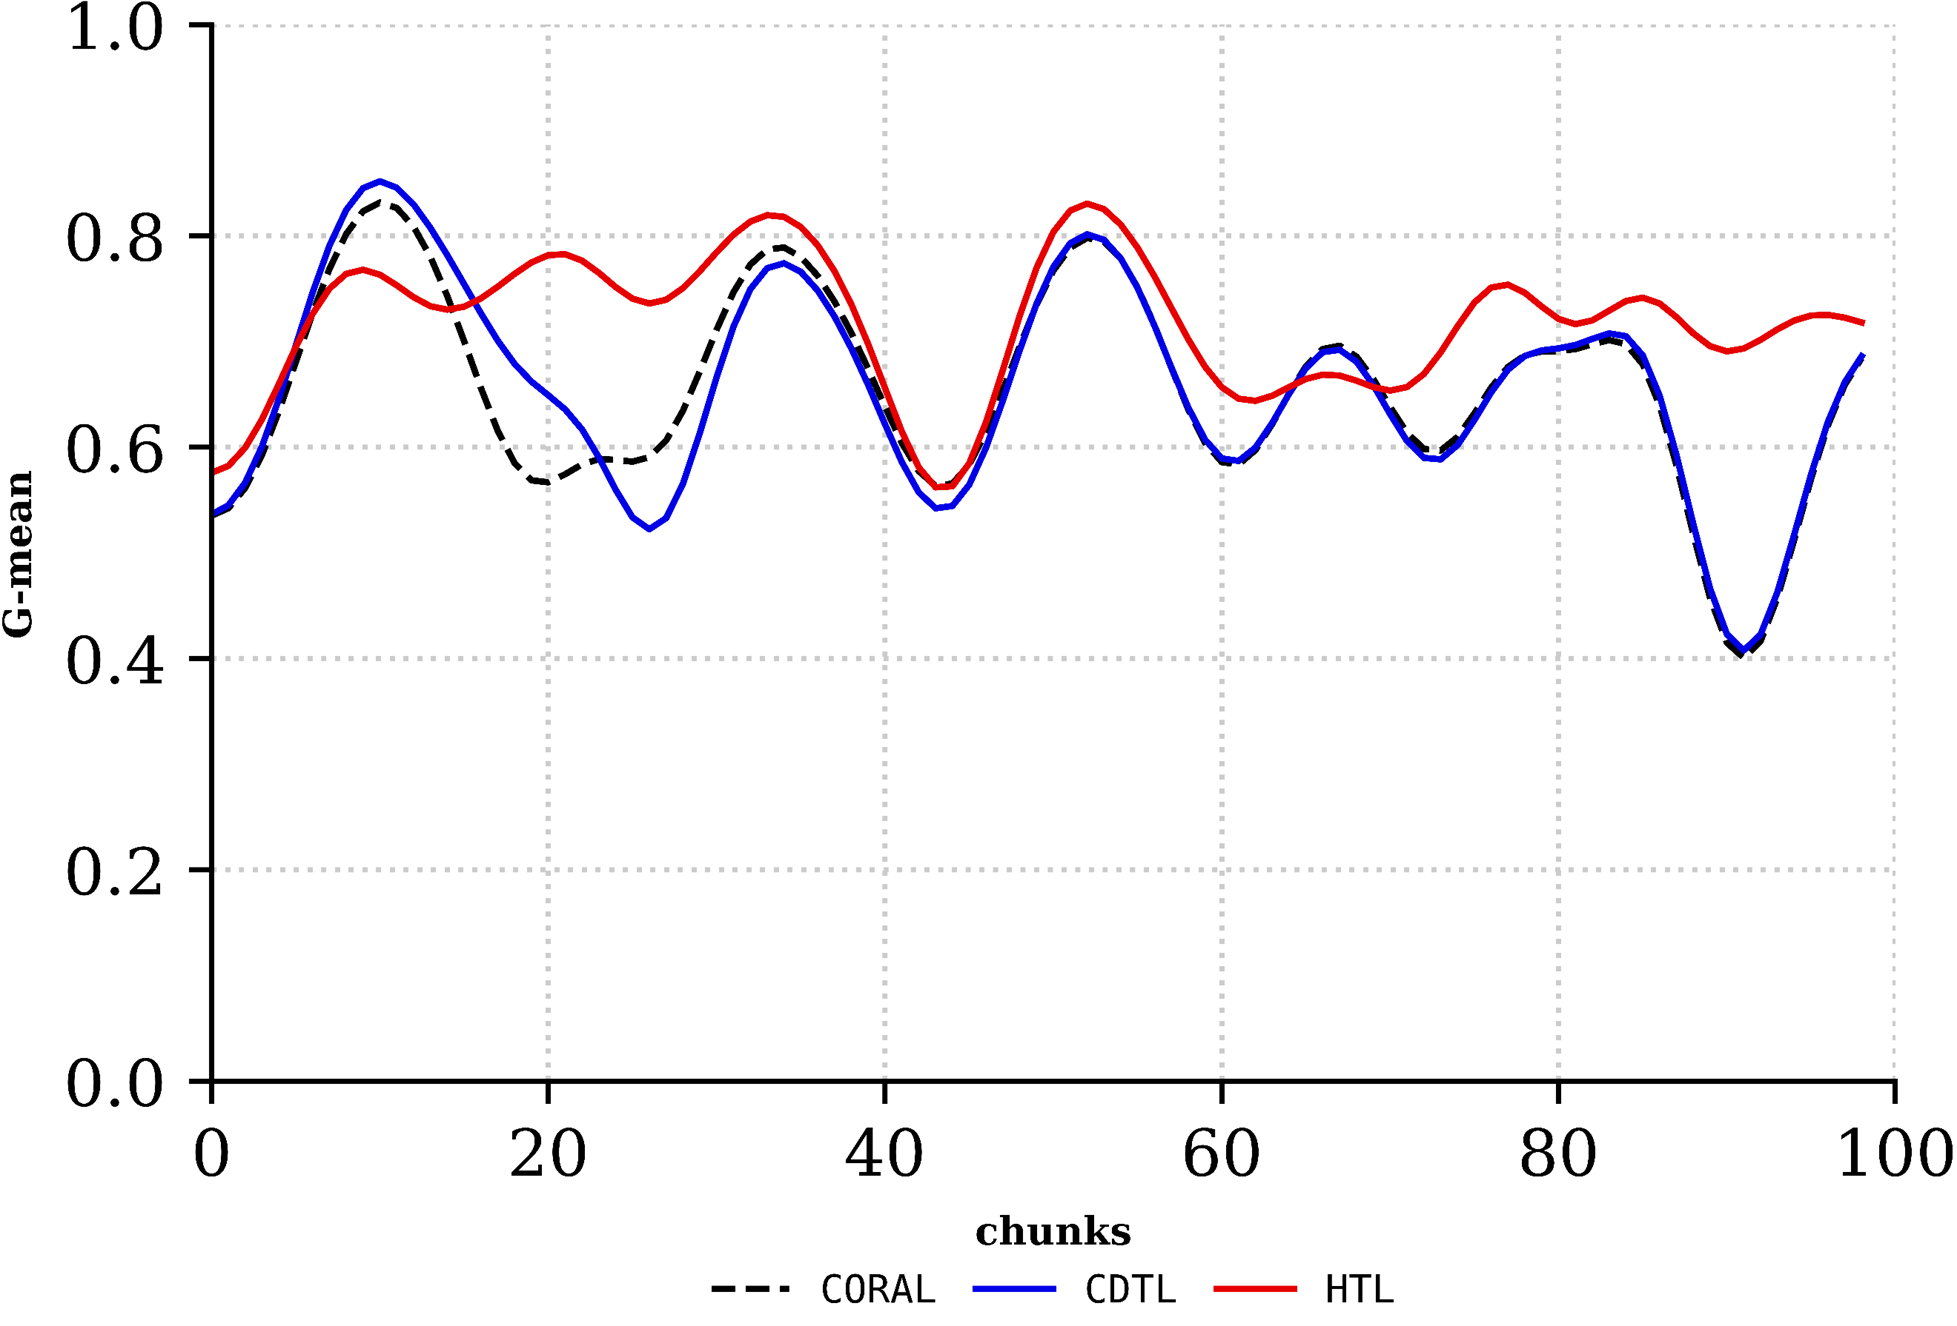
\includegraphics[width=0.6\linewidth]{6_transfer_learning/figures/exp1_1.png}
	\caption{Performance results of the Covertype Stream as the target domain using homogeneous source domains.}

	\label{fig:6_exp2}
\end{figure}

\subsubsection{Results on the Homogeneous Source Domains Dataset}
Figure \ref{fig:6_exp2} illustrates the outcomes of applying the compared methods to the Covertype data stream as a target domain, with Synthetic-52 serving as a homogenous source domain. This scenario introduces an epistemological dimension rooted in the interaction between prior knowledge (the source domain) and newly encountered contexts (the target domain). The line diagram reveals HTL’s initially suboptimal performance across the first eight chunks, attributable to the limited pool of classifiers available in the early phase. This aligns with the philosophical notion of an incomplete epistemic framework, where insufficient resources impede initial understanding. As the classifier pool expands beyond the eighth chunk, HTL’s performance improves, underscoring the significance of cumulative resource enrichment in advancing predictive accuracy. CDTL maintains consistent performance throughout the chunks, reflecting an equilibrium-based adaptation strategy that prioritizes stability over dynamic optimization. Meanwhile, CORAL’s consistently lower performance highlights the potential limitations of certain methodologies in transferring knowledge effectively across domains, pointing to the philosophical challenge of achieving universality in adaptive systems.  

Notably, HTL achieves the highest performance across all chunks, emphasizing the utility of its weighting mechanism and its capacity to harness the source domain knowledge effectively. The superior performance of both CDTL and HTL in Figure \ref{fig:6_exp2} compared to Figure \ref{fig:6_exp1} reflects the epistemological advantage conferred by incorporating Synthetic-52 as a source domain. This source-target synergy illustrates the philosophical principle of grounded learning, where external, homogenous knowledge sources enhance the capacity to navigate and adapt to complex, evolving data streams.  

The contrasting scenarios in Figures \ref{fig:6_exp1} and \ref{fig:6_exp2} underscore the critical role of prior knowledge in shaping learning trajectories. In the absence of a source domain, as in Figure \ref{fig:6_exp1}, the methods must independently construct their epistemic framework, leading to comparatively constrained performance. Conversely, the inclusion of a source domain, as shown in Figure \ref{fig:6_exp2}, facilitates a richer epistemic interplay, enhancing adaptability and robustness in the face of dynamic data challenges.


\subsubsection{Results on One Heterogeneous Source Domain}
\begin{figure}[H]
	\centering
	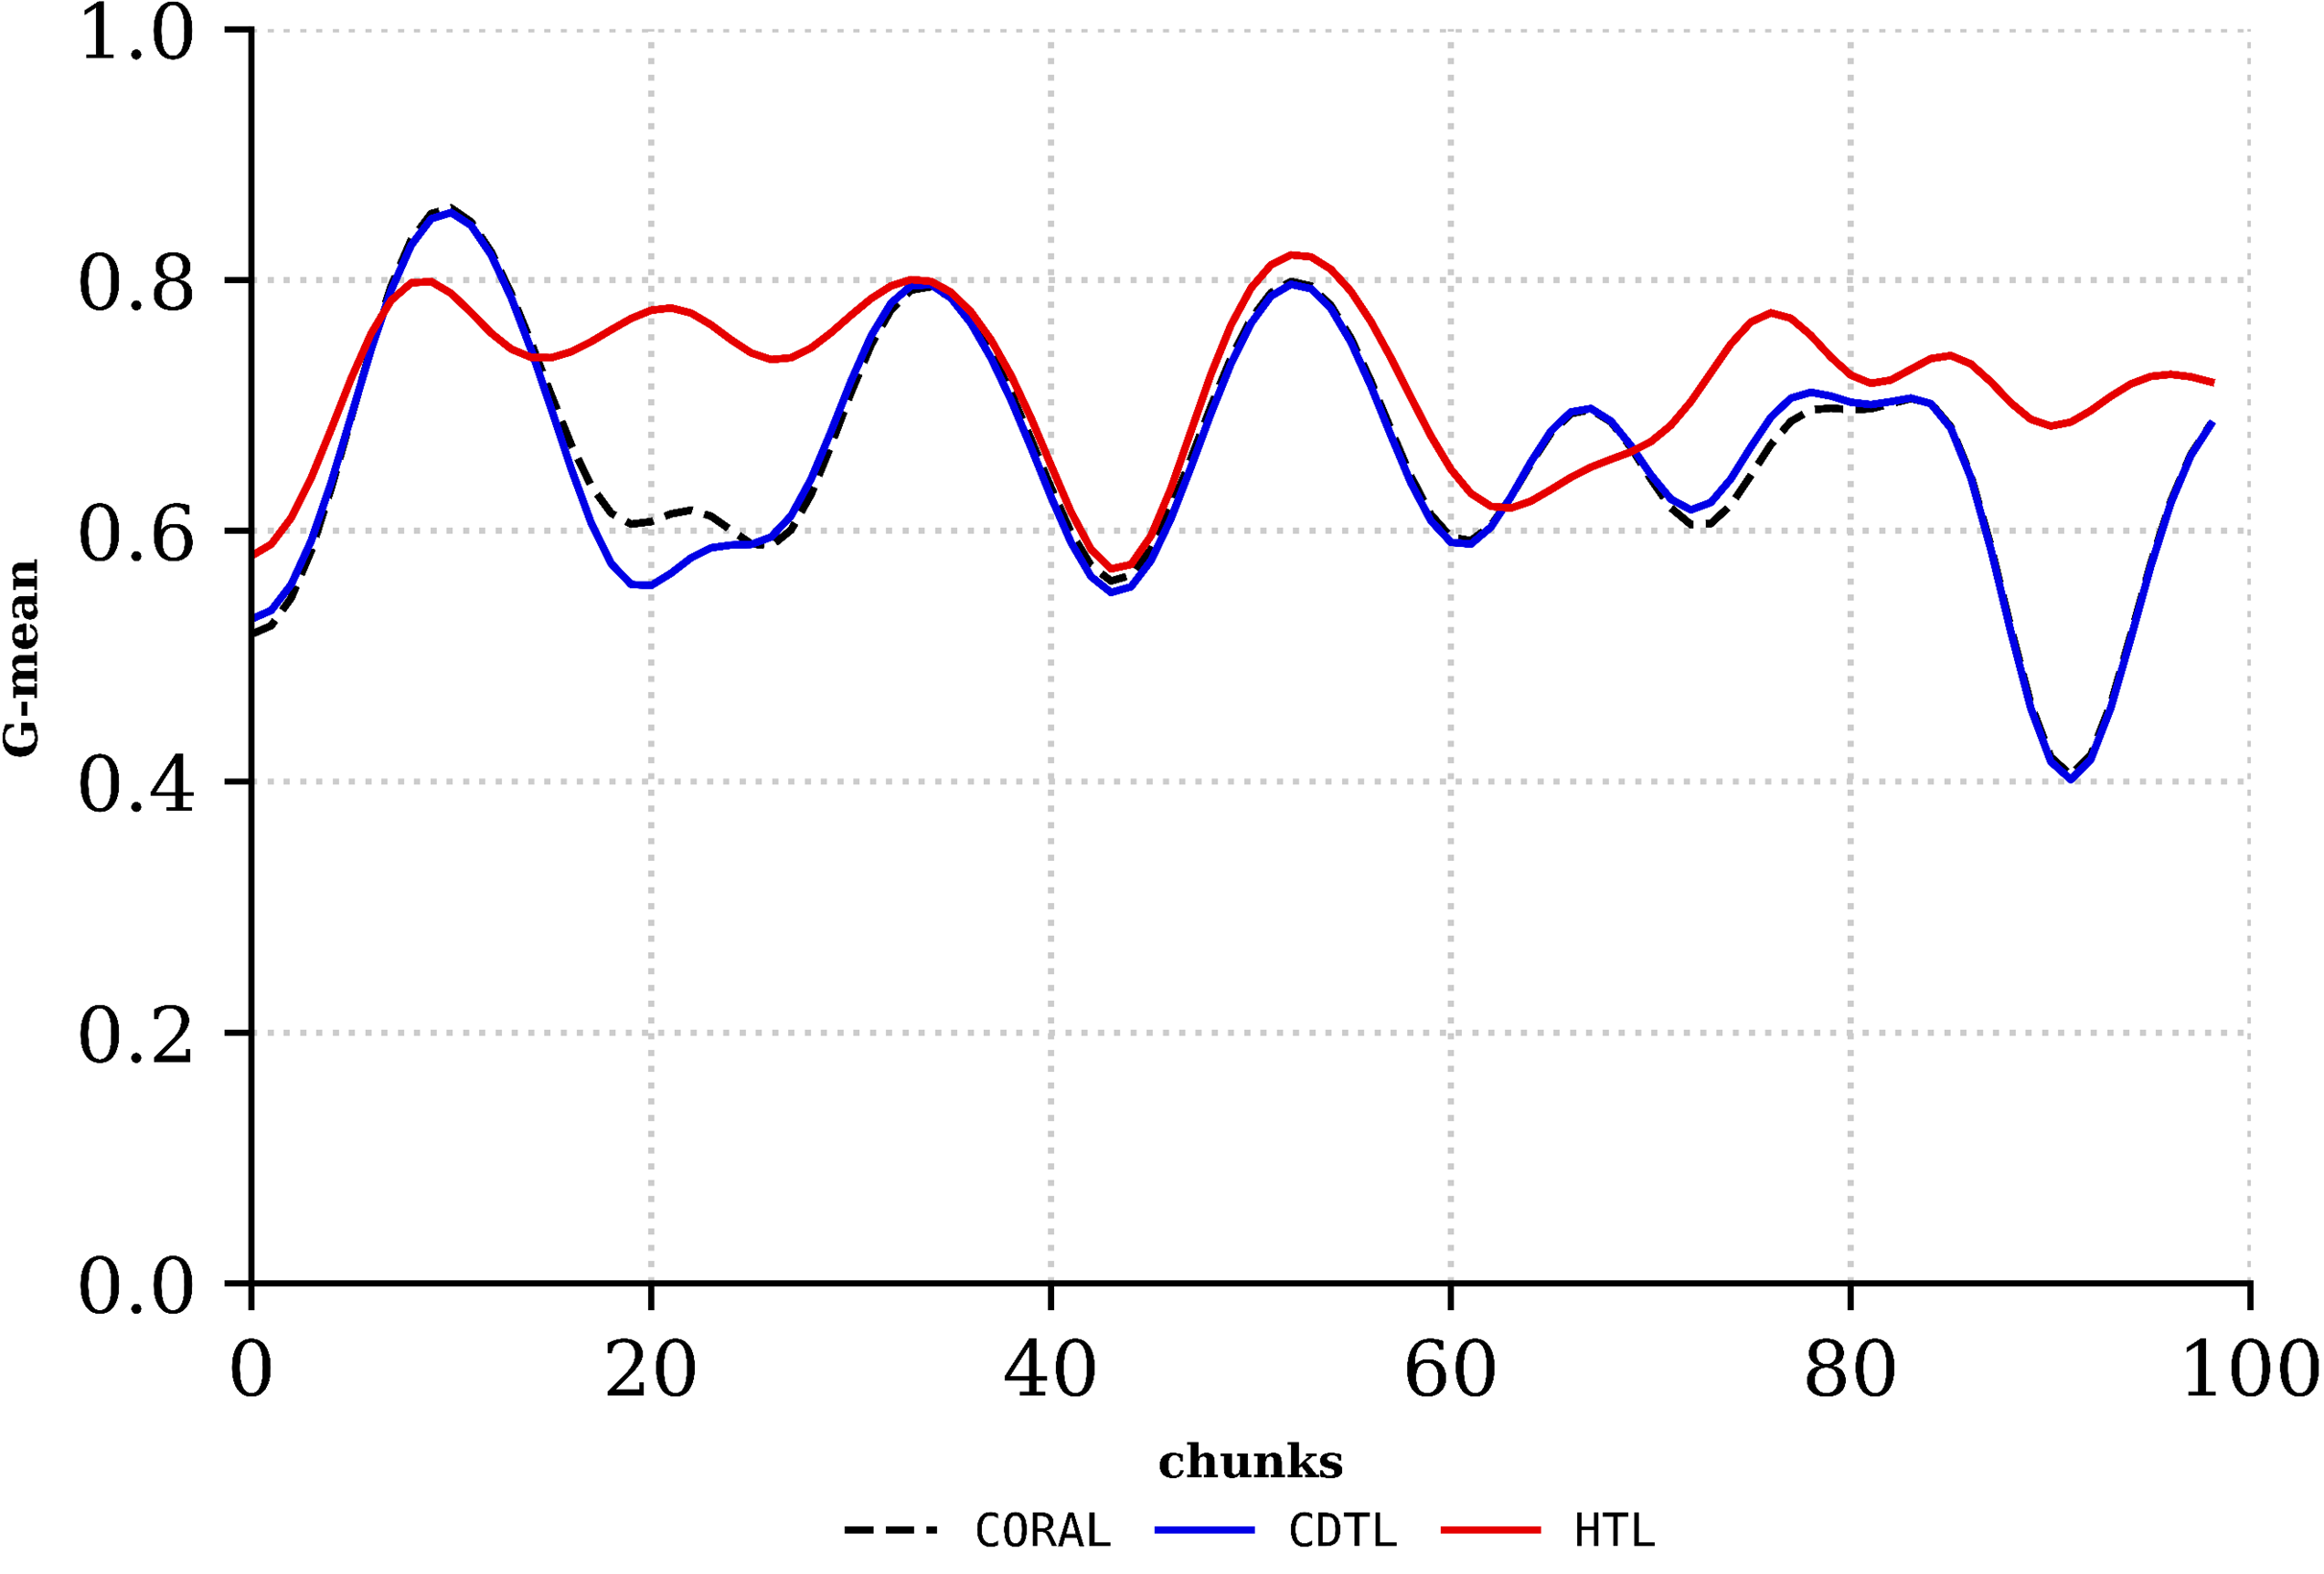
\includegraphics[width=0.6\linewidth]{6_transfer_learning/figures/exp2_0.png}
  \caption{Performance results of the Covertype Stream as the target domain with a single heterogeneous source domain.}

	\label{fig:6_exp3}
\end{figure}
Figure \ref{fig:6_exp3} presents the results of applying the compared methods to the Covertype data stream as the target domain, with Synthetic-8 as a heterogeneous source domain. This experiment explores the epistemological dynamics of knowledge transfer across domains with differing structures, reflecting the philosophical challenges of reconciling heterogeneity in adaptive systems. The Synthetic-8 stream, with its distinct dimensionality (eight features and four classes), contrasts with the Covertype stream. While HTL is inherently designed to handle heterogeneous sources, specific adjustments, such as the application of the eigenvector technique, were required to enable CORAL and CDTL to operate within this domain. This adaptation highlights the importance of methodological flexibility in addressing epistemic diversity and bridging structural disparities between domains.  
The line diagram demonstrates variability in the performance of the approaches across chunks, suggesting that the contribution of the source domain's knowledge is contingent on its alignment with the target domain’s requirements. HTL consistently achieves superior performance across almost all chunks, emphasizing its robust capacity for extracting and applying positive knowledge from heterogeneous sources. This superior adaptability reflects a philosophical commitment to leveraging epistemic pluralism, where diverse knowledge sources enrich the learning system’s overall efficacy.  

In contrast, the comparatively lower performance of CORAL and CDTL underscores the inherent challenges these methods face when transferring knowledge across domains with significant structural differences. The need for eigenvector-based adjustments further emphasizes their limited native capacity for heterogeneous adaptation, revealing the philosophical tension between static methodologies and dynamic, cross-domain requirements. This experiment exemplifies the critical role of epistemological adaptability in heterogeneous environments. The consistent success of HTL underscores the potential of methodologies that embrace diversity in knowledge sources, whereas the relative struggles of CORAL and CDTL highlight the constraints of approaches rooted in homogeneity.

\subsubsection{Results on All Heterogeneous and Covertype as the Target Domain}
\begin{figure}[H]
	\centering
	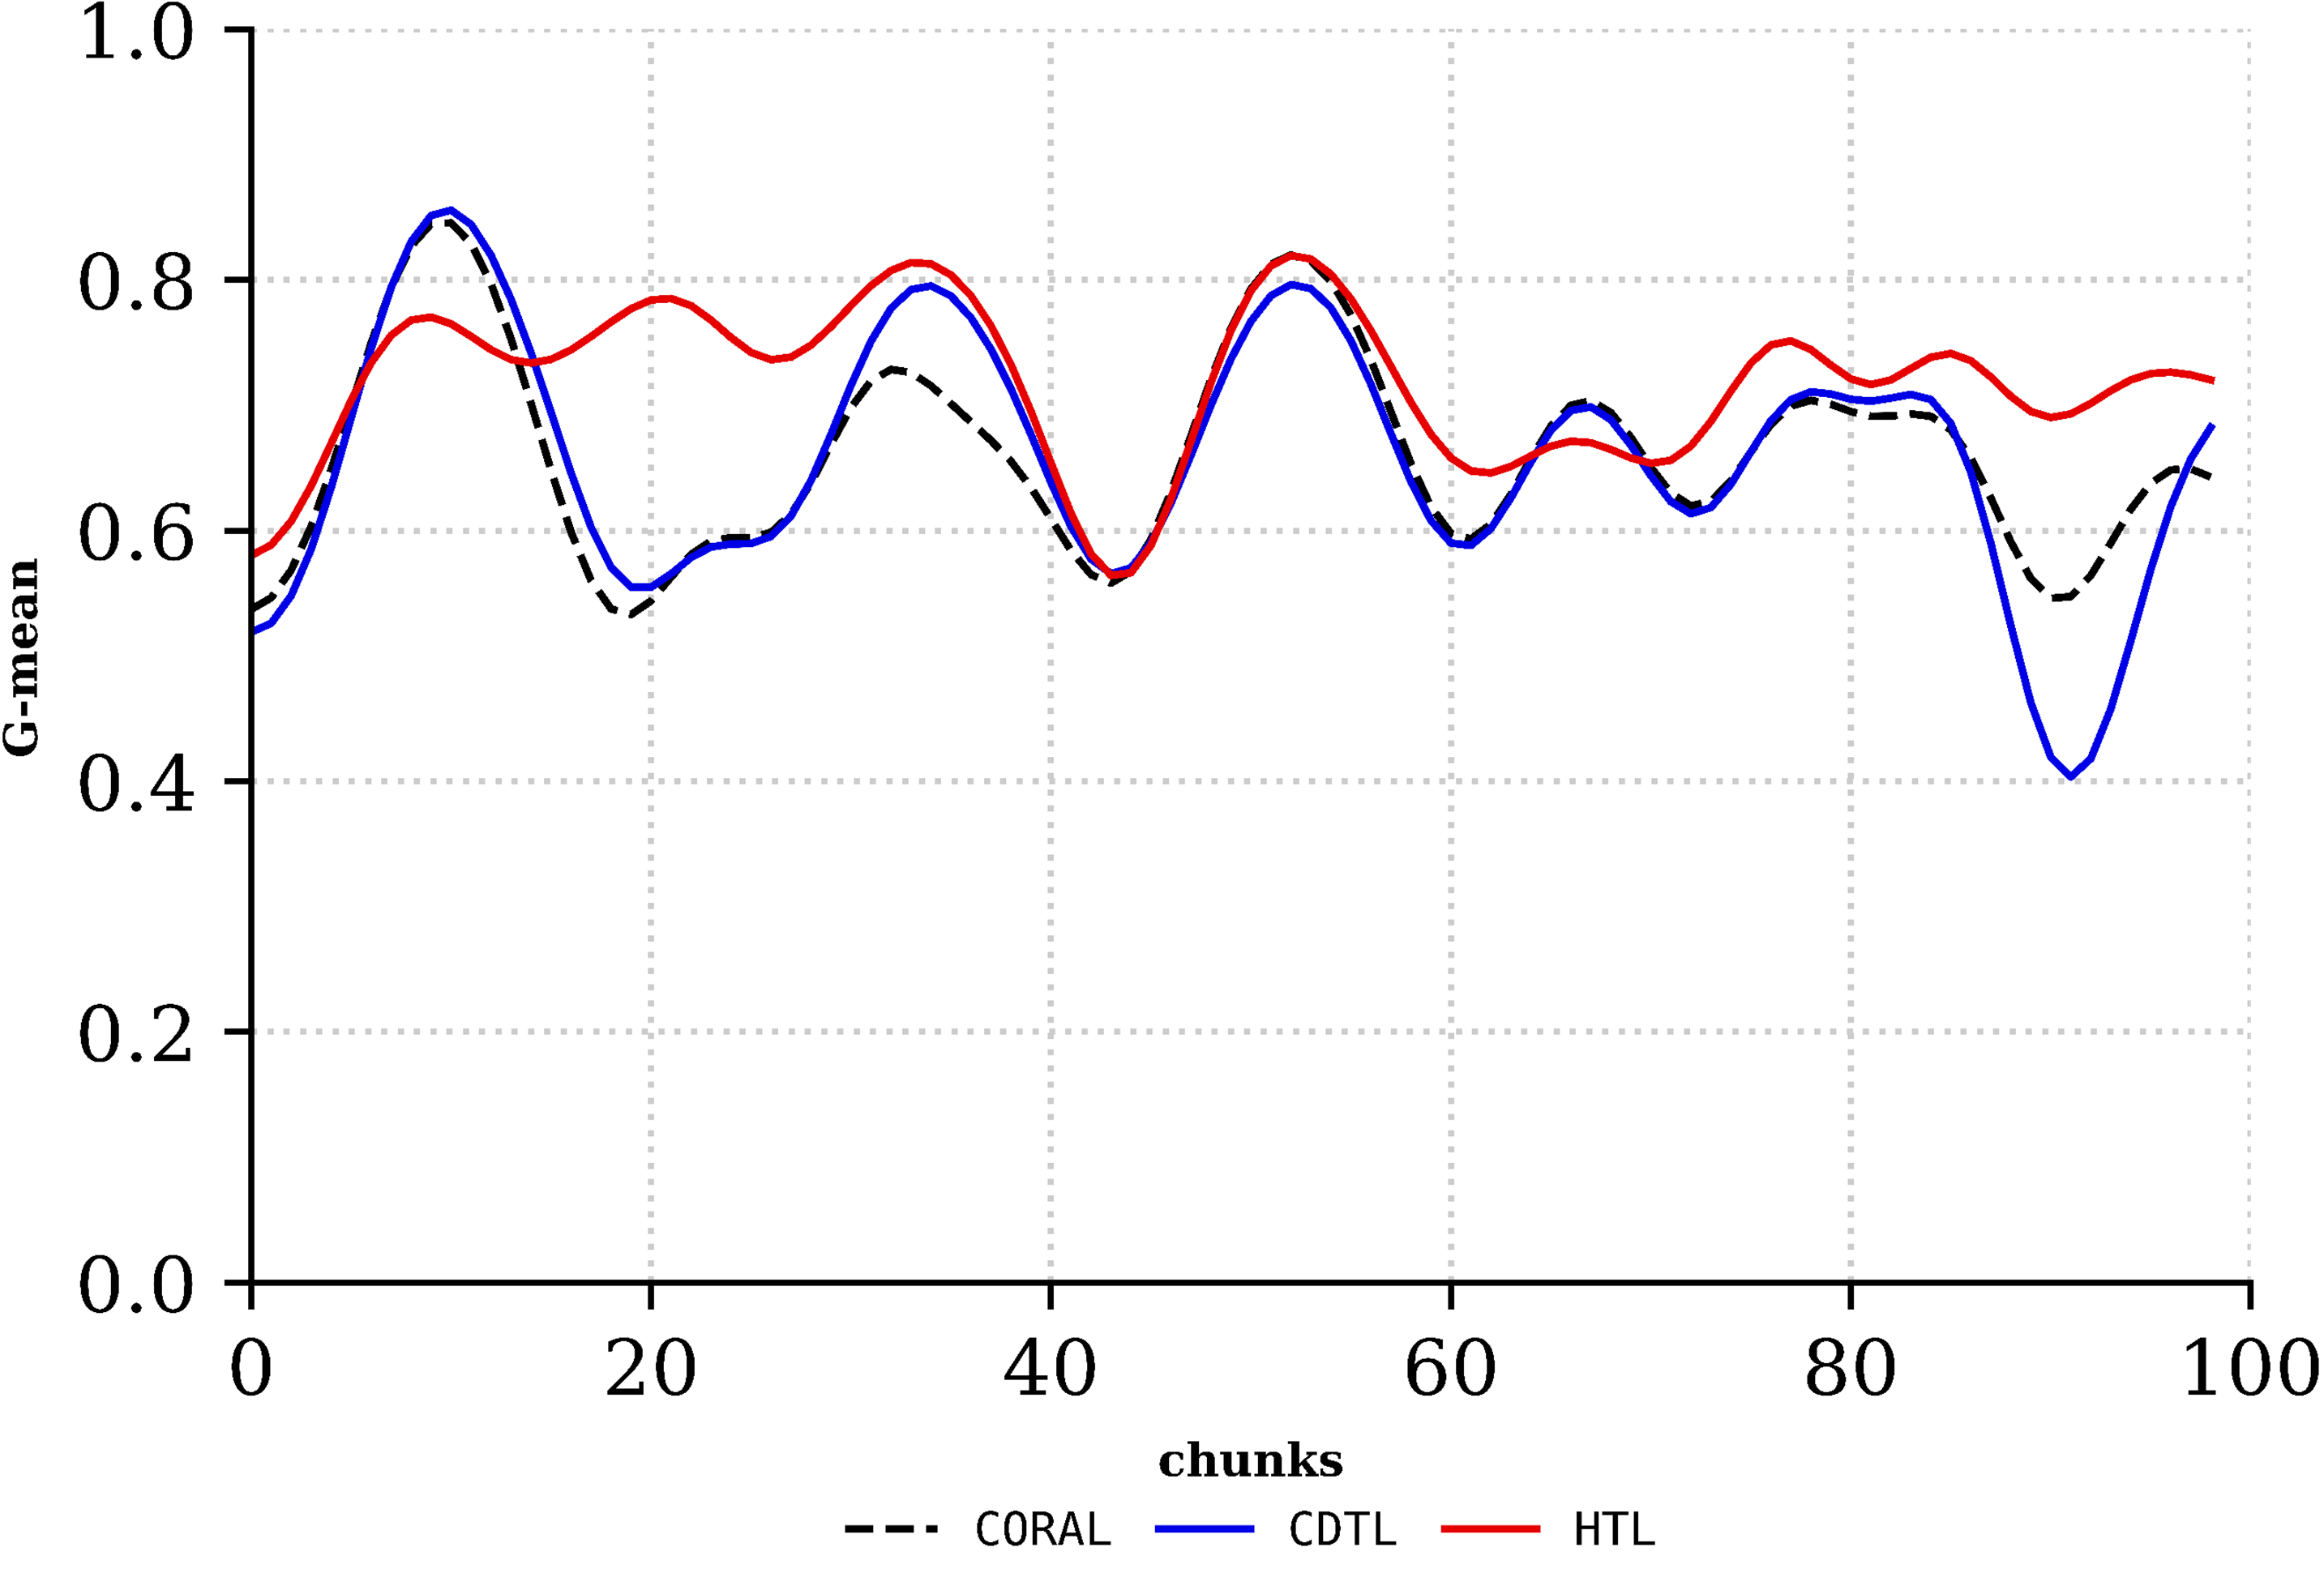
\includegraphics[width=0.6\linewidth]{6_transfer_learning/figures/exp2_1.png}
  \caption{Performance results of the Covertype Stream as the target domain with multiple heterogeneous source domains.}
	\label{fig:6_exp4}
\end{figure}
Figures \ref{fig:6_exp4} and \ref{fig:6_exp5} delve into the impact of incorporating multiple heterogeneous source domains on the classification performance of various methods, offering a nuanced philosophical reflection on the interplay between diversity, adaptability, and resilience in dynamic environments. In Figure \ref{fig:6_exp4}, the Covertype data stream serves as the target domain, while Synthetic-8, Synthetic-52, and Sensor streams act as heterogeneous source domains. The results demonstrate a notable improvement over previous experiments, underscoring the epistemic value of increasing the number of source domains. This enhancement reflects the philosophical principle of cumulative epistemic diversity: as the pool of source domains expands, the system gains access to a broader spectrum of positive knowledge. Each additional domain contributes incrementally to the refinement of classifiers, facilitating more accurate and adaptive performance.

Figure \ref{fig:6_exp5}, employing the same experimental setup but switching the target domain to the Sensor stream, highlights the influence of contextual factors on performance. The Sensor stream introduces higher noise levels and frequent concept drifts, presenting significant challenges to all methods. Despite these adversities, HTL consistently achieves superior performance across all chunks, reinforcing its adaptability and capacity to navigate complex and unstable environments. This robustness aligns with a philosophical framework that values resilience and context-sensitive adaptation in epistemic systems. In contrast, CORAL and CDTL exhibit nearly identical performance values across most chunks, indicating a more static approach to adaptation. Their inability to capitalize fully on the heterogeneity of source domains or mitigate the challenges posed by the Sensor stream underscores the philosophical tension between generality and specificity in dynamic learning systems. While they may perform adequately in stable or homogenous contexts, their relative rigidity limits their efficacy in environments marked by noise and drift.
\begin{figure}[H]
	\centering
	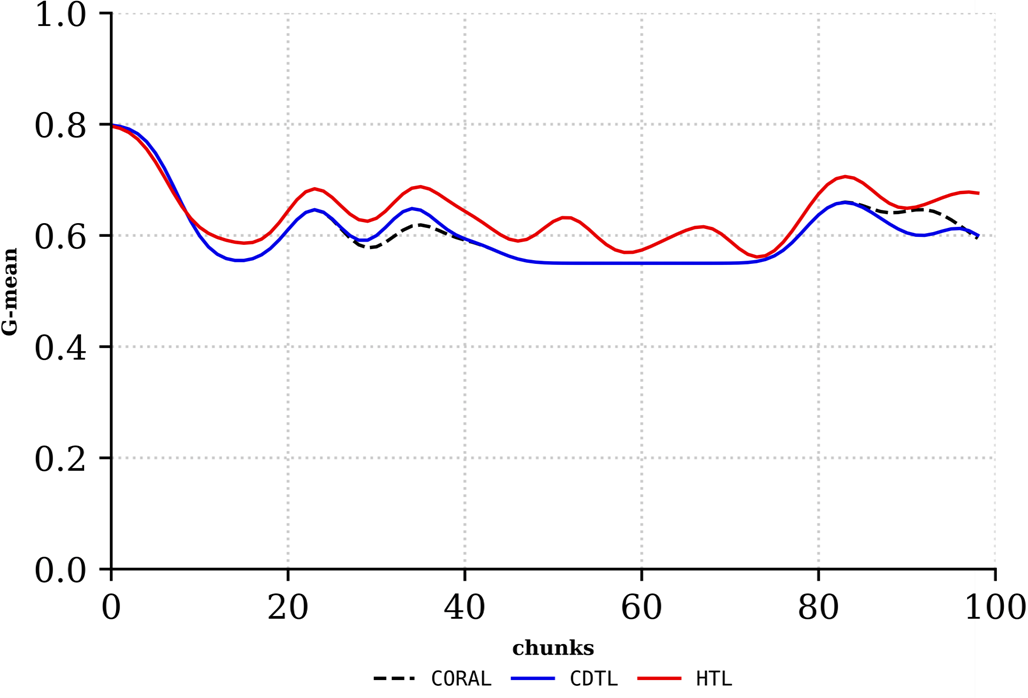
\includegraphics[width=0.6\linewidth]{6_transfer_learning/figures/exp3.png}
  \caption{Results of the Sensor Stream as the Target Domain with Multiple Heterogeneous Source Domains.}

	\label{fig:6_exp5}
\end{figure}

\subsubsection{Results on One Heterogeneous Source Domain}
This section evaluates the overall performances of CORAL, CDTL, and HTL across five performance metrics: $f_1$ score, precision, recall, G-mean, and BAG. Table \ref{table:6_table2} summarizes the average performance across 100 data chunks for each method and highlights HTL's consistent superiority in most configurations.

In the first experiment, which lacked a source domain, CORAL achieved the highest precision, while HTL excelled across the other metrics. In subsequent experiments, HTL consistently outperformed other methods in most metrics, except for recall in the third experiment, where CDTL achieved the best results. The performance improvement across experiments reflects the incremental addition of source domains, which enhances the positive knowledge available to the classifiers, thereby improving overall performance.
  
\begin{table}[H]
  \centering
  \caption{Comprehensive performance comparison of CORAL, CDTL, and HTL across all previous experiments.}
  \resizebox{\textwidth}{!}{
  \begin{tabular}{|l|l|c|c|c|}
  \hline
  \textbf{Experiment}                            & \textbf{Metric} & \textbf{CORAL} & \textbf{CDTL} & \textbf{HTL} \\ \hline
  \multirow{4}{*}{Without source domain}         & BAC             & 0.723          & 0.723         & \textbf{0.725} \\ \cline{2-5} 
                                                 & G-mean          & 0.652          & 0.654         & \textbf{0.717} \\ \cline{2-5} 
                                                 & $f_1$ score        & 0.875          & 0.874         & \textbf{0.890} \\ \cline{2-5} 
                                                 & Precision       & 0.827          & 0.823         & \textbf{0.851} \\ \cline{2-5} 
                                                 & Recall          & \textbf{0.950} & 0.944         & 0.939          \\ \hline
  \multirow{4}{*}{Homogenous source domain}      & BAC             & 0.731          & 0.730         & \textbf{0.755} \\ \cline{2-5} 
                                                 & G-mean          & 0.658          & 0.653         & \textbf{0.717} \\ \cline{2-5} 
                                                 & $f_1$ score        & 0.876          & 0.875         & \textbf{0.858} \\ \cline{2-5} 
                                                 & Precision       & 0.830          & 0.829         & \textbf{0.851} \\ \cline{2-5} 
                                                 & Recall          & 0.950          & 0.950         & \textbf{0.953} \\ \hline
  \multirow{4}{*}{Single heterogeneous source domain} & BAC         & 0.732          & 0.732         & \textbf{0.757} \\ \cline{2-5} 
                                                 & G-mean          & 0.661          & 0.657         & \textbf{0.717} \\ \cline{2-5} 
                                                 & $f_1$ score        & 0.875          & 0.875         & \textbf{0.859} \\ \cline{2-5} 
                                                 & Precision       & 0.835          & 0.835         & \textbf{0.851} \\ \cline{2-5} 
                                                 & Recall          & 0.947          & 0.950         & \textbf{0.953} \\ \hline
  \multirow{4}{*}{Multisource heterogeneous domain (Covertype stream)} & BAC & 0.732  & 0.732         & \textbf{0.757} \\ \cline{2-5} 
                                                 & G-mean          & 0.661          & 0.661         & \textbf{0.717} \\ \cline{2-5} 
                                                 & $f_1$ score        & 0.875          & 0.875         & \textbf{0.859} \\ \cline{2-5} 
                                                 & Precision       & 0.835          & 0.835         & \textbf{0.851} \\ \cline{2-5} 
                                                 & Recall          & 0.947          & 0.950         & \textbf{0.953} \\ \hline
  \multirow{4}{*}{Multisource heterogeneous domain (Sensor stream)} & BAC & 0.998  & 0.998         & \textbf{0.998} \\ \cline{2-5} 
                                                 & G-mean          & 0.971          & 0.971         & \textbf{0.992} \\ \cline{2-5} 
                                                 & $f_1$ score        & 0.997          & 0.997         & \textbf{0.997} \\ \cline{2-5} 
                                                 & Precision       & 0.998          & 0.998         & \textbf{0.998} \\ \cline{2-5} 
                                                 & Recall          & 0.998          & 0.998         & \textbf{0.998} \\ \hline
  \end{tabular}
  }

  \label{table:6_table2}
  \end{table}

\subsection{Analysis Runtime between CORAL, CDTL, and HTL Techniques}
From a philosophical perspective, the experimental results underscore the nuanced interplay between technological efficiency and contextual suitability in heterogeneous transfer learning. The choice of an optimal algorithm emerges not as an absolute truth but as a contextual decision shaped by the characteristics of the dataset and the temporal demands of the application. The study’s findings illuminate the inherent efficiency of the HTL algorithm, particularly in scenarios demanding rapid iteration. For instance, the HTL algorithm's completion of 100 iterations within 304 seconds in the homogeneous source domain setting starkly contrasts with the prolonged runtimes of CORAL and CDTL algorithms. This efficiency is not merely a quantitative advantage but symbolizes the evolving imperative of time-conscious adaptability in machine learning \cite{ref}. The philosophical significance deepens when considering the diverse source domain configurations—homogeneous, absent, single heterogeneous, and multi-source heterogeneous—each representing varying degrees of complexity and unpredictability. The HTL algorithm's consistent efficiency across these scenarios reflects a harmonious balance between universality and specificity. It challenges the idea of algorithmic rigidity, suggesting that adaptability and context-awareness are the cornerstones of effective machine learning paradigms \cite{ref}. Thus, the findings, accentuated by the runtime data in Table \ref{table:6_table3}, reveal the HTL algorithm as not merely a technical tool but a conceptual embodiment of efficiency tailored to the exigencies of dynamic, real-world applications. In this light, its superiority is not only functional but philosophical, aligning with the broader pursuit of practical excellence in algorithmic design and implementation.
\begin{table}[H]
  \centering
  \caption{Runtimes (in seconds) for CORAL, CDTL, and HTL.}
  \resizebox{\textwidth}{!}{
  \begin{tabular}{|l|l|l|c|c|c|}
  \hline
  \textbf{Experience}                              & \textbf{Target domain} & \textbf{Source Domain}                      & \textbf{CORAL} & \textbf{CDTL} & \textbf{HTL} \\ \hline
  without source domain                            & Covertype              & None                                         & 312            & 312           & \textbf{304} \\ \hline
  Homogenous source domain                         & Covertype              & Synthetic-52                                 & 6165           & 614           & \textbf{606} \\ \hline
  Single heterogeneous source domain               & Covertype              & Synthetic-8                                  & 6060           & 4703          & \textbf{4475} \\ \hline
  Multi-source heterogeneous domain                & Covertype              & Sensor, Synthetic-52, and Synthetic-8        & 23011          & 14043         & \textbf{13824} \\ \hline
  Multi-source heterogeneous domain                & Sensor                 & Covertype, Synthetic-52, and Synthetic-8     & 14524          & 3052          & \textbf{3005} \\ \hline
  \end{tabular}
  }
  \label{table:6_table3}
  \end{table}
  
\subsection{Analysis performance and runtime of HTL for online learning and chunk-based concept drift}

This experiment explores the temporal dynamics of various learning techniques, comparing the efficiency of online learning with chunk-based concept drift methods. The time savings provided by drift detectors like EDDM and ADWIN offer insights into the relationship between learning time and performance. The EDDM drift detector is notably efficient, detecting 40 drifted chunks out of 100, which highlights a pragmatic approach to reducing computational overhead while maintaining accuracy. This efficiency aligns with the concept of "pragmatic optimization," aiming to balance time and performance within real-world constraints \cite{ref}. In contrast, the ADWIN drift detector, which detects 63 drifted chunks and requires 63 learning times, demonstrates a trade-off between improved drift detection and time efficiency. This suggests that optimal performance is often context-dependent, with the most efficient algorithm not necessarily being the one that minimizes time, but one that balances all relevant factors. On the other hand, online learning, requiring 100 learning times for 100 chunks, proves to be the least time-efficient. However, its design may reflect a commitment to consistency and robustness, even at the expense of time.
Figures \ref{fig:6_exp6} and \ref{fig:6_exp7}, which include radar and line diagrams, visually capture the tension between time efficiency and performance. While online learning achieves optimal performance, its higher time consumption highlights the conflict between pursuing perfection and managing resource limitations. This analysis emphasizes that efficiency is not solely about minimizing time but involves balancing multiple factors in real-world applications.
\begin{figure}[H]
	\centering
	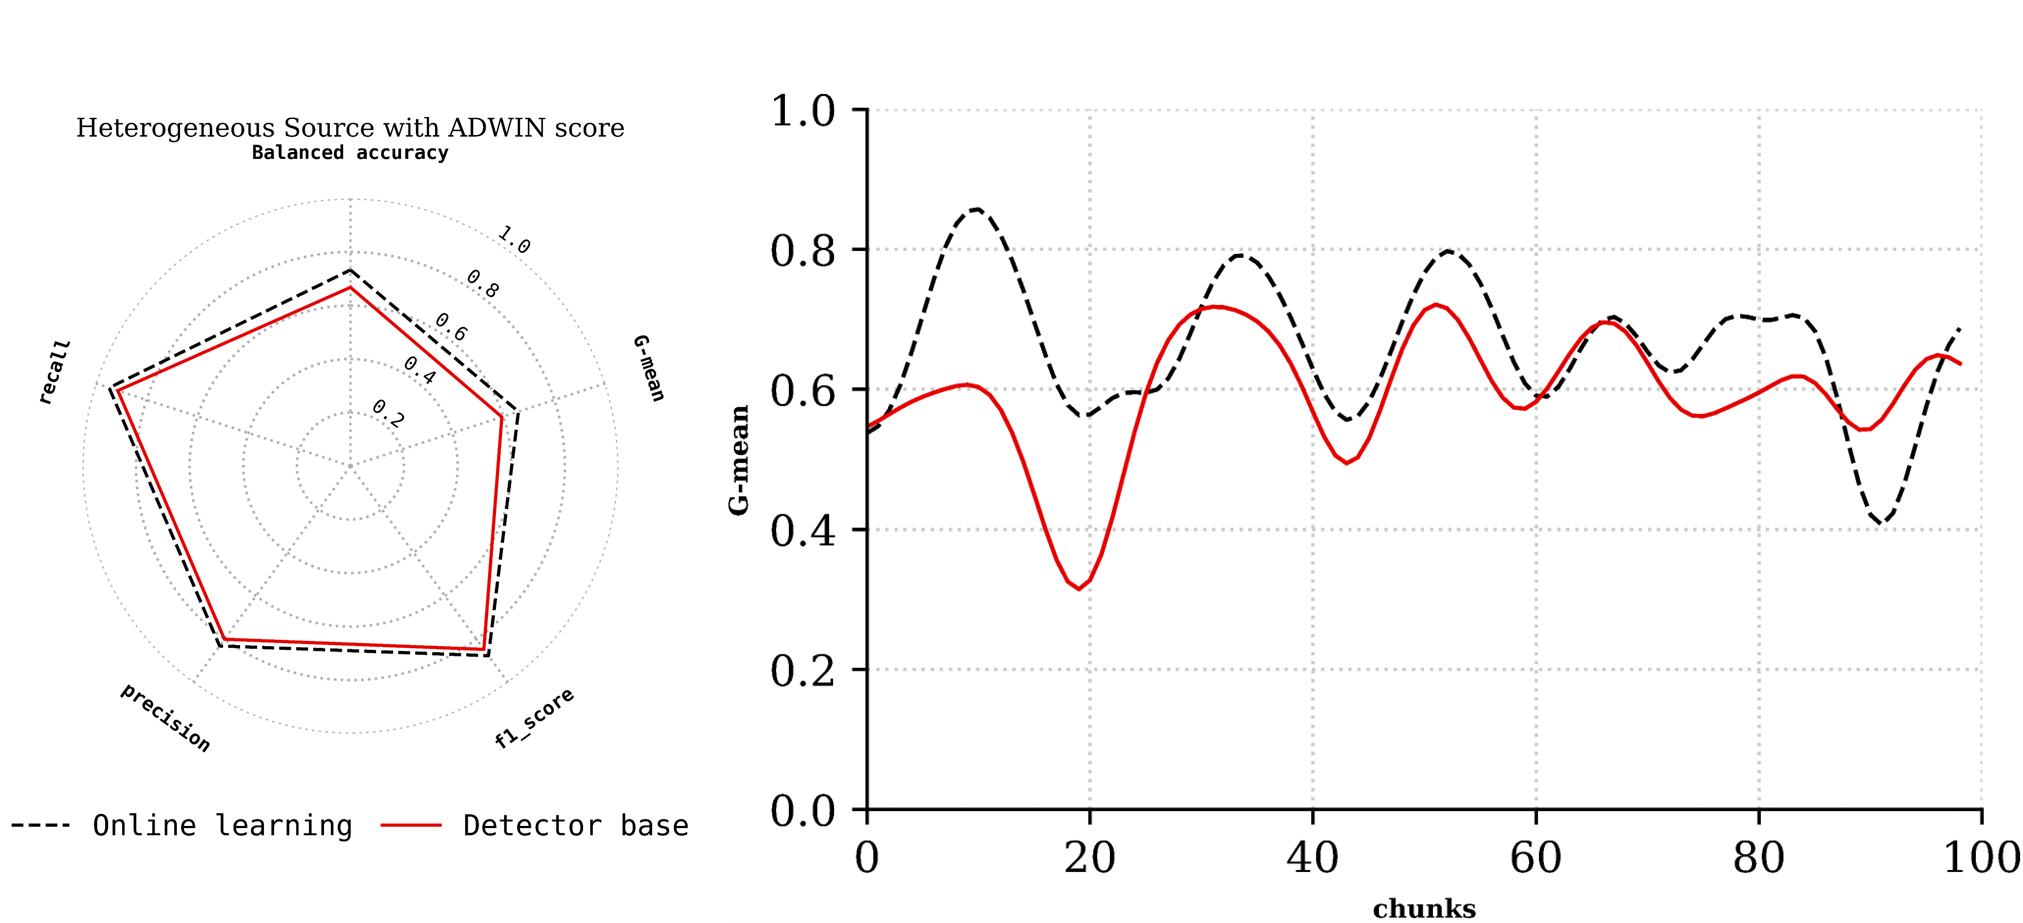
\includegraphics[width=1\linewidth]{6_transfer_learning/figures/exp4.png}
	\caption{Online learning and chunk-based results for the Covertype stream using the ADWIN detector.}
	\label{fig:6_exp6}
\end{figure}

\begin{figure}[H]
	\centering
	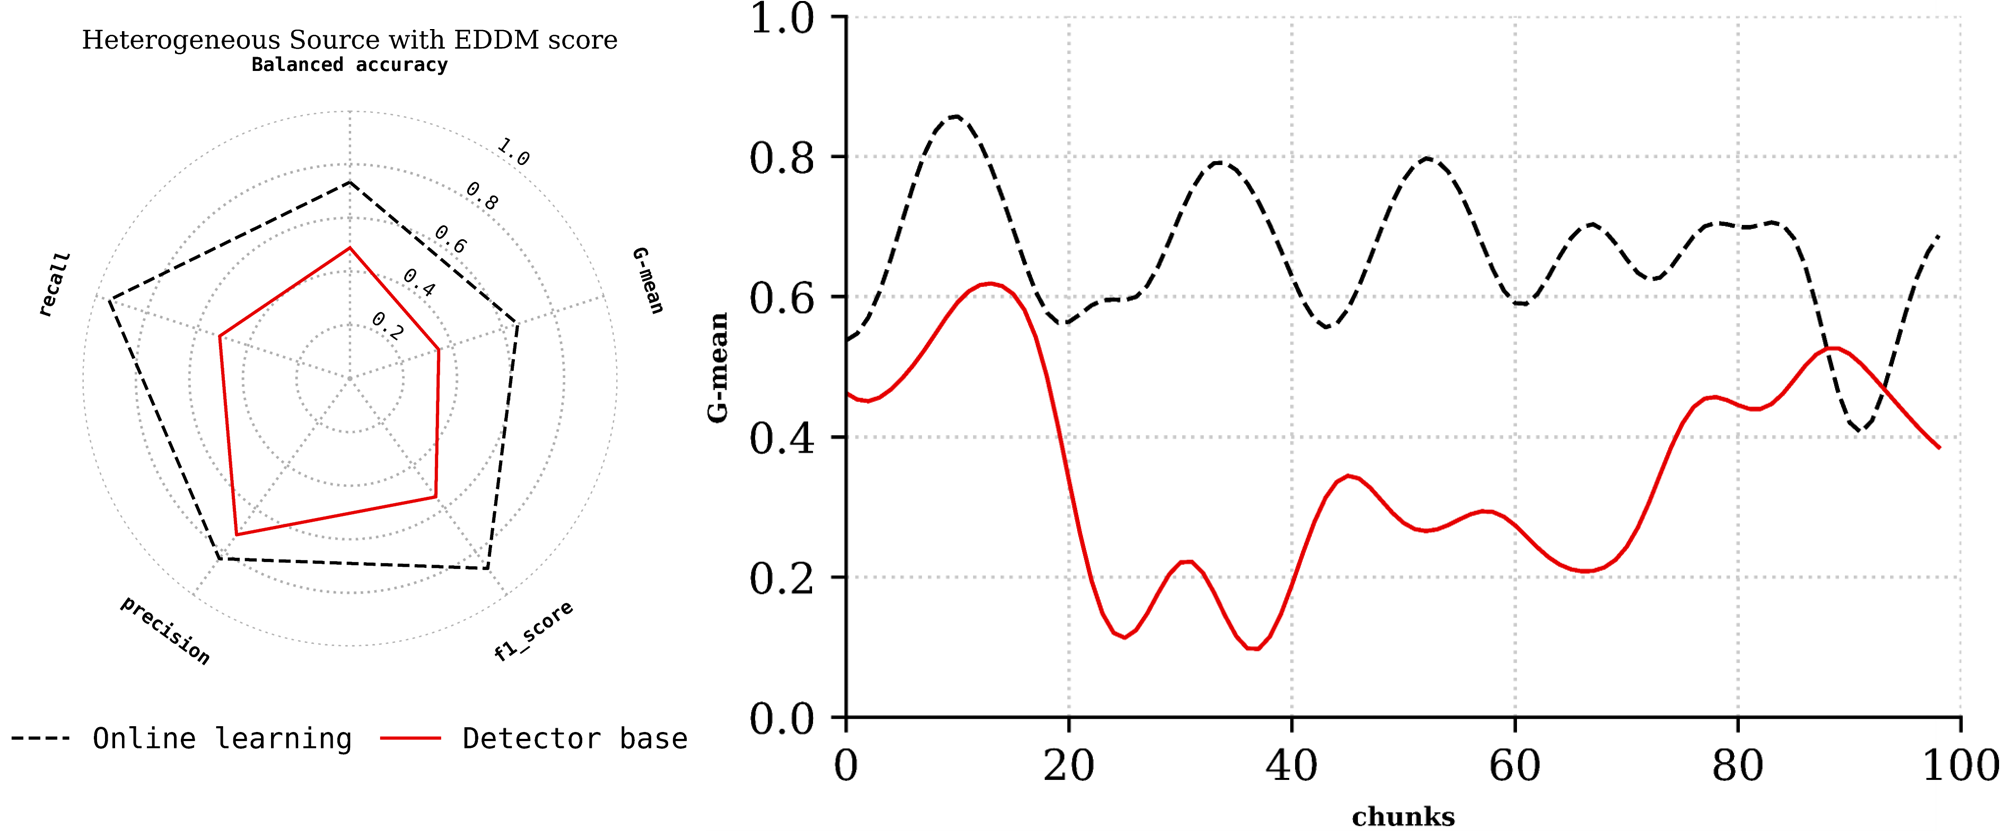
\includegraphics[width=1\linewidth]{6_transfer_learning/figures/exp5.png}
  \caption{Results of online learning and chunk-based detection in the Covertype stream using the ADWIN detector.}
	\label{fig:6_exp7}
\end{figure}
The comparison between online learning, the EDDM detector, and ADWIN reflects a broader philosophical consideration of efficiency, adaptability, and the balance between idealism and practicality. Online learning, with its ability to achieve optimal performance, represents an ideal approach—constantly evolving, adapting to real-time data without reliance on prior knowledge. This continuous adaptation mirrors the notion of becoming, where the system remains in a state of perpetual growth and refinement. The radar diagrams in Figure \ref{fig:6_exp7} further emphasize the superiority of online learning, positioning it as the most effective method. ADWIN, in this context, stands as a favorable compromise, balancing the strengths of online learning with the practicality of reduced time expenditure. ADWIN thus exemplifies the concept of harmony, where competing forces of performance and efficiency are reconciled, offering an adaptable solution that doesn’t strive for perfection but achieves a satisfactory balance. In contrast, the EDDM detector, with its lower performance, reflects the limitations of rigidity—remaining static in the face of evolving data, it fails to respond effectively to dynamic changes. This serves as a reminder of the consequences of inflexibility in systems, where an inability to adapt leads to diminished overall effectiveness. Ultimately, in environments characterized by chunk-based concept drift, especially with the ADWIN detector, the approach that ensures high performance while minimizing computational costs reveals itself as ideal. This balance speaks to the philosophical principle of achieving optimal results through continuous yet measured adaptation \cite{gama2004learning, madkour2023historical}.

\begin{table}[H]
  \centering
  \caption{Runtimes (in seconds) for the Online Learning, ADWIN, and EDMM.}
  \begin{tabular}{|l|c|c|}
  \hline
  \textbf{Technique}       & \textbf{Runtime (in seconds)} & \textbf{Learning Times} \\ \hline
  Online Learning          & 3102             & 100                     \\ \hline
  ADWIN detector           & 2257             & 63                      \\ \hline
  EDMM detector            & 1948             & 40                      \\ \hline
  \end{tabular}
  \label{table:6_table4}
  \end{table}


% automl_evaluation
% % this file is called up by thesis.tex
% content in this file will be fed into the main document

% this file is called up by thesis.tex
% content in this file will be fed into the main document

%: ----------------------- introduction file header -----------------------


\begin{savequote}[50mm]
It is strange that only extraordinary men make the discoveries, which later appear so easy and simple.
\qauthor{Georg C. Lichtenberg}
% The beginning is the most important part of the work.
% \qauthor{Plato}
\end{savequote}


\chapter{A Guided Search for MCS pruning}
\label{ch5_GUided_MCS_Pruning}

In chapter \ref{chapter4_training-set}, two intelligent paradigms have been discussed to enhance the performance of MCS. First, \textit{on data level} via applying IS techniques to learn from representative samples. Second, \textit{on the fusion level} via applying SI algorithms to combine a set of classifiers. However, the complexity of the investigated MCS is proportional to both the number of classes and the number of individual models. For example, to solve a 10-class problem using 200 classifiers, each candidate from the population of SI will be composed of 2000 elements (matrix of 10 $\times$ 200). This chapter discusses the alternative procedure to tackle this challenge. First, to keep on applying the IS techniques in the first part. Second. to perform a guided search for pruning the generated MCS. 

Building ensemble models, in general, requires an answer to the following questions \cite{xu1992} (1) How many classifiers should we use? (2) What type of classifiers should be chosen? (3) Which feature subset should be presented to each classifier? (4) Which combination rules to be used?. To answer the above questions, the authors in \cite{kuncheva2003,dietterich2000}  argued that ensemble members should have both high accuracy and high diversity to gain more. Hence, manipulation of algorithms \cite{sesmero2015} and manipulation of the features \cite{rodriguez2006}  are answers to 2nd and 3rd questions, to obtain different model structures that are trained from diverse feature spaces. Regarding the combination methods; many strategies, which vary between trained \cite{sesmero2015,wozniak2010} or untrained \cite{krawczyk2016,kuncheva2014}, have been applied and also been analyzed in  \cite{kuncheva2014a}. In this chapter, we concentrate on answering the 1st question via overproducing many learning models followed by ensemble pruning. The general objective is to improve the overall accuracy, speed up the classification process, and to save the computational and storage resources.


Despite the remarkable performance of the ensemble methods, a large-size ensemble can be considered as a drawback. In \cite{margineantu1997} and related to the investigated classification tasks, it has been noticed that the ensemble size can be reduced up to 60-80\% without significant deterioration to its performance. Therefore, it is practically useless to keep all the ensemble members for the prediction process. In addition, when the models are distributed over a network, the reduction of models leads to the reduction of communication costs \cite{tsoumakas2009}. A possible solution to downsize/prune MCS can be broadly divided into the following five solutions \cite{onan2017,mendes2012}:
 

 \begin{itemize}[noitemsep]
     \item \textbf{Exhaustive search:} Requires an evaluation to all the possible $2^{T}-1$ nonempty subsets of classifiers. However, this is an NP-combinatorial search problem as the complexity grows exponentially with the ensemble size. Exhaustive search methods are only applicable when the number of classifiers is small \cite{sharkey2000}, while they are unfeasible for typical large-size ensembles \cite{martinez2009}.
     \item \textbf{Optimization-based search:} Meta-heuristic search methods are the alternative to offer huge computational savings. All the search methods in this category optimize an evaluation metric. The metric can be diversity \cite{shipp2002} in an attempt not to select similar classifiers and to obtain complementary subsets. Another popular metric is to reduce the ensemble error of a particular combination rule. Genetic Algorithms have been shown to find near-optimal solutions \cite{adnan2016}. Other evolutionary-based search methods showed comparable performance with faster convergence rate such as: Tabu search \cite{roli2002} and population-based incremental learning \cite{ruta2001b}. In general, the computational costs of these techniques are still rather large.
     \item \textbf{Sequential search:} The following strategies can be applied to find the preferred ensemble subset;
     \begin{enumerate}[nosep]
         \item [-] \textit{Forward Search}: Starts with an empty set followed by sequential addition, one classifier at a time, and conditioned by enhancing specific metrics; otherwise, the search stops. There is no guarantee to find the optimal subensemble.
         \item[-] \textit{Backward Search}: The algorithm starts with the whole ensemble size, and one classifier is removed iteratively without affecting the evaluation metric. The complexity of this algorithm is the same as in forward search. 
     \end{enumerate}

    \item \textbf{Clustering-based pruning:} Clustering techniques, non-supervised methods, are used to group similar classifiers together. The formed clusters are separately pruned to select a high diversity classifiers' subset. This methodology could suffer from cluster instability as mentioned in \cite{lin2014}, whereas an alternative solution is in using hybrid clustering techniques, consensus clustering, to aggregate different clustering results \cite{onan2017,ghosh2011}.    
       \item \textbf{Ranking-based pruning} (Ordering-based pruning): Firstly, the classifiers are ranked based on an evaluation criteria, then the top set in the list is selected. The computational costs of these methods are less in comparison with the aforementioned solutions. In addition, these methods are more efficient to work with parallel ensembles where individual classifiers can be built independently.
 \end{itemize}
 
 
 In this chapter, a guided search-based pruning method is proposed to consider both the individual's accuracy and the ensemble diversity to improve the overall accuracy, in the light of reduced data in advance. The remainder of this chapter is organized as follows: In Section \ref{ch5_motivations},
the motivations and the contributions are presented. While in Section \ref{ch5_ordering_pruning}, the concept of ensemble pruning via reordering the classifiers is explained. The proposed framework is to be presented in detail in Section \ref{ch5_methodology}. The experimental results are presented in Sections \ref{ch5_expsetup}. Finally, Section \ref{ch5_conclusions}  will be dedicated for the conclusions and future work.



\section{Motivations and Contributions} \label{ch5_motivations}
The main contributions of this chapter can be highlighted in the following points:

\begin{enumerate}[nosep]
    \item  Forming small-size ensembles with less complex individual models.
    \item  Proposing a guided search-based ensemble pruning method.
     \item Analyzing how the proposed method can be an alternative to large-size ensembles.
    
    \item Getting out more accuracy from the reduced data and comparing it with state-of-art ensembles (Random Forest \cite{breiman2001}, SAMME \citep{hastie2009}, and XGBoost \citep{chen2016}) that are trained from nonreduced data. 
\end{enumerate}

\section{Ordering-based Pruning} \label{ch5_ordering_pruning}

As mentioned before, those strategies are more promising to select an efficient subensemble in less computational time. In bagging, the base classifiers are generated independently based on different bootstrap samples from the training data. The prediction accuracy of the ensemble is positively correlated with the number of aggregated models. Notwithstanding, the accuracy of the ensemble levels off after some point. After this point the inclusion of further models becomes useless. As shown in \cite{martinez2004,martinez2009}, the general accuracy (error) can be maximized (minimized) by changing the order in which the classifiers are aggregated. The authors proved that the first 20\% from the modified ordered bagging ensemble was sufficient to speed up the classification decision, to save memory storage, and to get an improved composite prediction. The core component in the ordering strategies is the heuristic metric used to give the ordering process. That metric exploits the aggregation relationship between the classifiers based on maximizing (minimizing) specific measure as in greedy search \cite{cao2018,martinez2004,margineantu1997} or rank the significance of each base classifier in one batch as in \cite{guo2013,guo2018,lu2010}. These ordering metrics require a selection or pruning set composed of labeled samples, $D_{pr}$, to validate and guide the ordering process. For that, the pruning set can be an independent part, not used for training, or can be sampled from the original training. After that, the predictions of the selected classifiers are aggregated by unweighted voting as: 

\begin{equation}
\label{consensus}
\hat{\Psi}(\textbf{x}_i)=\mathop{\arg\max}\limits_{y_i \in {M}} \mathop{\sum}\limits_{k=1}^{\hat{T}} \left[\Psi_{k}(\textbf{x}_i)=y_i\right] \; 
\end{equation}
%in Eq. (\ref{consensus}), 
where $[\;]$ denotes Iverson's bracket and $\hat{T}$ represents the subensemble size. As a promising strategies, we concentrate on common ordering-based pruning methods from the literature review with the discovered challenges. 




\subsection{Diversity Contribution of Individuals} \label{ch5_EPIC.div}
Ensemble Pruning via Individual Contributions (EPIC) is introduced in \cite{lu2010}. The appropriate handling of the trade-off between diversity and the accuracy of the ensemble members is the key to gain efficient ensemble models \cite{kuncheva2003,zhang2006,barak2017}. Increasing the accuracy of individual models leads to producing similar classifiers, in their decisions, with less integration in-between \cite{lu2010} due to lack of diversity. Two research assumptions have been mentioned in \cite{lu2010} with deep analysis of the first one: (1) When two ensembles have individual models with the same accuracy, the more diverse ensemble should perform better. (2) When two ensembles are similarly diverse, the one which has more accurate individuals should perform better. These two assumptions represent the balance between ensemble diversity and the individual's accuracy, respectively. The classifier’s rank shouldn’t be assigned  based on its accuracy alone, but further on how it is more diverse with the majority voting of the ensemble (\textit{different from peer members}).

During the simple majority voting over a specific sample $\textbf{x}_i$, the classifier's prediction can be categorized into one of four cases (a) Correct Prediction, but ensemble prediction is incorrect (b) Correct Prediction and ensemble prediction is also correct (c) Incorrect Prediction, but ensemble prediction is correct (d) Incorrect Prediction and ensemble prediction is incorrect. The classifiers belong to case (a) are more critical to change the ensemble decision by giving them higher priority to be selected, hence reducing the effect of negative voting. While classifiers in the category (c) receive a lower rank, even their presence in the ensemble is less harmful.


EPIC \cite{lu2010} measures the diversity contribution of each individual  via Equation (\ref{ch5_EPIC}), where $\nu_{max}^{(i)},\nu^{(i)}_{sec}$ are the number of votes for the top two classes over sample $\textbf{x}_i$ respectively. While $\nu_{\Psi_{k}(\textbf{x}_i)}^{(i)}$ denotes the number of classifiers that agree with the prediction $\Psi_{k}(\textbf{x}_i)$ (including itself), and $\nu_{correct}^{(i)}$ denotes number of votes of the correct prediction over sample $\textbf{x}_i$. 


\begin{equation}
\label{ch5_EPIC}
\scalemath{0.92}{
    \begin{aligned}
     IC_{k}=\mathop{\sum}\limits_{i=1}^{N} \Bigg(\alpha_{ki}\ (2\nu_{max}^{(i)}-\nu_{\Psi_{k}(\textbf{x}_i)}^{(i)})   + \beta_{ki}\ \nu^{(i)}_{sec}
      + \theta_{ki}\ (\nu_{correct}^{(i)}-\nu_{\Psi_{k}(\textbf{x}_i)}^{(i)}-\nu_{max}^{(i)})  \Bigg) \\
      \end{aligned}
      }
      \end{equation}
      \textit{Where:} 
    \begin{align*}
      \alpha_{ki}&= \begin{cases} 
      1 & \text{if} \ \Psi_{k}(\textbf{x}_i)=y_i \ \land \Psi_{k}(\textbf{x}_i)\ \text{is in the minority voting\ssep}\\
      0 & \text{otherwise}. 
   \end{cases}   \\
   \beta_{ki}&=\begin{cases} 
      1 & \text{if} \ \Psi_{k}(\textbf{x}_i)=y_i \ \land \Psi_{k}(\textbf{x}_i)\ \text{is in the majority voting\ssep}\\
      0 & \text{otherwise}. 
   \end{cases}   \\ 
    \theta_{ki}&=\begin{cases} 
      1 & \text{if} \ \Psi_{k}(\textbf{x}_i)\neq y_i \ssep\\
      0 & \text{otherwise}. 
   \end{cases}\\
   \end{align*}
   
In \cite{lu2010}, the authors concluded that classifiers that have more votes in the minority groups bring more diversity contributions to the ensemble and contain more useful knowledge for constructing subensembles. Those classifiers are assigned a higher positive degree of contribution for their correct prediction and less negative degree of contribution for their incorrect prediction.      
   
   
   

\subsection{Unsupervised Ensemble Margin}
\label{ch5_UMEP}
Unsupervised Margin based Ensemble Pruning (UMEP) has been proposed in \cite{guo2013} with the focus on classifier properties to  classify the hard patterns correctly. The innovation of this metric is based on measuring the margin of $\textbf{x}_i$. The larger the margin of $\textbf{x}_i$ the more certain its classification is. As in boosting \cite{freund1997}, the idea of this method is to focus on low margin instances. The absolute margin of $\textbf{x}_i$ can be measured from ensemble decisions as:
 \begin{equation}
\label{margin.x}
\text{Margin}(\textbf{x}_i)=(\nu_{max}-\nu_{sec}) \bigg/{\mathop{\sum}\limits_{i=1}^M (\nu_{c_i})} 
\end{equation}


This measure considers only the difference between the votes of the top two classes $(\nu_{max},\nu_{sec})$ over the sample $\textbf{x}_i$. For that, it is an unsupervised measure that does not require the true class label. Here the margin takes a value in the interval $[0,1]$. The set of samples, $\textbf{x}_i$ $\in D_{pr}$, that are classified correctly by each classifier will be considered for calculating it's margin-based information quantity as:
\begin{equation}
\label{psi.margin}
\Psi_k(D_{pr})=\frac{-1}{N}{\mathop{\sum}\limits_{i=1}^N    \log{}(\text{Margin}(\textbf{x}_i)) \quad \Big|  \Psi_k(\textbf{x}_i)=y_i } 
\end{equation}
Then, the classifiers are ranked based on descending the measured values from Equation (\ref{psi.margin}). The more hard samples which are predicted correctly by the classifier, the more rank it receives to be included in the subensemble.

\subsection{Margin \& Diversity} \label{ch5_MDEP}
Margin and Diversity-based Ensemble Pruning (MDEP) \cite{guo2018} considers two aspects to better reorder the set of classifiers: (1) focusing on examples with small absolute margin and (2) focusing on classifiers with large diversity contribution to the ensemble. The MDEP measures the rank of each classifier via Equation (\ref{MDEP}) $\forall \textbf{x}_i \in D_{pr}\big| \Psi_{k}(\textbf{x}_i)=y_i$. 

 \begin{equation}
\label{MDEP}
\text{MDEP}(\Psi_{k})= \sum_{\textbf{x}_i \in D_{pr}}^{}\Bigg[\alpha f_m(\textbf{x}_i)+ (1-\alpha) f_d(\Psi_{k},\textbf{x}_i)
\Bigg]  
\end{equation}


Where $\alpha \in [0,1]$ represents the balance of importance between the margin of examples and the ensemble diversity. $f_m(\textbf{x}_i)$ and $f_d(\Psi_{k},\textbf{x}_i)$ are the $\log{}$ functions of $\textbf{x}_i$'s margin and $\Psi_{k}$'s diversity contribution on $\textbf{x}_i$, are calculated via Equation (\ref{MDEP.margin}) and Equation (\ref{MDEP.diversity}), respectively. Where $\Bar{y_i} \neq y_i$ is the class that receives the maximum number of votes on $\textbf{x}_i$. The challenge of the MDEP metric is the dependence on the predefined value of $\alpha$ that controls the trade-off between focusing on classifiers that correctly predict hard samples or focusing on classifiers that increase ensemble's diversity.    




 \begin{equation}
\label{MDEP.margin}
f_m(\textbf{x}_i)= \log{}\Bigg(\Biggl| {\frac{\nu_{y_i}^{(i)}-\nu_{\bar{y}_i}^{(i)}}{{M}}} \Biggl|   \Bigg)
\end{equation}   
 
 \begin{equation}
\label{MDEP.diversity}
f_d(\Psi_{k},\textbf{x}_i)=  \log{}\Bigg( \frac{\nu_{y_i}^{(i)}}{M}    \Bigg)
\end{equation}      
 


Determining the value of $\alpha$ is not a trivial task and should be analyzed for each dataset separately. It can be tuned by searching for the best value in the range [0,1] through the cross-validation process, which is a time-consuming procedure.  Increasing the value of $\alpha$ directs the search process to select a subensemble that better classifies low margin samples. While reducing the value of $\alpha$ enforces the search process to select a subensemble with high diversity. We praise with the effect of $\alpha$ that has been discussed in \cite{guo2018}, in an attempt to capture this conflict, but restricted with parameter tuning.  





Our contribution related to this part is to propose a guided search pruning method that handles the bias in the subensemble search strategy. We prove how our proposed method is stable with different datasets without assuming any parameters in advance. Furthermore, this chapter discusses the importance of the instance selection method to form simpler ensembles. Moreover, in the literature review; the performance of the pruned ensemble often compared with the unpruned one. Here we extend this level of comparisons to include several baseline and efficient ensemble models as: Random Forest \cite{breiman2001}, SAMME \citep{hastie2009}, and XGBoost \citep{chen2016}. The next section discusses the proposed method to introduce a dual reduction to the formed ensemble.  





















%%%%%%%%%%%%%%%%%%%%%%%%%%%%%%%%%%%%%%%%%%%%%%%
%
%   Methodology
%
%%%%%%%%%%%%%%%%%%%%%%%%%%%%%%%%%%%%%%%%%%%%%%%
\section{Proposed Framework}
\label{ch5_methodology}

The proposed framework is graphically presented in Figure \ref{topology}. The training fold is reduced by AllKNN \cite{tomek1976} as an instance selection method to select representative samples. The selected data by AllKNN will be the source to build a group of heterogeneous classifiers. A pruning set is formed using stratified sampling with 70\% from the train. The pruning set will be the source to rank the individual classifiers during ensemble selection. Using this methodology, the following state-of-art ensembles will be trained for comparison purposes:

\begin{itemize}[nosep]
   \item[-] RFSM: Random Forest \cite{breiman2001} is learned from the selected data.
   \item[-] UNP: The proposed heterogeneous classifiers, Section (\ref{proposed.mcs}), without pruning  learned from the selected data.
   \item[-] RFCOM: Random Forest is learned from the whole training data.
   \item[-] SAMME: (Stagewise Additive Modeling
using a Multi-class Exponential loss function \cite{hastie2009}), which is trained from whole training data and extends the AdaBoost algorithm to the multiclass case.
\item[-] XGBoost: eXtreme Gradient Boosting decision tree \citep{chen2016} which is trained from the whole training data.
\vspace*{.3cm}

\end{itemize}
  \begin{figure*}[!ht]
\centering
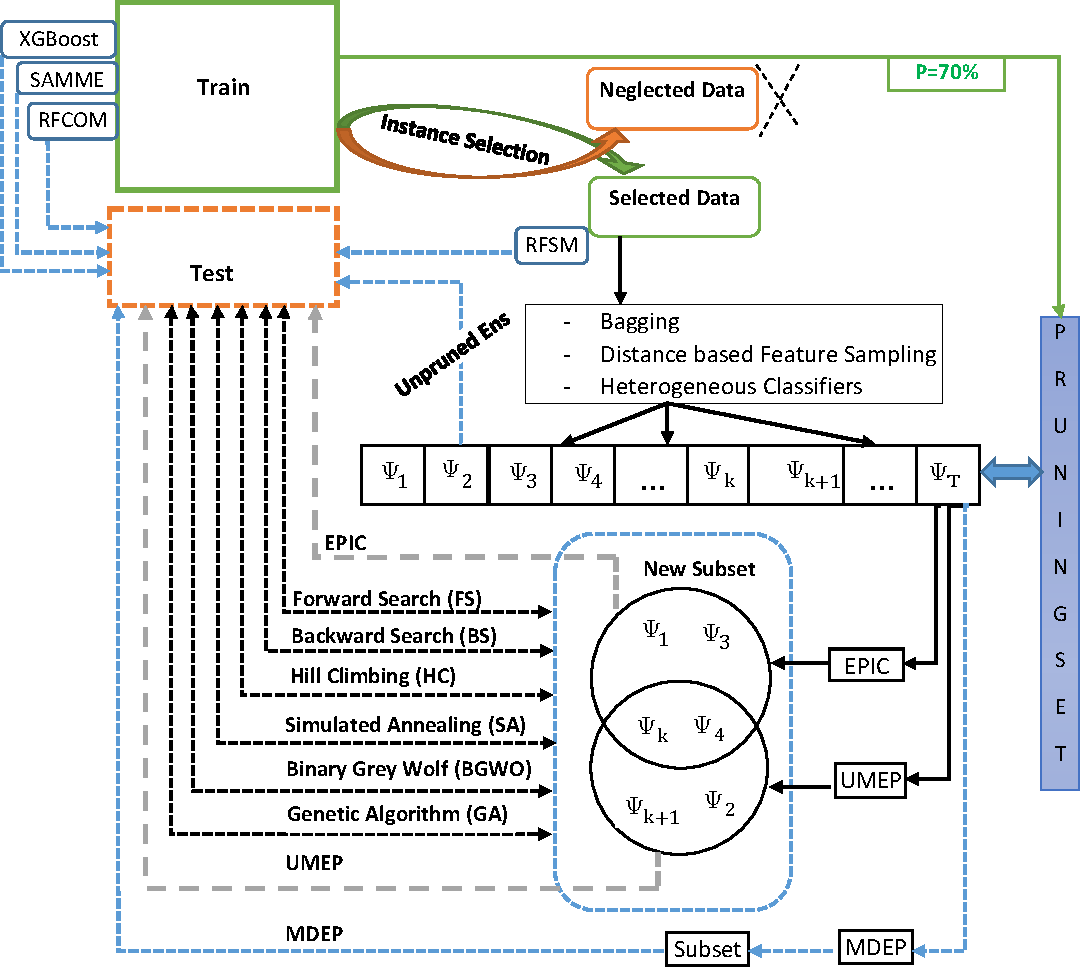
\includegraphics[width=.9\textwidth]{5_Guided_Search/fig/final-topology.pdf}
\caption{ The proposed ensemble selection in the presence of selected samples.}
\label{topology}
\end{figure*}


The two phases for cleaning noisy border samples, Section \ref{Training-set-selection}, and building heterogeneous MCS, Section \ref{proposed.mcs}, will not be changed. While we propose a guided search to prune the proposed ensemble. Therefore, we benefit from IS techniques and ensemble selection, rather than training large-size ensembles from large-size training data. 
   



\textbf{The Proposed Guided Search for Ensemble Pruning}: Having a large-size ensemble will limit the search capability of the well-known pruning metrics. As each pruning metric puts pressure to select a subset of classifiers with a specific property. For example, EPIC \cite{lu2010} concentrates on the classifier's diversity with the peer members. While UMEP \cite{guo2013} focuses more to select classifiers that behave well with low-margin samples. Regarding that, and with the large pool size of classifiers, the performance of the current pruning methods could vanish. Experimentally, Fig. \ref{conflicting} shows the generalized accuracy of the identified subensemble via different pruning methods, UMEP and EPIC, from different ensemble sizes. From Fig. \ref{conflicting}, we confirm that each metric is more important to a particular dataset. We conclude that paying no attention to other heuristic information affects the search process badly, and returns a subensemble with a limited accuracy.  

\vspace*{.3cm}
\begin{figure*}[h]
\begin{center}\scriptsize
  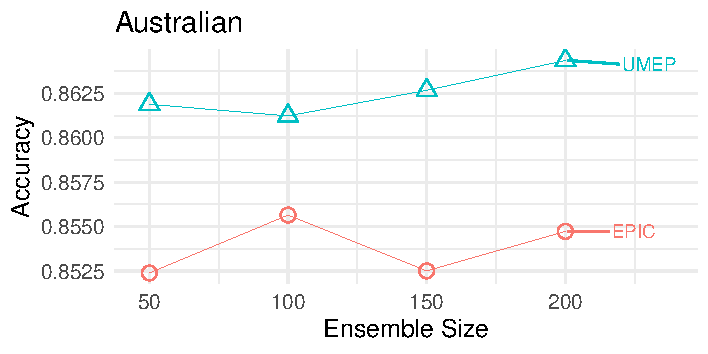
\includegraphics[width=.497\textwidth]{5_Guided_Search/fig/UMEP-EPIC-Australian.pdf}
  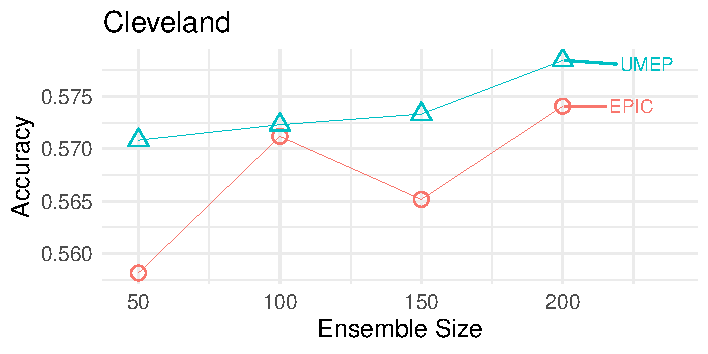
\includegraphics[width=.497\textwidth]{5_Guided_Search/fig/UMEP-EPIC-Cleveland.pdf}\\ 
  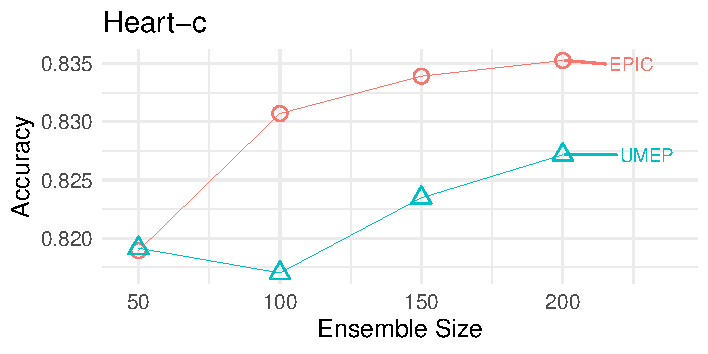
\includegraphics[width=.497\textwidth]{5_Guided_Search/fig/UMEP-EPIC-Heart-c.pdf}
   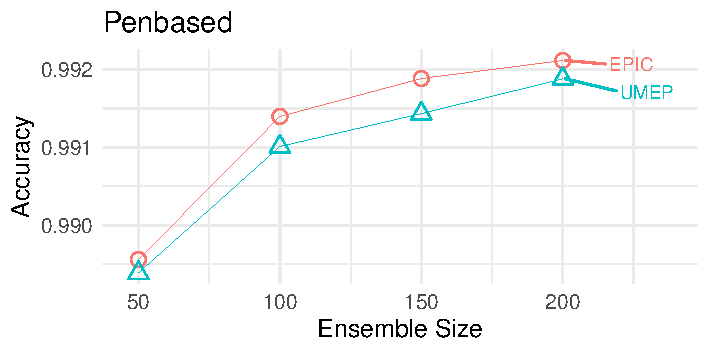
\includegraphics[width=.497\textwidth]{5_Guided_Search/fig/UMEP-EPIC-Penbased.pdf}\\
\end{center}
\caption{The conflict between both EPIC and UMEP, to be handled in this chapter.}
\label{conflicting}
\end{figure*}


Inspired by the above analysis, we can narrow the original search space by directing the search to promising areas. This is what EPIC and UMEP  return, each metric recommends a subspace according to their heuristic measures. Preferring one metric over the other will blinds a subspace that could contain crucial information. The two ordering-based pruning techniques, EPIC \cite{lu2010} and UMEP \cite{guo2013}, will be applied to determine the promising subspaces in advance. After that, the search process can be started. The details are as follows: 
 
 \begin{itemize}[nosep]
\item Each metric will rank the set of classifiers differently, but at least there will be common classifiers in-between.
 \item After ranking, a predetermined percentage, $P$, will be used to select a subset of classifiers. 
 \item A narrow space carrying the properties of both metrics will be formed via merging their output subsets, \textit{as in Fig. \ref{topology}}.
 \item The new subspace will be searched via Forward Search (FS) \footnote{Package Fselector:https://cran.r-project.org/web/packages/FSelector\label{fselect}}, Backward Search (BS)\textsuperscript{\ref{fselect}}, Hill Climbing (HC) \cite{cortez2014}, Simulated Annealing (SA) \cite{cortez2014}, Binary Grey Wolf Optimizer (BGWO) \cite{emary2016}, and Binary Genetic Algorithm (GA)\footnote{Package genalg:https://cran.r-project.org/web/packages/genalg}.    
 \end{itemize} 


Via guided search, we try to alleviate the randomness of the search process that could increase with large-size ensembles. To the best of our knowledge, this work is the first to handle the conflict between EPIC and UMEP. Moreover, it can be categorized as ensembling the pruning metrics themselves to get better performance than each of them.
%%%%%%%%%%%%%%%%%%%%%%%%%%%%%%%%%%%%%%%%%%%%%%%
%
%   Results
%
%%%%%%%%%%%%%%%%%%%%%%%%%%%%%%%%%%%%%%%%%%%%%%%
\section{Experimental Results}
\label{ch5_expsetup}
The experiments are dedicated to achieving objective 2, to increase the efficiency of MCS, and to go beyond what can be achieved from ensemble pruning methods. The two main questions to be answered are:
\begin{itemize}[nosep]
\setlength{\itemindent}{-.5in}
    \item $\pmb{Q_3}$. What is the effect of combining multiple pruning metrics together? 
    \item $\pmb{Q_4}$. What is the effect of downsizing data and downsizing the number of classifiers simultaneously? 
\end{itemize}

\subsection{Setup of Experiments}
During setup and validation, all datasets are preprocessed by unifying the scale of the features via normalization. For each dataset, 20 repetitions with 5 fold cross-validation procedure are considered. Thus, a total of 100 runs per dataset. The accuracy metric is calculated by the majority voting of all ensemble members. In addition, MDEP depends on an internal parameter $\alpha$; three values for MDEP with different $\alpha \in \{0.1, 0.5,0.9\}$ are considered, and the best-optimized alpha according to the in train-validation is used to report the test for each dataset separately.

A total number of 25 datasets captured from OpenML\footnote{ Machine Learning Repository: https://www.openml.org} and KEEL \footnote{KEEL Repository: http://www.keel.es/} are used in this work in order to provide experimentation. The characteristics of data can be found in Table \ref{ch5_data}, where \#S, \#F, \#C, and R represent the number of samples, the number of features, the number of classes, and the ratio between the smallest and the largest class for each dataset respectively. 


\vspace*{.3cm}
\begin{table}[!ht]
\centering\scriptsize
\caption{Characteristics of the selected datasets for experimentation, \textit{sorted by samples and classes}.}
 \label{ch5_data}
\resizebox{\textwidth}{!}{\begin{tabular}{l|cccc||l|cccc}
  \hline
\multicolumn{1}{c|}{DataSet} & \#S & \#F &  \#C & R  &DataSet & \#S & \#F &  \#C & R \\ 
  \hline
  Heart-statlog & 270 & 13 & 2 & 0.8 & Waveform & \numprint{4999} & 21 & 3 &  0.972 \\
   Heart-c & 303 & 13 & 2 & 0.836 & Cleveland & 297 & 13 &  5 & 0.081 \\ 
Ionosphere & 351 & 33 & 2 & 0.56 & Dermatology & 358 & 34 & 6 & 0.18 \\ 
  Sa-heart & 462 & 9 & 2 & 0.529 & Satimage & \numprint{6435} & 36 & 6 &  0.408 \\ 
  Wdbc & 569 & 30 & 2 &  0.594 & Segment & \numprint{2310} & 18 & 7 &  1.0 \\ 
  Breast-w & 699 & 9 & 2 &  0.526 & Mfeat-fourier & \numprint{2000} & 76 & 10  & 1.0 \\  
  Australian & 690 & 14 &  2 & 0.802 &  Mfeat-karh & \numprint{2000} & 64 & 10  & 1.0\\
  Blood-transfusion & 748 & 4 & 2 & 0.312  &Mfeat-zernike & \numprint{2000} & 47 & 10 & 1.0 \\   
  Mammographic & 830 & 5 & 2 & 0.944  & Led24 & \numprint{3200} & 24 & 10 & 0.878 \\  
 Diabetic Retinopathy & \numprint{1151} & 19 & 2 & 0.884  & Optdigits & \numprint{5620} & 62 & 10  & 0.969 \\
 Abalone & \numprint{4177} & 8 & 2 & 0.464   & Penbased & \numprint{10992} & 16 & 10  & 0.922 \\
 Ringnorm & \numprint{7400} & 20 & 2 & 0.981   & Texture & \numprint{5500} & 40 & 11 & 1.0 \\ 
 Twonorm &\numprint{7400} & 20 & 2 & 0.998 &  & & & & \\  
\hline
\end{tabular}
}
\label{dataset}
\end{table}







\subsection{Analysis of Guided Search} 
In this section, we concentrate on the performance of the proposed ensemble selection strategy. Table \ref{perAcc} shows the accuracy of subensemble related to percentage $P$ from the ensemble size $T$. Each row in Table \ref{perAcc} represents the average of 5,000 records of experiments (dataset=25 $\cdot$ runs=100 $\cdot$ $P$=2). From this table, the highest accuracy can be obtained by XGBoost, and  BS which merges EPIC and UMEP subspaces to exploit efficient classifiers. Moreover, the general accuracy is elevated as more classifiers are selected ($P$=20\%). It is interesting to observe that for $T=200$, SAMME, RFCOM, RFSM, and UNP realize an accuracy lower than 85.99\% that is reported by BS when it uses 12 classifiers. Regarding that, the proposed guided search from a low-size ensemble, $T=50$, cancels the necessity to initialize large-size ensembles. This could save huge training costs without losing the accuracy. 


The average subensemble size related to the predetermined $P$ value is shown in Table \ref{perSize}. Where FS guarantees to return a small-size subensemble, but unfortunately not accurate as shown in Table \ref{perAcc}. Furthermore, we can notice the performance of HC, SA, and BGWO according to both the accuracy and the subensemble size. The statistical analysis of the proposed pruning strategies shows that BS significantly outperforms the other five search methods (FS, HC, SA, BGWO, and GA) to identify a high accurate subensemble. Therefore, it is interesting to compare BS with EPIC, UMEP, and MDEP.
 
\vspace*{.3cm}






\begin{table}[!ht]
\centering\scriptsize
\caption{The average accuracy of subensemble related to selection percentage ($P$) of EPIC and UMEP, results over all datasets.}
\resizebox{\textwidth}{!}{\begin{tabular}{lccccc|ccccccccc|c}
  \hline
 \multicolumn{1}{c} { $T$} &\multicolumn{1}{c} {XGBoost} & SAMME & RFCOM & RFSM & UNP & EPIC & UMEP & MDEP &\multicolumn{1}{c} {FS} & BS & HC & SA & BGWO & GA & $P$ \\ 
  \hline   
\rule{0pt}{15pt}\multirow{2}{*}{50} & \multirow{2}{*}	{\textbf{ 86.60}} & \multirow{2}{*} {84.46} & \multirow{2}{*}{85.67} & \multirow{2}{*}{85.10} & \multirow{2}{*}{85.00} & 84.41 & 85.32 & 84.49 & 84.17 &\textbf{85.55} &85.34 & 85.29 & 85.40 & 83.38 & 10\% \\
&&&&&& 85.34 & 85.78 & 85.34 & 84.30 &\textbf{85.99} & 85.74 & 85.72 & 85.78 & 84.88 & 20\% \\ \hline
\rule{0pt}{15pt} \multirow{2}{*}{100}& \multirow{2}{*}	{\textbf{ 86.60}} & \multirow{2}{*}{84.88  } & \multirow{2}{*}{85.86} & \multirow{2}{*}{85.23} & \multirow{2}{*}{85.15} & 85.14 & 85.75 & 85.40 & 84.50 &\textbf{86.11} & 85.85 & 85.87 & 85.85 & 85.17 & 10\% \\
&&&&&& 85.94 & 86.12 & 85.97 & 84.61 & \textbf{86.33} & 86.14 & 86.14 & 86.15 & 85.65 & 20\% \\
    \hline   
    
\rule{0pt}{15pt}\multirow{2}{*}{150}& \multirow{2}{*}	{\textbf{ 86.53}} & \multirow{2}{*}{84.99 } & \multirow{2}{*}{85.95} & \multirow{2}{*}{85.28} & \multirow{2}{*}{85.23} & 85.46 & 86.13 & 85.81 & 84.72 &\textbf{86.28} & 86.11 & 86.12 & 86.09 & 85.47 & 10\%\\ 
&&&&&& 86.06 & 86.34 & 86.16 & 84.76 &\textbf{86.47} & 86.33 & 86.31 & 86.31 & 85.83 & 20\%\\ 
    \hline  
\rule{0pt}{15pt}\multirow{2}{*}{200} &\multirow{2}{*}	{\textbf{ 86.57}} & \multirow{2}{*}{85.06 } & \multirow{2}{*}{85.96} & \multirow{2}{*}{85.27} & \multirow{2}{*}{85.26} & 85.57 & 86.29 &85.93 & 84.68 &\textbf{86.41} & 86.28 & 86.24 & 86.18 & 85.71 & 10\% \\ 
&&&&&& 86.18 & 86.46 & 86.30 & 84.75 &\textbf{86.56} & 86.46 & 86.42 & 86.33 & 85.95 & 20\% \\ 
    \hline    
\end{tabular}}
\label{perAcc}
\end{table}

\vspace*{.3cm}
\begin{table}[!ht]
\centering\scriptsize
\caption{The average size of subensemble related to selection percentage ($P$) of EPIC and UMEP, results over all datasets.}
\resizebox{\textwidth}{!}{\begin{tabular}{lllll|ccccccccc|c}
  \hline
XGBoost &  SAMME & RFCOM & RFSM & UNP & EPIC &UMEP&MDEP &\multicolumn{1}{c} {FS} & BS & HC & SA & \multicolumn{1}{c} {BGWO} & GA & $P$ \\ 
 \cmidrule{1-6} \cmidrule(lr){6-8} \cmidrule(lr){9-15} 
\multicolumn{5}{c|}{\multirow{2}{*}{50}} & \multicolumn{3}{c}{5}  & \textbf{1.83} & 6.62 & 5.06 & 5.03  & 5.22  & 2.74  & 10\% \rule{0pt}{15pt} \\
\multicolumn{5}{c|}{}& \multicolumn{3}{c}{10} &\textbf{2.06} & 12.37  & 8.00 & 7.89 &7.89 & 4.77 & 20\% \\ \hline

\multicolumn{5}{c|}{\multirow{2}{*}{100}} & \multicolumn{3}{c}{10}  &\textbf{2.13} & 13.69 & 8.55 & 8.48  & 8.41 & 5.03  & 10\% \rule{0pt}{15pt} \\
\multicolumn{5}{c|}{}  & \multicolumn{3}{c}{20} &\textbf{2.31}  & 25.90 & 14.30 & 14.42 & 13.19 & 6.74 & 20\%  \\ \hline

\multicolumn{5}{c|}{\multirow{2}{*}{150}} & \multicolumn{3}{c}{15}  & \textbf{2.32} & 20.99 & 12.01 & 12.06  & 11.35  & 6.13  & 10\% \rule{0pt}{15pt} \\
\multicolumn{5}{c|}{} & \multicolumn{3}{c}{30} &\textbf{2.50}  &39.69 & 20.94 & 20.84 & 18.54 & 7.95  & 20\%  \\ \hline

\multicolumn{5}{c|}{\multirow{2}{*}{200}} & \multicolumn{3}{c}{20}  & \textbf{2.41} & 28.54 & 15.56 & 15.59  & 12.49  & 6.86  & 10\%  \rule{0pt}{15pt}\\
\multicolumn{5}{c|}{}  & \multicolumn{3}{c}{40} &\textbf{2.55} &53.55 & 27.54 & 27.65 & 19.37 & 8.98 & 20\% \\ \hline

\end{tabular}}
\label{perSize}
\end{table}





\afterpage{
\begin{landscape}
\begin{table}[!ht]
\caption{Classification accuracy of BS, EPIC, UMEP, and MDEP for selecting subensemble from $T=200$ model, the best value is in bold.}
\label{BS-EPIC-UMEP}
\centering\scriptsize
\renewcommand{\arraystretch}{1.3}
\begin{adjustbox}{max width=1.5\textwidth}
\begin{tabular}{llcccc|cccc}
\hline
 \#& Dataset & \multicolumn{1}{c}{BS-10} & EPIC-10\% & UMEP-10\% & MDEP-10\% & \multicolumn{1}{c}{BS-20} & EPIC-20\% & UMEP-20\% & MDEP-20\% \\ 
  \hline
\rule{0pt}{10pt}  $D_{1}$ & Abalone & 69.88 $\pm$ 1.21 & 66.73 $\pm$ 2.39 & 69.83 $\pm$ 1.04 &69.78 $\pm$ 1.12& \textbf{70.04 $\pm$ 1.14} & 68.11 $\pm$ 1.80 & 69.85  $\pm$ 1.00 & 69.96 $\pm$ 1.12\\
\rule{0pt}{10pt}  $D_{2}$ & Australian & 86.58 $\pm$ 2.47 & 84.60 $\pm$  3.17 & \textbf{86.59 $\pm$ 2.65} &86.37 $\pm$ 2.76& 86.50  $\pm$ 2.60 & 85.47  $\pm$ 2.62 & 86.43  $\pm$ 2.65 & 86.25 $\pm$ 2.80 \\ 
\rule{0pt}{10pt}  $D_{3}$ & Blood-transfusion & 77.19 $\pm$ 2.30 & 73.88 $\pm$ 4.73 & 77.00 $\pm$ 2.40 &76.51 $\pm$ 2.61& \textbf{77.64  $\pm$ 2.22}& 76.22  $\pm$ 3.65& 77.17  $\pm$ 2.08&77.22 $\pm$ 2.08 \\ 
\rule{0pt}{10pt}  $D_{4}$ & breast-w & 96.99 $\pm$ 1.20 & 96.63 $\pm$ 1.39 &96.99 $\pm$ 1.28 &97.00 $\pm$ 1.40& 97.12 $\pm$ 1.23& 96.87 $\pm$ 1.30& \textbf{97.13 $\pm$ 1.25}& \textbf{97.13 $\pm$ 1.31}\\ 
\rule{0pt}{10pt}  $D_{5}$ & Cleveland & 57.25 $\pm$ 4.27 & 54.98 $\pm$ 5.84 & 57.52 $\pm$ 3.41 &57.06 $\pm$ 3.43& \textbf{57.96 $\pm$ 3.66}&57.41 $\pm$ 4.27& 57.84 $\pm$ 3.12& 57.56 $\pm$ 3.10\\ 
\rule{0pt}{10pt}  $D_{6}$ & Dermatology & \textbf{97.63 $\pm$ 1.69} & 97.40 $\pm$ 1.79 & 97.50 $\pm$ 1.80&97.49 $\pm$ 1.74 & 97.53  $\pm$ 1.72 & 97.32 $\pm$ 1.89 & 97.56 $\pm$ 1.62& \textbf{97.63 $\pm$ 1.65} \\ 
\rule{0pt}{10pt}  $D_{7}$ & Diabetic  & 70.77 $\pm$ 2.99 & 69.71 $\pm$ 2.59 &\textbf{70.89 $\pm$ 3.28} &70.71 $\pm$ 2.96&69.81 $\pm$ 3.10& 69.63 $\pm$ 2.75& 70.26 $\pm$ 3.20&70.49 $\pm$ 3.00\\ 
\rule{0pt}{10pt}  $D_{8}$ & Heart-c & 82.83 $\pm$ 4.55& 82.75 $\pm$ 4.38 & 82.25 $\pm$ 4.76 &82.06 $\pm$ 4.68& \textbf{83.61 $\pm$ 4.26}& 83.53 $\pm$ 4.25& 82.72 $\pm$ 4.58& 83.12 $\pm$ 4.33\\  
\rule{0pt}{10pt}  $D_{9}$ & Heart-statlog & 83.02 $\pm$ 4.29 & 81.13 $\pm$ 4.14& 82.94 $\pm$ 4.21 &83.24 $\pm$ 4.29&83.46 $\pm$ 4.27& 82.57 $\pm$ 4.45& 83.11 $\pm$ 4.07&\textbf{83.70 $\pm$ 4.26}\\ 
\rule{0pt}{10pt}  $D_{10}$ & Ionosphere & \textbf{92.54 $\pm$ 2.85}& 92.07 $\pm$ 2.83& 91.67 $\pm$ 3.09 &92.14 $\pm$ 2.59& 92.34 $\pm$ 2.75& 92.41 $\pm$ 2.61& 91.93 $\pm$ 2.89&92.49 $\pm$ 2.74\\ 
\rule{0pt}{10pt}  $D_{11}$ & Led24 & 71.62 $\pm$ 1.54& 71.16 $\pm$ 1.74& 71.58 $\pm$ 1.51&65.89 $\pm$ 4.76& \textbf{71.89 $\pm$ 1.45}& 71.75 $\pm$ 1.46& 71.78 $\pm$ 1.45&68.66 $\pm$ 3.79\\ 
\rule{0pt}{10pt}  $D_{12}$ & Mammographic & 83.76 $\pm$ 2.51& 83.05 $\pm$ 2.55& 83.72 $\pm$ 2.54 &83.56 $\pm$ 2.47& 83.89 $\pm$ 2.36& 83.37 $\pm$ 2.64&84.00 $\pm$ 2.32&\textbf{84.05 $\pm$ 2.27}\\  
\rule{0pt}{10pt}  $D_{13}$ & Mfeat-fourier & \textbf{81.41 $\pm$ 1.55}& 80.34 $\pm$ 1.76& 80.97 $\pm$ 1.62&80.41 $\pm$ 1.67& \textbf{81.41 $\pm$ 1.62}& 80.89 $\pm$ 1.65& 81.34 $\pm$ 1.56&81.12 $\pm$ 1.63\\ 
\rule{0pt}{10pt}  $D_{14}$ & Mfeat-karh &96.08 $\pm$ 0.88& 95.67 $\pm$ 0.99& 96.05 $\pm$ 0.86 &95.99 $\pm$ 1.13&\textbf{96.31 $\pm$ 0.89}& 96.19 $\pm$ 0.86& 96.27 $\pm$ 0.85&96.28 $\pm$ 0.96\\ 
\rule{0pt}{10pt}  $D_{15}$ & Mfeat-zernike & 82.05 $\pm$ 1.47& 81.94 $\pm$ 1.58&82.08 $\pm$ 1.49 &81.49 $\pm$ 1.58& 82.38 $\pm$ 1.39& 82.19 $\pm$ 1.52& \textbf{82.48 $\pm$ 1.44}&82.20 $\pm$ 1.41\\ 
\rule{0pt}{10pt}  $D_{16}$ & Optdigits & 98.53 $\pm$ 0.32& 98.50 $\pm$ 0.34& 98.54 $\pm$ 0.34 &98.53 $\pm$ 0.34&\textbf{ 98.61 $\pm$ 0.32}& \textbf{98.61 $\pm$ 0.31}& 98.60 $\pm$ 0.31&98.59 $\pm$ 0.30\\ 
\rule{0pt}{10pt}  $D_{17}$ & Penbased & 99.15 $\pm$ 0.19& 99.15 $\pm$ 0.18& 99.10 $\pm$ 0.19 &99.03 $\pm$ 0.71& 99.20 $\pm$ 0.16& \textbf{99.21 $\pm$ 0.16}& 99.19 $\pm$ 0.17&99.10 $\pm$ 0.69\\ 
\rule{0pt}{10pt}  $D_{18}$ & Ringnorm & 96.36 $\pm$ 0.54& 95.94 $\pm$ 0.55& 95.92 $\pm$ 0.56 &96.00 $\pm$ 0.51& \textbf{96.50 $\pm$ 0.48}& 96.33 $\pm$ 0.51& 96.33 $\pm$ 0.51&96.37 $\pm$ 0.49\\ 
 \rule{0pt}{10pt} $D_{19}$ & Sa-heart &70.49 $\pm$ 4.17& 69.44 $\pm$ 4.33& 70.64 $\pm$ 3.90 &70.47 $\pm$ 3.53& 70.98 $\pm$ 4.06& 70.50 $\pm$ 4.30& 70.98 $\pm$ 3.86&\textbf{71.25 $\pm$ 3.65}\\ 
 \rule{0pt}{10pt} $D_{20}$ & Satimage & 90.12 $\pm$ 0.78& 90.04 $\pm$ 0.80& 90.00 $\pm$ 0.81&89.70 $\pm$ 1.46& 90.16 $\pm$ 0.72& \textbf{90.17 $\pm$ 0.75}& 90.05 $\pm$ 0.77&89.81 $\pm$ 1.39\\ 
 \rule{0pt}{10pt} $D_{21}$ & Segment & 96.56 $\pm$ 0.74& 96.34 $\pm$ 0.74& 96.41 $\pm$ 0.69 &96.20 $\pm$ 1.02& \textbf{96.61 $\pm$ 0.77}& \textbf{96.61 $\pm$ 0.77}& 96.54 $\pm$ 0.74&96.51 $\pm$ 0.87\\ 
\rule{0pt}{10pt}  $D_{22}$ & Texture & 99.62 $\pm$ 0.20& 99.61 $\pm$ 0.20& 99.60 $\pm$ 0.19 &99.62 $\pm$ 0.18&\textbf{99.63 $\pm$ 0.18}& \textbf{99.63 $\pm$ 0.19}&\textbf{99.63 $\pm$ 0.19}&\textbf{99.63 $\pm$ 0.16}\\  
\rule{0pt}{10pt}  $D_{23}$ & Twonorm &97.31 $\pm$ 0.40& 97.04 $\pm$ 0.42& 97.14 $\pm$ 0.41 &97.09 $\pm$ 0.45& \textbf{97.55 $\pm$ 0.35}& 97.38 $\pm$ 0.39& 97.46 $\pm$ 0.38&97.47 $\pm$ 0.42\\ 
\rule{0pt}{10pt}  $D_{24}$ & Waveform & 85.04 $\pm$ 0.94& 83.82 $\pm$ 0.98& 84.95 $\pm$ 1.0 &84.82 $\pm$ 1.13& \textbf{85.42 $\pm$ 0.93} & 84.59 $\pm$ 1.00&85.41 $\pm$ 0.95&85.34 $\pm$ 1.07\\ 
 \rule{0pt}{10pt} $D_{25}$ & Wdbc & 97.42 $\pm$ 1.66& 97.34 $\pm$ 1.68& 97.35 $\pm$ 1.68 &97.16 $\pm$ 1.58& 97.49 $\pm$ 1.56& \textbf{97.52 $\pm$ 1.46}&97.48 $\pm$ 1.63&97.34 $\pm$ 1.58\\ 
   \hline
  \multicolumn{2}{c}{\textbf{AR-Friedman}}&\multicolumn{1}{c}{\textbf{3.92}}&\multicolumn{1}{c} {7.16} &\multicolumn{1}{c}{5.32} &\multicolumn{1}{c}{ 6.36} & \multicolumn{1}{c}{\textbf{2.06}}&\multicolumn{1}{c}{ 4.56} &\multicolumn{1}{c}{ 3.32} &\multicolumn{1}{c}{ 3.3}  \rule{0pt}{10pt} \\ 
   \hline

\end{tabular}
\end{adjustbox}
\end{table}
\end{landscape}
}


\textbf{To answer} $\pmb{Q_3}$, Table \ref{BS-EPIC-UMEP} illustrates the average accuracy and standard deviation via BS, EPIC, UMEP, and MDEP for 100 runs per dataset. As shown, BS obtains the best average rankings by Friedman Test \cite{demsar2006}, \textit{AR-Friedman}, to select an effective subensemble. EPIC-10\%, UMEP-10\%, and MDEP-10\% return a subensemble with 20 classifiers, while BS-10 returns a large-size subensemble, as demonstrated in Table. \ref{perSize}. While the size and the accuracy of the subensemble are important, Table \ref{Acc-size} shows the pairwise statistical analysis \cite{wilcoxon1945} for calibration between them. From Table \ref{Acc-size}, BS-10 is comparable with EPIC-20\%, UMEP-20\%, and MDEP-20\% in terms of accuracy, however, it significantly outperforms them regarding the subensemble size. Furthermore, the obtained subensemble's accuracy by BS-20 significantly outperforms all the pruning methods, this is marked by ($\blacktriangle$). The user has more flexibility to prefer a high accurate subensemble ($\blacktriangle$), the lower part of the table, or to prefer a small-size subensemble (\textbullet) as in the upper part. 
\vspace*{.3cm}


\begin{table*}[!ht]
\centering\scriptsize
\caption{Summary of the Wilcoxon test. Shape denotes the measure used, accuracy ($\blacktriangle$ $\triangle$) and size (\textbullet \textopenbullet). The filled shape ($\blacktriangle$ \textbullet) represents if the method in the row outperforms the one in the column or vice versa for ($\triangle$ \textopenbullet). Upper diagonal of level significance $\alpha=0.9$, lower diagonal level of significance $\alpha=0.95$.}

\renewcommand{\arraystretch}{1.3}
\begin{tabular}{
|l|c|c|c|c|c|c|c|c|}
\hline
&(1) &(2) &(3) & (4)&(5) &(6) &(7)&(8) \\
\hline
BS-10 (1)& - -& $\blacktriangle $ \textopenbullet & $\blacktriangle$ \textopenbullet &$\blacktriangle$ \textopenbullet & $\triangle$ \textbullet & \textbullet & \textbullet& \textbullet\\
\hline
EPIC-10\% (2)& $\triangle$ \textbullet & - - & $\triangle$ &$\triangle$ & $\triangle$ \textbullet& $\triangle$ \textbullet& $\triangle$ \textbullet&$\triangle$ \textbullet \\
\hline
UMEP-10\% (3)& $\triangle$ \textbullet & $\blacktriangle$ &- -&$\blacktriangle $ & $\triangle$ \textbullet & \textbullet & $\triangle$ \textbullet & $\triangle$ \textbullet\\
\hline
MDEP-10\% (4)& $\triangle$ \textbullet &  &$\triangle$ &- - & $\triangle$ \textbullet &  \textbullet&$\triangle$ \textbullet  &$\triangle$ \textbullet \\
\hline
BS-20 (5)& $\blacktriangle$ \textopenbullet & $\blacktriangle$ \textopenbullet & $\blacktriangle$ \textopenbullet&$\blacktriangle$ \textopenbullet &- -& $\blacktriangle$ \textopenbullet & $\blacktriangle$ \textopenbullet& $\blacktriangle$ \textopenbullet\\
\hline
EPIC-20\% (6)& \textopenbullet & $\blacktriangle$ \textopenbullet& \textopenbullet & \textopenbullet& $\triangle$ \textbullet &- -& $\triangle$ &$\triangle$\\
\hline
UMEP-20\% (7)& \textopenbullet & $\blacktriangle$ \textopenbullet & $\blacktriangle$ \textopenbullet &$\blacktriangle$ \textopenbullet&$\triangle$ \textbullet &$\blacktriangle$  &- -&\\
\hline
MDEP-20\% (8)& \textopenbullet & $\blacktriangle$ \textopenbullet & $\blacktriangle$ \textopenbullet& $\blacktriangle$\textopenbullet& \textbullet &$\blacktriangle$  &  &- - \\
\hline
\end{tabular}
\label{Acc-size}
\end{table*}

 
\subsection{Classification Performance of the Proposed Method}\label{LFRD}



\afterpage{
\begin{landscape}
\begin{table}[!ht]
        \centering \scriptsize
\caption{Average accuracy and standard deviation of NRD-NSE, RD-NSE, and RD-SE from ensemble size $T= 200$. The best value is in bold, while the second best is underlined.}
\label{ch5_complete-table}
\renewcommand{\arraystretch}{1.9}
\begin{adjustbox}{max width=1.5\textwidth} \begin{tabular}{llccccccccccccccc}
  \hline
   & & AllKNN &\multicolumn{3}{c}{NRD-NSE}&\multicolumn{2}{c}{RD-NSE}&\multicolumn{9}{c}{RD-SE}\\
 \cmidrule(lr){3-3} \cmidrule(lr){4-6} \cmidrule(lr){7-8} \cmidrule(lr){9-17}
 \#&  Dataset & Red\_Rate & XGBoost &SAMME & RFCOM & \multicolumn{1}{c}{RFSM} & \multicolumn{1}{c}{UNP} & \multicolumn{1}{c}{EPIC} & \multicolumn{1}{c}{UMEP} &
 \multicolumn{1}{c}{MDEP} &
 \multicolumn{1}{c}{FS} & \multicolumn{1}{c}{BS} & \multicolumn{1}{c}{HC} & \multicolumn{1}{c}{SA} & \multicolumn{1}{c}{BGWO} & \multicolumn{1}{c}{GA} \\ 
\hline
$D_1$ & Abalone & 0.47 & 69.05$\pm$ 1.29 & 69.67 $\pm$ 1.21 & 69.11 $\pm$ 1.27 & 69.99 $\pm$ 1.07  & 69.52 $\pm$ 0.64 & 68.11 $\pm$ 1.80 & 69.85 $\pm$ 1.00 & 69.96 $\pm$ 1.12 & 68.60 $\pm$ 1.46   & \textbf{70.04 $\pm$ 1.14} & 69.90 $\pm$ 1.12 & \underline{70.00 $\pm$ 1.19} & 69.81 $\pm$ 1.10 & 69.58 $\pm$ 1.12 \\ 
  $D_2$ & Australian & 0.26 &\textbf{ 87.22 $\pm$ 2.60} & 86.50 $\pm$ 2.36 &\underline{87.12 $\pm$ 2.56} & 86.33 $\pm$ 2.58  & 86.05 $\pm$ 2.46 & 85.47 $\pm$ 2.62 & 86.43 $\pm$ 2.65 & 86.25 $\pm$ 2.80 & 86.17 $\pm$  2.53  & 86.50 $\pm$ 2.60 & 86.64 $\pm$ 2.42  & 86.60 $\pm$ 2.45 & 86.44 $\pm$ 2.51 & 86.10 $\pm$ 2.68 \\ 
  $D_3$ & Blood-transfusion & 0.49 &77.55 $\pm$ 2.25 & 74.50 $\pm$ 2.60 & 75.51 $\pm$ 2.43 & 77.22 $\pm$ 2.60 & 76.90 $\pm$ 1.45 & 76.22 $\pm$ 3.65 & 77.17 $\pm$ 2.08 &77.22 $\pm$ 2.08 & 77.23 $\pm$ 2.35  & 77.64 $\pm$ 2.22 & \textbf{77.79 $\pm$ 2.16} & \underline{77.75 $\pm$ 2.19} & 77.51 $\pm$ 1.97 & 77.31 $\pm$ 2.36 \\ 
  $D_4$ & Breast-w & 0.06 & 96.55 $\pm$ 1.38 & 96.88 $\pm$ 1.19 & 97.09 $\pm$ 1.22 & 96.61 $\pm$ 1.39 & \textbf{97.42 $\pm$ 1.17}  & 96.87 $\pm$ 1.30 & \underline{97.13 $\pm$ 1.25} &\underline{97.13 $\pm$ 1.31} & 96.11 $\pm$ 1.55  & 97.12 $\pm$ 1.23  & 97.07 $\pm$ 1.28  & 97.09 $\pm$ 1.24  & 97.02 $\pm$ 1.17 & 96.78 $\pm$ 1.35 \\ 
  $D_5$ & Cleveland & 0.55 &56.15 $\pm$ 4.30 & 53.02 $\pm$ 5.11 & 57.14 $\pm$ 3.75 & 56.49 $\pm$  2.79 & 56.50 $\pm$ 2.88 &57.41 $\pm$ 4.27 & 57.84 $\pm$ 3.12 & 57.56 $\pm$ 3.10 & 56.39 $\pm$ 3.82 &\textbf{57.96 $\pm$ 3.66}  & 57.74 $\pm$ 3.60 & 57.51 $\pm$ 3.72 & \underline{57.86 $\pm$ 3.30} & 57.20 $\pm$ 3.85 \\ 
  $D_6$ & Dermatology & 0.07 &\textbf{97.96 $\pm$ 1.57} & 96.69 $\pm$ 1.77 & 97.45 $\pm$ 1.55 & 97.44 $\pm$ 1.46 & 97.46 $\pm$ 1.65 & 97.32 $\pm$ 1.89 & 97.56 $\pm$ 1.62 & \underline{97.63 $\pm$ 1.65} & 96.00 $\pm$ 2.22 & 97.53 $\pm$ 1.72& 97.53 $\pm$ 1.61 & 97.61 $\pm$ 1.76 & 97.26 $\pm$ 1.80 & 96.64 $\pm$ 1.95 \\ 
  $D_7$ & Diabetic & 0.55 &68.99 $\pm$ 2.55 & 69.14 $\pm$ 2.76 & 67.86 $\pm$ 2.82 & 65.83 $\pm$ 2.82 & 66.38 $\pm$ 2.94 & 69.63 $\pm$ 2.75  & 70.26 $\pm$ 3.20 &\underline{70.49 $\pm$ 3.00}&\textbf{ 70.90 $\pm$ 3.15} & 69.81 $\pm$ 3.10 & 69.97 $\pm$ 3.13 & 69.80 $\pm$ 3.02 & 70.08 $\pm$ 3.07 & 70.19 $\pm$ 3.34 \\ 
  $D_8$ & Heart-c & 0.32 & \textbf{83.85 $\pm$ 4.96} & 79.88 $\pm$ 4.75 & 83.00 $\pm$ 4.60 & 82.18 $\pm$ 4.35  & 83.22 $\pm$ 4.49 & 83.53 $\pm$ 4.25 & 82.72 $\pm$ 4.58 & 83.12 $\pm$ 4.33 & 79.91 $\pm$ 4.99 & \underline{83.61 $\pm$ 4.26} & 83.59 $\pm$ 4.37 & 83.22 $\pm$ 4.64 & 83.39 $\pm$ 4.24 & 82.21 $\pm$ 4.62 \\ 
  $D_9$ & Heart-statlog & 0.34 & \textbf{83.93 $\pm$ 4.40}& 79.28 $\pm$ 5.02 & 82.78 $\pm$ 4.34 & 81.30 $\pm$ 4.99 & 83.07 $\pm$ 4.71 & 82.57 $\pm$ 4.45 & 83.11 $\pm$ 4.07 &\underline{83.70 $\pm$ 4.26}& 80.35 $\pm$ 5.14 & 83.46 $\pm$ 4.27 & 83.31 $\pm$ 4.32 & 83.33 $\pm$ 4.24 & 82.78 $\pm$  4.42 & 82.67 $\pm$ 3.92 \\ 
  $D_{10}$ & Ionosphere & 0.19 &92.95 $\pm$ 3.02& \textbf{93.70 $\pm$ 2.26} & \underline{93.26 $\pm$ 2.53} & 91.08 $\pm$ 2.75 & 89.67 $\pm$ 2.98 & 92.41 $\pm$ 2.61  & 91.93 $\pm$ 2.89 &92.49 $\pm$ 2.74& 90.69 $\pm$ 3.53 & 92.34 $\pm$ 2.75 & 92.44 $\pm$ 2.94 & 92.25 $\pm$ 2.75 & 92.34 $\pm$ 2.88 & 92.21 $\pm$ 2.86 \\ 
  $D_{11}$ & Led24 & 0.68 &\textbf{72.56 $\pm$ 1.43}& 66.40 $\pm$ 1.41 &\underline{72.21 $\pm$ 1.40} & 71.55 $\pm$ 1.63 & 70.02 $\pm$ 1.76 & 71.75 $\pm$ 1.46 & 71.78 $\pm$ 1.45 &68.66 $\pm$ 3.79& 70.38 $\pm$ 2.23 & 71.89 $\pm$ 1.45 & 71.75 $\pm$ 1.58 & 71.73 $\pm$ 1.51 & 71.72 $\pm$ 1.55 & 71.29 $\pm$ 1.58 \\ 
  $D_{12}$ & Mammographic & 0.35 &82.56 $\pm$ 2.66& 79.81 $\pm$ 2.36 & 81.76 $\pm$ 2.49 & 82.20 $\pm$ 2.43 & 82.06 $\pm$ 2.51 & 83.37 $\pm$ 2.64 & \underline{84.00 $\pm$ 2.32} &\textbf{84.05 $\pm$ 2.27}& 82.96 $\pm$ 2.77 & 83.89 $\pm$ 2.36 & 83.67 $\pm$ 2.45 & 83.73 $\pm$ 2.44 & 83.57 $\pm$ 2.45 & 83.39 $\pm$ 2.39 \\ 
  $D_{13}$ & Mfeat-fourier & 0.28 &\textbf{83.47 $\pm$ 1.86}& 82.33 $\pm$ 1.64 &\underline{ 83.07 $\pm$ 1.53} & 80.45 $\pm$  1.52 & 80.14 $\pm$ 1.50 & 80.89 $\pm$ 1.65 & 81.34 $\pm$ 1.56 &81.12 $\pm$ 1.63& 76.67 $\pm$ 2.46 & 81.41 $\pm$ 1.62 & 80.91 $\pm$ 1.63 & 80.96 $\pm$ 1.77 & 80.68 $\pm$ 1.57 & 79.89 $\pm$ 1.88 \\ 
  $D_{14}$ & Mfeat-karh & 0.07 &95.28 $\pm$ 0.99& 96.09 $\pm$ 0.95 & 96.25 $\pm$ 0.87& 95.46 $\pm$ 0.94 & 96.13 $\pm$ 0.88 & 96.19 $\pm$ 0.86 & 96.27 $\pm$ 0.85 &\underline{96.28 $\pm$ 0.96}&92.14 $\pm$ 2.14 &\textbf{96.31 $\pm$ 0.89}& 96.06 $\pm$ 0.87 & 96.06 $\pm$ 0.86 & 95.77 $\pm$ 1.00 & 95.23 $\pm$ 0.98 \\ 
  $D_{15}$ & Mfeat-zernike & 0.26 &81.73 $\pm$ 1.52& 80.12 $\pm$ 1.65 & 77.87 $\pm$ 1.49 & 76.20 $\pm$ 1.45 & 80.72 $\pm$ 1.24 & 82.19 $\pm$ 1.52 & \textbf{82.48 $\pm$ 1.44} &82.20 $\pm$ 1.41& 78.22  $\pm$ 2.28 &\underline{ 82.38 $\pm$ 1.39}& 82.20 $\pm$ 1.37 & 82.14 $\pm$ 1.35 & 81.92 $\pm$ 1.40 & 81.58 $\pm$ 1.57 \\ 
  $D_{16}$ & Optdigits & 0.02 &98.13 $\pm$ 0.39& 98.14 $\pm$ 0.36 & 98.32 $\pm$ 0.35 & 98.00 $\pm$ 0.38 & 98.09 $\pm$ 0.38 & \textbf{98.61 $\pm$ 0.31} &\underline{98.60 $\pm$ 0.31} &98.59 $\pm$ 0.30& 97.14 $\pm$ 0.66 & \textbf{98.61 $\pm$ 0.32} & 98.51 $\pm$ 0.34 & 98.51 $\pm$ 0.34 & 98.42 $\pm$ 0.41 & 98.10 $\pm$ 0.49 \\ 
  $D_{17}$ & Penbased & 0.01 &99.13 $\pm$ 0.20& 98.73 $\pm$ 0.26 & 99.16 $\pm$ 0.19 & 99.01 $\pm$ 0.20 & 98.22 $\pm$ 0.27 & \textbf{99.21 $\pm$ 0.16} & 99.19 $\pm$ 0.17 &99.10 $\pm$ 0.69& 97.57 $\pm$ 0.62 & \underline{99.20 $\pm$ 0.16} & 99.14 $\pm$ 0.18 & 99.15 $\pm$ 0.16 & 99.12 $\pm$ 0.19 & 98.93 $\pm$ 0.25 \\ 
  $D_{18}$ & Ringnorm & 0.32 &\underline{96.67 $\pm$ 0.41}& \textbf{97.24 $\pm$ 0.36} & 95.04 $\pm$ 0.56 & 93.09 $\pm$ 0.78 & 86.69 $\pm$ 1.15 & 96.33 $\pm$ 0.51 & 96.33 $\pm$ 0.51 &96.37 $\pm$ 0.49& 92.89 $\pm$ 0.63 & 96.50 $\pm$ 0.48 & 96.43 $\pm$ 0.48 & 96.32 $\pm$ 0.49 & 96.43 $\pm$ 0.49 & 95.89 $\pm$ 0.80 \\ 
  $D_{19}$ & Sa-heart & 0.49 &\textbf{72.82 $\pm$ 3.75}& 64.57 $\pm$ 4.28 & 68.83 $\pm$ 4.14 & 70.57 $\pm$ 4.03 &\underline{71.41 $\pm$ 3.77} & 70.50 $\pm$ 4.30 & 70.98 $\pm$ 3.86 &71.25 $\pm$ 3.65&69.29 $\pm$ 4.29 & 70.98 $\pm$ 4.06 & 70.67 $\pm$ 3.91 & 70.72 $\pm$ 4.05 & 70.38 $\pm$ 4.13 & 70.07 $\pm$ 4.24 \\ 
  $D_{20}$ & Satimage & 0.14&\textbf{92.08 $\pm$ 0.67}& 88.72 $\pm$ 0.78 &\underline{ 91.71 $\pm$ 0.71} & 89.84 $\pm$ 0.71 & 88.70 $\pm$ 0.78 & 90.17 $\pm$ 0.75 & 90.05 $\pm$ 0.77 &89.81 $\pm$ 1.39& 89.76 $\pm$ 0.80 & 90.16 $\pm$ 0.72 & 90.10 $\pm$ 0.74 & 90.12 $\pm$ 0.74 & 89.96 $\pm$ 0.77 & 89.67 $\pm$ 0.72 \\ 
  $D_{21}$ & Segment & 0.06 &\underline{98.08 $\pm$ 0.67}& \textbf{98.43 $\pm$ 0.60} & 97.89 $\pm$ 0.69 & 96.53 $\pm$ 0.83 & 95.94 $\pm$ 0.90 & 96.61 $\pm$ 0.77 & 96.54 $\pm$ 0.74 &96.51 $\pm$ 0.87& 94.92 $\pm$ 1.38 & 96.61 $\pm$ 0.77 & 96.57 $\pm$ 0.80 & 96.59 $\pm$ 0.84 & 96.69 $\pm$ 0.87 & 96.44 $\pm$ 0.90 \\ 
  $D_{22}$ & Texture & 0.02 &98.37 $\pm$ 0.38& 98.56 $\pm$ 0.40 & 97.77 $\pm$ 0.47 & 97.14 $\pm$ 0.50 & 98.40 $\pm$ 0.35 & \textbf{99.63 $\pm$ 0.19} & \textbf{99.63 $\pm$ 0.19} &\textbf{99.63 $\pm$ 0.16}& 99.27 $\pm$ 0.39 & \textbf{99.63 $\pm$ 0.18} & 99.59 $\pm$ 0.21 & \underline{99.60 $\pm$ 0.21} & \underline{99.60 $\pm$ 0.21} & 99.52 $\pm$ 0.25 \\ 
  $D_{23}$ & Twonorm & 0.08 &97.29 $\pm$ 0.38& 97.31 $\pm$ 0.38 & 97.23 $\pm$ 0.41 & 97.12 $\pm$ 0.39 &\textbf{ 97.69 $\pm$ 0.37}& 97.38 $\pm$ 0.39 & 97.46 $\pm$ 0.38 &97.47 $\pm$ 0.42& 94.85 $\pm$ 1.41 &\underline{ 97.55 $\pm$ 0.35} & 97.38 $\pm$ 0.40 & 97.35 $\pm$ 0.41 & 97.25 $\pm$ 0.43 & 96.86 $\pm$ 0.48 \\ 
  $D_{24}$ & Waveform & 0.32 &85.24 $\pm$ 1.05& 83.43 $\pm$ 1.05 & 85.39 $\pm$ 0.99 & 84.78 $\pm$ 1.06 & 84.87 $\pm$ 1.16 & 84.59 $\pm$ 1.00 & \underline{85.41 $\pm$ 0.95} &85.34 $\pm$ 1.07& 83.80 $\pm$ 1.12 & \textbf{85.42 $\pm$ 0.93} & 85.16 $\pm$ 0.89 & 85.10 $\pm$ 1.04 & 84.90 $\pm$ 1.03 & 84.22 $\pm$ 1.19 \\ 
  $D_{25}$ & Wdbc & 0.07 &96.74 $\pm$ 1.66& 97.29 $\pm$ 1.60 & 96.23 $\pm$ 1.52 & 95.28 $\pm$ 1.75 & 96.17 $\pm$ 1.85 & \textbf{97.52 $\pm$ 1.46} & 97.48 $\pm$ 1.63 &97.34 $\pm$ 1.58&96.46 $\pm$ 2.00 & \underline{97.49 $\pm$ 1.56} & 97.35 $\pm$ 1.51 & 97.34 $\pm$ 1.49 & 97.48 $\pm$ 1.49 & 96.80 $\pm$ 1.72 \\ 
   \hline
 & \multicolumn{2}{c}{\textbf{AR-Friedman}}& \multicolumn{1}{c}{6.04} &\multicolumn{1}{c}{9.62}&\multicolumn{1}{c}{7.76} &\multicolumn{1}{c} {10.82} &\multicolumn{1}{c}{9.86} &\multicolumn{1}{c} {7.08} & \multicolumn{1}{c}{\underline{4.98}}& \multicolumn{1}{c}{5.3} &\multicolumn{1}{c}{ 11.84} &\multicolumn{1}{c}{\textbf{3.22}} &\multicolumn{1}{c}{ 5.42} &\multicolumn{1}{c}{5.84} &\multicolumn{1}{c}{ 7.02} &\multicolumn{1}{c}{ 10.2}  \\ 
\hline
\end{tabular}
\end{adjustbox}
\end{table}
\end{landscape}
}



\textbf{To answer} \pmb{$Q_4$}, we focus on the effectiveness of the proposed method to learn from representative samples and to reduce the bias of the pruning method via integrating both EPIC and UMEP. Both $T$, $P$ will be 200 and 20\% respectively to realize higher accuracy as demonstrated in Table \ref{perAcc}. The results are shown in Table \ref{ch5_complete-table} to report the performance of fourteen ensemble/subensemble models:  
\begin{itemize}[nosep]
    \item[-] RFCOM, SAMME, and XGBoost, \textit{ large-size ensembles which are trained from non-reduced datasets}. They are called Non-Reduced Data Non-Selected Ensembles (NRD-NSE).
    \item[-] RFSM and UNP, \textit{ large-size ensembles which are trained from reduced datasets}. They are called Reduced Data Non-Selected Ensembles (RD-NSE).
    \item[-] EPIC, UMEP, MDEP, FS, BS, HC, SA, BGWO, and GA, \textit{ small-size ensembles which are trained from reduced datasets}. They are called Reduced Data Selected Ensembles (RD-SE).
\end{itemize}


The percentage of instances removed from the training set is represented by the reduction rate, Red\_Rate, of AllKNN \cite{tomek1976}. The reduction rate shows the possibility of forming simpler ensembles. Especially here, where the instance selection method is applied once, regardless of how many classifiers could be generated. The reduction reaches around 35\% for \textit\{$D_{8}$, $D_{9}$, $D_{12}$, $D_{24}$\}. While it reaches around 50\% for \textit\{$D_{1}$, $D_{3}$, $D_{5}$, $D_{7}$, $D_{19}$\}. BS outperforms both RFCOM and SAMME in 18 datasets. The marked performance of BS is realized while depending on 54 classifiers, on average, instead of 200 classifiers by RFCOM and SAMME. Furthermore, BS is comparable with XGBoost where BS wins in 14 out of 25 datasets. 

The average rankings of Friedman Test \cite{demsar2006}, \textit{AR-Friedman}, are presented in the last row of Table \ref{ch5_complete-table}. The best ranks are scored sequentially by BS, UMEP, MDEP, and HC respectively. Those ranks prove the superiority of RD-SE to identify a high accurate subensemble. The results of the 25 datasets in Table \ref{ch5_complete-table} are illustrated in Fig. \ref{BS-scatter}. Notably, there are more points under the diagonal, furthermore, the distance of these points from the diagonal is larger. Moreover, the figure shows a limited accuracy when we only couple the instance selection method with the unpruned proposed ensemble (UNP). Ensemble pruning via guided search, BS, proves its superiority over UNP in 22 out of 25 datasets.    


\begin{figure*}[p]
\begin{center}\scriptsize
  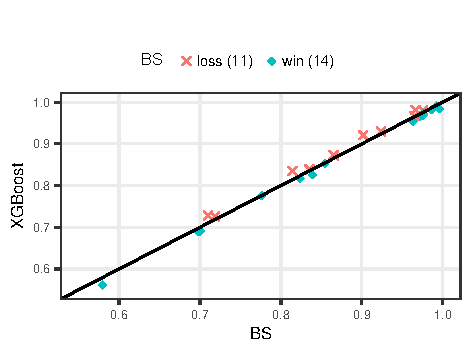
\includegraphics[width=.497\textwidth]{5_Guided_Search/fig/BS-Xgboost.pdf}
  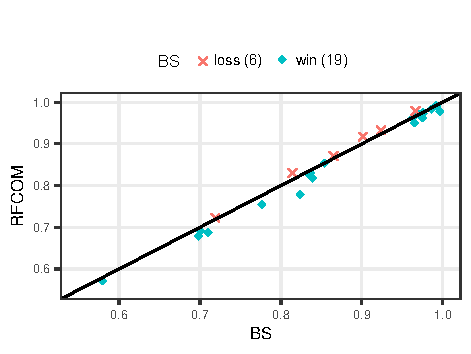
\includegraphics[width=.497\textwidth]{5_Guided_Search/fig/BS-RFCOM.pdf}\\
  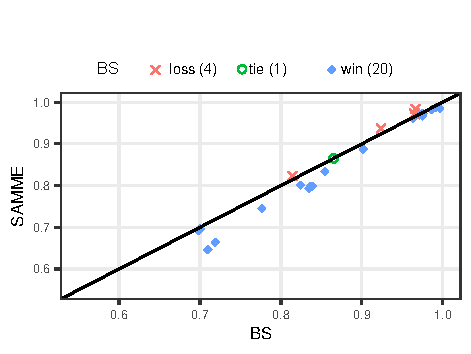
\includegraphics[width=.497\textwidth]{5_Guided_Search/fig/BS-SAMME.pdf}
  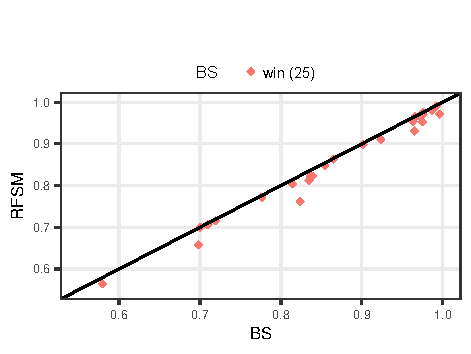
\includegraphics[width=.497\textwidth]{5_Guided_Search/fig/BS-RFSM.pdf}\\
  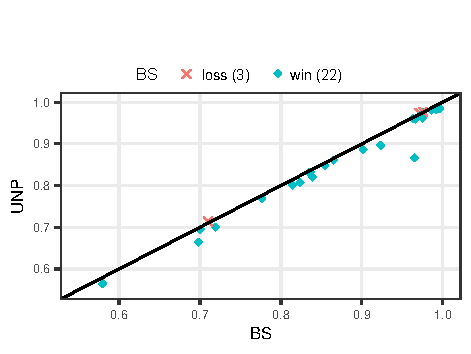
\includegraphics[width=.497\textwidth]{5_Guided_Search/fig/BS-UNP.pdf}
\end{center}
\caption{The performance of the proposed method against the defined ensembles NRD-NSE and RD-NSE.}
\label{BS-scatter}
\end{figure*}




\begin{figure*}[!ht]
\begin{center}\scriptsize
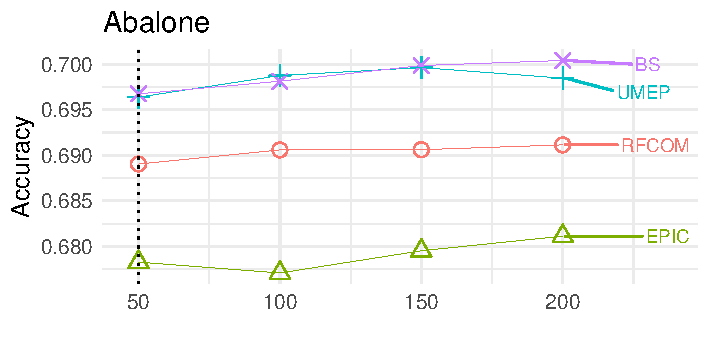
\includegraphics[width=.494\textwidth]{5_Guided_Search/fig/S-ENS-Abalone.pdf}
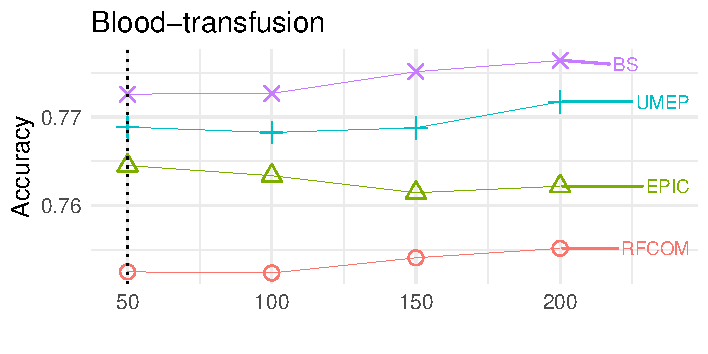
\includegraphics[width=.494\textwidth]{5_Guided_Search/fig/S-ENS-Blood-transfusion.pdf}\\
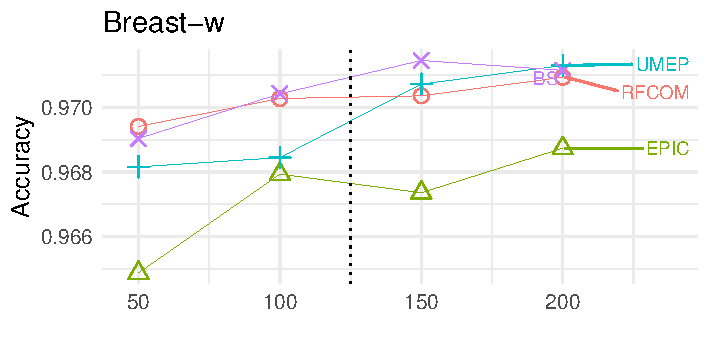
\includegraphics[width=.494\textwidth]{5_Guided_Search/fig/S-ENS-Breast-w.pdf} 
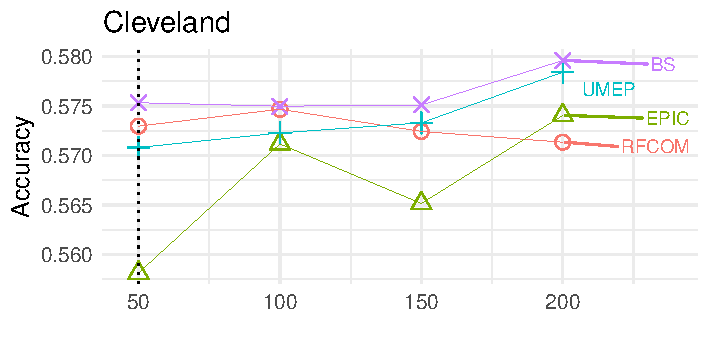
\includegraphics[width=.494\textwidth]{5_Guided_Search/fig/S-ENS-Cleveland.pdf}\\
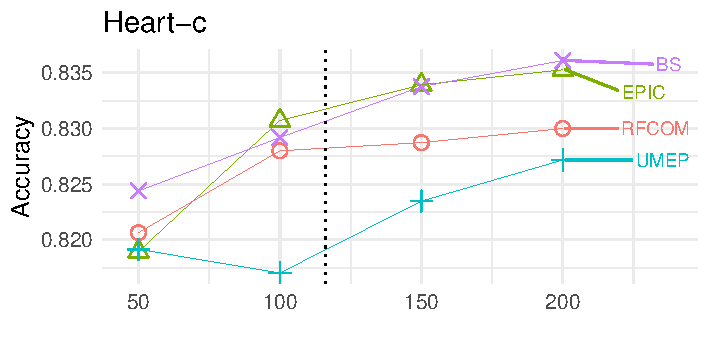
\includegraphics[width=.494\textwidth]{5_Guided_Search/fig/S-ENS-Heart-c.pdf}
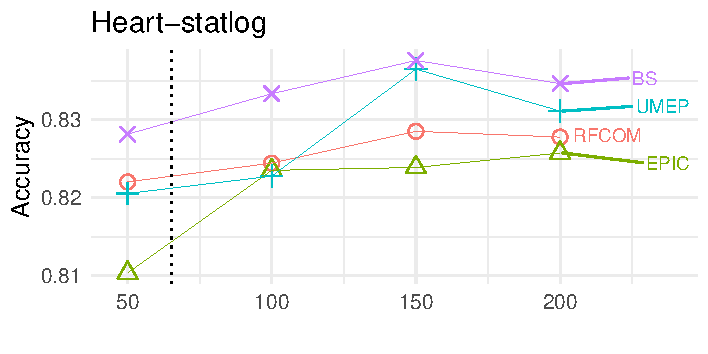
\includegraphics[width=.494\textwidth]{5_Guided_Search/fig/S-ENS-Heart-statlog.pdf}\\
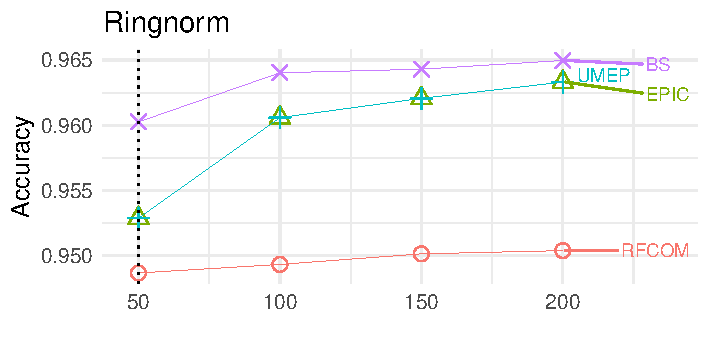
\includegraphics[width=.494\textwidth]{5_Guided_Search/fig/S-ENS-Ringnorm.pdf}
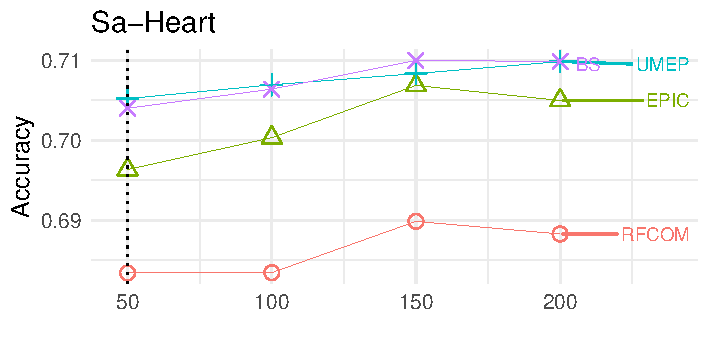
\includegraphics[width=.494\textwidth]{5_Guided_Search/fig/S-ENS-Sa-Heart.pdf}\\
\includegraphics[width=.495\textwidth]{5_Guided_Search/fig/S-ENS-Twonorm.pdf}
\includegraphics[width=.495\textwidth]{5_Guided_Search/fig/S-ENS-Wdbc.pdf}\\
\end{center}
\caption{The performance of ensemble pruning via guided search, a comparison with RFCOM, EPIC, and UMEP.}
\label{ch5:comparison.nonreduced}
\end{figure*}



It is interesting to analyze the performance of ensemble pruning via guided search for different ensemble sizes. This is important to check if its performance is consistent and not obtained due to randomness. Random Forest which is trained from whole training data, RFCOM, will be the baseline to compare against.  Figure \ref{ch5:comparison.nonreduced} shows the average accuracy of the pruned ensemble by (BS, UMEP, EPIC) and the unpruned one by RFCOM. Each point, in the figure, represents an average of 100 runs, and a percentage of $P=20\%$ is determined in advance to control the subensemble size. From Fig. \ref{ch5:comparison.nonreduced}, the behavior of BS dominates RFCOM according to both the accuracy and the ensemble size. Furthermore, the performance of BS over RFCOM can be reached, even, by pruning a low-size ensemble, the vertical dashed-line, regardless of what the size of RFCOM is. This shows how the proposed method can be an alternative to large-size ensembles, and a lot of computational resources could be saved by not overproducing models. However, this property could be different based on the classification task. We observe from Fig. \ref{ch5:comparison.nonreduced}, when EPIC and UMEP are ensembled together, via guided search, the subensemble realized a higher accuracy that was unreachable before. The statistical analysis will be discussed in Section \ref{statistical} to determine whether there is a significant improvement or not.







\subsection{Statistical Analysis}\label{statistical}
 To show if there is a significant improvement or not, Wilcoxon Signed Ranks Test \cite{wilcoxon1945} for pairwise comparison has been used. Table \ref{wilcoxontable} shows Wilcoxon Test \cite{wilcoxon1945} for the averages of the subensemble accuracy and subensemble size. The analysis from this table is as follows:
\begin{itemize}[nosep]
    \item[-] From the upper two parts (NRD-NSE, RD-NSE) which is a matrix 5 $\times$ 5: RFCOM significantly outperforms SAMME and RFSM by 90\% and 95\%, respectively. In addition, XGBoost is the best ensemble to learn from complete training data.
    \item[-] The proposed ensemble without pruning, UNP, is competitive with SAMME and RFCOM.
    
    \item[-] All RD-SE are significantly better than UNP in terms of accuracy and ensemble size, except FS and GA are only significantly better in terms of size. This proves the limitation of the proposed ensemble without pruning. 
    \item[-] HC and SA are comparable with UMEP, MDEP, and RFCOM in terms of accuracy, while HC and SA are significantly better in terms of subensemble size.
    \item[-] MDEP is comparable with RFCOM and UMEP in terms of accuracy. While it is better than RFCOM in terms of the ensemble size.
   
    \item[-] All RD-SE except FS and GA are comparable with XGBoost in terms of accuracy, while all RD-SE significantly outperform XGBoost in terms of ensemble size.  
    
     \item[-] BS is the only selection strategy under the proposed method that scores many ($\blacktriangle$). While it significantly outperforms the recent MDEP by 90\%.
     
    \item[-] In general, the lower part of Table \ref{wilcoxontable}, RD-SE,  includes subensembles with many ($\blacktriangle$) and many (\textbullet) where we have more flexibility to choose, according to the rigor of prediction and the computational resources.   
\end{itemize}

\vspace*{.3cm}
       

\begin{table*}[!ht]
\centering\scriptsize
\caption{Summary of the Wilcoxon test. Shape denotes the measure used, accuracy ($\blacktriangle$ $\triangle$) and size (\textbullet \textopenbullet). The filled shape ($\blacktriangle$ \textbullet) represents if the method in the row outperforms the one in the column or vice versa for ($\triangle$ \textopenbullet). Upper diagonal of level significance $\alpha=0.9$, lower diagonal level of significance $\alpha=0.95$.}

\resizebox{\textwidth}{!}{\begin{tabular}{|c
|l|c|c|c|c|c|c|c|c|c|c|c|c|c|c|}
\hline
& &(1) &(2) &(3) &(4) &(5) &(6) &(7) &(8) &(9) &(10) &(11) &(12)& (13)& (14) \\
\hline
\multirow{3}{*}{ NRD-NSE} & XGBoost(1) & - -& $\blacktriangle$ & $\blacktriangle$ & $\blacktriangle$ & $\blacktriangle$ & \textopenbullet & \textopenbullet  &\textopenbullet & $\blacktriangle$ \textopenbullet  &  \textopenbullet& \textopenbullet & \textopenbullet& \textopenbullet & $\blacktriangle$ \textopenbullet  \\
\cline{2-16}
 & SAMME(2) & $\triangle$ &- -& $\triangle$ &  &  & $\triangle$ \textopenbullet& $\triangle$ \textopenbullet &$\triangle$ \textopenbullet & \textopenbullet & $\triangle$ \textopenbullet & $\triangle$ \textopenbullet & $\triangle$  \textopenbullet& $\triangle$ \textopenbullet &  \textopenbullet \\
\cline{2-16}
&RFCOM (3)& $\triangle$ &  &- -& $\blacktriangle$ &  & \textopenbullet & $\triangle$ \textopenbullet &  \textopenbullet & $\blacktriangle$ \textopenbullet& $\triangle$\textopenbullet &  \textopenbullet &\textopenbullet  & \textopenbullet & \textopenbullet \\
\hline
\multirow{2}{*}{RD-NSE} &RFSM (4)&$\triangle$ &  & $\triangle$ &- -&  & $\triangle$ \textopenbullet & $\triangle$ \textopenbullet & $\triangle$ \textopenbullet & $\blacktriangle$ \textopenbullet & $\triangle$ \textopenbullet & $\triangle$ \textopenbullet & $\triangle$ \textopenbullet & $\triangle$ \textopenbullet & \textopenbullet  \\
\cline{2-16}
&UNP (5)&$\triangle$ &  &  &  &- -& $\triangle$ \textopenbullet & $\triangle$ \textopenbullet &$\triangle$ \textopenbullet &\textopenbullet & $\triangle$ \textopenbullet & $\triangle$ \textopenbullet  & $\triangle$ \textopenbullet & $\triangle$ \textopenbullet &  \textopenbullet \\
\hline
\multirow{8}{*}{RD-SE} &EPIC (6)& \textbullet& $\blacktriangle$\textbullet & \textbullet & $\blacktriangle$ \textbullet & $\blacktriangle$ \textbullet &- -& $\triangle$ &$\triangle$ &$\blacktriangle$ \textopenbullet & $\triangle$ \textbullet & $\triangle$ \textopenbullet & \textopenbullet & \textopenbullet & $\blacktriangle$ \textopenbullet \\
\cline{2-16}
&UMEP (7)&\textbullet & $\blacktriangle$ \textbullet & \textbullet  & $\blacktriangle$ \textbullet & $\blacktriangle$ \textbullet &$\blacktriangle$  &- -&  & $\blacktriangle$ \textopenbullet & $\triangle$ \textbullet &\textopenbullet  & \textopenbullet & $\blacktriangle$ \textopenbullet & $\blacktriangle$ \textopenbullet \\
\cline{2-16}
& MDEP(8) &\textbullet  & $\blacktriangle$\textbullet&  \textbullet&$\blacktriangle$ \textbullet  &$\blacktriangle$ \textbullet&$\blacktriangle$  &   &- -&$\blacktriangle$ \textopenbullet &$\triangle$  \textbullet& \textopenbullet & \textopenbullet & \textopenbullet  &$\blacktriangle$ \textopenbullet   \\
\cline{2-16}
&FS (9)& $\triangle$ \textbullet & \textbullet & $\triangle$ \textbullet & $\triangle$ \textbullet  & \textbullet  & $\triangle$ \textbullet & $\triangle$ \textbullet& $\triangle$ \textbullet &- -& $\triangle$ \textbullet & $\triangle$ \textbullet & $\triangle$ \textbullet & $\triangle$ \textbullet & $\triangle$ \textbullet \\
\cline{2-16}
&BS (10)& \textbullet& $\blacktriangle$ \textbullet & $\blacktriangle$ \textbullet & $\blacktriangle$ \textbullet & $\blacktriangle$ \textbullet & $\blacktriangle$ \textopenbullet& $\blacktriangle$ \textopenbullet & \textopenbullet & $\blacktriangle$ \textopenbullet &- -& $\blacktriangle$ \textopenbullet & $\blacktriangle$ \textopenbullet & $\blacktriangle$ \textopenbullet & $\blacktriangle$ \textopenbullet \\
\cline{2-16}
&HC (11)& \textbullet& $\blacktriangle$ \textbullet & \textbullet & $\blacktriangle$ \textbullet & $\blacktriangle$ \textbullet &$\blacktriangle$ \textbullet  & \textbullet &\textbullet & $\blacktriangle$ \textopenbullet & $\triangle$ \textbullet &- -&  & $\blacktriangle$ \textopenbullet & $\blacktriangle$ \textopenbullet \\
\cline{2-16}
&SA (12) & \textbullet& $\blacktriangle$ \textbullet & \textbullet & $\blacktriangle$ \textbullet & $\blacktriangle$ \textbullet & \textbullet  & \textbullet & \textbullet & $\blacktriangle$ \textopenbullet & $\triangle$ \textbullet&  &- -& $\blacktriangle$ \textopenbullet& $\blacktriangle$ \textopenbullet \\
\cline{2-16}
&BGWO (13) & \textbullet& $\blacktriangle$ \textbullet &  \textbullet & $\blacktriangle$ \textbullet & $\blacktriangle$ \textbullet& \textbullet  & $\triangle$ \textbullet &  \textbullet &$\blacktriangle$ \textopenbullet & $\triangle$ \textbullet& $\triangle$ \textbullet  &  \textbullet &- -& $\blacktriangle$ \textopenbullet\\
\cline{2-16}
&GA (14) & $\triangle$ \textbullet& \textbullet & \textbullet & \textbullet &  \textbullet & $\triangle$ \textbullet& $\triangle$ \textbullet &$\triangle$ \textbullet & $\blacktriangle$\textopenbullet & $\triangle$  \textbullet& $\triangle$ \textbullet  & $\triangle$ \textbullet& $\triangle$ \textbullet&- -\\
\hline
\end{tabular}}
\label{wilcoxontable}
\end{table*}



\afterpage{
\begin{landscape}
\begin{table}[!ht]
        \centering \scriptsize
\caption{Average accuracy and standard deviation of the proposed method with and without instance selection, ensemble size $T= 200$, $P$=20\%. The best value is in bold, while the second best is underlined.}
\label{wIS-complete-table}
\renewcommand{\arraystretch}{1.3}
\begin{adjustbox}{max width=1.5\textwidth} \begin{tabular}{llccccccccccccccc}
  \hline
   & & \multicolumn{5}{c}{Without Instance Selection}&\multicolumn{5}{c}{Instance Selection (Proposed)}\\
 \cmidrule(lr){3-7} \cmidrule(lr){8-12} 
 \#&  Dataset &  wIS-UNP & wIS-EPIC & wIS-UMEP & wIS-MDEP & \multicolumn{1}{c}{wIS-BS} & \multicolumn{1}{c}{UNP} & \multicolumn{1}{c}{EPIC} & \multicolumn{1}{c}{UMEP} &
 \multicolumn{1}{c}{MDEP} &
 \multicolumn{1}{c}{BS} \\ 
\hline
$D_1$ & Abalone &  \textbf{70.41$\pm$1.02}  & 69.31 $\pm$ 1.00  & 69.56 $\pm$ 1.14  & 69.48 $\pm$ 1.08  & 69.47 $\pm$ 1.08  &  69.52 $\pm$ 0.64 & 68.11 $\pm$ 1.80 & 69.85 $\pm$ 1.00 & 69.96 $\pm$ 1.12   & \underline{70.04 $\pm$ 1.14}\\ 

  $D_2$ & Australian &  87.00$\pm$ 3.10  & \textbf{87.18 $\pm$ 2.92}  & 86.89 $\pm$ 2.93  & 87.13 $\pm$ 2.91  & \underline{87.14 $\pm$ 2.88}  & 86.05 $\pm$ 2.46 & 85.47 $\pm$ 2.62 & 86.43 $\pm$ 2.65 & 86.25 $\pm$ 2.80 &  86.50 $\pm$ 2.60 \\ 
  
  $D_3$ & Blood-transfusion &  \underline{77.24$\pm$ 1.38}  & 77.20 $\pm$ 2.16  & 76.92 $\pm$ 2.14 & 77.19 $\pm$ 2.09   & 77.03 $\pm$ 2.10 &  76.90 $\pm$ 1.45 & 76.22 $\pm$ 3.65 & 77.17 $\pm$ 2.08 &77.22 $\pm$ 2.08  & \textbf{77.64 $\pm$ 2.22}\\ 
  
  $D_4$ & Breast-w &  \underline{97.25$\pm$ 1.43} & 96.96 $\pm$ 1.56 & 97.17 $\pm$ 1.41 & 97.19 $\pm$ 1.48	  & 97.20 $\pm$ 1.47
 &   \textbf{97.42 $\pm$ 1.17}  & 96.87 $\pm$ 1.30 & 97.13 $\pm$ 1.25 &97.13 $\pm$ 1.31   & 97.12 $\pm$ 1.23  \\ 
  
  $D_5$ & Cleveland &  57.47$\pm$ 3.04  & 57.58 $\pm$ 3.46 & 57.43 $\pm$ 3.08  & 57.60 $\pm$ 3.02  & 57.40 $\pm$ 3.57  &  56.50 $\pm$ 2.88 &57.41 $\pm$ 4.27 & \underline{57.84 $\pm$ 3.12} & 57.56 $\pm$ 3.10 & \textbf{57.96 $\pm$ 3.66} \\ 
  
  $D_6$ & Dermatology &  97.75$\pm$ 1.45  & 97.86 $\pm$ 1.58  & \textbf{97.93 $\pm$ 1.47}  & \textbf{97.93 $\pm$  1.49}	 & \underline{97.92 $\pm$ 1.47}
  &  97.46 $\pm$ 1.65 & 97.32 $\pm$ 1.89 & 97.56 $\pm$ 1.62 & 97.63 $\pm$ 1.65  & 97.53 $\pm$ 1.72 \\ 
  
  $D_7$ & Diabetic &  \textbf{71.08$\pm$ 2.79}  & 68.64 $\pm$ 2.46  & 68.68 $\pm$ 2.52  & 68.71 $\pm$  2.33  & 68.59 $\pm$ 2.44  &  66.38 $\pm$ 2.94 & 69.63 $\pm$ 2.75  & 70.26 $\pm$ 3.20 &\underline{70.49 $\pm$ 3.00}& 69.81 $\pm$ 3.10 \\ 
  
  $D_8$ & Heart-c &  \textbf{84.02 $\pm$ 4.38} & 82.65 $\pm$ 4.28 & 82.64 $\pm$ 4.19  & 82.60 $\pm$ 4.17  & 82.97 $\pm$ 4.05 &  83.22 $\pm$ 4.49 & 83.53 $\pm$ 4.25 & 82.72 $\pm$ 4.58 & 83.12 $\pm$ 4.33 & \underline{83.61 $\pm$ 4.26}\\ 
  
  $D_9$ & Heart-statlog &  \textbf{83.98$\pm$ 4.09} & 82.69 $\pm$ 4.13 & 82.50 $\pm$ 4.45 & 82.83 $\pm$ 4.28  & 82.72 $\pm$ 4.26 & 83.07 $\pm$ 4.71 & 82.57 $\pm$ 4.45 & 83.11 $\pm$ 4.07 &\underline{83.70 $\pm$ 4.26}&  83.46 $\pm$ 4.27 \\ 
  
  $D_{10}$ & Ionosphere &  93.32$\pm$ 2.98  & 93.85 $\pm$ 2.77 &  \textbf{93.96 $\pm$ 2.67}  & \underline{93.93 $\pm$ 2.79}   & \underline{93.93 $\pm$ 2.76} & 89.67 $\pm$ 2.98 & 92.41 $\pm$ 2.61  & 91.93 $\pm$ 2.89 &92.49 $\pm$ 2.74&  92.34 $\pm$ 2.75 \\ 
  
  $D_{11}$ & Led24 &  \underline{71.99 $\pm$ 1.61}  & 70.37 $\pm$ 1.78  & \textbf{72.04 $\pm$ 1.47} & 69.84 $\pm$ 2.67  & 67.84 $\pm$ 2.82 &  70.02 $\pm$ 1.76 & 71.75 $\pm$ 1.46 & 71.78 $\pm$ 1.45 & 68.66 $\pm$ 3.79&  71.89 $\pm$ 1.45 \\ 
  
  $D_{12}$ & Mammographic &  82.85 $\pm$ 2.67  & 83.32 $\pm$ 2.63	  & 83.57 $\pm$ 2.13	 & 83.66 $\pm$ 2.21	& 83.84 $\pm$ 2.34
 & 82.06 $\pm$ 2.51 & 83.37 $\pm$ 2.64 & \underline{84.00 $\pm$ 2.32} &\textbf{84.05 $\pm$ 2.27}& 83.89 $\pm$ 2.36 \\ 
  
  $D_{13}$ & Mfeat-fourier &  82.81 $\pm$ 1.44  & 83.24 $\pm$ 1.32  & 83.32 $\pm$ 1.40 & \textbf{83.48 $\pm$ 1.42}  & \underline{83.38 $\pm$ 1.48}  & 80.14 $\pm$ 1.50 & 80.89 $\pm$ 1.65 & 81.34 $\pm$ 1.56 &81.12 $\pm$ 1.63 &  81.41 $\pm$ 1.62 \\ 
  
  $D_{14}$ & Mfeat-karh &  \textbf{96.80$\pm$ 0.86} & 95.82 $\pm$ 0.83	  & 95.84 $\pm$ 0.86 & 95.98 $\pm$ 0.89  & 95.96 $\pm$ 0.86 & 96.13 $\pm$ 0.88 & 96.19 $\pm$ 0.86 & 96.27 $\pm$ 0.85 &96.28 $\pm$ 0.96 &\underline{96.31 $\pm$ 0.89} \\ 
  
  $D_{15}$ & Mfeat-zernike &  80.06$\pm$ 1.22  & 78.15 $\pm$ 1.48  & 78.83 $\pm$ 1.35 & 79.37 $\pm$ 1.39  & 78.89 $\pm$ 1.37  &  80.72 $\pm$ 1.24 & 82.19 $\pm$ 1.52 & \textbf{82.48 $\pm$ 1.44} &82.20 $\pm$ 1.41 &\underline{ 82.38 $\pm$ 1.39} \\ 
  
  $D_{16}$ & Optdigits &  98.29$\pm$ 0.35 & 98.79 $\pm$ 0.33 & \underline{98.80 $\pm$ 0.32}  & \underline{98.80 $\pm$ 0.32}  & \textbf{98.81 $\pm$ 0.32}  &  98.09 $\pm$ 0.38 & 98.61 $\pm$ 0.31 & 98.60 $\pm$ 0.31 &98.59 $\pm$ 0.30 & 98.61 $\pm$ 0.32 \\ 
  
  $D_{17}$ & Penbased &  98.31$\pm$ 0.27 & \textbf{99.32 $\pm$ 0.16}	 & 99.30 $\pm$ 0.17 & 99.29 $\pm$  0.17 & \underline{99.31 $\pm$ 0.16}  &  98.22 $\pm$ 0.27 & 99.21 $\pm$ 0.16 & 99.19 $\pm$ 0.17 &99.10 $\pm$ 0.69 &  99.20 $\pm$ 0.16  \\ 
  
  $D_{18}$ & Ringnorm &  \textbf{96.66$\pm$ 0.46}  & 96.62 $\pm$ 0.47 & 96.64 $\pm$ 0.49 & 96.64 $\pm$ 0.49  & \underline{96.65 $\pm$ 0.47}  &  86.69 $\pm$ 1.15 & 96.33 $\pm$ 0.51 & 96.33 $\pm$ 0.51 & 96.37 $\pm$ 0.49 &  96.50 $\pm$ 0.48 \\ 
  
  $D_{19}$ & Sa-heart &  71.23$\pm$ 3.38 & 69.06 $\pm$ 3.56	 & 69.13 $\pm$ 3.56 & 69.44 $\pm$ 3.39  & 69.35 $\pm$ 3.19
 & \textbf{71.41 $\pm$ 3.77} & 70.50 $\pm$ 4.30 & 70.98 $\pm$ 3.86 & \underline{71.25 $\pm$ 3.65} & 70.98 $\pm$ 4.06 \\ 
  
  $D_{20}$ & Satimage &  89.45$\pm$ 0.74  & 91.33 $\pm$ 0.73  & 91.33 $\pm$ 0.73 & \underline{91.34 $\pm$ 0.72}   & \textbf{91.39 $\pm$ 0.75}
 & 88.70 $\pm$ 0.78 & 90.17 $\pm$ 0.75 & 90.05 $\pm$ 0.77 & 89.81 $\pm$ 1.39 &  90.16 $\pm$ 0.72  \\
 
  $D_{21}$ & Segment &  96.87$\pm$ 0.89	 & \textbf{98.05 $\pm$ 0.68}  & 98.00 $\pm$ 0.68 & 98.01 $\pm$ 0.69 & \underline{98.03 $\pm$ 0.65}  &  95.94 $\pm$ 0.90 & 96.61 $\pm$ 0.77 & 96.54 $\pm$ 0.74 & 96.51 $\pm$ 0.87 & 96.61 $\pm$ 0.77  \\ 
  
  $D_{22}$ & Texture &  98.80$\pm$ 0.33	  & \textbf{99.71 $\pm$ 0.17} & \textbf{99.71 $\pm$ 0.17} & \textbf{99.71 $\pm$ 0.17}  & \textbf{99.71 $\pm$ 0.17} &  98.40 $\pm$ 0.35 & \underline{99.63 $\pm$ 0.19} & \underline{99.63 $\pm$ 0.19} &\underline{99.63 $\pm$ 0.16} & \underline{99.63 $\pm$ 0.18} \\ 
  
  $D_{23}$ & Twonorm &  \textbf{97.69$\pm$ 0.36}	  & 96.61 $\pm$ 0.45 & 96.62 $\pm$ 0.44  & 96.62 $\pm$ 0.44   & 96.68 $\pm$  0.41 & \textbf{ 97.69 $\pm$ 0.37}& 97.38 $\pm$ 0.39 & 97.46 $\pm$ 0.38 &97.47 $\pm$ 0.42 &\underline{ 97.55 $\pm$ 0.35} \\ 
  
  $D_{24}$ & Waveform &  \textbf{85.66 $\pm$ 1.04}	 & 84.42 $\pm$ 1.11	 & 84.39 $\pm$ 1.15  & 84.40 $\pm$ 1.17  & 84.46 $\pm$ 1.11
  &  84.87 $\pm$ 1.16 & 84.59 $\pm$ 1.00 & 85.41 $\pm$ 0.95 &85.34 $\pm$ 1.07 & \underline{85.42 $\pm$ 0.93} \\ 
  
  $D_{25}$ & Wdbc &  96.81$\pm$ 1.44  & \underline{97.57 $\pm$ 1.21}  & 97.46 $\pm$ 1.29  & 97.56 $\pm$ 1.22  & \textbf{97.66 $\pm$ 1.16} &  96.17 $\pm$ 1.85 & 97.52 $\pm$ 1.46 & 97.48 $\pm$ 1.63 &97.34 $\pm$ 1.58 & 97.49 $\pm$ 1.56 \\ 
  
   \hline
  \multicolumn{2}{c}{\textbf{AR-Friedman}}& \multicolumn{1}{c}{\textbf{4.3}} &\multicolumn{1}{c}{5.76}&\multicolumn{1}{c}{5.6} &\multicolumn{1}{c} {4.84} &\multicolumn{1}{c}{4.88} &\multicolumn{1}{c} {7.54} & \multicolumn{1}{c}{6.84}& \multicolumn{1}{c}{5.44} &\multicolumn{1}{c}{5.4} &\multicolumn{1}{c}{\underline{4.4}}  \\ 
\hline
\end{tabular}
\end{adjustbox}
\end{table}
\end{landscape}
}


\subsection{Validation of the Methodology}
We have shown the superiority of the proposed ensemble in the previous sections. However, it is necessary to validate its components (instance selection, proposed ensemble, and guided search-based pruning). Thus, we performed additional experiments to validate our method.  

\textit{The effect of instance selection to the constructed ensemble}, we compared the obtained results without instance selection (wIS) and with instance selection (proposed). Table \ref{wIS-complete-table} shows the complete results of the 25 datasets. The worst average rank via Friedman Test \cite{demsar2006} is scored by UNP. Hence, coupling instance selection with the unpruned proposed ensemble has a limited accuracy in comparison with wIS-UNP. This means that IS contributed to form simpler, less space complexity, ensembles rather than more accurate ensembles. Table \ref{wIS-wilcoxon-table} shows the Wilcoxon Test \cite{wilcoxon1945} for the results from Table \ref{wIS-complete-table}. The results confirm that the proposed ensemble without pruning, UNP, is not effective. However, it is comparable with ensembles that are trained from whole training data, RFCOM and SAMME.

\textit{The validation of the proposed ensemble}, we show how the proposed ensemble, Section \ref{proposed.mcs}, is effective. Table \ref{wIS-wilcoxon-table} confirms that wIS-UNP which uses the same amount of training data is significantly better than SAMME and RFCOM at a 95\% confidence level. Furthermore, there is no ensemble, among the thirteen models, that is significantly higher than wIS-UNP.   


\textit{The validation of guided search-based pruning}, we prove how guided search is more effective whether an instance selection is applied or not. From Table \ref{wIS-wilcoxon-table}, when instance selection is performed, BS shows a significant difference at a 95\% confidence level better than EPIC and UMEP. In addition, MDEP is significantly worse than BS at a 90\% confidence level. Moreover, BS is able to compensate for the error of UNP, confirmed by the significant difference between BS and RFCOM. Without applying instance selection, wIS-BS is still outperforming wIS-EPIC and wIS-UMEP at a 95\% confidence level. This shows the limited performance of the existing pruning methods in comparison with the proposed guided search-based pruning. 


As a summary, with the experiments of this section. We have separately validated the different parts of our method, showing their usefulness. We proved that simpler and better ensembles could be properly designed when all the parts are used together.  
\vspace*{.3cm}

\begin{table}[!ht]
\centering\scriptsize
\caption{Summary of the Wilcoxon test. $\blacktriangle$ = the method in the row improves the method of the column. $\triangle$ = the method in the column improves the method of the row. Upper diagonal of level significance $\alpha=0.9$, Lower diagonal level of significance $\alpha=0.95$}
\label{wIS-wilcoxon-table}
{\begin{tabular}{
|l|c|c|c|c|c|c|c|c|c|c|c|c|c|}
\hline
&(1) &(2) &(3) &(4) &(5) &(6) &(7) &(8) &(9) &(10) &(11) &(12) &(13) \\
\hline
XGBoost (1)& -& $\blacktriangle$ & $\blacktriangle$ &  &  &  &  &  & $\blacktriangle$ &  &  &  &  \\
\hline
SAMME (2)& $\triangle$ & -& $\triangle$ & $\triangle$ & $\triangle$ & $\triangle$ & $\triangle$ & $\triangle$ &  & $\triangle$ & $\triangle$ & $\triangle$ & $\triangle$ \\
\hline
RFCOM (3)& $\triangle$ &  & -& $\triangle$ & $\triangle$ & $\triangle$ & $\triangle$ & $\triangle$ &  &  & $\triangle$ &  & $\triangle$ \\
\hline
wIS-UNP (4)&  & $\blacktriangle$ & $\blacktriangle$ & -&  &  &  &  & $\blacktriangle$ & $\blacktriangle$ &  &  &  \\
\hline
wIS-EPIC (5)&  & $\blacktriangle$ &  &  & -&  & $\triangle$ & $\triangle$ & $\blacktriangle$ &  &  &  &  \\
\hline
wIS-UMEP (6)&  & $\blacktriangle$ & $\blacktriangle$ &  &  & -& $\triangle$ & $\triangle$ & $\blacktriangle$ &  &  &  &  \\
\hline
wIS-MDEP (7)&  & $\blacktriangle$ & $\blacktriangle$ &  & $\blacktriangle$ & $\blacktriangle$ & -&  & $\blacktriangle$ &  &  &  &  \\
\hline
wIS-BS (8)&  & $\blacktriangle$ & $\blacktriangle$ &  & $\blacktriangle$ & $\blacktriangle$ &  & -& $\blacktriangle$ &  &  &  &  \\
\hline
UNP (9)& $\triangle$ &  &  & $\triangle$ &$\triangle$ & $\triangle$ & $\triangle$ &  & -& $\triangle$ & $\triangle$ & $\triangle$ & $\triangle$ \\
\hline
EPIC (10)&  & $\blacktriangle$ &  &  &  &  &  &  & $\blacktriangle$ & -& $\triangle$ & $\triangle$ & $\triangle$ \\
\hline
UMEP (11)&  & $\blacktriangle$ &  &  &  &  &  &  & $\blacktriangle$ & $\blacktriangle$ & -&  & $\triangle$ \\
\hline
MDEP (12)&  & $\blacktriangle$ &  &  &  &  &  &  & $\blacktriangle$ & $\blacktriangle$ &  & -& $\triangle$ \\
\hline
BS (13)&  & $\blacktriangle$ & $\blacktriangle$ &  &  &  &  &  & $\blacktriangle$ & $\blacktriangle$ & $\blacktriangle$ &  & -\\
\hline
\end{tabular}}
\end{table}





\subsection{Advantages of the proposed method}

Among the advantages of the proposed method are: (1) The instance selection method is applied only once from the whole training data. (2) The individual models are independent, and the generation step could be accelerated by a parallel implementation. (3) The reduced data helps to generate less complex models with a fast prediction time. (4) The guided search preserves promising search areas to identify a subensemble properly. (5) The proposed methodology proved its capability to maximize learning from the reduced data. Regarding that, it can be used to improve the precision of IS method. (6) The ease of implementation with wide flexibility to apply different IS methods and different classifier types.



\subsection{Time Complexity} \label{complex}
The classification speed as determined in \citep{martinez2009} mainly depends on (1) the ensemble size and (2) the complexity of individual classifiers. While Table \ref{complecity} summarize the time complexity of the applied ensemble pruning methods. For GA \& BGWO, ($\hat P$) represents population size, and ($E$) represents the number of epochs. While $\hat{T}$ denotes the size of the preselected classifiers, \textit{New subset in Fig. \ref{topology}}, that is formed by both EPIC \& UMEP.
\vspace*{.3cm}

\begin{table}[!ht]
\centering
 \caption{Time complexity of ensemble selection}
\label{complecity}
\renewcommand{\arraystretch}{1}
\begin{adjustbox}{max width=1\textwidth}
\begin{tabular}{l|l}
\hline
Ensemble selection & Time complexity\\ \hline
MDEP & $\mathcal{O}( T \cdot  \log{T})$\\
UMEP & $\mathcal{O}(T \cdot N) \rightarrow$  \circled{1}\\
EPIC & $\mathcal{O}( T \cdot\log{T}) \rightarrow$ \circled{2}\\
FS \& BS   &\circled{1}+\circled{2}+ $\mathcal{O}({\hat{T}}^3)$\\
HC - SA & \circled{1}+\circled{2}+ $\mathcal{O}( \hat{T} \cdot N \cdot M)$ \\
GA - BGWO & \circled{1}+\circled{2}+ $\mathcal{O}(E \cdot \hat P \cdot \hat{T} \cdot N \cdot M)$\\
\hline
\end{tabular}
\end{adjustbox}
\end{table}
  
%%%%%%%%%%%%%%%%%%%%%%%%%%%%%%%%%%%%%%%%%%%%%%%
%
%   Conclusions
%
%%%%%%%%%%%%%%%%%%%%%%%%%%%%%%%%%%%%%%%%%%%%%%%
\subsection{Exploration of the Research Questions} 

In this part, we determine whether the research questions of the second objective are answered or not. 

\textit{\textbf{($\pmb{Q_3}$)} The effect of combining multiple pruning metrics} is so promising to go beyond, in terms of accuracy, what can be achieved from each metric alone. This has been confirmed by the outperformance of BS over both EPIC and UMEP in many datasets. In addition, the proposed method significantly outperforms MDEP by 90\% without any dependence on assuming parameters in advance. Furthermore, new promising solutions can be reached in terms of both subensemble size and subensemble accuracy, i.e. (HC, SA, and BGWO). 

\textit{\textbf{($\pmb{Q_4}$)} The effect of downsizing data and downsizing the number of classifiers simultaneously} has been confirmed experimentally and statistically. The RD-NSE represented by RFSM and UNP have a limited accuracy while depending on the whole ensemble members. In contrast, RD-SE represented by the lower part of Table \ref{wilcoxontable} has many ($\blacktriangle$) and many (\textbullet) where we have more flexibility to choose among them, according to the rigor of prediction and the ensemble size. Furthermore, the best investigated RD-SE represented by BS proved its significant superiority over state-of-art ensembles that are trained from non reduced data. 

\section{Conclusions}
\label{ch5_conclusions}
In this chapter,  we have proposed a new method to alleviate the drawbacks while building and pruning an ensemble of classifiers. The objective was to generate less complex and small-size ensembles. Thus, a dual reduction on the data level and ensemble level has been considered. An instance selection method is applied to downsize the training set. After that, a bagging-like ensemble is proposed to train a set of classifiers from the reduced data. The advantage of this step is to form ensemble models quickly, especially when we generate a large number of models. In addition, the complexity of ensemble members will be reduced. 

The ensemble accuracy and the ensemble size are so important and both of them can be improved through ensemble selection strategies. However, the pruning method could be biased by the selection criteria. Therefore, we have proposed a guided search that captures the properties of ensemble diversity and the individual's accuracy simultaneously. The proposed pruning strategy is capable to compensate for the limited accuracy of the unpruned ensemble. Furthermore, we showed, graphically, how the proposed method could be an alternative to large-size ensembles. The statistically significant difference is conducted by rank-based transformations to show the superiority of the proposed methodology. The second set of experiments were conducted to validate the connected components. Notably, the superiority of the system was endowed via guided search. Moreover, the proposed method was able to maximize the learning from the reduced data.


Regarding future research, the framework can be enhanced by applying different training set selection methods. In addition, multi-objective optimization will be applied to capture the conflict between the ordering-based ensemble pruning methods that have been discussed.  Furthermore, a weighted sum voting will be applied to fuse the pruned classifiers. 





% our_proposal
% % this file is called up by thesis.tex
% content in this file will be fed into the main document


% this file is called up by thesis.tex
% content in this file will be fed into the main document

%: ----------------------- introduction file header -----------------------


\begin{savequote}[50mm]
As long as I have a want, I have a reason for living. Satisfaction is death.  
\qauthor{George Bernard Shaw}
% The beginning is the most important part of the work.
% \qauthor{Plato}
\end{savequote}


\chapter{An Analysis of Heuristic Metrics for MCS Pruning}
\label{cha:6_our_proposal}

Including more classifiers in the classification task may provide more discriminating power with an equal or weighted contribution of each classifier to the final decision \cite{cao2018}. However, the increasing size of the ensemble hardly copes with the increasing demand to speed up the decision and to save computational resources. In bagging \cite{breiman1996}, an independent set of classifiers are generated in random order, then the final decision is adopted by a simple majority voting-based aggregation. While, it has been demonstrated that reordering the generated pool and selecting the first subset of classifiers impacts the ensemble size and the composite accuracy positively \cite{cao2018,martinez2004,martinez2009, guo2013, guo2018,lu2010}. The first subset of classifiers from the ordered list is expected to perform better than aggregating the whole list. 

It has been proved that the generalization performance of a subensemble reports superior results over the traditional combination approaches, such as majority voting of the whole ensemble \cite{martinez2009,zhou2002}.
Moreover, pruning down the redundant models reduces the memory burden \cite{diao2013}. Regarding that, MCS pruning is a proven mechanism to enhance the efficiency and elevate the efficacy of classification ensemble systems \cite{cao2018,martinez2009,guo2013, lu2010}. From the review of the different pruning strategies in chapter \ref{ch5_GUided_MCS_Pruning}, ordered-based pruning is a fast strategy with proven accuracy. Those strategies
have the following merits: (1)           return subsets that are close to optimal solution (\textit{Efficacy}) \cite{martinez2009}.
   (2)  easy adaptation to any given storage and computational restrictions \cite{cao2018,guo2018}.
    (3) the time complexity of those strategies is low, in comparison with exhaustive or optimization-based search methods (\textit{Efficiency}) \cite{martinez2009}.
 

The classifiers can be reordered via a greedy search, where the set of classifiers that are expected to perform better are aggregated first. Sequentially a new subset $S_u$ is constructed from $S_{u-1}$ by incorporating a single classifier from $L_{u-1}$; $S_{u}=S_{u-1}\cup \Psi_{k} \Big| \Psi_{k} \in L_{u-1}$, where $T= S_u \cup L_u$ and $u=\{1,2,3,\dots,T\}$. Such that the single classifier selection from $L_{u-1}$ is guided upon \textit{a heuristic metric} to optimize the augmented ensemble $S_u$. The number of iterations or subensemble size, $\hat{T}$, can be controlled in advance to meet the computational restrictions. Furthermore, some metrics were proposed to rank all the classifiers in one batch without the sequential search. While, the property of the base classifier, an individual's accuracy, is not effective to determine this rank \cite{martinez2004}. The generated ensemble needs to consider the hybrid between an individual's performance and an individual contribution to the ensemble diversity \cite{guo2018,lu2010}. Where it has been confirmed that the weakness of individuals can be compensated by the consensus of correct peers over different samples. 

Since the practical analysis of the power of greedy search methods in \cite{martinez2009}, many research efforts have been directed to propose new heuristic measures to guide the selection of subensemble  \cite{cao2018,guo2013,guo2018,lu2010}. Till now and related to our best knowledge, no work has considered the analysis of all those promising metrics together. This chapter fills that gap by comparing all these new techniques with the best performing techniques found in \cite{martinez2009}, and against other popular baseline metrics \cite{martinez2004,margineantu1997}.

In this chapter, we shed light on the importance of ordering-based ensemble pruning metrics. Reviewing and analyzing popular and recent metrics that work for bagging-based ensembles. We present a sophisticated analysis of how the pruning metrics can be affected by; the initial ensemble size ($T$), the required subensemble size ($\hat{T}$), the individual classifier type, and the binary or multiclass classification task.  In addition, this study can be considered as a secure methodology to elevate the performance of bagging-like ensembles. This analysis is promising due to the precision, prediction consistency, time-complexity, and space complexity of the investigated metrics to meet different computational restrictions. 


Finally, this chapter is organized as follows: In Section \ref{ch6_motivations}, we present the main motivations to conduct this research and our contributions. The heuristic metrics in detail are to be introduced in Section \ref{ch6_heuristic-met}. The experimental results and the statistical analysis are presented in Section \ref{sec:6_2_methodology}.  Finally, the conclusions are presented in Section \ref{ch6_Conclusion}.


  


\section{Motivations and Contributions} \label{ch6_motivations}

The contribution of this proposal can be highlighted in the following points:
\begin{enumerate}[nosep]
    \item Focusing on static ensemble selection as an active research topic in multiple classifier systems.
    \item Analyzing the effectiveness of different heuristic metrics to reorder the randomly bagging ensembles.
    \item Separate analysis of those metrics over binary and multiclass classification tasks.
    \item As far as we know, we are the first to group recent and efficient heuristic metrics for reordering bagging ensembles since they were analyzed by Martínez-Muñoz et al. \citep{martinez2009} in 2009.    
    
\end{enumerate}

\section{Heuristic Metrics} \label{ch6_heuristic-met}

The investigated metrics are based on modifying the order of the classifiers in the bagging algorithm with the selection of the first set in the queue. Those techniques comprise dissimilar heuristic measures as: ensemble diversity \cite{lu2010}, ensemble margin \cite{martinez2004,guo2013}, margin hybrid diversity \cite{guo2018}, discriminating classifiers \cite{cao2018}, ensemble error \cite{margineantu1997}, Complementariness of misclassification \cite{martinez2004}, and relative accuracy with minimum redundancy \cite{cao2018}. Table \ref{metrics} shows the heuristic metrics to be analyzed in this chapter over 30 datasets, divided into two parts as 15 binary datasets and 15 multiclass datasets.      
          
\begin{table}[!ht]
 \centering \scriptsize
 \caption{Heuristic metrics to guide the ordered bagging ensembles.}
\label{metrics}
\begin{tabular}{l|c|l|l|l}
\hline
Name & Section &Heuristic Measure & Year & Ref.\\ \hline
RE & \ref{ch6_RE} & Reduced Ensemble Error & 1997 & \cite{margineantu1997} \\
CC & \ref{ch6_CC} & Complementary of Misclassification & 2004 & \cite{martinez2004}\\
MDSQ  & \ref{ch6_MDSQ} & Supervised Ensemble Margin & 2009 & \cite{martinez2009}\\
EPIC & \ref{ch5_EPIC.div} &Diversity Contribution of Individuals & 2010 & \cite{lu2010}\\
UMEP & \ref{ch5_UMEP} &Unsupervised Ensemble Margin & 2013 & \cite{guo2013}\\
MDEP &\ref{ch5_MDEP} &Margin \& Diversity & 2018 & \cite{guo2018}\\
MRMR & \ref{ch6_MRMR} &Max. Relevance \&  Min. Redundancy & 2018 & \cite{cao2018}\\
DISC &\ref{ch6_DISC} &Discriminant Classifiers & 2018 & \cite{cao2018}\\
\hline
\end{tabular}
\end{table}     


\subsection{Reduce-Error Pruning} \label{ch6_RE}
Reduce error pruning (RE) was firstly proposed in \cite{margineantu1997}. The classifier with the highest (lowest) accuracy (error), as estimated on the pruning set $D_{pr}$, is stored in $S_1$ as the initial subset to be extended. The sequential addition of more classifiers, one at a time, is performed to get as much (less) accuracy (error) as possible. This heuristic incorporates into the subensemble the classifier $s_u$ as:  

\begin{equation}
\label{Reduced.err}
s_u=\mathop{\arg\max}\limits_{k} \mathop{\sum}\limits_{(\textbf{x}_i,y_i) \in D_{pr}} \left[\hat{\Psi}_{S_{u-1}\cup \Psi_k} (\textbf{x}_i) =y_i\right] 
\end{equation}

\noindent where the index $k \in L_{u-1}$ and $S_u=S_{u-1} \cup \{s_u\}$. That metric has been applied in many articles as a baseline for the comparison purpose \cite{cao2018,guo2013} with superior performance over the unpruned ensemble \cite{martinez2009}.


\subsection{Complementariness measure} \label{ch6_CC}

Complementariness measure (CC) was proposed in \cite{martinez2004} and it considers the complementariness between the incorporated models. The first subset, $S_1$, is initialized by selecting the classifier with the highest accuracy on $D_{pr}$. Then, the classifier to be nominated is the one with the highest prediction accuracy over the set of instances that are misclassified by $S_{u-1}$: 

\begin{equation}
\scalemath{0.95}{
\label{complementary.miss}
s_u=\mathop{\arg\max}\limits_{k} \mathop{\sum}\limits_{(\textbf{x}_i,y_i) \in D_{pr}} \left[\hat{\Psi}_{S_{u-1}} (\textbf{x}_i) \neq y_i  \wedge \Psi_{k}(\textbf{x}_i)=y_i\right] 
}
\end{equation}

\noindent where $k \in L_{u-1}$ and $S_u=S_{u-1} \cup \{s_u\}$. With this heuristic, the ensemble decision is expected to be shifted towards the correct classification. However, this metric concentrates only on the misclassified samples with no restriction to preserve the previous correct decisions.

\subsection{Supervised Ensemble Margin} \label{ch6_MDSQ}
Margin distance minimization (MDSQ) is introduced in \cite{martinez2004,martinez2009}, where the decision space of the individual members over the selection set, $D_{pr}$, is transformed into signature vectors. The signature vector of $\Psi_k$, $r^{(k)}$, is defined by an N-dimensional vector whose $i$th component is calculated as: 

\begin{equation}
\label{sign.vect}
r_{i}^{(k)}=2 \left[\Psi_{k}(\textbf{x}_i)=y_i\right]-1 \quad (\textbf{x}_i,y_i) \in D_{pr}
\end{equation}

 The quantity $r_{i}^{(k)}$ will be 1, if the $k$th classifier correctly classifies the $i$th example in $D_{pr}$, otherwise it will be -1. The ensemble signature vector, $\langle R \rangle$, is defined as the average sum of all $r^{(k)}$ as: 

\begin{equation}
\label{ens.sign}
\langle R \rangle=T^{-1} \mathop{\sum}\limits_{k=1}^{T} r^{(k)} 
\end{equation}

The subensemble whose average signature vector $\langle R \rangle$ is in the first quadrant, that is all the components are positive, correctly classifies all the examples in $D_{pr}$. The objective is to select a subensemble whose $\langle R \rangle$ is as close as possible to a reference vector, $O$, placed somewhere in the first quadrant. Hence, the reference vector is mathematically represented as: 
\begin{equation}
\label{reference.vec}
O_i= q\quad ,i=\{1,2,\dots,N\} \quad  and \quad 0<q<1  
\end{equation}

The promoted classifiers are the ones with the minimum distance between their $\langle R \rangle$ and $O$ and can be selected sequentially by minimizing:

\begin{equation}
\label{margin.distance}
s_u=\mathop{\arg\min}\limits_{k}\:  d\Bigg(O, T^{-1}\Bigg(r^{(k)}+ \mathop{\sum}\limits_{t=1}^{u-1} r^{(t)}\Bigg) \Bigg)
\end{equation}

\noindent where $k \in L_{u-1}$ and $d$(O,$\langle R \rangle$) is the usual Euclidean distance. The constant $q$ should be sufficiently small, $0.075$, to progressively focus on hard samples to be classified. Therefore, a subensemble with a large number of small positive values in $\langle R \rangle$  is preferred. By contrast, if the value of $q$ is close to 1 the effectiveness of the method will be diminished as the selection will be guided upon the easy samples. In this chapter, the modified version of this metric is applied with a moving reference point $q^{(u)}=2 \sqrt{2u}\big/T$ as it was discussed in \cite{martinez2009}. 
 
 \subsection{Maximum Relevance \&  Minimum Redundancy} \label{ch6_MRMR}
Maximum Relevance \& Minimum Redundancy pruning (MRMR) was recently proposed in \cite{cao2018}. It is inspired by the popular algorithm mRMR \cite{sakar2012,unler2011} for reducing redundancy in feature selection problem. The metric involves two relationships; one is between the candidate class and the component class, and the other is between the candidate class and the target class. The candidate class represents the class label output of the $k$th classifier to be included, while the component class represents the class label output of the composite ensemble. The classifier with the highest accuracy, estimated on the pruning set $D_{pr}$, is stored in $S_1$ as the initial subset to be extended. The next $k$th classifier to be incorporated, $s_u$, is selected according to:        


\begin{equation}
\label{MRMR.eq}
s_u=\mathop{\arg\max}\limits_{k} \left[ I(\Psi_k;Y)  - \frac{1}{u-1} \mathop{\sum}\limits_{\Psi_i\in{S_{u-1}}}  I(\Psi_k;\Psi_i)  \right]
\end{equation}

\noindent where $I(m,n)$ is the mutual information of variable $m$ and $n$; Y is the target class; $k \in L_{u-1}$ and $S_u=S_{u-1} \cup \{s_u\}$. The classifier to be selected is the one with the maximum relevance with the target class,  $I(\Psi_k;Y)$, and simultaneously with minimum redundancy with $S_{u-1}$, $\frac{1}{u-1} \mathop{\sum}_{\Psi_i\in{S_{u-1}}}  I(\Psi_k;\Psi_i)$.  

\subsection{Discriminant Classifiers} \label{ch6_DISC}
Discriminant classifiers pruning (DISC) has also been proposed in \cite{cao2018}. The good classifier to be incorporated is the one to compensate the current subensemble, $S_{u-1}$, taking into account the following two assumptions.
\begin{itemize}[nosep]
    \item[-] \textit{Assumption (1)}: Regarding the samples correctly classified by $S_{u-1}$, a good candidate is expected to do the same decisions on as many of such samples as possible.
    \item[-] \textit{Assumption (2)}: In relation to the samples misclassified by $S_{u-1}$, a good candidate is expected to classify correctly as many of those instances as possible. 
\end{itemize}
The first assumption relates to the candidate classifier and the composite ensemble, while the second assumption represents how the candidate classifier relates to the target. This metric concentrates on finding the most discriminant classifier, which is relative to both $S_{u-1}$ and $Y$. The instances are divided into two parts; $\{mis\}$ represents the misclassified set by $S_{u-1}$, while $\{cor\}$ represents the set which is correctly classified by $S_{u-1}$. The incorporated classifier is selected as:         

\begin{equation}
\scalemath{0.87}{
\label{DISC.eq}
s_u=\mathop{\arg\max}\limits_{k} \left[ I({\Psi_k}^{mis};Y^{mis})  + \frac{1}{u-1} \mathop{\sum}\limits_{\Psi_i\in{S_{u-1}}}  I({\Psi_k}^{cor};\Psi_i^{cor})  \right]
}
\end{equation}

\noindent where $k \in L_{u-1}$ and $S_u=S_{u-1} \cup \{s_u\}$. The first term $I({\Psi_k}^{mis};Y^{mis})$ is the mutual information that $\Psi_k$ can gain from the true labels $Y$ according to the mislabeled instances by $S_{u-1}$. Whereas the second term $\frac{1}{u-1} \mathop{\sum}_{\Psi_i\in{S_{u-1}}}  I({\Psi_k}^{cor};\Psi_i^{cor})$ is the average mutual information that $\Psi_k$ can gain from all $\Psi_i$ members of $S_{u-1}$ related to the correct classified samples.  



%%%%%%%%%%%%%%%%%%%%%%%%%%%%%%%%%%%%%%%%%%%%%%%
%
%   Methodology
%
%%%%%%%%%%%%%%%%%%%%%%%%%%%%%%%%%%%%%%%%%%%%%%%
\section{Experimental Results}
\label{sec:6_2_methodology}

The experiments are dedicated to achieve objective 3, to group and analyze fast and accurate heuristic metrics for MCS pruning. The five main questions to be answered are:

\begin{itemize}[nosep]
\setlength{\itemindent}{-.5in}
    \item $\pmb{Q_5}$. How the initial classifier pool size and the required subensemble size affect the performance of heuristic pruning metrics?
    \item  $\pmb{Q_6}$. How the heuristic pruning metrics are affected by the individual classifier type? 
    \item $\pmb{Q_7}$. How the efficacy of the pruning metrics could be affected by binary and multiclass datasets?   
     \item $\pmb{Q_8}$. How the pruning metrics are effective to reduce the performance variance?
     \item $\pmb{Q_9}$. How the efficiency of the heuristic pruning metrics differs, in terms of time and space complexities?
\end{itemize}


\subsection{Set Up} \label{ch6_setup}
The design of experiments has considered the recommendations from \cite{martinez2009} according to the following two issues: (A) The influence of training conditions (B) The influence of the initial pool size. \textit{For training conditions}; the whole training data has been used, for both, to train the bagged ensemble and to prune it. \textit{For the initial pool size}; the initial pool should contain a sufficient number of classifiers. However, the gained accuracy is not worthing the added complexity resulting from expanding the pool. In this chapter, two ensemble systems have been constructed as a part of the analysis. 
 
\begin{enumerate}[nosep]
    \item Heterogeneous  (\textit{Different Classifier types-DC})
       \begin{itemize}[nosep]
           \item[-] \textit{Samples}: Bootstrap samples, with replacement, are generated from the training data.
           \item[-] \textit{Features}: Sixty percent of features are selected randomly for each classifier.
           \item[-] \textit{Classifiers}: Five different classifier models, with their default setup parameters, have been used  ( \textit{DT}\footnote{Package C50 :https://cran.r-project.org/web/packages/C50\label{Decisiont}}, \textit{NB}\footnote{Package e1071:https://cran.r-project.org/web/packages/e1071}, \textit{JRip}\footnote{Package RWeka:https://cran.r-project.org/web/packages/RWeka}, \textit{Multinom}\footnote{Package nnet:http://cran.r-project.org/web/packages/nnet} and \textit{KNN}\footnote{Package caret:https://cran.r-project.org/web/packages/caret}) with 20\% as a proportional representation by each model  from the whole pool size.
       \end{itemize}
    \item Homogeneous  (\textit{Similar Classifiers-SC})
     \begin{itemize}[nosep]
         \item[-] Similar to the previous, while the difference is that all individual members are of type \textit{DT}\textsuperscript{\ref{Decisiont}}. 
     \end{itemize}
\end{enumerate} 




Finally, all the datasets are preprocessed by unifying the scales of the features via normalization. For each dataset, 10 repetitions of 10 fold cross-validation procedure have been tested to get 100 runs per dataset. In addition, MDEP depends on an internal parameter $\alpha$; three values for MDEP with different $\alpha \in \{0.1, 0.5,0.9\}$ are considered, and the best-optimized alpha according to the in train-validation is used to report the test for each dataset separately. The results for Random Forest (RF) \cite{breiman2001}, Adaboost (AdaB) \cite{freund1997}, and the single best model (SBM)  from the pool, \textit{according to the measured accuracy of the models on the pruning set}, are included as references in the comparison.     

The default set-up for the individual classifiers types, RF, and AdaB are as follows: DT uses C5.0 decision trees of Quinlan \cite{quinlan2014} in its pruned version. NB uses Naïve Bayes with Laplace smoothing to solve the problem of zero probability. KNN applies $k$-nearest neighbor classification with $k=3$ as the number of neighbors. RF\footnote{randomForest:https://cran.r-project.org/web/packages/randomForest} implements Breiman’s random forest algorithm with ntrees=$T$, number of variables that are randomly sampled at each split=$sqrt(ncol(\textbf{x}))$. AdaB\footnote{Adaboost:https://cran.r-project.org/web/packages/adabag} fits the AdaBoost.M1 using classification trees as base classifiers with iterations=$T$.


A total of 30 datasets that were obtained from OpenML\footnote{ Machine Learning Repository: https://www.openml.org} and KEEL \footnote{KEEL Repository: http://www.keel.es} are used in this study for experimentation. The characteristics of the data are presented in Table \ref{ch6_table_data}, where \#S, \#F, \#C, and R represent the number of samples, the number of features, the number of classes, and the ratio between the smallest, and the largest class for each dataset respectively. The number of classes varies from 2 to 10, while the maximum number of features is 100. 



\vspace*{.3cm}

\begin{table*}[!ht]
\centering\scriptsize
\caption{Characteristics of the selected datasets for experimentation, \textit{sorted by samples and classes}.}
 \label{ch6_table_data}
\resizebox{\textwidth}{!}{

\begin{tabular}{l|cccc||l|cccc}
  \hline
 DataSet & \#S & \#F &  \#C & R  &DataSet & \#S & \#F &  \#C & R \\ 
  \hline
  Breast-cancer & 286 & 9 & 2 & 0.42 & Wine &178 &13 &3 &0.676 \\
  SPECTF & 349 & 44 & 2 & 0.37 & Newthyroid  &215 & 5& 3& 0.2\\  
  Ionosphere & 351 & 33 & 2 & 0.56 & Cmc  &\numprint{1473} &9 &3 &0.529 \\ 
  Wdbc & 569 & 30 & 2 &  0.594 & Lymphography &148 &18 &4 &0.025 \\ 
  Indian Liver Patient (ILP) & 583 & 10 & 2 &  0.401 & Vehicle &846 &18 &4 &0.913 \\ 
  Australian & 690 & 14 &  2 & 0.802 & Wall-Following-Robot (WFR) & \numprint{5456}& 24&4 &0.149 \\
  Wisconsin & 699 & 9 &  2 & 0.526 & Cleveland &297 &13 &5 &0.081 \\
  Blood-transfusion & 748 & 4 & 2 & 0.312  & Dermatology &358 &34 &6 &0.18 \\
  Mammographic & 830 & 5 & 2 & 0.944  &  Flare &\numprint{1066} &11 &6 &0.13 \\ 
  Tic-tac-toe & 958 & 9 & 2 & 0.530  & Wine quality-red &\numprint{1599} &11 &6 &0.015 \\ 
 German & \numprint{1000} & 20 & 2 & 0.429 & Satimage & \numprint{6435} &36 &6 &0.408 \\  
 Hill-valley & \numprint{1212} & 100 & 2 & 1.0   & Segment  & \numprint{2310}&18 &7 &1 \\ 
 Kr-vs-kp &\numprint{3196} & 36 & 2 & 0.915 & Led7digit  &500 &7 &10 &0.649 \\
 spambase &\numprint{4601} & 57 & 2 & 0.650 & Mfeat-Karh &\numprint{2000} &64 &10 &1 \\   
 Ringnorm & \numprint{7400} & 20 & 2 & 0.981   & Mfeat-Fourier &\numprint{2000} &76 &10 &1 \\   
 
\hline
\end{tabular}
}
\label{dataset}
\end{table*}
%%%%%%%%%%%%%%%%%%%%%%%%%%%%%%%%%%%%%%%%%%%%%%%
%
%   Results
%
%%%%%%%%%%%%%%%%%%%%%%%%%%%%%%%%%%%%%%%%%%%%%%%

\subsection{Influence of Pool Size and Selection Size} \label{p-size.s-size}
\textbf{To answer} $\pmb{Q_5}$, we analyze how ordered aggregation is affected by both the initial pool size ($T$) and the selection percentage ($P$) simultaneously. A heterogeneous ensemble, see Section \ref{ch6_setup}, composed of 201 models is built. The classifiers will be ordered considering only the first 25, 51, 75, 101, 151, and 201 models from ensemble size. This means that the classifiers are nested such that all classifiers in an initial pool are also included in larger pools. The average accuracy over 100 runs is computed for each ensemble size $T$. 

Table \ref{SpectfAcc} shows the analysis of 1200 records ($T=6$ $\times$ runs=100 $\times$ $P=2$) for the \textit{SPECTF} dataset. The last two columns represent the size of the ordered subensemble according to an initial pool of $T$. For each $T$ and $P$, the best value is highlighted in bold. The prediction accuracy of the bagging increases monotonically as a function of the initial pool size, while this saturation level sometimes decreases according to the classification task. All the investigated metrics prove their superiority over bagging, \textit{regarding SPECTF dataset}. The poor results reported for BSM, confirm that ensemble outperforms all single models from which it is composed. Regarding the selection percentage of $P=30\%$, the accuracy of DISC, EPIC, and UMEP keep on increasing as more classifiers are included in the initial pool. \textit{In general}, the accuracy of the ordered classifiers with a percentage of 30\% is better than 20\%. In addition, the poorest accuracy by any ordering metric is better than the highest accuracy of bagging. The highest accuracy of 91.49 is reported by DISC using a subensemble composed of 61 classifiers, $\hat{T}$, instead of the 201 classifiers used by bagging. 


\begin{table*}[!ht]
\centering\scriptsize
\caption{The average accuracy of the subensemble related to a selection percentage ($P$) from an inital pool size ($T$);\textit{ SPECTF dataset}.}
\resizebox{\textwidth}{!}{\begin{tabular}{ccc|cccccccc|cc}
  \hline
  \multicolumn{1}{c}{$T$}   & \multicolumn{1}{c}{Bagging} &\multicolumn{1}{c}{ BSM}  &\multicolumn{1}{c}{ RE} & \multicolumn{1}{c}{CC} & \multicolumn{1}{c}{MDSQ} & \multicolumn{1}{c}{MRMR} & \multicolumn{1}{c}{DISC}& \multicolumn{1}{c}{EPIC} & \multicolumn{1}{c}{UMEP} & \multicolumn{1}{c}{MDEP}  & \multicolumn{1}{c}{$P$} & \multicolumn{1}{c}{$\hat{T}$} \\ 
  \hline   
\multirow{2}{*}{25} & \multirow{2}{*}{\textbf{84.73}} & \multirow{2}{*}{81.87}  & 86.73 & 86.21  & 87.23 & 86.43  & \textbf{88.43} & 86.49 & 86.65 & 86.77 &  20\% & 5 \\
&&& 87.66  & 87.11 & 88.18	& 87.19	 & \textbf{88.69} & 87.77 & 87.74	  & 87.71 &  30\% & 7 \\ \hline

\multirow{2}{*}{51} & \multirow{2}{*}{\textbf{85.27}} & \multirow{2}{*}{82.96}  & 89.22  & 88.41 & 89.91  & 88.35 & \textbf{90.41} & 89.65 & 89.54 & 89.72 &  20\% & 11 \\
&&& 88.97  & 88.54 & 89.82 & 88.62 & \textbf{90.49}  & 89.65 & 89.76	  & 89.80 & 30\% & 15 \\ \hline

\multirow{2}{*}{75} & \multirow{2}{*}{\textbf{85.48}} & \multirow{2}{*}{82.92}  &  88.89 & 88.80 & 90.24  & 88.12  & \textbf{91.10}  & 90.28 & 90.83 & 90.66	 &  20\% & 15 \\
&&& 88.80  & 88.94  & 89.69 & 88.20 & \textbf{90.89}  & 90.38 & 90.32 & 90.21	 & 30\% & 23 \\ \hline

\multirow{2}{*}{101} & \multirow{2}{*}{\textbf{85.85}} & \multirow{2}{*}{83.09}  & 89.08  & 89.06 & 89.90 & 87.77 & \textbf{91.21} & 90.56 & 90.22 & 90.44 &  20\% & 21\\
&&& 88.93  & 88.80  & 88.83 & 88.14 & \textbf{91.01} & 90.84  & 90.41 & 90.78  & 30\% & 31 \\ \hline    

\multirow{2}{*}{151} & \multirow{2}{*}{\textbf{85.82}} & \multirow{2}{*}{82.78}  & 89.18  & 88.89  &  89.29 & 88.54 & \textbf{91.09} & 90.58 & 90.59 & 90.44 & 20\% & 31\\
&&& 88.82  & 88.97  & 88.03 & 88.91  & \textbf{91.24}  & 90.64 & 90.78 & 90.70 & 30\%  & 45\\ \hline

\multirow{2}{*}{201} & \multirow{2}{*}{\textbf{85.84}} & \multirow{2}{*}{83.68}  &  89.12 & 89.19 & 88.48  & 88.82 & 91.07  & 91.07  & \textbf{91.15} & 91.10	 & 20\% & 41 \\
&&& 89.22  & 88.88  & 87.36  & 88.70 & \textbf{91.49} & 91.00	 & 91.04 & 91.09 & 30\% & 61\\ \hline 
   
\end{tabular}}
\label{SpectfAcc}
\end{table*}

\begin{figure*}[!ht]
\centering
\includegraphics[width=1\textwidth]{6_analysis/fig/Selection.pdf}
\caption{Influence of pool size and selection size on the general accuracy; \textit{SPECTF dataset}.}
\label{Selection-size}
\end{figure*}




Figure \ref{Selection-size} shows the complementary perspective about the results. The comparison of DISC-30\% with DISC-20\% and the comparison of UMEP-30\% with UMEP-20\% confirm that the ordered subset with a larger number of classifiers returns higher accuracy. Furthermore, the lowest accuracy by UMEP-20\%, \textit{horizontal-dashed line}, with only 5 classifiers outperforms the accuracy of bagging for any size. The prediction accuracy of DISC-30\% and UMEP-30\% keeps on increasing even after bagging has stabilized. In addition, the figure shows that BSM is the worst ensemble selection strategy. We confirm that the main objective of heuristic metrics is to return a subensemble with a reduced number of classifiers while keeping the accuracy unaffected. Going beyond the accuracy of the bagging is conditioned by the effectiveness to reorder the ensemble as we will discuss in Sections \ref{overbinary} and \ref{overmulti}.   



\subsection{Influence of Heterogeneous Classifiers} \label{heter.class}

\textbf{To answer} $\pmb{Q_6}$, we analyze how the general accuracy and the performance of the metrics are affected by the type of combined individual models. For that, the initial pool size is fixed with $T=101$ as a balance between accuracy and ensemble's complexity. Then the two types of ensembles, \textit{homogeneous and heterogeneous}, described in Section \ref{ch6_setup}, are constructed for comparison purposes. Table \ref{individual-types} presents the average accuracy and the standard deviation for the ensembles using different and similar individual classifiers over six representative datasets. 

\vspace*{.3cm}
\begin{table*}[!ht]
        \centering\scriptsize
\caption{Average accuracy and standard deviation for Different Classifiers (DC) and Similar Classifiers (SC); $T$= 101 and $P$=30\%.}
\label{individual-types}
\resizebox{\textwidth}{!}{\begin{tabular}{lcccc||cccc}
  \hline
 &  \multicolumn{4}{c}{DC}&\multicolumn{4}{c}{SC}\\
 \cmidrule(lr){2-5} \cmidrule(lr){6-9}
 
   Dataset   & \multicolumn{1}{c} {Bagging} & \multicolumn{1}{c} {RE} & \multicolumn{1}{c} {DISC} & \multicolumn{1}{c||} {UMEP} & \multicolumn{1}{c} {Bagging} & \multicolumn{1}{c} {RE} & \multicolumn{1}{c} {DISC} & \multicolumn{1}{c} {UMEP}   \\ 
\hline
Ensemble size&\multicolumn{1}{c|} {$T=101$} & \multicolumn{3}{c||} {$\hat{T}=31$} & \multicolumn{1}{c|}{$T=101$} & \multicolumn{3}{c} {$\hat{T}=31$} \\
   \hline
 Australian &  86.70 $\pm$ 3.39 & \textbf{86.97 $\pm$ 3.52} & \textbf{86.97 $\pm$ 3.48}  &  \textbf{87.36 $\pm$ 3.35} & 86.85 $\pm$ 3.43 & 86.66 $\pm$ 3.85  & 86.34 $\pm$ 3.81  & \textbf{86.95 $\pm$	3.67}   \\
 
Blood &  77.37 $\pm$ 1.77 & 77.35 $\pm$ 2.68 & \textbf{77.53 $\pm$ 2.74} & 77.03 $\pm$ 2.73& 76.27 $\pm$ 0.73 &\textbf{77.53 $\pm$ 2.77}  & \textbf{77.92 $\pm$ 2.47}  & \textbf{77.14 $\pm$ 2.80}	   \\
 
Breast-cancer & 73.41 $\pm$ 5.73 & \textbf{73.94 $\pm$ 6.84}  &  \textbf{73.45 $\pm$ 6.03} & 72.97 $\pm$ 6.90 & 73.48	 $\pm$ 	5.08  & 73.02 $\pm$ 5.63   & 73.10 $\pm$ 5.58& 71.41  $\pm$ 6.39 	   \\

Cmc & 53.30 $\pm$ 3.74 & 53.29 $\pm$ 3.83 & \textbf{53.80  $\pm$ 3.72}  & \textbf{53.82  $\pm$ 3.69} & 53.33 $\pm$ 3.84 & \textbf{53.38 $\pm$ 3.41} & \textbf{53.57 $\pm$ 3.58} & \textbf{53.65 $\pm$ 3.61} \\
	
Mammographic & 83.04 $\pm$ 4.02 & 82.72 $\pm$ 4.00 & 82.59 $\pm$ 4.35 & \textbf{83.87 $\pm$ 4.02} & 83.70 $\pm$ 3.41& 82.99 $\pm$ 3.62&  83.19 $\pm$ 3.56  &  83.64 $\pm$ 3.53 \\ 



Wdbc & 96.63 $\pm$ 2.42 & \textbf{97.10 $\pm$ 2.32}  & \textbf{97.44 $\pm$ 2.03} & \textbf{97.54 $\pm$ 1.95} & 96.58 $\pm$ 2.23 & 	96.48 $\pm$  2.40& \textbf{96.76   $\pm$ 2.32}  & \textbf{96.67  $\pm$ 2.27}	 \\ 
\hline
\textbf{AR-Friedman} & 5.33  & 4.42  & 3.33 & \textbf{3} & 5 & 5.75& \textbf{4.33}  & 4.83	 \\ 

  \hline

\end{tabular}}
\end{table*}




The results prove that the general accuracy of bagging can be outperformed in both cases by using pruned ensemble, \textit{highlighted bold values in each part}. To differentiate among the methods, the average rank of Friedman test \cite{friedman1937} \textit{(AR-Friedman)} is calculated and is shown in the last row of Table \ref{individual-types}. The diversity in decision space, which is achieved by different classifiers, guarantees effective performance for the ordering methods. The best ranks, upon the selected datasets, are reported for DC-UMEP, DC-DISC, and DC-RE in comparison with their versions under similar classifiers. We conclude that similar classifiers produce similar decisions approximately, and the ability to differentiate among them by ordering metrics decreases. For the rest of our experiments, an ensemble using different classifier types with fixed pool size, $T=101$, will be formed for the evaluation purpose. 

\subsection{Analysis Over Binary Datasets} \label{overbinary}


\afterpage{
\begin{landscape}
\begin{table}[!ht]
        \centering \scriptsize
\caption{Average accuracy and standard deviation over binary datasets for ensemble size $T= 101$ and $P$=30\%. The values that outperform bagging are highlighted in bold.}
\label{binary.analysis} 
\renewcommand{\arraystretch}{1.3}
\begin{adjustbox}{width=1.5\textwidth,center=1.5\textwidth}
\begin{tabular}{rlcc|cccccccc|cc}
  \hline
   & & \multicolumn{1}{c}{$T=101$}&\multicolumn{1}{c}{$\hat{T}=1$}&\multicolumn{8}{c}{$\hat{T}=31$}& \multicolumn{2}{c}{$T=101$}\\
 \cmidrule(lr){3-3} \cmidrule(lr){4-4} \cmidrule(lr){5-12} \cmidrule(lr){13-14}
\# & file & Bagging & BSM & RE & CC & MDSQ & MRMR & DISC & EPIC & UMEP & MDEP & AdaB & RF \\ 
  \hline
\rule{0pt}{17pt}$D_1$ & Australian & 86.70 $\pm$ 3.39 & 84.03 $\pm$ 4.13 &\textbf{ 86.97 $\pm$ 3.52} & \textbf{86.87 $\pm$ 3.39}  & 86.47 $\pm$ 3.78   & \textbf{86.75 $\pm$ 3.44}  & \textbf{86.97 $\pm$ 3.48} & \textbf{87.29 $\pm$ 3.38 }& \textbf{87.36 $\pm$ 3.35} & \textbf{87.38 $\pm$ 	3.32}  & \textbf{86.94 $\pm$ 3.70} & \textbf{86.97 $\pm$ 3.57} \\ 

\rule{0pt}{17pt}$D_2$ & Blood-transfusion & 77.37 $\pm$ 1.77 & 73.69 $\pm$ 4.33	 & 77.35 $\pm$ 2.68 &\textbf{ 77.70 $\pm$ 2.85} & \textbf{77.65 $\pm$ 2.79} & \textbf{77.70 $\pm$ 2.80} & \textbf{77.53 $\pm$ 2.74} & 77.34 $\pm$ 2.96  & 77.03 $\pm$ 2.73  & 77.36 $\pm$ 2.95 & 76.09 $\pm$ 3.85  &75.31 $\pm$ 4.10  \\ 
\rule{0pt}{17pt}$D_3$ & Breast-cancer & 73.41 $\pm$ 5.73  & 68.64 $\pm$ 8.16 &\textbf{ 73.94 $\pm$ 6.84 }  & \textbf{73.45 $\pm$ 5.98}  & 73.03 $\pm$ 4.99 &\textbf{ 73.77 $\pm$ 6.10} & \textbf{73.45 $\pm$ 6.03}  & 73.28 $\pm$ 6.63 & 72.97 $\pm$ 6.90 & 73.32 $\pm$ 6.56  & 68.75 $\pm$ 7.62  & 71.50 $\pm$ 8.06 \\ 
\rule{0pt}{17pt}$D_4$ & German & 74.98 $\pm$ 2.90 & 69.26 $\pm$ 4.43 & \textbf{75.65 $\pm$ 3.24} & \textbf{75.48 $\pm$ 3.10} & 74.67 $\pm$ 2.87 & \textbf{75.19 $\pm$ 3.22}  & \textbf{75.77 $\pm$ 3.06} & \textbf{75.52 $\pm$ 3.24} & \textbf{75.77 $\pm$ 3.19}  & \textbf{75.77 $\pm$ 3.22} & \textbf{75.39 $\pm$ 3.56 }& \textbf{76.09 $\pm$ 3.30} \\ 
\rule{0pt}{17pt}$D_5$ & Hill-valley & 67.81 $\pm$ 5.09 & \textbf{86.00 $\pm$ 4.66}  & \textbf{82.80 $\pm$ 6.54}  & \textbf{80.10 $\pm$ 7.26} & \textbf{78.47 $\pm$ 5.23} & \textbf{80.04 $\pm$ 7.29} & \textbf{79.23 $\pm$ 5.32} & \textbf{74.82 $\pm$ 9.06} & \textbf{81.71 $\pm$ 4.12} & \textbf{81.79 $\pm$ 4.17} & 59.06 $\pm$ 3.78 & 57.58 $\pm$ 3.74 \\ 
\rule{0pt}{17pt}$D_6$ & ILP & 70.33 $\pm$ 5.55  & 67.22 $\pm$ 5.13  & 69.99 $\pm$ 5.20 & 68.96 $\pm$ 5.75 & 70.28 $\pm$ 5.10  & 68.84 $\pm$ 5.76 & 70.30 $\pm$ 5.13 &\textbf{71.44} $\pm$ 4.36 & \textbf{71.29 $\pm$ 5.03} &  \textbf{71.43 $\pm$ 4.59} & \textbf{71.59 $\pm$ 5.06}  & \textbf{70.52 $\pm$ 5.30} \\ 
\rule{0pt}{17pt}$D_7$ & Ionosphere & 93.37 $\pm$ 3.71 & 89.25 $\pm$ 5.54  & \textbf{93.48 $\pm$ 3.81}   & \textbf{93.54 $\pm$ 3.79} & \textbf{93.90 $\pm$ 3.11} & \textbf{93.60 $\pm$ 3.89} & \textbf{93.80 $\pm$ 3.75} & \textbf{93.60 $\pm$ 3.90}  & \textbf{93.80 $\pm$ 3.89} & \textbf{93.85 $\pm$ 3.88} & \textbf{94.08 $\pm$ 3.30}  & 93.25 $\pm$ 4.05 \\ 
\rule{0pt}{17pt}$D_8$ & Kr-vs-kp & 96.25 $\pm$ 1.20 & \textbf{96.46 $\pm$ 1.46} & \textbf{98.42 $\pm$ 0.83} & \textbf{98.25 $\pm$ 0.76} & \textbf{97.92 $\pm$ 0.88} & \textbf{98.20 $\pm$ 0.77} & \textbf{98.37 $\pm$ 0.68} & \textbf{96.76 $\pm$ 1.23} & \textbf{96.73 $\pm$ 1.23} & \textbf{96.76 $\pm$ 1.22 }& \textbf{99.62 $\pm$ 0.33}  & \textbf{98.67 $\pm$ 0.68}  \\  
\rule{0pt}{17pt}$D_9$ & Mammographic & 83.04 $\pm$ 4.02 & 82.46 $\pm$ 4.27 & 82.72 $\pm$ 4.00 & 82.21 $\pm$ 4.36  & 82.35 $\pm$ 3.90 & 82.37 $\pm$ 4.38 & 82.59 $\pm$ 4.35 & \textbf{83.94 $\pm$ 3.77} & \textbf{83.87 $\pm$ 4.02} & \textbf{84.00 $\pm$ 3.97} & 80.73 $\pm$ 4.18  & 81.78 $\pm$ 4.09 \\  
\rule{0pt}{17pt}$D_{10}$ & Ringnorm & 96.66 $\pm$ 0.60  & 93.72 $\pm$ 2.11  & \textbf{96.77 $\pm$ 0.64} & \textbf{96.77 $\pm$ 0.59} & 95.07 $\pm$ 0.69 & \textbf{96.79 $\pm$ 0.60}  & \textbf{96.85 $\pm$ 0.61}  & \textbf{96.80 $\pm$ 0.66}  & \textbf{96.79 $\pm$ 0.68} & \textbf{96.79 $\pm$ 0.68}  & \textbf{97.33 $\pm$ 0.55}  & 94.98 $\pm$ 0.80 \\  
\rule{0pt}{17pt}$D_{11}$ & Spambase & 94.98 $\pm$ 1.07  & 91.52 $\pm$ 1.44 & \textbf{95.04 $\pm$ 1.00} & 94.75 $\pm$ 1.04 & 94.72 $\pm$ 1.04 & 94.76 $\pm$ 1.01 & \textbf{94.99 $\pm$ 1.15}  & 94.93 $\pm$ 1.06  & 94.85 $\pm$ 1.11 & 94.91 $\pm$ 1.08 & \textbf{95.72 $\pm$ 0.87}  & \textbf{95.31 $\pm$ 0.98} \\  
\rule{0pt}{17pt}$D_{12}$ & SPECTF & 85.96 $\pm$ 5.32 & 82.18 $\pm$ 5.98 & \textbf{89.17 $\pm$ 4.78} & \textbf{89.20 $\pm$ 4.85} & \textbf{88.48 $\pm$ 5.50} & \textbf{88.64 $\pm$ 4.85} & \textbf{91.35 $\pm$ 4.71} & \textbf{90.66 $\pm$ 4.75} & \textbf{90.84 $\pm$ 4.74} & \textbf{90.92 $\pm$ 4.69} & \textbf{91.24 $\pm$ 3.96} & \textbf{92.39 $\pm$ 4.30} \\  
\rule{0pt}{17pt}$D_{13}$ & Tic-tac-toe & 76.57 $\pm$ 2.85 & \textbf{77.49 $\pm$ 4.41} & \textbf{86.10 $\pm$ 3.14} & \textbf{86.18 $\pm$ 3.24}  & \textbf{86.65 $\pm$ 3.24} & \textbf{86.23 $\pm$ 3.17} & \textbf{86.53 $\pm$ 3.18} & \textbf{87.08 $\pm$ 2.98} & \textbf{85.66 $\pm$ 3.22}  & \textbf{87.06 $\pm$ 3.34}  & \textbf{99.47 $\pm$ 0.85} & \textbf{98.72 $\pm$ 1.18} \\  
\rule{0pt}{17pt}$D_{14}$ & Wdbc & 96.63 $\pm$ 2.42 & 95.71 $\pm$ 2.55 & \textbf{97.10 $\pm$ 2.32} & \textbf{97.10 $\pm$ 2.24} & \textbf{96.89 $\pm$ 2.10} & \textbf{97.17 $\pm$ 2.31} & \textbf{97.44 $\pm$ 2.03} &\textbf{ 97.42 $\pm$ 2.03} & \textbf{97.54 $\pm$ 1.95} & \textbf{97.54 $\pm$ 1.94} &\textbf{ 96.82 $\pm$ 2.13} & 96.14 $\pm$ 2.37 \\ 
\rule{0pt}{17pt}$D_{15}$ & Wisconsin & 97.31 $\pm$ 2.01 & 95.20 $\pm$ 2.33 & 97.22 $\pm$ 1.95 & 97.22 $\pm$ 2.11 & 97.21 $\pm$ 2.15 & 97.19 $\pm$ 2.18& 97.18 $\pm$ 2.15 & 97.27 $\pm$ 2.04 & 97.12 $\pm$ 1.95 & 97.22 $\pm$ 2.14 & 96.83 $\pm$ 2.13 & 97.12 $\pm$ 1.84 \\  
   \hline \\[-1em]
 \multicolumn{2}{c}{\textbf{AR-Friedman}} & \multicolumn{1}{c}{8} & \multicolumn{1}{c}{10.8}  & \multicolumn{1}{c}{\textbf{5.6}} & \multicolumn{1}{c}{\textbf{6.73}} &\multicolumn{1}{c}{ \textbf{7.8}} & \multicolumn{1}{c}{\textbf{6.73}} & \multicolumn{1}{c}{\textbf{4.6}} & \multicolumn{1}{c}{\textbf{5.07}} & \multicolumn{1}{c}{\textbf{5.83}} &\multicolumn{1}{c} {\textbf{4}} & \multicolumn{1}{c} {\textbf{5.87}} & \multicolumn{1}{c}{\textbf{6.97}}  \\ 
\hline
\end{tabular}
\end{adjustbox}
\end{table}
\end{landscape}
}


\textbf{To answer first part of} $\pmb{Q_7}$, for solving binary datasets. Table \ref{binary.analysis} shows the average accuracy and standard deviation for the different datasets. Adaboost achieves the highest accuracy in six datasets \{$D_6$, $D_7$, $D_8$, $D_{10}$, $D_{11}$, $D_{13}$\} while it uses 101 classifiers. RE and MDEP both of them achieve the highest accuracy for \{$D_3$\} and \{$D_1$, $D_9$, $D_{14}$\} respectively using 31 classifiers. The highest improvement percentage of  14.52\% has been recorded by AdaB in comparison with MDEP for $D_{13}$. While MDEP recorded the highest improvement over AdaB for $D_5$ by 38.49\%. For almost all the datasets, the reordering metrics guarantee higher accuracy and go beyond what can be achieved by bagging. MDSQ is the only metric with a tendency to form the worst subensemble related to the investigated tasks. For the \textit{Hill-valley} dataset, the poor performance of bagging is caused by the uneven response of individual members. The performance analysis of RE to select a subensemble over the 100 executions, depends on grouping specific individual types. Where DT, Multinom, NB, JRip, and KNN are represented in-order according to the following percentages 33.97\%, 28.97\%, 20.48\%, 10.45\%, 6.13\% respectively.       


The average rank of Friedman test \cite{friedman1937}, \textit{AR-Friedman}, is presented in the last row of Table \ref{binary.analysis} with the best ranks being (in order) MDEP, DISC, EPIC, RE, UMEP,  AdaB, CC, and MRMR. Next, the Wilcoxon test \cite{wilcoxon1992, garcia2008} for pairwise comparison has been performed to detect significant differences between the two sample means. From Table \ref{wilcoxon.binary}, BSM is the worst ensemble selection strategy. All heuristic metrics, except MDSQ, significantly outperform bagging by 95\% or 90\%. Furthermore, we notice that MDSQ, AdaB, and RF are at the same level of accuracy as bagging. While the heterogeneous classifiers selected by RE and CC significantly outperform bagging. Finally, MDEP is the only metric that significantly outperforms both EPIC and UMEP by 95\% and is the best metric regarding the investigated tasks.  

\begin{table}[!ht]
\caption{Summary of the Wilcoxon test (for binary datasets). \textbullet = the method in the row improves the method of the column. \textopenbullet = the method in the column improves the method of the row. Upper diagonal of level significance $\alpha=0.9$, lower diagonal level of significance $\alpha=0.95$.}
\label{wilcoxon.binary} 
\centering \scriptsize
\renewcommand{\arraystretch}{1}
\begin{adjustbox}{max width=.9\textwidth}
\begin{tabular}{
|r|c|c|c|c|c|c|c|c|c|c|c|c|}

\hline
&(1) &(2) &(3) &(4) &(5) &(6) &(7) &(8) &(9) &(10) &(11) &(12) \\
\hline
Bagging (1)& -& \textbullet & \textopenbullet & \textopenbullet &  & \textopenbullet & \textopenbullet & \textopenbullet & \textopenbullet & \textopenbullet &  &  \\
\hline
BSM (2)& \textopenbullet & -& \textopenbullet & \textopenbullet & \textopenbullet & \textopenbullet & \textopenbullet & \textopenbullet & \textopenbullet & \textopenbullet & \textopenbullet & \textopenbullet \\
\hline
RE (3)& \textbullet & \textbullet & -& \textbullet & \textbullet & \textbullet &  &  &  &  &  &  \\
\hline
CC (4)&  & \textbullet &  & -&  &  & \textopenbullet &  &  & \textopenbullet &  &  \\
\hline
MDSQ (5)&  & \textbullet & \textopenbullet &  & -&  & \textopenbullet &  & \textopenbullet & \textopenbullet &  &  \\
\hline
MRMR (6)&  & \textbullet & \textopenbullet &  &  & -& \textopenbullet &  &  & \textopenbullet &  &  \\
\hline
DISC (7)& \textbullet & \textbullet &  & \textbullet & \textbullet &  & -&  &  &  &  &  \\
\hline
EPIC (8)& \textbullet & \textbullet &  &  &  &  &  & -&  & \textopenbullet &  &  \\
\hline
UMEP (9)& \textbullet & \textbullet &  &  &  &  &  &  & -& \textopenbullet &  &  \\
\hline
MDEP (10)& \textbullet & \textbullet &  & \textbullet & \textbullet & \textbullet &  & \textbullet & \textbullet & -&  &  \\
\hline
AdaB (11)&  & \textbullet &  &  &  &  &  &  &  &  & -&  \\
\hline
RF (12)&  & \textbullet &  &  &  &  &  &  &  &  &  & -\\
\hline

\end{tabular}
\end{adjustbox}

\end{table}


\subsection{Analysis Over Multiclass Datasets} \label{overmulti}
\textbf{To answer second part of} $\pmb{Q_7}$, to analyze the stability of the different pruning methods in multiclass classification tasks. Table \ref{multiclass.analysis} shows the average accuracy and the standard deviation over multi-class datasets. Adaboost and RF achieve the highest accuracy in datasets \{$D_{17}$, $D_{26}$, $D_{27}$, $D_{28}$\} and \{$D_{16}$, $D_{25}$, $D_{29}$, $D_{30}$\}, respectively using the complete set of 101 classifiers. The highest improvement percentage of Adaboost over DISC has been recorded by 3.94\% for $D_{27}$. While DISC recorded the highest improvement over Adaboost by 12.77\% for $D_{30}$.

For datasets with a large number of samples and classes like  \{$D_{22}$, $D_{23}$\}, as expected, we notice that DISC, MDEP are the best. Our explanation, for complex decision spaces, it will be preferred to select classifiers that are more discriminant or that can classify difficult samples. For that, DISC is more promising to acquire complementary information inside the subensemble by reducing the internal conflict. While MDEP is preferred to balance between the individual's accuracy and ensemble diversity. In addition, DISC is the best for $D_{25}$ as the largest size multi-class dataset.   

For datasets with a small number of classes and a small number of instances like \{$D_{16}$, $D_{21}$, $D_{24}$\}, the decision space becomes easier as low conflict will exist. For that, except MDSQ for $D_{16}$, RE proved its superiority to select effective subensemble based on its general accuracy to outperform margin-based metrics \{MDSQ, UMEP, MDEP\}.  For datasets with a small number of classes and a larger number of instances like \{$D_{17}, D_{28}$\}; DISC, EPIC, and UMEP outperform RE.      



\afterpage{
\begin{landscape}
\begin{table}[!ht]
        \centering \scriptsize
\caption{Average accuracy and standard deviation over multiclass datasets for ensemble size $T= 101$ and $P$=30\%. The values that outperform bagging are highlighted in bold.}
\label{multiclass.analysis} 
\renewcommand{\arraystretch}{1.3}
\begin{adjustbox}{width=1.5\textwidth,center=1.5\textwidth}
\begin{tabular}{rlcc|cccccccc|cc}
   \hline
   & & \multicolumn{1}{c}{$T=101$}&\multicolumn{1}{c}{$\hat{T}=1$}&\multicolumn{8}{c}{$\hat{T}=31$}& \multicolumn{2}{c}{$T=101$}\\
 \cmidrule(lr){3-3} \cmidrule(lr){4-4} \cmidrule(lr){5-12} \cmidrule(lr){13-14}
\# & file & \multicolumn{1}{c}{Bagging} & \multicolumn{1}{c}{BSM} & \multicolumn{1}{c}{RE} & \multicolumn{1}{c}{CC} & \multicolumn{1}{c}{MDSQ} & \multicolumn{1}{c}{MRMR} & \multicolumn{1}{c}{DISC} & \multicolumn{1}{c}{EPIC} & \multicolumn{1}{c}{UMEP} & \multicolumn{1}{c}{MDEP} & \multicolumn{1}{c}{AdaB} & \multicolumn{1}{c}{RF} \\ 
  \hline

\rule{0pt}{17pt}$D_{16}$ & Cleveland & 57.07 $\pm$ 4.41  & 51.40 $\pm$ 7.76 	 & \textbf{57.30  $\pm$  5.32} & 57.02  $\pm$ 4.75  & \textbf{57.35  $\pm$ 4.91} & \textbf{57.11  $\pm$ 4.66} & \textbf{57.38 $\pm$ 4.86}  & \textbf{57.43 $\pm$ 5.08}  & 56.89 $\pm$ 4.81  & \textbf{57.21 $\pm$ 5.05}  & \textbf{57.52  $\pm$ 5.43}   & \textbf{57.72  $\pm$ 5.29}   \\  
\rule{0pt}{17pt}$D_{17}$ & Cmc & 53.30 $\pm$ 3.74   & 49.58 $\pm$ 3.81 & 53.29 $\pm$ 3.83  & 53.20 $\pm$ 3.66  & \textbf{53.36 $\pm$ 3.81} & \textbf{53.49  $\pm$ 3.97} & \textbf{53.80  $\pm$ 3.72}   & \textbf{53.43 $\pm$ 3.69} & \textbf{53.82  $\pm$ 3.69}  & 53.14  $\pm$ 4.27 & \textbf{56.30 $\pm$ 3.44}  & \textbf{53.98  $\pm$ 3.42}  \\ 
\rule{0pt}{17pt}$D_{18}$ & Dermatology & 97.66  $\pm$ 2.57  & 93.75  $\pm$ 4.85  & 97.49 $\pm$ 2.62  & 97.52 $\pm$ 2.63   & 97.59 $\pm$ 2.44  & 97.57  $\pm$ 2.62  & \textbf{97.88   $\pm$ 2.18}   & \textbf{97.99 $\pm$ 2.14} & \textbf{97.96  $\pm$ 2.24}  & \textbf{97.99  $\pm$ 2.14} & 96.48 $\pm$ 2.64  & 97.65  $\pm$ 2.28  \\ 
\rule{0pt}{17pt}$D_{19}$ & Flare & 73.23 $\pm$ 3.41  & \textbf{73.59 $\pm$ 3.27}  & \textbf{74.65  $\pm$ 2.77} & \textbf{75.22  $\pm$ 3.03} & \textbf{75.31 $\pm$ 2.72}  & 69.89  $\pm$ 4.29  & \textbf{75.60  $\pm$ 2.81}  & \textbf{75.65 $\pm$ 2.82}  & \textbf{75.57  $\pm$ 2.77}  & \textbf{74.78 $\pm$ 3.63}   & \textbf{75.26 $\pm$ 2.99} & \textbf{75.14  $\pm$ 2.45}  \\

\rule{0pt}{17pt}$D_{20}$ & Led7digit & 69.51 $\pm$ 5.28  & 60.31  $\pm$ 5.72  & \textbf{72.12 $\pm$ 5.34} & \textbf{70.89 $\pm$ 5.69}  & \textbf{73.17 $\pm$ 5.77}   & \textbf{69.65  $\pm$ 6.07}  & \textbf{71.39 $\pm$ 6.11}  & \textbf{72.11 $\pm$ 5.88}  & \textbf{71.22 $\pm$ 5.69}  & \textbf{70.42 $\pm$ 6.52}   & \textbf{72.66 $\pm$ 5.94}  & \textbf{71.86  $\pm$ 5.64}  \\ 

\rule{0pt}{17pt}$D_{21}$ & Lymphography & 85.45 $\pm$ 8.78  & 77.45 $\pm$ 10.29   &\textbf{86.34  $\pm$ 8.17} &\textbf{86.42  $\pm$ 8.75}  &\textbf{86.23  $\pm$ 9.58}   &\textbf{86.57  $\pm$ 9.17}  &85.35  $\pm$ 9.39 &84.94  $\pm$ 9.27  &84.32  $\pm$ 9.59  & 85.30  $\pm$ 9.72  &85.11  $\pm$ 9.01  & 84.55 $\pm$ 9.51  \\

\rule{0pt}{17pt}$D_{22}$ & Mfeat-Fourier & 83.10 $\pm$ 2.20 & 71.81 $\pm$ 2.96 & \textbf{83.36  $\pm$ 2.51}  & \textbf{83.38 $\pm$ 2.34} & \textbf{83.19 $\pm$ 2.43} & \textbf{83.58 $\pm$ 2.27}  & \textbf{83.56 $\pm$ 2.46}  & \textbf{83.20  $\pm$ 2.44}  & \textbf{83.38 $\pm$ 2.40} & \textbf{83.58 $\pm$ 2.36} & 81.86 $\pm$ 2.56   & 83.10  $\pm$ 2.17  \\ 

\rule{0pt}{17pt}$D_{23}$ & 	Mfeat-karh & 96.87 $\pm$ 1.08  & 90.75  $\pm$ 3.61  &96.83  $\pm$ 1.13   &96.78  $\pm$ 1.16 & 96.50 $\pm$ 1.41  & 96.75 $\pm$ 1.23  & \textbf{97.13  $\pm$ 1.09}  &96.74  $\pm$ 1.18   & 96.86 $\pm$ 1.17 & \textbf{97.01 $\pm$ 1.11}  & 95.40 $\pm$ 1.47   & 96.04 $\pm$ 1.23 \\ 

 
\rule{0pt}{17pt}$D_{24}$ & 	Newthyroid & 96.55 $\pm$ 3.68 & 95.43  $\pm$ 4.73  & \textbf{96.88  $\pm$ 3.51}  &\textbf{96.84  $\pm$ 3.50}  & 96.32  $\pm$ 4.11  & \textbf{96.65 $\pm$ 3.45} & \textbf{96.60  $\pm$ 3.69} & \textbf{96.69 $\pm$ 3.78 } & 95.91 $\pm$ 3.98 & 96.46 $\pm$ 3.92  & 95.24  $\pm$ 4.07   & 96.08 $\pm$ 4.04 \\  
\rule{0pt}{17pt}$D_{25}$ & Satimage & 89.66 $\pm$ 1.14  & 85.09 $\pm$ 1.39 & \textbf{91.48 $\pm$ 1.02} & \textbf{ 91.63 $\pm$ 1.05} & \textbf{ 91.09 $\pm$ 1.04}  & \textbf{91.61 $\pm$ 1.02} & \textbf{ 91.67  $\pm$ 1.04} & \textbf{ 91.52 $\pm$ 1.02} & \textbf{ 91.54  $\pm$ 0.98} & \textbf{91.50  $\pm$ 0.98} & 88.25  $\pm$ 1.24 &\textbf{ 91.82 $\pm$ 0.95}  \\

\rule{0pt}{17pt}$D_{26}$ & Segment & 97.05 $\pm$ 1.07  & 95.88 $\pm$ 1.58   &\textbf{97.94  $\pm$ 0.95} & \textbf{98.01 $\pm$ 0.90}  & \textbf{97.49 $\pm$ 1.06}  & \textbf{97.97  $\pm$ 0.90}   & \textbf{98.09 $\pm$ 0.98}  &\textbf{ 98.13 $\pm$ 0.95}  &\textbf{98.12 $\pm$ 0.91}  &\textbf{98.13  $\pm$ 0.92 } &\textbf{98.55  $\pm$ 0.83}  & \textbf{97.93 $\pm$ 1.01} \\  

\rule{0pt}{17pt}$D_{27}$ & Vehicle & 74.99  $\pm$ 4.07 & 69.23 $\pm$ 4.85  &\textbf{75.56  $\pm$ 	4.11} &\textbf{ 75.42 $\pm$ 3.92 } & \textbf{75.14 $\pm$ 3.90} & \textbf{75.48 $\pm$ 4.10}  &\textbf{75.32  $\pm$ 3.92}  &\textbf{75.13 $\pm$ 4.03}  &\textbf{75.14 $\pm$ 3.80} &\textbf{75.13  $\pm$ 3.86}  &\textbf{78.29  $\pm$ 4.10} &\textbf{75.13  $\pm$ 4.29}  \\ 
\rule{0pt}{17pt}$D_{28}$ & 	WFR & 96.62 $\pm$ 0.85 & \textbf{99.03 $\pm$ 0.53}  &\textbf{99.04  $\pm$ 0.41} & \textbf{99.06 $\pm$ 0.38}  &\textbf{98.95 $\pm$ 0.44}  &\textbf{99.04 $\pm$ 0.43}  &\textbf{99.40  $\pm$ 0.32} & \textbf{99.40 $\pm$ 0.32} & \textbf{99.40 $\pm$ 0.31}  &\textbf{99.38  $\pm$ 0.38} &\textbf{99.88  $\pm$ 0.14}  &\textbf{99.43  $\pm$ 0.32} \\ 
\rule{0pt}{17pt}$D_{29}$ & Wine & 98.11  $\pm$ 3.07 &94.45  $\pm$ 5.44  &97.94  $\pm$ 3.41 & 97.94 $\pm$ 3.41 & 97.81 $\pm$ 3.33 & 97.77  $\pm$ 3.53 &\textbf{98.16  $\pm$ 3.17} &\textbf{98.16  $\pm$ 3.07} & \textbf{98.16 $\pm$ 3.07} &\textbf{98.16 $\pm$ 3.07}  & 96.20  $\pm$ 4.54 & \textbf{98.22 $\pm$ 3.24}  \\ 
\rule{0pt}{17pt}$D_{30}$ & Winequality-red & 63.40  $\pm$ 2.97  & 56.71 $\pm$ 4.30  & \textbf{68.38 $\pm$ 2.99} & \textbf{68.57  $\pm$ 3.01}  &\textbf{ 68.30  $\pm$ 3.31 }&\textbf{68.76  $\pm$ 3.08}  & \textbf{68.55 $\pm$ 3.08}  & \textbf{68.44 $\pm$ 2.92} &\textbf{68.06  $\pm$ 2.98} &\textbf{67.72 $\pm$ 3.13} &60.79  $\pm$ 3.30 & \textbf{70.53 $\pm$ 3.44} \\ 
   \hline \\[-1em]
   \multicolumn{2}{c}{\textbf{AR-Friedman}} & \multicolumn{1}{c}{8.5} & \multicolumn{1}{c}{11.67}  & \multicolumn{1}{c}{\textbf{6.13}} & \multicolumn{1}{c}{\textbf{5.87}} &\multicolumn{1}{c}{ \textbf{7.03}} & \multicolumn{1}{c}{\textbf{6.07}} & \multicolumn{1}{c}{\textbf{3.9}} & \multicolumn{1}{c}{\textbf{4.83}} & \multicolumn{1}{c}{\textbf{5.83}} &\multicolumn{1}{c} {\textbf{6.07}} & \multicolumn{1}{c} {\textbf{6.6}} & \multicolumn{1}{c}{\textbf{5.5}}  \\ 
\hline
\end{tabular}
\end{adjustbox}
\end{table}
\end{landscape}
}



For the statistical ranking, \textit{AR-Friedman} is presented in the last row of Table \ref{multiclass.analysis} with the best ranks scored sequentially by DISC, EPIC, RF, UMEP, CC, MRMR \& MDEP, and RE. While Table \ref{wilcoxon.multi} shows the pairwise comparison between the 3 unpruned ensembles and the 9 pruned ones. Table  \ref{wilcoxon.multi} confirms that BSM is the worst selection/pruning strategy. All the investigated metrics, except MRMR, significantly outperform bagging by 95\% according to both the accuracy and the ensemble size. Adaboost and RF are at the same level of accuracy with all pruning metrics, however, their performance is achieved using $T$=101 classifiers. MDEP waived his rank in favor of DISC and EPIC. While DISC is the best metric for selecting subensemble according to the investigated datasets. It has been confirmed that ordered bagging based on complementary decisions works well for multiclass datasets, \textit{confirmed by CC performance}. Next, it is interesting to combine all the binary and multiclass datasets to analyze ordering based pruning metrics in general.  


\vspace*{.3cm}
\begin{table}[!ht]
\caption{Summary of the Wilcoxon test (for Multiclass datasets). \textbullet = the method in the row improves the method of the column. \textopenbullet = the method in the column improves the method of the row. Upper diagonal of level significance $\alpha=0.9$, lower diagonal level of significance $\alpha=0.95$.}
\label{wilcoxon.multi} 
\centering \scriptsize
\renewcommand{\arraystretch}{1}
\begin{adjustbox}{max width=.9\textwidth}
\begin{tabular}{
|r|c|c|c|c|c|c|c|c|c|c|c|c|}
\hline
&(1) &(2) &(3) &(4) &(5) &(6) &(7) &(8) &(9) &(10) &(11) &(12) \\
\hline
Bagging (1)& -& \textbullet & \textopenbullet & \textopenbullet & \textopenbullet & \textopenbullet & \textopenbullet & \textopenbullet & \textopenbullet & \textopenbullet &  & \textopenbullet \\
\hline
BSM (2)& \textopenbullet & -& \textopenbullet & \textopenbullet & \textopenbullet & \textopenbullet & \textopenbullet & \textopenbullet & \textopenbullet & \textopenbullet & \textopenbullet & \textopenbullet \\
\hline
RE (3)& \textbullet & \textbullet & -&  &  &  &  &  &  &  &  &  \\
\hline
CC (4)& \textbullet & \textbullet &  & -&  &  & \textopenbullet &  &  &  &  &  \\
\hline
MDSQ (5)& \textbullet & \textbullet &  &  & -&  & \textopenbullet &  &  &  &  &  \\
\hline
MRMR (6)&  & \textbullet &  &  &  & -& \textopenbullet &  &  &  &  &  \\
\hline
DISC (7)& \textbullet & \textbullet &  &  &  &  & -&  & \textbullet & \textbullet &  &  \\
\hline
EPIC (8)& \textbullet & \textbullet &  &  &  &  &  & -&  &  &  &  \\
\hline
UMEP (9)& \textbullet & \textbullet &  &  &  &  & \textopenbullet &  & -&  &  &  \\
\hline
MDEP (10)& \textbullet & \textbullet &  &  &  &  & \textopenbullet &  &  & -&  &  \\
\hline
AdaB (11)&  & \textbullet &  &  &  &  &  &  &  &  & -&  \\
\hline
RF (12)& \textbullet & \textbullet &  &  &  &  &  &  &  &  &  & -\\
\hline
\end{tabular}
\end{adjustbox}
\end{table}


\subsection{General Analysis Over All Datasets}\label{overall}
 A nonparametric statistical test is conducted over the thirty datasets, $D_1$ to $D_{30}$, to check if there is a significant difference between the performance of the ordered bagging methods or not. Using the methodology proposed by Dem$\check{s}$ar \cite{demvsar2006},  Figure \ref{Nemenyi} shows the Nemenyi post hoc test for $\alpha=0.05$. Methods that are connected are not significantly different based on the absolute difference in the average rankings. The  Critical Difference is shown (CD=3.06 for 12 methods, 30 datasets, $\alpha=0.05$). The analysis shows that DISC, EPIC, and MDEP significantly outperform bagging by 95\%. While, the inferior performance is recorded by BSM, Bagging, and MDSQ.  

\begin{figure*}[!ht]
\centering\scriptsize
\includegraphics[width=.8\textwidth]{6_analysis/fig/Nemenyi.pdf}
\caption{Comparison of the different metrics over the 30 datasets using the Nemenyi test. Methods not significantly different ($\alpha$=0.05) are connected together.}
\label{Nemenyi}
\end{figure*}

\subsection{Prediction Consistency} \label{precision.con}
\textbf{To answer} $\pmb{Q_8}$, after statistical analysis and according to the Nemenyi test, we selected \{DISC, EPIC, MDEP, UMEP, AdaB, RF, Bagging, BSM\}, and analyzed the distribution of their prediction accuracy over the 100 executions. Figure \ref{ch6_consprediction} presents the range of the prediction accuracy around the median and how the heuristic metrics realize robust and stable predictions, with less number of internal classifiers, for a set of representative datasets \{\textit{D$_1$, D$_3$, D$_4$, D$_6$, D$_9$, D$_{19}$, D$_{25}$, D$_{28}$}\}. The conclusion is that the ordering metrics are more effective to select a promising subensemble and their behavior reduces the performance variance. 

\begin{figure*}[!ht]
\begin{center}\scriptsize
  \includegraphics[width=.49\textwidth]{6_analysis/fig/boxplot-Australian.pdf}
  \includegraphics[width=.49\textwidth]{6_analysis/fig/boxplot-Breast-cancer.pdf} \\
  \includegraphics[width=.49\textwidth]{6_analysis/fig/boxplot-Flare.pdf}
  \includegraphics[width=.49\textwidth]{6_analysis/fig/boxplot-German.pdf}\\
  \includegraphics[width=.49\textwidth]{6_analysis/fig/boxplot-Indian Liver Patient.pdf}
  \includegraphics[width=.49\textwidth]{6_analysis/fig/boxplot-Mammographic.pdf}\\
   \includegraphics[width=.49\textwidth]{6_analysis/fig/boxplot-Satimage.pdf}
  \includegraphics[width=.49\textwidth]{6_analysis/fig/boxplot-Wall-following-robot.pdf}
\end{center}
\caption{Distribution of the prediction accuracy.}
\label{ch6_consprediction}
\end{figure*}


\subsection{Efficiency Analysis } \label{eff.analysis}

As demonstrated in \cite{martinez2009}, the efficiency of reordering metrics can be evaluated according to the following three aspects: the computational cost to extract the pruned subensemble, the required memory space to store the pruned ensembles, and the classification speed.  While, some steps can be performed in parallel: the generation of the initial pool of classifiers, and the retrieving of classification decisions from the selected classifiers.  


\textbf{To answer} $\pmb{Q_9}$, space and time complexities of the different heuristic metrics are summarized in Table \ref{complexity} in terms of $T$, $N$, $M$. The memory requirements are estimated assuming that the decisions of the classifiers are stored in a matrix of size $N \times T$. For large datasets, it might be difficult to store this matrix in memory. In such a case, the whole matrix can be stored to a secondary memory device like the hard disk \cite{martinez2009}. This would reduce the memory requirements to $\mathcal{O}( N )$, but the required disk access will slow down the classification process.   


\begin{table}[!ht]
\centering \scriptsize
 \caption{Space and time complexities of different metrics.}
\label{complexity}
\renewcommand{\arraystretch}{1.3}
\begin{adjustbox}{max width=1\textwidth}
\begin{tabular}{l|l|l}
\hline
Metric & Space complexity & Time complexity\\ \hline
RE& $\mathcal{O}( N \cdot T + M) $ &$\mathcal{O}( T^2 \cdot N \cdot M) $\\
CC& $\mathcal{O}( N \cdot T + M) $ &$\mathcal{O}( T^2 \cdot N) $\\
MDSQ& $\mathcal{O}( N \cdot T ) $ &$\mathcal{O}( T^2 \cdot N) $\\
MRMR& $\mathcal{O}( N \cdot T + M^2)$ &$\mathcal{O}( T^2 \cdot N \cdot M) $\\
DISC& $\mathcal{O}( N \cdot T + M^2)$ &$\mathcal{O}( T^2 \cdot N \cdot M) $\\
EPIC& $\mathcal{O}( N \cdot T + M)$ &$\mathcal{O}(T \cdot N + T \cdot \log{}(T))$\\
UMEP& $\mathcal{O}( N \cdot T ) $ &$\mathcal{O}(T \cdot N+ T \cdot \log{}(T))$\\
MDEP&$\mathcal{O}( N \cdot T + M)$ &$\mathcal{O}(T \cdot N + T \cdot \log{}(T))$\\

\hline
\end{tabular}
\end{adjustbox}
\end{table}




To empirically investigate how the heuristic measures depend on $T$, a series of experiments over the \textit{SPECTF} dataset are performed. Table \ref{time.complexity} presents the execution time of several heterogeneous classifiers with initial bagging of 25, 51, 75, 101, 151, and 201. The values of the remaining parameters are $M=2$, $N_{train}=314$, $D_{pr}=N_{train}$, $P=20\%$. The times are averaged over 100 executions in Intel(R) Core(TM) i5-7200 CPU @ 2.50GHZ with 8 GB of RAM. 

\begin{table}[!ht]
\centering \scriptsize
 \caption{Average execution time in seconds for the \textit{SPECTF} dataset.}
\label{time.complexity}
\renewcommand{\arraystretch}{1.3}
\begin{adjustbox}{max width=1\textwidth}
\begin{tabular}{l|cccccc}
\hline
\diag{.07em}{1.2cm}{Metric}{$T$} & 25 & 51 &75 &101 &151 &201\\  \hline
RE & 0.09 & 0.26 & 0.78 & 1.48 & 3.95 & 5.91\\
CC& 0.06 & 0.26 &	0.68 & 1.20	 & 2.85 & 4.87\\
MDSQ& 0.05 & 0.19 & 0.32 & 0.48 & 1.13 & 2.96\\
MRMR& 0.10 & 0.91 & 1.10 & 2.83 & 4.09 & 7.66\\
DISC& 0.10 & 0.58 & 1.43 & 2.17 & 3.64 &	7.01\\
EPIC& 0.01 & 0.03 & 0.04 & 	0.05 & 0.09 &0.11\\
UMEP& 0.01 & 0.02 & 0.03 & 0.04 & 0.07 & 0.10\\
MDEP& 0.02 & 0.04 & 0.05 & 0.07 & 0.12 & 0.15\\

\hline
\end{tabular}
\end{adjustbox}
\end{table}



The results show that UMEP is the fastest method because the rank is calculated based on the classifier's correct classified samples from the pruning set $D_{pr}$. Additionally, the computation time of EPIC and MDEP is also rather fast with an increasing complexity approximately log-linear with respect to $T$. While, the execution time of RE, CC, MDSQ, MRMR, and DISC is quadratic in $T$. Both MRMR and DISC are much slower, as the selection of one more classifier is conditioned by more internal calculations.       


Besides the efficacy of the ensemble pruning metrics, other main benefits concern the efficiency as; storage requirements and the classification speed. The booked memory space for complete bagging will be released to store the pruned subensemble. While the classification speed depends on both (1) the size of the pruned ensemble and (2) the complexity of the base classifiers. 
%%%%%%%%%%%%%%%%%%%%%%%%%%%%%%%%%%%%%%%%%%%%%%%
%
%   Conclusions
%
%%%%%%%%%%%%%%%%%%%%%%%%%%%%%%%%%%%%%%%%%%%%%%%

\subsection{Exploration of the Research Questions}

In this part, we determine whether the research questions of the third objective are answered or not. 

\textit{\textbf{($\pmb{Q_5}$)} The initial classifier pool size and the required subensemble size} affect the performance of the pruning metrics. In general, as the pool size $T$ increases the possibility of finding better subensembles will increase. However, this adds more computational complexity to the pruning process. In addition, it is so difficult to identify a fixed subensemble size $P$ for each pool size $T$, upon which a higher predictive performance can be guaranteed. 

\textit{\textbf{($\pmb{Q_6}$)} The pruning metrics can be affected by the individual classifier type}. Different classifier types produce different decisions and affect the majority voting from the pool. Experimentally, the predictive performance of the identified subensemble, via the pruning metrics, is not static and can be affected based on what we use as similar or different classifier types.   

\textit{\textbf{($\pmb{Q_7}$)} The efficacy of the pruning metrics could be affected by binary and multiclass datasets}. Experimentally, the rank of the pruning metrics differs upon the classification task. For the investigated binary datasets, the best ranks were scored by MDEP, DISC, EPIC, RE, and UMEP. In contrast, for the investigated multiclass datasets, the best ranks were scored by DISC, EPIC, UMEP, CC, and MRMR. Our explanation for that, the complexity of an individual's decision will increase with the number of classes, and different decisions will be encountered. Regarding that, the capability of each pruning metric could be different.             

\textit{\textbf{($\pmb{Q_8}$)} The pruning metrics are effective to reduce the performance variance}. Experimentally, the pruning metrics are capable of selecting non-random subensembles. This was confirmed via the distribution of the predictive accuracy of the pruned ensembles around the median value, to be better than original ensembles.


\textit{\textbf{($\pmb{Q_9}$)} The efficiency of the pruning metrics differs in terms of time and space complexities}. For space complexity, MDSQ and UMEP require less memory space to operate. For time complexity, three metrics have the lowest computational cost which is linear with $T$ (UMEP, EPIC, and MDEP). In contrast, the other five metrics (RE, CC, MDSQ, MRMR, DISC) perform at a larger computational cost which is quadratic in $T$.




\section{Conclusions}\label{ch6_Conclusion}

Multiple classifier systems are superior to any random single classifier. However, three main defects are reported for those systems; (1) A large pool of classifiers should be built, (2) A Large memory space should be available to store those models, and (3) A large classification time will be consumed to combine multi-decisions. To alleviate these drawbacks, this chapter discussed the concept and the benefits of thinning, pruning, selecting a subset of classifiers. Effective, fast, and implementable heuristic metrics are analyzed to reorder the classifier's position in the generated random bagging. The main conclusions from this study are highlighted as follows:

\begin{itemize}[nosep,parsep=2pt]
    \item The accuracy from ordering metrics is affected by both, the original number of classifiers and the required percentage for the selected subensemble.
    \item The heuristic metrics with small size bagged ensembles can easily outperform the large size ensembles.
    \item The performance of heuristic methods can keep on improving regardless of the degradation in the performance of the bagged ensembles.
     \item The inclusion of different classifiers is more promising to create diversity and complementary in the subensemble than similar classifiers. 
    \item For binary datasets, most of the investigated metrics are significantly outperforming bagging by 95\%, while MDEP is the best among of them.
    \item The best selected single model from a group of classifiers is the worst strategy for selecting subensemble. 
    \item For multiclass datasets, most of the investigated metrics are significantly outperforming bagging by 95\%, while DISC and EPIC are the best. 
    \item For the analysis over the 30 datasets, the three metrics DISC, EPIC, and MDEP are still significantly outperforming bagging by 95\%.
    \item The behavior of heuristic metrics against randomness has been analyzed by displaying the prediction accuracies of subensembles around the median.
    \item Regarding efficiency, UMEP is the fastest heuristic metric to select promising subensemble. While MRMR and DISC are too much slower than other investigated methods due to their internal calculations.
    \item The general analysis over the 30 datasets proves that ordering metrics are comparable with Random Forest and Adaboost according to accuracy, but they are better regarding the ensemble size. 
\end{itemize}

In summary, ordering based pruning metrics are more effective and efficient to outperform bagging ensembles. The subensemble that minimizes/maximizes a predefined generalization performance criterion is located easily. Analysis of removing the similarity, as in MRMR, makes the usual aggregation of majority voting no longer favorable since the majority has now been significantly reduced. Among the heuristic metrics, UMEP, EPIC, and MDEP have the lowest computational cost which is linear with the size of the initial pool of classifiers. The other investigated metrics are good, but with larger computational cost (quadratic in $T$). 


Regarding future research, the concept of uncorrelated error is so important to alleviate the consolidated error. Regarding that, the subensemble could be boosted if the pruning metrics incorporate the uncorrelated error 


% Conclusions

% this file is called up by thesis.tex
% content in this file will be fed into the main document


% this file is called up by thesis.tex
% content in this file will be fed into the main document

%: ----------------------- introduction file header -----------------------

\begin{savequote}[50mm]
Everything is theoretically impossible, until it is done.
\qauthor{
Robert A. Heinlein}
% The beginning is the most important part of the work.
% \qauthor{Plato}
\end{savequote}

\chapter{Conclusions and Future Work}
\label{chapter:7_Conclusions}
In this chapter, we presented a comprehensive methodology for incremental learning in data streams, particularly addressing the complexities of imbalanced data, including minority and overlapping classes \ref{section:7_1}, Emerging new classes in the incremental drifted streams \ref{section:7_2} and the heterogeneous transfer learning in the drifted streams \ref{section:7_2}.

\section{Imalanced multiclass stream}
\label{section:7_1}
Our approach integrates a novel oversampling technique, concept drift detection, and Dynamic Ensemble Selection (DES) to identify the most suitable ensemble classifier. Extensive experimentation across various datasets, including benchmarks, real-world streams, and synthetic data, demonstrated the effectiveness of our methodology.
A key feature of our approach is the rapid detection of concept drifts, which allows the system to adapt quickly by training new base classifiers, ensuring continued relevance and accuracy in real-time scenarios. We addressed the minority class problem through advanced oversampling, while the KNN algorithm was employed to prevent the creation of overlapping class instances. The DES technique played a crucial role in selecting the most effective classifiers, optimizing overall performance.

The results of our evaluation, based on multiple performance metrics, show that our methodology is particularly effective in handling multiclass imbalanced stream challenges. It excels in maintaining high accuracy as class distributions evolve. Beyond accuracy, the approach is marked by its adaptability, efficiency, and scalability. The capability for dynamic model updates driven by incoming data allows for continuous adaptation to changing data distributions, ensuring the model's reliability and relevance in real-time applications.

However, our methodology does have certain limitations. The time required to generate non-overlapping synthetic instances is significant, and the approach's success heavily depends on the accuracy of MLSMOTE and MLSOL techniques. Future research should focus on developing more advanced oversampling techniques that avoid overlapping synthetic instances. Additionally, exploring meta-learning methods to better assess imbalanced multiclass ratios and minority class identification could further improve the approach.

\section{Imalanced multiclass stream}
\label{section:7_2}
we introduced in this section, a robust framework for incremental learning in data streams with emerging new classes. By integrating the ADWIN algorithm for concept drift detection, K-means clustering, and Gaussian Naive Bayes (GNB) as the base classifier within an ensemble stratified bagging framework, our method effectively tackles the challenges posed by such dynamic data streams. The ADWIN algorithm is particularly important, enabling the prompt detection of concept drifts and new classes, which is critical for training new classifiers and maintaining accuracy over time.

The use of ensemble stratified bagging combined with DES significantly enhances predictive performance and robustness. Our evaluations confirm that the framework is highly effective in classifying data streams with evolving distributions, especially when GNB serves as the base classifier. In addition to its high accuracy, the framework's strengths lie in its adaptability, efficiency, and scalability. The dynamic updates to the model, based on incoming data, ensure continuous adaptation to shifting data patterns, supporting real-time reliability and relevance.

Looking ahead, future work could explore several avenues for improvement. These include the development of advanced concept drift detection algorithms, the exploration of alternative ensemble strategies, and the incorporation of deep learning techniques. Additionally, expanding the framework to address a broader range of real-world applications and refining the selection and prediction methods for classifiers will be crucial for further enhancing the methodology's effectiveness.

\section{Heterogeneous transfer learning}
\label{section:7_2}

This study introduces a comprehensive Approach for incremental learning in data streams, particularly focusing on heterogeneous transfer learning. The framework effectively addresses the challenges associated with this context by integrating concept drift detection through the ADWIN algorithm, employing eigenvectors, and utilizing ensemble classifiers. The efficacy of this approach was validated through extensive experiments on a variety of datasets, including benchmark datasets, real-world application streams, and synthetic data.

A key strength of this approach is the pivotal role played by the ADWIN algorithm, which enables the timely detection of concept drifts and changes in data patterns. This allows the framework, referred to as HTL, to adapt by training new base classifiers, ensuring their continued relevance and accuracy in real-time scenarios. The use of ensemble classifiers further enhances predictive performance and robustness by aggregating predictions from multiple base classifiers. Dynamic Ensemble Selection (DES) is utilized to select the most suitable base classifiers, optimizing overall performance.

Our thorough evaluation using various performance measures confirms the approach’s effectiveness in addressing the challenges of heterogeneous multisource domains. The framework excels in accurately classifying data streams with evolving class distributions, particularly when leveraging ADWIN as the drift detector, eigenvectors for knowledge transfer across heterogeneous domains, and DES for classifier selection.

Beyond its strong accuracy and performance, the framework offers significant advantages in terms of adaptability, efficiency, and scalability. The ability to update the model dynamically, based on incoming data instances, ensures continuous adaptation to changing data distributions, maintaining the framework's reliability and relevance in real-time scenarios.

Looking ahead, future research could focus on further enhancing this approach. Potential improvements include developing advanced concept drift detection methods, refining classifier selection by focusing on positive target and multisource classifiers, and incorporating deep learning techniques to predict future drifts and optimize classifier performance. These advancements could further bolster the framework’s capability to manage complex, evolving data streams in diverse real-world applications.


% PDR SotA
% % this file is called up by thesis.tex
% content in this file will be fed into the main document

 
% this file is called up by thesis.tex
% content in this file will be fed into the main document

%: ----------------------- introduction file header -----------------------


\begin{savequote}[50mm]
  You cannot teach a man anything; you can only help him discover it in himself.
  \qauthor{Galileo}
  % The beginning is the most important part of the work.
  % \qauthor{Plato}
  \end{savequote}
  
  
  \chapter{Dynamic Classification Ensembles for Handling Imbalanced
  Multiclass Drifted Data Streams}
  \label{chapter:5_emerging}
  
  In various real-world applications, data streams have introduced new challenges to learning algorithms. Data streams are continuous with high volumes of data arriving rapidly and dynamically. This data deluge poses unprecedented challenges for learning algorithms because they must adapt to the dynamic nature of the data environment \cite{yang2021concept}\cite{dong2019multistream}\cite{shan2018online}. Among the various research areas in machine learning, incremental learning under data Streams with Emerging New Classes (SENC) has garnered considerable attention because of its practical relevance and unique challenges \cite{da2014learning}\cite{mu2017streaming}\cite{zhu2020semi}. SENC refers to a scenario in which new classes that were not present during the initial training of a learning model emerged in the data stream. This poses a significant challenge for traditional learning approaches that are typically designed to handle fixed or predefined class distributions. The ability to effectively recognize and adapt to these novel classes in real-time is crucial for maintaining accurate and up-to-date models. Furthermore, the inherent limitations of data streams, such as limited memory and storage constraints, impose additional complexities in the learning process. Learning algorithms must operate efficiently within these resource constraints to ensure real-time processing and to avoid overwhelming computational overhead.
  To address the challenges presented by data streams containing emerging new classes, dynamic ensemble selection (DES) \cite{cruz2017meta}\cite{jackowski2014improved}\cite{kuncheva2000clustering}. Dynamic ensemble selection involves utilizing multiple classifiers in machine learning to make collective predictions or classifications of data. Dynamic ensemble selection is distinguished by its ability to dynamically adapt the ensemble based on the characteristics of the data. Instead of relying on a fixed ensemble of classifiers, dynamic ensemble selection continuously assesses the performance of individual classifiers and selects the subset that demonstrates the highest competence for the current data. This adaptability enables the ensemble to enhance its performance over time by incorporating the most suitable classifiers for prevailing data conditions. Furthermore, if a classifier becomes ineffective owing to concept drift or the emergence of new classes, it can be excluded from the ensemble to prevent it from negatively affecting the overall performance.
   Adaptive Windowing (ADWIN) is another widely employed method to address concept drift. Concept drift refers to the phenomenon in which the statistical properties of data change over time, leading to a decline in the learning algorithm performance \cite{gama2004learning}\cite{adams2023explainable}\cite{madkour2023historical}. ADWIN continuously monitors incoming data and detects changes or drifts in data distribution. It achieves this by maintaining sliding windows of variable sizes and monitoring statistical measures such as the mean or variance within these windows. Upon detecting a significant change or drift, the ADWIN triggers an update in the ensemble or classifier configuration. This update may involve retraining the classifiers with new data or incorporating new classifiers that are better suited to the updated data distribution. By adapting the ensemble to changing data conditions, ADWIN ensures that the classifier system remains accurate and up-to-date even in the presence of concept drift or the emergence of new classes. The primary objective of utilizing these approaches, such as dynamic ensemble selection and ADWIN, is to establish a flexible and effective classification system that is capable of handling data streams containing emerging new classes. By dynamically adjusting the ensemble based on the data characteristics and detecting and adapting to concept drift, these approaches enable the system to maintain accurate predictions over time. Adaptability and responsiveness are crucial for addressing the unique challenges posed by the dynamic nature of data streams and the emergence of new classes within them.  
  This research proposes efficient algorithms for classifying data streams in real-time scenarios, focusing on addressing the challenges posed by emerging new classes in data distributions. 
  The subsequent sections of this paper adhere to a well-structured organization. Section 2 presents a comprehensive review of the relevant literature encompassing concept drift, dynamic classifier ensembles, and emergency class detection methods. Section 3 introduces the proposed framework, providing intricate explanations of its constituents, including dynamic classifier ensembles, concept drift handling, and emergency class identification, and the adaptive proposed method of the emerging pool size. Section 4 outlines the experimental setup and presents the results, providing details regarding the employed datasets, evaluation metrics, and procedures. Finally, in Section 5, we offer concluding remarks, summarizing the key findings, discussing their implications, and proposing potential avenues for future research.
  
  
  The remainder of this chapter is organized as follows: In Section \ref{sec:5_2_motivation}, we present the motivations and the contributions. The proposed framework and combination via SI algorithms are discussed in detail in Section \ref{sec:5_4_proposed}. The  experimental results and the discussion are presented in Sections \ref{sec:5_5_Expsetup} and \ref{sec:5_7_Discussion}, respectively. Finally, the conclusions of this study and future research are discussed in Section \ref{sec:5_8_Conclusions}. 
  
  
  \section{Motivations and Contributions} \label{sec:5_2_motivation}
  We aim to develop novel algorithms that can effectively handle the emergence of new classes issue in nonstationary data streams, achieve high classification accuracy, and minimize computational complexity. The key contributions of this study are outlined as follows:
   
  \begin{enumerate}[nosep]
    \item Our first contribution involves utilizing the ADWIN, DES, and K-means techniques in combination with the ensemble stratified bagging technique to detect and adapt to emerging new classes. This approach allows us to dynamically update the classification model to accommodate an evolving data environment.
   \item The second contribution is the introduction of an adaptive method to adapt the emerging pool size depend on the stream distribution.
    \end{enumerate} 
   
     
  
  
 
   



\section{Proposed Methodology}\label{sec:5_first_proposed_approach}

In this section, we present the primary phases of our study, which consist of three distinct steps designed to address the challenges of handling emerging new classes in drifted streams. Our proposed approach aims to develop a robust framework capable of tackling these complex challenges through a comprehensive, three-step methodology.
\begin{itemize}
	\item \textbf{Emerging New Classes:} Our study addresses the widespread issue of emerging new classes in drifted streams using well-known techniques, including concept drift detection and K-means clustering.
	\item \textbf{Drifted Streams: } To handle changes in the data distribution, our approach integrates a concept drift detector that dynamically identifies shifts, allowing the model to promptly adapt its classifiers to maintain effectiveness.
	\item \textbf{Classifier Performance:} The final phase identifies unknown classes in drifted streams, creating new classifiers for emerging classes to improve the model's ability to classify new instances accurately.
\end{itemize}

\subsection{THE PROPOSED APPROACH Flow}

Our proposed approach is designed with three distinct phases that work together to improve its performance in managing multiclass imbalanced and drifting data streams. 
\begin{itemize}
	\item \textbf{DES Phase (dynamic ensemble selection phase):} The first phase, known as the dynamic ensemble selection (DES) phase, is responsible for selecting the most appropriate classifier for the incoming data. This ensures that the selected classifier is well-suited for the current data chunk.
	\item \textbf{Drift detector phase:} The second phase of our approach is the drift detector phase, which operates in real-time to continuously monitor the data stream. Its primary function is to identify any signs of concept drift, which indicates shifts in the underlying data distribution over time.
	\item \textbf{Emerging New Class Identifier Phase:} The final phase of our approach is the synthetic data generator phase, which is dedicated to generating synthetic data for the minority classes. This step is crucial for addressing class imbalance by producing additional samples for underrepresented classes, thereby significantly enhancing the model's ability to accurately classify instances from minority classes.
\end{itemize}

As depicted in Fig. \ref{fig:5_first_proposal_step_1}, the DES phase retrieves the current data chunk and applies the DES technique to select the best classifiers for the chunk (black box of Fig.  \ref{fig:5_first_proposal_step_1}). These classifiers are used in the second phase to predict class labels, while drift detectors like ADWIN or DDM monitor for concept drift. If a drift is detected (highlighted by the red rectangle), the chunk is forwarded to the third phase, where new classes are identified (see Fig.  \ref{fig:5_first_proposal_step_2}). The overall approach is implemented in Algorithm  \ref{alg:5_1}, which takes a data stream and a DES Pool threshold as inputs. Key components include training the initial ensemble (Lines 4-6), using DES to select the best classifier for the current chunk (Line 8), detecting drifted chunks (Line 10), creating new classifiers for emerging classes (Line 12), and removing the worst classifier if the DES Pool threshold is exceeded (Lines 14-16).


\subsection{Emerging New Classes Phase Details}

In this section we present the Emerging new classes phase details. As shown in Fig.2, The emerging phase contains two primary steps: 
\begin{itemize}
	\item 	\textbf{Emerging new classes identifier:} The emerging class detection step plays a crucial role in the proposed approach (the black rectangle of Fiq.2) by utilize the K-means technique to clustering the drifted chunk into a set of clusters. And identifying new emerging classes by evaluating the distances between instances and their nearest class centroid. This process involves comparing the distance between an instance and the nearest class centroid with the maximum distance between class centroids ($d_c$), as described in Eq. \ref{eq:5_first_proposal_1} and Eq. \ref{eq:5_first_proposal_2}, where ED represents the Euclidean Distance method and ci, cj denotes the centroids of the current classes. If the calculated distance ($d_x$) exceeds this threshold ($d_c$), this indicates the presence of a new emerging class, denoted by EC in Eq. \ref{eq:5_first_proposal_3}; otherwise, it is $P_\text{DES}$ (prediction class of the new instance).
	\item \textbf{Adaptive the Emerging classes pool size:} This critical step adapts the pool size based on the emergence rate of new classes and drift distribution, using statistical measures like standard deviation, first derivative, and average historical drift updates.
	The Emerging New Classes phase is implemented in Algorithm  \ref{alg:5_2}, which utilizes drifted instances and current changes as inputs. Key steps include applying K-means (Line 1), calculating cosine similarity between centroids (Line 2), determining the maximum centroid distance (Line 3), setting the adaptive pool threshold (Lines 4-7), using KNN to find the nearest neighbor (Line 9), storing instances in the emerging pool if the distance exceeds the threshold (Lines 11-12), and creating a new classifier if the pool size surpasses the adaptive limit (Lines 14-17). A simulated scenario is illustrated in Figures 3 and 4. In Fig. \ref{fig:5_scenario1}(a), the drifted chunk is divided into three clusters using the K-means algorithm. Fig. \ref{fig:5_scenario1}(b) shows the calculation of the maximum distance between cluster centroids, which serves as a threshold for identifying new classes. The procedure for classifying instances is as follows: when a drifted instance is detected, it is considered a new class if the distance between the instance and its nearest centroid exceeds the maximum inter-centroid distance (Fig. \ref{fig:5_scenario2} a). If the distance is within the threshold, the instance is classified as a known class (Fig. \ref{fig:5_scenario2} b).
\end{itemize}

\begin{figure}[!ht]
	\centering
	\includegraphics[width=1\linewidth]{5_Emerging/figures/algorithm1.png}
	\caption{Proposed Approch Flow}
	\label{fig:5_first_proposal_step_1}
\end{figure}
\begin{figure}[!ht]
	\centering
	\includegraphics[width=1\linewidth]{5_Emerging/figures/algorithm2.png}
	\caption{Emerging Phase Flow}
	\label{fig:5_first_proposal_step_2}
\end{figure}
\begin{figure}[!ht]
	\begin{center}
	\includegraphics[width=0.48\linewidth]{5_Emerging/figures/scenario1.png}
	\caption{Proposed Approch Flow}
	\label{fig:5_scenario1}
	\includegraphics[width=0.48\linewidth]{5_Emerging/figures/senario2.png}
	\caption{Emerging Phase Flow}
	\label{fig:5_scenario2}
\end{center}

\end{figure}

\begin{equation}
	\label{eq:5_first_proposal_1}
    d_c = \arg\max_d \sum_{i=1}^{i} \sum_{j=i+1}^{i} d = ED(c_i, c_j)
\end{equation}

\begin{equation}
	\label{eq:5_first_proposal_2}
	d_x = \arg\min_i \sum_{i=1}^{i} ED(x, c_i)
\end{equation}

\begin{equation}
	\label{eq:5_first_proposal_3}
    \begin{cases}
		EC & \text{if } d_x > d_c \\
		P_{DES} & \text{otherwise}
	\end{cases}
\end{equation}

\begin{algorithm}[H]
	\caption{Proposed Framework Algorithm for Imbalanced Multi-Class Drifted Data Streams}
	\label{alg:5_1}
	\KwIn{data stream, maximum classifiers pool size $\kappa$}
	% \Parameter{current chunk $a$, synthetic data $b$, classifiers pool $\Psi$, drifted pool $\psi$, classes frequency $\Omega$, best frequency $\omega$, minority classes $\mu$}
	\KwOut{Prediction $P$}
	\BlankLine
	$\psi, \Psi, \Omega, \mu \gets \emptyset$\;
	$\omega \gets 0$\;
	\For{stream have chunk}{
		\eIf{$a$ is the First chunk}{
			$k \gets$ \texttt{trainingNewClassifier}($a$)\;
			$P \gets$ \texttt{getPrediction}($a, k$)\;
		}{
			$k \gets$ \texttt{DES}($a, \Psi$)\;
			$P \gets$ \texttt{getPrediction}($a, k$)\;
			$\psi \gets$ \texttt{conceptDriftDetector}($P$)\;
			\If{$\psi > 0$}{
				$\Omega \gets$ get classes frequency according to Eq.1\;
				$\omega \gets$ best frequency according to Eq.2\;
				$\mu \gets$ get minority classes according to Eq.3\;
				$b \gets$ utilize $a$ and $\mu$ to get the synthetic data according to Algorithm 2\;
				trainingData $\gets a + b$\;
				$k \gets$ \texttt{trainingNewClassifier}(trainingData)\;
				$\Psi \gets \Psi + k$\;
				\If{$\Psi > \kappa$}{
					\texttt{removeWorstClassifier}($\Omega$)\;
				}
			}
			$P \gets$ \texttt{getPrediction}($a, k$)\;
		}
	}
	\Return{$P$}
	\end{algorithm}
	
	\vspace{1cm}
	
	\begin{algorithm}[H]
		\caption{Synthetic data generator}
		\label{alg:5_2}
		\KwIn{Minority classes $\mu$, current chunk $a$, sample size $\eta$, historical chunks $h$}
		\KwOut{Generated data $b$}
		$b \gets \emptyset$\;
		$f \gets \text{MLSMSOTE}$\;
		$knn \gets \text{kNearestNeighbor}(a)$\;
		$chunk \gets \text{similarChunk}(a, h)$\;
		$f \gets \text{similarChunkOverSamplingMethod}(chunk)$\;
		\If{$f = \text{MLSMSOTE}$}{
			$f \gets \text{MLSOL}$\;
		}
		\Else{
			$f \gets \text{MLSMSOTE}$\;
		}
		\While{$|b| < \eta$}{
			$p \gets \text{generateSyntheticPoint}(\mu, f)$\;
			$similarPointsClass \gets \text{KNN.getKneighbor}(b)$\;
			\If{$similarPointsClass = \mu$}{
				$b \gets b \cup \{p\}$\;
			}
		}
		\Return $b$\;
		\end{algorithm}

	

%\part{Development}
% suitability analisys
%% this file is called up by thesis.tex
% content in this file will be fed into the main document

 
% this file is called up by thesis.tex
% content in this file will be fed into the main document

%: ----------------------- introduction file header -----------------------


\begin{savequote}[50mm]
  You cannot teach a man anything; you can only help him discover it in himself.
  \qauthor{Galileo}
  % The beginning is the most important part of the work.
  % \qauthor{Plato}
  \end{savequote}
  
  
  \chapter{Dynamic Classification Ensembles for Handling Imbalanced
  Multiclass Drifted Data Streams}
  \label{chapter:5_emerging}
  
  In various real-world applications, data streams have introduced new challenges to learning algorithms. Data streams are continuous with high volumes of data arriving rapidly and dynamically. This data deluge poses unprecedented challenges for learning algorithms because they must adapt to the dynamic nature of the data environment \cite{yang2021concept}\cite{dong2019multistream}\cite{shan2018online}. Among the various research areas in machine learning, incremental learning under data Streams with Emerging New Classes (SENC) has garnered considerable attention because of its practical relevance and unique challenges \cite{da2014learning}\cite{mu2017streaming}\cite{zhu2020semi}. SENC refers to a scenario in which new classes that were not present during the initial training of a learning model emerged in the data stream. This poses a significant challenge for traditional learning approaches that are typically designed to handle fixed or predefined class distributions. The ability to effectively recognize and adapt to these novel classes in real-time is crucial for maintaining accurate and up-to-date models. Furthermore, the inherent limitations of data streams, such as limited memory and storage constraints, impose additional complexities in the learning process. Learning algorithms must operate efficiently within these resource constraints to ensure real-time processing and to avoid overwhelming computational overhead.
  To address the challenges presented by data streams containing emerging new classes, dynamic ensemble selection (DES) \cite{cruz2017meta}\cite{jackowski2014improved}\cite{kuncheva2000clustering}. Dynamic ensemble selection involves utilizing multiple classifiers in machine learning to make collective predictions or classifications of data. Dynamic ensemble selection is distinguished by its ability to dynamically adapt the ensemble based on the characteristics of the data. Instead of relying on a fixed ensemble of classifiers, dynamic ensemble selection continuously assesses the performance of individual classifiers and selects the subset that demonstrates the highest competence for the current data. This adaptability enables the ensemble to enhance its performance over time by incorporating the most suitable classifiers for prevailing data conditions. Furthermore, if a classifier becomes ineffective owing to concept drift or the emergence of new classes, it can be excluded from the ensemble to prevent it from negatively affecting the overall performance.
   Adaptive Windowing (ADWIN) is another widely employed method to address concept drift. Concept drift refers to the phenomenon in which the statistical properties of data change over time, leading to a decline in the learning algorithm performance \cite{gama2004learning}\cite{adams2023explainable}\cite{madkour2023historical}. ADWIN continuously monitors incoming data and detects changes or drifts in data distribution. It achieves this by maintaining sliding windows of variable sizes and monitoring statistical measures such as the mean or variance within these windows. Upon detecting a significant change or drift, the ADWIN triggers an update in the ensemble or classifier configuration. This update may involve retraining the classifiers with new data or incorporating new classifiers that are better suited to the updated data distribution. By adapting the ensemble to changing data conditions, ADWIN ensures that the classifier system remains accurate and up-to-date even in the presence of concept drift or the emergence of new classes. The primary objective of utilizing these approaches, such as dynamic ensemble selection and ADWIN, is to establish a flexible and effective classification system that is capable of handling data streams containing emerging new classes. By dynamically adjusting the ensemble based on the data characteristics and detecting and adapting to concept drift, these approaches enable the system to maintain accurate predictions over time. Adaptability and responsiveness are crucial for addressing the unique challenges posed by the dynamic nature of data streams and the emergence of new classes within them.  
  This research proposes efficient algorithms for classifying data streams in real-time scenarios, focusing on addressing the challenges posed by emerging new classes in data distributions. 
  The subsequent sections of this paper adhere to a well-structured organization. Section 2 presents a comprehensive review of the relevant literature encompassing concept drift, dynamic classifier ensembles, and emergency class detection methods. Section 3 introduces the proposed framework, providing intricate explanations of its constituents, including dynamic classifier ensembles, concept drift handling, and emergency class identification, and the adaptive proposed method of the emerging pool size. Section 4 outlines the experimental setup and presents the results, providing details regarding the employed datasets, evaluation metrics, and procedures. Finally, in Section 5, we offer concluding remarks, summarizing the key findings, discussing their implications, and proposing potential avenues for future research.
  
  
  The remainder of this chapter is organized as follows: In Section \ref{sec:5_2_motivation}, we present the motivations and the contributions. The proposed framework and combination via SI algorithms are discussed in detail in Section \ref{sec:5_4_proposed}. The  experimental results and the discussion are presented in Sections \ref{sec:5_5_Expsetup} and \ref{sec:5_7_Discussion}, respectively. Finally, the conclusions of this study and future research are discussed in Section \ref{sec:5_8_Conclusions}. 
  
  
  \section{Motivations and Contributions} \label{sec:5_2_motivation}
  We aim to develop novel algorithms that can effectively handle the emergence of new classes issue in nonstationary data streams, achieve high classification accuracy, and minimize computational complexity. The key contributions of this study are outlined as follows:
   
  \begin{enumerate}[nosep]
    \item Our first contribution involves utilizing the ADWIN, DES, and K-means techniques in combination with the ensemble stratified bagging technique to detect and adapt to emerging new classes. This approach allows us to dynamically update the classification model to accommodate an evolving data environment.
   \item The second contribution is the introduction of an adaptive method to adapt the emerging pool size depend on the stream distribution.
    \end{enumerate} 
   
     
  
  
 
   



\section{Proposed Methodology}\label{sec:5_first_proposed_approach}

In this section, we present the primary phases of our study, which consist of three distinct steps designed to address the challenges of handling emerging new classes in drifted streams. Our proposed approach aims to develop a robust framework capable of tackling these complex challenges through a comprehensive, three-step methodology.
\begin{itemize}
	\item \textbf{Emerging New Classes:} Our study addresses the widespread issue of emerging new classes in drifted streams using well-known techniques, including concept drift detection and K-means clustering.
	\item \textbf{Drifted Streams: } To handle changes in the data distribution, our approach integrates a concept drift detector that dynamically identifies shifts, allowing the model to promptly adapt its classifiers to maintain effectiveness.
	\item \textbf{Classifier Performance:} The final phase identifies unknown classes in drifted streams, creating new classifiers for emerging classes to improve the model's ability to classify new instances accurately.
\end{itemize}

\subsection{THE PROPOSED APPROACH Flow}

Our proposed approach is designed with three distinct phases that work together to improve its performance in managing multiclass imbalanced and drifting data streams. 
\begin{itemize}
	\item \textbf{DES Phase (dynamic ensemble selection phase):} The first phase, known as the dynamic ensemble selection (DES) phase, is responsible for selecting the most appropriate classifier for the incoming data. This ensures that the selected classifier is well-suited for the current data chunk.
	\item \textbf{Drift detector phase:} The second phase of our approach is the drift detector phase, which operates in real-time to continuously monitor the data stream. Its primary function is to identify any signs of concept drift, which indicates shifts in the underlying data distribution over time.
	\item \textbf{Emerging New Class Identifier Phase:} The final phase of our approach is the synthetic data generator phase, which is dedicated to generating synthetic data for the minority classes. This step is crucial for addressing class imbalance by producing additional samples for underrepresented classes, thereby significantly enhancing the model's ability to accurately classify instances from minority classes.
\end{itemize}

As depicted in Fig. \ref{fig:5_first_proposal_step_1}, the DES phase retrieves the current data chunk and applies the DES technique to select the best classifiers for the chunk (black box of Fig.  \ref{fig:5_first_proposal_step_1}). These classifiers are used in the second phase to predict class labels, while drift detectors like ADWIN or DDM monitor for concept drift. If a drift is detected (highlighted by the red rectangle), the chunk is forwarded to the third phase, where new classes are identified (see Fig.  \ref{fig:5_first_proposal_step_2}). The overall approach is implemented in Algorithm  \ref{alg:5_1}, which takes a data stream and a DES Pool threshold as inputs. Key components include training the initial ensemble (Lines 4-6), using DES to select the best classifier for the current chunk (Line 8), detecting drifted chunks (Line 10), creating new classifiers for emerging classes (Line 12), and removing the worst classifier if the DES Pool threshold is exceeded (Lines 14-16).


\subsection{Emerging New Classes Phase Details}

In this section we present the Emerging new classes phase details. As shown in Fig.2, The emerging phase contains two primary steps: 
\begin{itemize}
	\item 	\textbf{Emerging new classes identifier:} The emerging class detection step plays a crucial role in the proposed approach (the black rectangle of Fiq.2) by utilize the K-means technique to clustering the drifted chunk into a set of clusters. And identifying new emerging classes by evaluating the distances between instances and their nearest class centroid. This process involves comparing the distance between an instance and the nearest class centroid with the maximum distance between class centroids ($d_c$), as described in Eq. \ref{eq:5_first_proposal_1} and Eq. \ref{eq:5_first_proposal_2}, where ED represents the Euclidean Distance method and ci, cj denotes the centroids of the current classes. If the calculated distance ($d_x$) exceeds this threshold ($d_c$), this indicates the presence of a new emerging class, denoted by EC in Eq. \ref{eq:5_first_proposal_3}; otherwise, it is $P_\text{DES}$ (prediction class of the new instance).
	\item \textbf{Adaptive the Emerging classes pool size:} This critical step adapts the pool size based on the emergence rate of new classes and drift distribution, using statistical measures like standard deviation, first derivative, and average historical drift updates.
	The Emerging New Classes phase is implemented in Algorithm  \ref{alg:5_2}, which utilizes drifted instances and current changes as inputs. Key steps include applying K-means (Line 1), calculating cosine similarity between centroids (Line 2), determining the maximum centroid distance (Line 3), setting the adaptive pool threshold (Lines 4-7), using KNN to find the nearest neighbor (Line 9), storing instances in the emerging pool if the distance exceeds the threshold (Lines 11-12), and creating a new classifier if the pool size surpasses the adaptive limit (Lines 14-17). A simulated scenario is illustrated in Figures 3 and 4. In Fig. \ref{fig:5_scenario1}(a), the drifted chunk is divided into three clusters using the K-means algorithm. Fig. \ref{fig:5_scenario1}(b) shows the calculation of the maximum distance between cluster centroids, which serves as a threshold for identifying new classes. The procedure for classifying instances is as follows: when a drifted instance is detected, it is considered a new class if the distance between the instance and its nearest centroid exceeds the maximum inter-centroid distance (Fig. \ref{fig:5_scenario2} a). If the distance is within the threshold, the instance is classified as a known class (Fig. \ref{fig:5_scenario2} b).
\end{itemize}

\begin{figure}[!ht]
	\centering
	\includegraphics[width=1\linewidth]{5_Emerging/figures/algorithm1.png}
	\caption{Proposed Approch Flow}
	\label{fig:5_first_proposal_step_1}
\end{figure}
\begin{figure}[!ht]
	\centering
	\includegraphics[width=1\linewidth]{5_Emerging/figures/algorithm2.png}
	\caption{Emerging Phase Flow}
	\label{fig:5_first_proposal_step_2}
\end{figure}
\begin{figure}[!ht]
	\begin{center}
	\includegraphics[width=0.48\linewidth]{5_Emerging/figures/scenario1.png}
	\caption{Proposed Approch Flow}
	\label{fig:5_scenario1}
	\includegraphics[width=0.48\linewidth]{5_Emerging/figures/senario2.png}
	\caption{Emerging Phase Flow}
	\label{fig:5_scenario2}
\end{center}

\end{figure}

\begin{equation}
	\label{eq:5_first_proposal_1}
    d_c = \arg\max_d \sum_{i=1}^{i} \sum_{j=i+1}^{i} d = ED(c_i, c_j)
\end{equation}

\begin{equation}
	\label{eq:5_first_proposal_2}
	d_x = \arg\min_i \sum_{i=1}^{i} ED(x, c_i)
\end{equation}

\begin{equation}
	\label{eq:5_first_proposal_3}
    \begin{cases}
		EC & \text{if } d_x > d_c \\
		P_{DES} & \text{otherwise}
	\end{cases}
\end{equation}

\begin{algorithm}[H]
	\caption{Proposed Framework Algorithm for Imbalanced Multi-Class Drifted Data Streams}
	\label{alg:5_1}
	\KwIn{data stream, maximum classifiers pool size $\kappa$}
	% \Parameter{current chunk $a$, synthetic data $b$, classifiers pool $\Psi$, drifted pool $\psi$, classes frequency $\Omega$, best frequency $\omega$, minority classes $\mu$}
	\KwOut{Prediction $P$}
	\BlankLine
	$\psi, \Psi, \Omega, \mu \gets \emptyset$\;
	$\omega \gets 0$\;
	\For{stream have chunk}{
		\eIf{$a$ is the First chunk}{
			$k \gets$ \texttt{trainingNewClassifier}($a$)\;
			$P \gets$ \texttt{getPrediction}($a, k$)\;
		}{
			$k \gets$ \texttt{DES}($a, \Psi$)\;
			$P \gets$ \texttt{getPrediction}($a, k$)\;
			$\psi \gets$ \texttt{conceptDriftDetector}($P$)\;
			\If{$\psi > 0$}{
				$\Omega \gets$ get classes frequency according to Eq.1\;
				$\omega \gets$ best frequency according to Eq.2\;
				$\mu \gets$ get minority classes according to Eq.3\;
				$b \gets$ utilize $a$ and $\mu$ to get the synthetic data according to Algorithm 2\;
				trainingData $\gets a + b$\;
				$k \gets$ \texttt{trainingNewClassifier}(trainingData)\;
				$\Psi \gets \Psi + k$\;
				\If{$\Psi > \kappa$}{
					\texttt{removeWorstClassifier}($\Omega$)\;
				}
			}
			$P \gets$ \texttt{getPrediction}($a, k$)\;
		}
	}
	\Return{$P$}
	\end{algorithm}
	
	\vspace{1cm}
	
	\begin{algorithm}[H]
		\caption{Synthetic data generator}
		\label{alg:5_2}
		\KwIn{Minority classes $\mu$, current chunk $a$, sample size $\eta$, historical chunks $h$}
		\KwOut{Generated data $b$}
		$b \gets \emptyset$\;
		$f \gets \text{MLSMSOTE}$\;
		$knn \gets \text{kNearestNeighbor}(a)$\;
		$chunk \gets \text{similarChunk}(a, h)$\;
		$f \gets \text{similarChunkOverSamplingMethod}(chunk)$\;
		\If{$f = \text{MLSMSOTE}$}{
			$f \gets \text{MLSOL}$\;
		}
		\Else{
			$f \gets \text{MLSMSOTE}$\;
		}
		\While{$|b| < \eta$}{
			$p \gets \text{generateSyntheticPoint}(\mu, f)$\;
			$similarPointsClass \gets \text{KNN.getKneighbor}(b)$\;
			\If{$similarPointsClass = \mu$}{
				$b \gets b \cup \{p\}$\;
			}
		}
		\Return $b$\;
		\end{algorithm}

	

% SLE SotA
%% this file is called up by thesis.tex
% content in this file will be fed into the main document

 
% this file is called up by thesis.tex
% content in this file will be fed into the main document

%: ----------------------- introduction file header -----------------------


\begin{savequote}[50mm]
  You cannot teach a man anything; you can only help him discover it in himself.
  \qauthor{Galileo}
  % The beginning is the most important part of the work.
  % \qauthor{Plato}
  \end{savequote}
  
  
  \chapter{Dynamic Classification Ensembles for Handling Imbalanced
  Multiclass Drifted Data Streams}
  \label{chapter:5_emerging}
  
  In various real-world applications, data streams have introduced new challenges to learning algorithms. Data streams are continuous with high volumes of data arriving rapidly and dynamically. This data deluge poses unprecedented challenges for learning algorithms because they must adapt to the dynamic nature of the data environment \cite{yang2021concept}\cite{dong2019multistream}\cite{shan2018online}. Among the various research areas in machine learning, incremental learning under data Streams with Emerging New Classes (SENC) has garnered considerable attention because of its practical relevance and unique challenges \cite{da2014learning}\cite{mu2017streaming}\cite{zhu2020semi}. SENC refers to a scenario in which new classes that were not present during the initial training of a learning model emerged in the data stream. This poses a significant challenge for traditional learning approaches that are typically designed to handle fixed or predefined class distributions. The ability to effectively recognize and adapt to these novel classes in real-time is crucial for maintaining accurate and up-to-date models. Furthermore, the inherent limitations of data streams, such as limited memory and storage constraints, impose additional complexities in the learning process. Learning algorithms must operate efficiently within these resource constraints to ensure real-time processing and to avoid overwhelming computational overhead.
  To address the challenges presented by data streams containing emerging new classes, dynamic ensemble selection (DES) \cite{cruz2017meta}\cite{jackowski2014improved}\cite{kuncheva2000clustering}. Dynamic ensemble selection involves utilizing multiple classifiers in machine learning to make collective predictions or classifications of data. Dynamic ensemble selection is distinguished by its ability to dynamically adapt the ensemble based on the characteristics of the data. Instead of relying on a fixed ensemble of classifiers, dynamic ensemble selection continuously assesses the performance of individual classifiers and selects the subset that demonstrates the highest competence for the current data. This adaptability enables the ensemble to enhance its performance over time by incorporating the most suitable classifiers for prevailing data conditions. Furthermore, if a classifier becomes ineffective owing to concept drift or the emergence of new classes, it can be excluded from the ensemble to prevent it from negatively affecting the overall performance.
   Adaptive Windowing (ADWIN) is another widely employed method to address concept drift. Concept drift refers to the phenomenon in which the statistical properties of data change over time, leading to a decline in the learning algorithm performance \cite{gama2004learning}\cite{adams2023explainable}\cite{madkour2023historical}. ADWIN continuously monitors incoming data and detects changes or drifts in data distribution. It achieves this by maintaining sliding windows of variable sizes and monitoring statistical measures such as the mean or variance within these windows. Upon detecting a significant change or drift, the ADWIN triggers an update in the ensemble or classifier configuration. This update may involve retraining the classifiers with new data or incorporating new classifiers that are better suited to the updated data distribution. By adapting the ensemble to changing data conditions, ADWIN ensures that the classifier system remains accurate and up-to-date even in the presence of concept drift or the emergence of new classes. The primary objective of utilizing these approaches, such as dynamic ensemble selection and ADWIN, is to establish a flexible and effective classification system that is capable of handling data streams containing emerging new classes. By dynamically adjusting the ensemble based on the data characteristics and detecting and adapting to concept drift, these approaches enable the system to maintain accurate predictions over time. Adaptability and responsiveness are crucial for addressing the unique challenges posed by the dynamic nature of data streams and the emergence of new classes within them.  
  This research proposes efficient algorithms for classifying data streams in real-time scenarios, focusing on addressing the challenges posed by emerging new classes in data distributions. 
  The subsequent sections of this paper adhere to a well-structured organization. Section 2 presents a comprehensive review of the relevant literature encompassing concept drift, dynamic classifier ensembles, and emergency class detection methods. Section 3 introduces the proposed framework, providing intricate explanations of its constituents, including dynamic classifier ensembles, concept drift handling, and emergency class identification, and the adaptive proposed method of the emerging pool size. Section 4 outlines the experimental setup and presents the results, providing details regarding the employed datasets, evaluation metrics, and procedures. Finally, in Section 5, we offer concluding remarks, summarizing the key findings, discussing their implications, and proposing potential avenues for future research.
  
  
  The remainder of this chapter is organized as follows: In Section \ref{sec:5_2_motivation}, we present the motivations and the contributions. The proposed framework and combination via SI algorithms are discussed in detail in Section \ref{sec:5_4_proposed}. The  experimental results and the discussion are presented in Sections \ref{sec:5_5_Expsetup} and \ref{sec:5_7_Discussion}, respectively. Finally, the conclusions of this study and future research are discussed in Section \ref{sec:5_8_Conclusions}. 
  
  
  \section{Motivations and Contributions} \label{sec:5_2_motivation}
  We aim to develop novel algorithms that can effectively handle the emergence of new classes issue in nonstationary data streams, achieve high classification accuracy, and minimize computational complexity. The key contributions of this study are outlined as follows:
   
  \begin{enumerate}[nosep]
    \item Our first contribution involves utilizing the ADWIN, DES, and K-means techniques in combination with the ensemble stratified bagging technique to detect and adapt to emerging new classes. This approach allows us to dynamically update the classification model to accommodate an evolving data environment.
   \item The second contribution is the introduction of an adaptive method to adapt the emerging pool size depend on the stream distribution.
    \end{enumerate} 
   
     
  
  
 
   



\section{Proposed Methodology}\label{sec:5_first_proposed_approach}

In this section, we present the primary phases of our study, which consist of three distinct steps designed to address the challenges of handling emerging new classes in drifted streams. Our proposed approach aims to develop a robust framework capable of tackling these complex challenges through a comprehensive, three-step methodology.
\begin{itemize}
	\item \textbf{Emerging New Classes:} Our study addresses the widespread issue of emerging new classes in drifted streams using well-known techniques, including concept drift detection and K-means clustering.
	\item \textbf{Drifted Streams: } To handle changes in the data distribution, our approach integrates a concept drift detector that dynamically identifies shifts, allowing the model to promptly adapt its classifiers to maintain effectiveness.
	\item \textbf{Classifier Performance:} The final phase identifies unknown classes in drifted streams, creating new classifiers for emerging classes to improve the model's ability to classify new instances accurately.
\end{itemize}

\subsection{THE PROPOSED APPROACH Flow}

Our proposed approach is designed with three distinct phases that work together to improve its performance in managing multiclass imbalanced and drifting data streams. 
\begin{itemize}
	\item \textbf{DES Phase (dynamic ensemble selection phase):} The first phase, known as the dynamic ensemble selection (DES) phase, is responsible for selecting the most appropriate classifier for the incoming data. This ensures that the selected classifier is well-suited for the current data chunk.
	\item \textbf{Drift detector phase:} The second phase of our approach is the drift detector phase, which operates in real-time to continuously monitor the data stream. Its primary function is to identify any signs of concept drift, which indicates shifts in the underlying data distribution over time.
	\item \textbf{Emerging New Class Identifier Phase:} The final phase of our approach is the synthetic data generator phase, which is dedicated to generating synthetic data for the minority classes. This step is crucial for addressing class imbalance by producing additional samples for underrepresented classes, thereby significantly enhancing the model's ability to accurately classify instances from minority classes.
\end{itemize}

As depicted in Fig. \ref{fig:5_first_proposal_step_1}, the DES phase retrieves the current data chunk and applies the DES technique to select the best classifiers for the chunk (black box of Fig.  \ref{fig:5_first_proposal_step_1}). These classifiers are used in the second phase to predict class labels, while drift detectors like ADWIN or DDM monitor for concept drift. If a drift is detected (highlighted by the red rectangle), the chunk is forwarded to the third phase, where new classes are identified (see Fig.  \ref{fig:5_first_proposal_step_2}). The overall approach is implemented in Algorithm  \ref{alg:5_1}, which takes a data stream and a DES Pool threshold as inputs. Key components include training the initial ensemble (Lines 4-6), using DES to select the best classifier for the current chunk (Line 8), detecting drifted chunks (Line 10), creating new classifiers for emerging classes (Line 12), and removing the worst classifier if the DES Pool threshold is exceeded (Lines 14-16).


\subsection{Emerging New Classes Phase Details}

In this section we present the Emerging new classes phase details. As shown in Fig.2, The emerging phase contains two primary steps: 
\begin{itemize}
	\item 	\textbf{Emerging new classes identifier:} The emerging class detection step plays a crucial role in the proposed approach (the black rectangle of Fiq.2) by utilize the K-means technique to clustering the drifted chunk into a set of clusters. And identifying new emerging classes by evaluating the distances between instances and their nearest class centroid. This process involves comparing the distance between an instance and the nearest class centroid with the maximum distance between class centroids ($d_c$), as described in Eq. \ref{eq:5_first_proposal_1} and Eq. \ref{eq:5_first_proposal_2}, where ED represents the Euclidean Distance method and ci, cj denotes the centroids of the current classes. If the calculated distance ($d_x$) exceeds this threshold ($d_c$), this indicates the presence of a new emerging class, denoted by EC in Eq. \ref{eq:5_first_proposal_3}; otherwise, it is $P_\text{DES}$ (prediction class of the new instance).
	\item \textbf{Adaptive the Emerging classes pool size:} This critical step adapts the pool size based on the emergence rate of new classes and drift distribution, using statistical measures like standard deviation, first derivative, and average historical drift updates.
	The Emerging New Classes phase is implemented in Algorithm  \ref{alg:5_2}, which utilizes drifted instances and current changes as inputs. Key steps include applying K-means (Line 1), calculating cosine similarity between centroids (Line 2), determining the maximum centroid distance (Line 3), setting the adaptive pool threshold (Lines 4-7), using KNN to find the nearest neighbor (Line 9), storing instances in the emerging pool if the distance exceeds the threshold (Lines 11-12), and creating a new classifier if the pool size surpasses the adaptive limit (Lines 14-17). A simulated scenario is illustrated in Figures 3 and 4. In Fig. \ref{fig:5_scenario1}(a), the drifted chunk is divided into three clusters using the K-means algorithm. Fig. \ref{fig:5_scenario1}(b) shows the calculation of the maximum distance between cluster centroids, which serves as a threshold for identifying new classes. The procedure for classifying instances is as follows: when a drifted instance is detected, it is considered a new class if the distance between the instance and its nearest centroid exceeds the maximum inter-centroid distance (Fig. \ref{fig:5_scenario2} a). If the distance is within the threshold, the instance is classified as a known class (Fig. \ref{fig:5_scenario2} b).
\end{itemize}

\begin{figure}[!ht]
	\centering
	\includegraphics[width=1\linewidth]{5_Emerging/figures/algorithm1.png}
	\caption{Proposed Approch Flow}
	\label{fig:5_first_proposal_step_1}
\end{figure}
\begin{figure}[!ht]
	\centering
	\includegraphics[width=1\linewidth]{5_Emerging/figures/algorithm2.png}
	\caption{Emerging Phase Flow}
	\label{fig:5_first_proposal_step_2}
\end{figure}
\begin{figure}[!ht]
	\begin{center}
	\includegraphics[width=0.48\linewidth]{5_Emerging/figures/scenario1.png}
	\caption{Proposed Approch Flow}
	\label{fig:5_scenario1}
	\includegraphics[width=0.48\linewidth]{5_Emerging/figures/senario2.png}
	\caption{Emerging Phase Flow}
	\label{fig:5_scenario2}
\end{center}

\end{figure}

\begin{equation}
	\label{eq:5_first_proposal_1}
    d_c = \arg\max_d \sum_{i=1}^{i} \sum_{j=i+1}^{i} d = ED(c_i, c_j)
\end{equation}

\begin{equation}
	\label{eq:5_first_proposal_2}
	d_x = \arg\min_i \sum_{i=1}^{i} ED(x, c_i)
\end{equation}

\begin{equation}
	\label{eq:5_first_proposal_3}
    \begin{cases}
		EC & \text{if } d_x > d_c \\
		P_{DES} & \text{otherwise}
	\end{cases}
\end{equation}

\begin{algorithm}[H]
	\caption{Proposed Framework Algorithm for Imbalanced Multi-Class Drifted Data Streams}
	\label{alg:5_1}
	\KwIn{data stream, maximum classifiers pool size $\kappa$}
	% \Parameter{current chunk $a$, synthetic data $b$, classifiers pool $\Psi$, drifted pool $\psi$, classes frequency $\Omega$, best frequency $\omega$, minority classes $\mu$}
	\KwOut{Prediction $P$}
	\BlankLine
	$\psi, \Psi, \Omega, \mu \gets \emptyset$\;
	$\omega \gets 0$\;
	\For{stream have chunk}{
		\eIf{$a$ is the First chunk}{
			$k \gets$ \texttt{trainingNewClassifier}($a$)\;
			$P \gets$ \texttt{getPrediction}($a, k$)\;
		}{
			$k \gets$ \texttt{DES}($a, \Psi$)\;
			$P \gets$ \texttt{getPrediction}($a, k$)\;
			$\psi \gets$ \texttt{conceptDriftDetector}($P$)\;
			\If{$\psi > 0$}{
				$\Omega \gets$ get classes frequency according to Eq.1\;
				$\omega \gets$ best frequency according to Eq.2\;
				$\mu \gets$ get minority classes according to Eq.3\;
				$b \gets$ utilize $a$ and $\mu$ to get the synthetic data according to Algorithm 2\;
				trainingData $\gets a + b$\;
				$k \gets$ \texttt{trainingNewClassifier}(trainingData)\;
				$\Psi \gets \Psi + k$\;
				\If{$\Psi > \kappa$}{
					\texttt{removeWorstClassifier}($\Omega$)\;
				}
			}
			$P \gets$ \texttt{getPrediction}($a, k$)\;
		}
	}
	\Return{$P$}
	\end{algorithm}
	
	\vspace{1cm}
	
	\begin{algorithm}[H]
		\caption{Synthetic data generator}
		\label{alg:5_2}
		\KwIn{Minority classes $\mu$, current chunk $a$, sample size $\eta$, historical chunks $h$}
		\KwOut{Generated data $b$}
		$b \gets \emptyset$\;
		$f \gets \text{MLSMSOTE}$\;
		$knn \gets \text{kNearestNeighbor}(a)$\;
		$chunk \gets \text{similarChunk}(a, h)$\;
		$f \gets \text{similarChunkOverSamplingMethod}(chunk)$\;
		\If{$f = \text{MLSMSOTE}$}{
			$f \gets \text{MLSOL}$\;
		}
		\Else{
			$f \gets \text{MLSMSOTE}$\;
		}
		\While{$|b| < \eta$}{
			$p \gets \text{generateSyntheticPoint}(\mu, f)$\;
			$similarPointsClass \gets \text{KNN.getKneighbor}(b)$\;
			\If{$similarPointsClass = \mu$}{
				$b \gets b \cup \{p\}$\;
			}
		}
		\Return $b$\;
		\end{algorithm}

	

% SLE wrist models
%% this file is called up by thesis.tex
% content in this file will be fed into the main document

 
% this file is called up by thesis.tex
% content in this file will be fed into the main document

%: ----------------------- introduction file header -----------------------


\begin{savequote}[50mm]
  You cannot teach a man anything; you can only help him discover it in himself.
  \qauthor{Galileo}
  % The beginning is the most important part of the work.
  % \qauthor{Plato}
  \end{savequote}
  
  
  \chapter{Dynamic Classification Ensembles for Handling Imbalanced
  Multiclass Drifted Data Streams}
  \label{chapter:5_emerging}
  
  In various real-world applications, data streams have introduced new challenges to learning algorithms. Data streams are continuous with high volumes of data arriving rapidly and dynamically. This data deluge poses unprecedented challenges for learning algorithms because they must adapt to the dynamic nature of the data environment \cite{yang2021concept}\cite{dong2019multistream}\cite{shan2018online}. Among the various research areas in machine learning, incremental learning under data Streams with Emerging New Classes (SENC) has garnered considerable attention because of its practical relevance and unique challenges \cite{da2014learning}\cite{mu2017streaming}\cite{zhu2020semi}. SENC refers to a scenario in which new classes that were not present during the initial training of a learning model emerged in the data stream. This poses a significant challenge for traditional learning approaches that are typically designed to handle fixed or predefined class distributions. The ability to effectively recognize and adapt to these novel classes in real-time is crucial for maintaining accurate and up-to-date models. Furthermore, the inherent limitations of data streams, such as limited memory and storage constraints, impose additional complexities in the learning process. Learning algorithms must operate efficiently within these resource constraints to ensure real-time processing and to avoid overwhelming computational overhead.
  To address the challenges presented by data streams containing emerging new classes, dynamic ensemble selection (DES) \cite{cruz2017meta}\cite{jackowski2014improved}\cite{kuncheva2000clustering}. Dynamic ensemble selection involves utilizing multiple classifiers in machine learning to make collective predictions or classifications of data. Dynamic ensemble selection is distinguished by its ability to dynamically adapt the ensemble based on the characteristics of the data. Instead of relying on a fixed ensemble of classifiers, dynamic ensemble selection continuously assesses the performance of individual classifiers and selects the subset that demonstrates the highest competence for the current data. This adaptability enables the ensemble to enhance its performance over time by incorporating the most suitable classifiers for prevailing data conditions. Furthermore, if a classifier becomes ineffective owing to concept drift or the emergence of new classes, it can be excluded from the ensemble to prevent it from negatively affecting the overall performance.
   Adaptive Windowing (ADWIN) is another widely employed method to address concept drift. Concept drift refers to the phenomenon in which the statistical properties of data change over time, leading to a decline in the learning algorithm performance \cite{gama2004learning}\cite{adams2023explainable}\cite{madkour2023historical}. ADWIN continuously monitors incoming data and detects changes or drifts in data distribution. It achieves this by maintaining sliding windows of variable sizes and monitoring statistical measures such as the mean or variance within these windows. Upon detecting a significant change or drift, the ADWIN triggers an update in the ensemble or classifier configuration. This update may involve retraining the classifiers with new data or incorporating new classifiers that are better suited to the updated data distribution. By adapting the ensemble to changing data conditions, ADWIN ensures that the classifier system remains accurate and up-to-date even in the presence of concept drift or the emergence of new classes. The primary objective of utilizing these approaches, such as dynamic ensemble selection and ADWIN, is to establish a flexible and effective classification system that is capable of handling data streams containing emerging new classes. By dynamically adjusting the ensemble based on the data characteristics and detecting and adapting to concept drift, these approaches enable the system to maintain accurate predictions over time. Adaptability and responsiveness are crucial for addressing the unique challenges posed by the dynamic nature of data streams and the emergence of new classes within them.  
  This research proposes efficient algorithms for classifying data streams in real-time scenarios, focusing on addressing the challenges posed by emerging new classes in data distributions. 
  The subsequent sections of this paper adhere to a well-structured organization. Section 2 presents a comprehensive review of the relevant literature encompassing concept drift, dynamic classifier ensembles, and emergency class detection methods. Section 3 introduces the proposed framework, providing intricate explanations of its constituents, including dynamic classifier ensembles, concept drift handling, and emergency class identification, and the adaptive proposed method of the emerging pool size. Section 4 outlines the experimental setup and presents the results, providing details regarding the employed datasets, evaluation metrics, and procedures. Finally, in Section 5, we offer concluding remarks, summarizing the key findings, discussing their implications, and proposing potential avenues for future research.
  
  
  The remainder of this chapter is organized as follows: In Section \ref{sec:5_2_motivation}, we present the motivations and the contributions. The proposed framework and combination via SI algorithms are discussed in detail in Section \ref{sec:5_4_proposed}. The  experimental results and the discussion are presented in Sections \ref{sec:5_5_Expsetup} and \ref{sec:5_7_Discussion}, respectively. Finally, the conclusions of this study and future research are discussed in Section \ref{sec:5_8_Conclusions}. 
  
  
  \section{Motivations and Contributions} \label{sec:5_2_motivation}
  We aim to develop novel algorithms that can effectively handle the emergence of new classes issue in nonstationary data streams, achieve high classification accuracy, and minimize computational complexity. The key contributions of this study are outlined as follows:
   
  \begin{enumerate}[nosep]
    \item Our first contribution involves utilizing the ADWIN, DES, and K-means techniques in combination with the ensemble stratified bagging technique to detect and adapt to emerging new classes. This approach allows us to dynamically update the classification model to accommodate an evolving data environment.
   \item The second contribution is the introduction of an adaptive method to adapt the emerging pool size depend on the stream distribution.
    \end{enumerate} 
   
     
  
  
 
   



\section{Proposed Methodology}\label{sec:5_first_proposed_approach}

In this section, we present the primary phases of our study, which consist of three distinct steps designed to address the challenges of handling emerging new classes in drifted streams. Our proposed approach aims to develop a robust framework capable of tackling these complex challenges through a comprehensive, three-step methodology.
\begin{itemize}
	\item \textbf{Emerging New Classes:} Our study addresses the widespread issue of emerging new classes in drifted streams using well-known techniques, including concept drift detection and K-means clustering.
	\item \textbf{Drifted Streams: } To handle changes in the data distribution, our approach integrates a concept drift detector that dynamically identifies shifts, allowing the model to promptly adapt its classifiers to maintain effectiveness.
	\item \textbf{Classifier Performance:} The final phase identifies unknown classes in drifted streams, creating new classifiers for emerging classes to improve the model's ability to classify new instances accurately.
\end{itemize}

\subsection{THE PROPOSED APPROACH Flow}

Our proposed approach is designed with three distinct phases that work together to improve its performance in managing multiclass imbalanced and drifting data streams. 
\begin{itemize}
	\item \textbf{DES Phase (dynamic ensemble selection phase):} The first phase, known as the dynamic ensemble selection (DES) phase, is responsible for selecting the most appropriate classifier for the incoming data. This ensures that the selected classifier is well-suited for the current data chunk.
	\item \textbf{Drift detector phase:} The second phase of our approach is the drift detector phase, which operates in real-time to continuously monitor the data stream. Its primary function is to identify any signs of concept drift, which indicates shifts in the underlying data distribution over time.
	\item \textbf{Emerging New Class Identifier Phase:} The final phase of our approach is the synthetic data generator phase, which is dedicated to generating synthetic data for the minority classes. This step is crucial for addressing class imbalance by producing additional samples for underrepresented classes, thereby significantly enhancing the model's ability to accurately classify instances from minority classes.
\end{itemize}

As depicted in Fig. \ref{fig:5_first_proposal_step_1}, the DES phase retrieves the current data chunk and applies the DES technique to select the best classifiers for the chunk (black box of Fig.  \ref{fig:5_first_proposal_step_1}). These classifiers are used in the second phase to predict class labels, while drift detectors like ADWIN or DDM monitor for concept drift. If a drift is detected (highlighted by the red rectangle), the chunk is forwarded to the third phase, where new classes are identified (see Fig.  \ref{fig:5_first_proposal_step_2}). The overall approach is implemented in Algorithm  \ref{alg:5_1}, which takes a data stream and a DES Pool threshold as inputs. Key components include training the initial ensemble (Lines 4-6), using DES to select the best classifier for the current chunk (Line 8), detecting drifted chunks (Line 10), creating new classifiers for emerging classes (Line 12), and removing the worst classifier if the DES Pool threshold is exceeded (Lines 14-16).


\subsection{Emerging New Classes Phase Details}

In this section we present the Emerging new classes phase details. As shown in Fig.2, The emerging phase contains two primary steps: 
\begin{itemize}
	\item 	\textbf{Emerging new classes identifier:} The emerging class detection step plays a crucial role in the proposed approach (the black rectangle of Fiq.2) by utilize the K-means technique to clustering the drifted chunk into a set of clusters. And identifying new emerging classes by evaluating the distances between instances and their nearest class centroid. This process involves comparing the distance between an instance and the nearest class centroid with the maximum distance between class centroids ($d_c$), as described in Eq. \ref{eq:5_first_proposal_1} and Eq. \ref{eq:5_first_proposal_2}, where ED represents the Euclidean Distance method and ci, cj denotes the centroids of the current classes. If the calculated distance ($d_x$) exceeds this threshold ($d_c$), this indicates the presence of a new emerging class, denoted by EC in Eq. \ref{eq:5_first_proposal_3}; otherwise, it is $P_\text{DES}$ (prediction class of the new instance).
	\item \textbf{Adaptive the Emerging classes pool size:} This critical step adapts the pool size based on the emergence rate of new classes and drift distribution, using statistical measures like standard deviation, first derivative, and average historical drift updates.
	The Emerging New Classes phase is implemented in Algorithm  \ref{alg:5_2}, which utilizes drifted instances and current changes as inputs. Key steps include applying K-means (Line 1), calculating cosine similarity between centroids (Line 2), determining the maximum centroid distance (Line 3), setting the adaptive pool threshold (Lines 4-7), using KNN to find the nearest neighbor (Line 9), storing instances in the emerging pool if the distance exceeds the threshold (Lines 11-12), and creating a new classifier if the pool size surpasses the adaptive limit (Lines 14-17). A simulated scenario is illustrated in Figures 3 and 4. In Fig. \ref{fig:5_scenario1}(a), the drifted chunk is divided into three clusters using the K-means algorithm. Fig. \ref{fig:5_scenario1}(b) shows the calculation of the maximum distance between cluster centroids, which serves as a threshold for identifying new classes. The procedure for classifying instances is as follows: when a drifted instance is detected, it is considered a new class if the distance between the instance and its nearest centroid exceeds the maximum inter-centroid distance (Fig. \ref{fig:5_scenario2} a). If the distance is within the threshold, the instance is classified as a known class (Fig. \ref{fig:5_scenario2} b).
\end{itemize}

\begin{figure}[!ht]
	\centering
	\includegraphics[width=1\linewidth]{5_Emerging/figures/algorithm1.png}
	\caption{Proposed Approch Flow}
	\label{fig:5_first_proposal_step_1}
\end{figure}
\begin{figure}[!ht]
	\centering
	\includegraphics[width=1\linewidth]{5_Emerging/figures/algorithm2.png}
	\caption{Emerging Phase Flow}
	\label{fig:5_first_proposal_step_2}
\end{figure}
\begin{figure}[!ht]
	\begin{center}
	\includegraphics[width=0.48\linewidth]{5_Emerging/figures/scenario1.png}
	\caption{Proposed Approch Flow}
	\label{fig:5_scenario1}
	\includegraphics[width=0.48\linewidth]{5_Emerging/figures/senario2.png}
	\caption{Emerging Phase Flow}
	\label{fig:5_scenario2}
\end{center}

\end{figure}

\begin{equation}
	\label{eq:5_first_proposal_1}
    d_c = \arg\max_d \sum_{i=1}^{i} \sum_{j=i+1}^{i} d = ED(c_i, c_j)
\end{equation}

\begin{equation}
	\label{eq:5_first_proposal_2}
	d_x = \arg\min_i \sum_{i=1}^{i} ED(x, c_i)
\end{equation}

\begin{equation}
	\label{eq:5_first_proposal_3}
    \begin{cases}
		EC & \text{if } d_x > d_c \\
		P_{DES} & \text{otherwise}
	\end{cases}
\end{equation}

\begin{algorithm}[H]
	\caption{Proposed Framework Algorithm for Imbalanced Multi-Class Drifted Data Streams}
	\label{alg:5_1}
	\KwIn{data stream, maximum classifiers pool size $\kappa$}
	% \Parameter{current chunk $a$, synthetic data $b$, classifiers pool $\Psi$, drifted pool $\psi$, classes frequency $\Omega$, best frequency $\omega$, minority classes $\mu$}
	\KwOut{Prediction $P$}
	\BlankLine
	$\psi, \Psi, \Omega, \mu \gets \emptyset$\;
	$\omega \gets 0$\;
	\For{stream have chunk}{
		\eIf{$a$ is the First chunk}{
			$k \gets$ \texttt{trainingNewClassifier}($a$)\;
			$P \gets$ \texttt{getPrediction}($a, k$)\;
		}{
			$k \gets$ \texttt{DES}($a, \Psi$)\;
			$P \gets$ \texttt{getPrediction}($a, k$)\;
			$\psi \gets$ \texttt{conceptDriftDetector}($P$)\;
			\If{$\psi > 0$}{
				$\Omega \gets$ get classes frequency according to Eq.1\;
				$\omega \gets$ best frequency according to Eq.2\;
				$\mu \gets$ get minority classes according to Eq.3\;
				$b \gets$ utilize $a$ and $\mu$ to get the synthetic data according to Algorithm 2\;
				trainingData $\gets a + b$\;
				$k \gets$ \texttt{trainingNewClassifier}(trainingData)\;
				$\Psi \gets \Psi + k$\;
				\If{$\Psi > \kappa$}{
					\texttt{removeWorstClassifier}($\Omega$)\;
				}
			}
			$P \gets$ \texttt{getPrediction}($a, k$)\;
		}
	}
	\Return{$P$}
	\end{algorithm}
	
	\vspace{1cm}
	
	\begin{algorithm}[H]
		\caption{Synthetic data generator}
		\label{alg:5_2}
		\KwIn{Minority classes $\mu$, current chunk $a$, sample size $\eta$, historical chunks $h$}
		\KwOut{Generated data $b$}
		$b \gets \emptyset$\;
		$f \gets \text{MLSMSOTE}$\;
		$knn \gets \text{kNearestNeighbor}(a)$\;
		$chunk \gets \text{similarChunk}(a, h)$\;
		$f \gets \text{similarChunkOverSamplingMethod}(chunk)$\;
		\If{$f = \text{MLSMSOTE}$}{
			$f \gets \text{MLSOL}$\;
		}
		\Else{
			$f \gets \text{MLSMSOTE}$\;
		}
		\While{$|b| < \eta$}{
			$p \gets \text{generateSyntheticPoint}(\mu, f)$\;
			$similarPointsClass \gets \text{KNN.getKneighbor}(b)$\;
			\If{$similarPointsClass = \mu$}{
				$b \gets b \cup \{p\}$\;
			}
		}
		\Return $b$\;
		\end{algorithm}

	

% SLE UWB
%% this file is called up by thesis.tex
% content in this file will be fed into the main document

 
% this file is called up by thesis.tex
% content in this file will be fed into the main document

%: ----------------------- introduction file header -----------------------


\begin{savequote}[50mm]
  You cannot teach a man anything; you can only help him discover it in himself.
  \qauthor{Galileo}
  % The beginning is the most important part of the work.
  % \qauthor{Plato}
  \end{savequote}
  
  
  \chapter{Dynamic Classification Ensembles for Handling Imbalanced
  Multiclass Drifted Data Streams}
  \label{chapter:5_emerging}
  
  In various real-world applications, data streams have introduced new challenges to learning algorithms. Data streams are continuous with high volumes of data arriving rapidly and dynamically. This data deluge poses unprecedented challenges for learning algorithms because they must adapt to the dynamic nature of the data environment \cite{yang2021concept}\cite{dong2019multistream}\cite{shan2018online}. Among the various research areas in machine learning, incremental learning under data Streams with Emerging New Classes (SENC) has garnered considerable attention because of its practical relevance and unique challenges \cite{da2014learning}\cite{mu2017streaming}\cite{zhu2020semi}. SENC refers to a scenario in which new classes that were not present during the initial training of a learning model emerged in the data stream. This poses a significant challenge for traditional learning approaches that are typically designed to handle fixed or predefined class distributions. The ability to effectively recognize and adapt to these novel classes in real-time is crucial for maintaining accurate and up-to-date models. Furthermore, the inherent limitations of data streams, such as limited memory and storage constraints, impose additional complexities in the learning process. Learning algorithms must operate efficiently within these resource constraints to ensure real-time processing and to avoid overwhelming computational overhead.
  To address the challenges presented by data streams containing emerging new classes, dynamic ensemble selection (DES) \cite{cruz2017meta}\cite{jackowski2014improved}\cite{kuncheva2000clustering}. Dynamic ensemble selection involves utilizing multiple classifiers in machine learning to make collective predictions or classifications of data. Dynamic ensemble selection is distinguished by its ability to dynamically adapt the ensemble based on the characteristics of the data. Instead of relying on a fixed ensemble of classifiers, dynamic ensemble selection continuously assesses the performance of individual classifiers and selects the subset that demonstrates the highest competence for the current data. This adaptability enables the ensemble to enhance its performance over time by incorporating the most suitable classifiers for prevailing data conditions. Furthermore, if a classifier becomes ineffective owing to concept drift or the emergence of new classes, it can be excluded from the ensemble to prevent it from negatively affecting the overall performance.
   Adaptive Windowing (ADWIN) is another widely employed method to address concept drift. Concept drift refers to the phenomenon in which the statistical properties of data change over time, leading to a decline in the learning algorithm performance \cite{gama2004learning}\cite{adams2023explainable}\cite{madkour2023historical}. ADWIN continuously monitors incoming data and detects changes or drifts in data distribution. It achieves this by maintaining sliding windows of variable sizes and monitoring statistical measures such as the mean or variance within these windows. Upon detecting a significant change or drift, the ADWIN triggers an update in the ensemble or classifier configuration. This update may involve retraining the classifiers with new data or incorporating new classifiers that are better suited to the updated data distribution. By adapting the ensemble to changing data conditions, ADWIN ensures that the classifier system remains accurate and up-to-date even in the presence of concept drift or the emergence of new classes. The primary objective of utilizing these approaches, such as dynamic ensemble selection and ADWIN, is to establish a flexible and effective classification system that is capable of handling data streams containing emerging new classes. By dynamically adjusting the ensemble based on the data characteristics and detecting and adapting to concept drift, these approaches enable the system to maintain accurate predictions over time. Adaptability and responsiveness are crucial for addressing the unique challenges posed by the dynamic nature of data streams and the emergence of new classes within them.  
  This research proposes efficient algorithms for classifying data streams in real-time scenarios, focusing on addressing the challenges posed by emerging new classes in data distributions. 
  The subsequent sections of this paper adhere to a well-structured organization. Section 2 presents a comprehensive review of the relevant literature encompassing concept drift, dynamic classifier ensembles, and emergency class detection methods. Section 3 introduces the proposed framework, providing intricate explanations of its constituents, including dynamic classifier ensembles, concept drift handling, and emergency class identification, and the adaptive proposed method of the emerging pool size. Section 4 outlines the experimental setup and presents the results, providing details regarding the employed datasets, evaluation metrics, and procedures. Finally, in Section 5, we offer concluding remarks, summarizing the key findings, discussing their implications, and proposing potential avenues for future research.
  
  
  The remainder of this chapter is organized as follows: In Section \ref{sec:5_2_motivation}, we present the motivations and the contributions. The proposed framework and combination via SI algorithms are discussed in detail in Section \ref{sec:5_4_proposed}. The  experimental results and the discussion are presented in Sections \ref{sec:5_5_Expsetup} and \ref{sec:5_7_Discussion}, respectively. Finally, the conclusions of this study and future research are discussed in Section \ref{sec:5_8_Conclusions}. 
  
  
  \section{Motivations and Contributions} \label{sec:5_2_motivation}
  We aim to develop novel algorithms that can effectively handle the emergence of new classes issue in nonstationary data streams, achieve high classification accuracy, and minimize computational complexity. The key contributions of this study are outlined as follows:
   
  \begin{enumerate}[nosep]
    \item Our first contribution involves utilizing the ADWIN, DES, and K-means techniques in combination with the ensemble stratified bagging technique to detect and adapt to emerging new classes. This approach allows us to dynamically update the classification model to accommodate an evolving data environment.
   \item The second contribution is the introduction of an adaptive method to adapt the emerging pool size depend on the stream distribution.
    \end{enumerate} 
   
     
  
  
 
   



\section{Proposed Methodology}\label{sec:5_first_proposed_approach}

In this section, we present the primary phases of our study, which consist of three distinct steps designed to address the challenges of handling emerging new classes in drifted streams. Our proposed approach aims to develop a robust framework capable of tackling these complex challenges through a comprehensive, three-step methodology.
\begin{itemize}
	\item \textbf{Emerging New Classes:} Our study addresses the widespread issue of emerging new classes in drifted streams using well-known techniques, including concept drift detection and K-means clustering.
	\item \textbf{Drifted Streams: } To handle changes in the data distribution, our approach integrates a concept drift detector that dynamically identifies shifts, allowing the model to promptly adapt its classifiers to maintain effectiveness.
	\item \textbf{Classifier Performance:} The final phase identifies unknown classes in drifted streams, creating new classifiers for emerging classes to improve the model's ability to classify new instances accurately.
\end{itemize}

\subsection{THE PROPOSED APPROACH Flow}

Our proposed approach is designed with three distinct phases that work together to improve its performance in managing multiclass imbalanced and drifting data streams. 
\begin{itemize}
	\item \textbf{DES Phase (dynamic ensemble selection phase):} The first phase, known as the dynamic ensemble selection (DES) phase, is responsible for selecting the most appropriate classifier for the incoming data. This ensures that the selected classifier is well-suited for the current data chunk.
	\item \textbf{Drift detector phase:} The second phase of our approach is the drift detector phase, which operates in real-time to continuously monitor the data stream. Its primary function is to identify any signs of concept drift, which indicates shifts in the underlying data distribution over time.
	\item \textbf{Emerging New Class Identifier Phase:} The final phase of our approach is the synthetic data generator phase, which is dedicated to generating synthetic data for the minority classes. This step is crucial for addressing class imbalance by producing additional samples for underrepresented classes, thereby significantly enhancing the model's ability to accurately classify instances from minority classes.
\end{itemize}

As depicted in Fig. \ref{fig:5_first_proposal_step_1}, the DES phase retrieves the current data chunk and applies the DES technique to select the best classifiers for the chunk (black box of Fig.  \ref{fig:5_first_proposal_step_1}). These classifiers are used in the second phase to predict class labels, while drift detectors like ADWIN or DDM monitor for concept drift. If a drift is detected (highlighted by the red rectangle), the chunk is forwarded to the third phase, where new classes are identified (see Fig.  \ref{fig:5_first_proposal_step_2}). The overall approach is implemented in Algorithm  \ref{alg:5_1}, which takes a data stream and a DES Pool threshold as inputs. Key components include training the initial ensemble (Lines 4-6), using DES to select the best classifier for the current chunk (Line 8), detecting drifted chunks (Line 10), creating new classifiers for emerging classes (Line 12), and removing the worst classifier if the DES Pool threshold is exceeded (Lines 14-16).


\subsection{Emerging New Classes Phase Details}

In this section we present the Emerging new classes phase details. As shown in Fig.2, The emerging phase contains two primary steps: 
\begin{itemize}
	\item 	\textbf{Emerging new classes identifier:} The emerging class detection step plays a crucial role in the proposed approach (the black rectangle of Fiq.2) by utilize the K-means technique to clustering the drifted chunk into a set of clusters. And identifying new emerging classes by evaluating the distances between instances and their nearest class centroid. This process involves comparing the distance between an instance and the nearest class centroid with the maximum distance between class centroids ($d_c$), as described in Eq. \ref{eq:5_first_proposal_1} and Eq. \ref{eq:5_first_proposal_2}, where ED represents the Euclidean Distance method and ci, cj denotes the centroids of the current classes. If the calculated distance ($d_x$) exceeds this threshold ($d_c$), this indicates the presence of a new emerging class, denoted by EC in Eq. \ref{eq:5_first_proposal_3}; otherwise, it is $P_\text{DES}$ (prediction class of the new instance).
	\item \textbf{Adaptive the Emerging classes pool size:} This critical step adapts the pool size based on the emergence rate of new classes and drift distribution, using statistical measures like standard deviation, first derivative, and average historical drift updates.
	The Emerging New Classes phase is implemented in Algorithm  \ref{alg:5_2}, which utilizes drifted instances and current changes as inputs. Key steps include applying K-means (Line 1), calculating cosine similarity between centroids (Line 2), determining the maximum centroid distance (Line 3), setting the adaptive pool threshold (Lines 4-7), using KNN to find the nearest neighbor (Line 9), storing instances in the emerging pool if the distance exceeds the threshold (Lines 11-12), and creating a new classifier if the pool size surpasses the adaptive limit (Lines 14-17). A simulated scenario is illustrated in Figures 3 and 4. In Fig. \ref{fig:5_scenario1}(a), the drifted chunk is divided into three clusters using the K-means algorithm. Fig. \ref{fig:5_scenario1}(b) shows the calculation of the maximum distance between cluster centroids, which serves as a threshold for identifying new classes. The procedure for classifying instances is as follows: when a drifted instance is detected, it is considered a new class if the distance between the instance and its nearest centroid exceeds the maximum inter-centroid distance (Fig. \ref{fig:5_scenario2} a). If the distance is within the threshold, the instance is classified as a known class (Fig. \ref{fig:5_scenario2} b).
\end{itemize}

\begin{figure}[!ht]
	\centering
	\includegraphics[width=1\linewidth]{5_Emerging/figures/algorithm1.png}
	\caption{Proposed Approch Flow}
	\label{fig:5_first_proposal_step_1}
\end{figure}
\begin{figure}[!ht]
	\centering
	\includegraphics[width=1\linewidth]{5_Emerging/figures/algorithm2.png}
	\caption{Emerging Phase Flow}
	\label{fig:5_first_proposal_step_2}
\end{figure}
\begin{figure}[!ht]
	\begin{center}
	\includegraphics[width=0.48\linewidth]{5_Emerging/figures/scenario1.png}
	\caption{Proposed Approch Flow}
	\label{fig:5_scenario1}
	\includegraphics[width=0.48\linewidth]{5_Emerging/figures/senario2.png}
	\caption{Emerging Phase Flow}
	\label{fig:5_scenario2}
\end{center}

\end{figure}

\begin{equation}
	\label{eq:5_first_proposal_1}
    d_c = \arg\max_d \sum_{i=1}^{i} \sum_{j=i+1}^{i} d = ED(c_i, c_j)
\end{equation}

\begin{equation}
	\label{eq:5_first_proposal_2}
	d_x = \arg\min_i \sum_{i=1}^{i} ED(x, c_i)
\end{equation}

\begin{equation}
	\label{eq:5_first_proposal_3}
    \begin{cases}
		EC & \text{if } d_x > d_c \\
		P_{DES} & \text{otherwise}
	\end{cases}
\end{equation}

\begin{algorithm}[H]
	\caption{Proposed Framework Algorithm for Imbalanced Multi-Class Drifted Data Streams}
	\label{alg:5_1}
	\KwIn{data stream, maximum classifiers pool size $\kappa$}
	% \Parameter{current chunk $a$, synthetic data $b$, classifiers pool $\Psi$, drifted pool $\psi$, classes frequency $\Omega$, best frequency $\omega$, minority classes $\mu$}
	\KwOut{Prediction $P$}
	\BlankLine
	$\psi, \Psi, \Omega, \mu \gets \emptyset$\;
	$\omega \gets 0$\;
	\For{stream have chunk}{
		\eIf{$a$ is the First chunk}{
			$k \gets$ \texttt{trainingNewClassifier}($a$)\;
			$P \gets$ \texttt{getPrediction}($a, k$)\;
		}{
			$k \gets$ \texttt{DES}($a, \Psi$)\;
			$P \gets$ \texttt{getPrediction}($a, k$)\;
			$\psi \gets$ \texttt{conceptDriftDetector}($P$)\;
			\If{$\psi > 0$}{
				$\Omega \gets$ get classes frequency according to Eq.1\;
				$\omega \gets$ best frequency according to Eq.2\;
				$\mu \gets$ get minority classes according to Eq.3\;
				$b \gets$ utilize $a$ and $\mu$ to get the synthetic data according to Algorithm 2\;
				trainingData $\gets a + b$\;
				$k \gets$ \texttt{trainingNewClassifier}(trainingData)\;
				$\Psi \gets \Psi + k$\;
				\If{$\Psi > \kappa$}{
					\texttt{removeWorstClassifier}($\Omega$)\;
				}
			}
			$P \gets$ \texttt{getPrediction}($a, k$)\;
		}
	}
	\Return{$P$}
	\end{algorithm}
	
	\vspace{1cm}
	
	\begin{algorithm}[H]
		\caption{Synthetic data generator}
		\label{alg:5_2}
		\KwIn{Minority classes $\mu$, current chunk $a$, sample size $\eta$, historical chunks $h$}
		\KwOut{Generated data $b$}
		$b \gets \emptyset$\;
		$f \gets \text{MLSMSOTE}$\;
		$knn \gets \text{kNearestNeighbor}(a)$\;
		$chunk \gets \text{similarChunk}(a, h)$\;
		$f \gets \text{similarChunkOverSamplingMethod}(chunk)$\;
		\If{$f = \text{MLSMSOTE}$}{
			$f \gets \text{MLSOL}$\;
		}
		\Else{
			$f \gets \text{MLSMSOTE}$\;
		}
		\While{$|b| < \eta$}{
			$p \gets \text{generateSyntheticPoint}(\mu, f)$\;
			$similarPointsClass \gets \text{KNN.getKneighbor}(b)$\;
			\If{$similarPointsClass = \mu$}{
				$b \gets b \cup \{p\}$\;
			}
		}
		\Return $b$\;
		\end{algorithm}

	

% Evaluation of wrist-worn PDR
%% this file is called up by thesis.tex
% content in this file will be fed into the main document

 
% this file is called up by thesis.tex
% content in this file will be fed into the main document

%: ----------------------- introduction file header -----------------------


\begin{savequote}[50mm]
  You cannot teach a man anything; you can only help him discover it in himself.
  \qauthor{Galileo}
  % The beginning is the most important part of the work.
  % \qauthor{Plato}
  \end{savequote}
  
  
  \chapter{Dynamic Classification Ensembles for Handling Imbalanced
  Multiclass Drifted Data Streams}
  \label{chapter:5_emerging}
  
  In various real-world applications, data streams have introduced new challenges to learning algorithms. Data streams are continuous with high volumes of data arriving rapidly and dynamically. This data deluge poses unprecedented challenges for learning algorithms because they must adapt to the dynamic nature of the data environment \cite{yang2021concept}\cite{dong2019multistream}\cite{shan2018online}. Among the various research areas in machine learning, incremental learning under data Streams with Emerging New Classes (SENC) has garnered considerable attention because of its practical relevance and unique challenges \cite{da2014learning}\cite{mu2017streaming}\cite{zhu2020semi}. SENC refers to a scenario in which new classes that were not present during the initial training of a learning model emerged in the data stream. This poses a significant challenge for traditional learning approaches that are typically designed to handle fixed or predefined class distributions. The ability to effectively recognize and adapt to these novel classes in real-time is crucial for maintaining accurate and up-to-date models. Furthermore, the inherent limitations of data streams, such as limited memory and storage constraints, impose additional complexities in the learning process. Learning algorithms must operate efficiently within these resource constraints to ensure real-time processing and to avoid overwhelming computational overhead.
  To address the challenges presented by data streams containing emerging new classes, dynamic ensemble selection (DES) \cite{cruz2017meta}\cite{jackowski2014improved}\cite{kuncheva2000clustering}. Dynamic ensemble selection involves utilizing multiple classifiers in machine learning to make collective predictions or classifications of data. Dynamic ensemble selection is distinguished by its ability to dynamically adapt the ensemble based on the characteristics of the data. Instead of relying on a fixed ensemble of classifiers, dynamic ensemble selection continuously assesses the performance of individual classifiers and selects the subset that demonstrates the highest competence for the current data. This adaptability enables the ensemble to enhance its performance over time by incorporating the most suitable classifiers for prevailing data conditions. Furthermore, if a classifier becomes ineffective owing to concept drift or the emergence of new classes, it can be excluded from the ensemble to prevent it from negatively affecting the overall performance.
   Adaptive Windowing (ADWIN) is another widely employed method to address concept drift. Concept drift refers to the phenomenon in which the statistical properties of data change over time, leading to a decline in the learning algorithm performance \cite{gama2004learning}\cite{adams2023explainable}\cite{madkour2023historical}. ADWIN continuously monitors incoming data and detects changes or drifts in data distribution. It achieves this by maintaining sliding windows of variable sizes and monitoring statistical measures such as the mean or variance within these windows. Upon detecting a significant change or drift, the ADWIN triggers an update in the ensemble or classifier configuration. This update may involve retraining the classifiers with new data or incorporating new classifiers that are better suited to the updated data distribution. By adapting the ensemble to changing data conditions, ADWIN ensures that the classifier system remains accurate and up-to-date even in the presence of concept drift or the emergence of new classes. The primary objective of utilizing these approaches, such as dynamic ensemble selection and ADWIN, is to establish a flexible and effective classification system that is capable of handling data streams containing emerging new classes. By dynamically adjusting the ensemble based on the data characteristics and detecting and adapting to concept drift, these approaches enable the system to maintain accurate predictions over time. Adaptability and responsiveness are crucial for addressing the unique challenges posed by the dynamic nature of data streams and the emergence of new classes within them.  
  This research proposes efficient algorithms for classifying data streams in real-time scenarios, focusing on addressing the challenges posed by emerging new classes in data distributions. 
  The subsequent sections of this paper adhere to a well-structured organization. Section 2 presents a comprehensive review of the relevant literature encompassing concept drift, dynamic classifier ensembles, and emergency class detection methods. Section 3 introduces the proposed framework, providing intricate explanations of its constituents, including dynamic classifier ensembles, concept drift handling, and emergency class identification, and the adaptive proposed method of the emerging pool size. Section 4 outlines the experimental setup and presents the results, providing details regarding the employed datasets, evaluation metrics, and procedures. Finally, in Section 5, we offer concluding remarks, summarizing the key findings, discussing their implications, and proposing potential avenues for future research.
  
  
  The remainder of this chapter is organized as follows: In Section \ref{sec:5_2_motivation}, we present the motivations and the contributions. The proposed framework and combination via SI algorithms are discussed in detail in Section \ref{sec:5_4_proposed}. The  experimental results and the discussion are presented in Sections \ref{sec:5_5_Expsetup} and \ref{sec:5_7_Discussion}, respectively. Finally, the conclusions of this study and future research are discussed in Section \ref{sec:5_8_Conclusions}. 
  
  
  \section{Motivations and Contributions} \label{sec:5_2_motivation}
  We aim to develop novel algorithms that can effectively handle the emergence of new classes issue in nonstationary data streams, achieve high classification accuracy, and minimize computational complexity. The key contributions of this study are outlined as follows:
   
  \begin{enumerate}[nosep]
    \item Our first contribution involves utilizing the ADWIN, DES, and K-means techniques in combination with the ensemble stratified bagging technique to detect and adapt to emerging new classes. This approach allows us to dynamically update the classification model to accommodate an evolving data environment.
   \item The second contribution is the introduction of an adaptive method to adapt the emerging pool size depend on the stream distribution.
    \end{enumerate} 
   
     
  
  
 
   



\section{Proposed Methodology}\label{sec:5_first_proposed_approach}

In this section, we present the primary phases of our study, which consist of three distinct steps designed to address the challenges of handling emerging new classes in drifted streams. Our proposed approach aims to develop a robust framework capable of tackling these complex challenges through a comprehensive, three-step methodology.
\begin{itemize}
	\item \textbf{Emerging New Classes:} Our study addresses the widespread issue of emerging new classes in drifted streams using well-known techniques, including concept drift detection and K-means clustering.
	\item \textbf{Drifted Streams: } To handle changes in the data distribution, our approach integrates a concept drift detector that dynamically identifies shifts, allowing the model to promptly adapt its classifiers to maintain effectiveness.
	\item \textbf{Classifier Performance:} The final phase identifies unknown classes in drifted streams, creating new classifiers for emerging classes to improve the model's ability to classify new instances accurately.
\end{itemize}

\subsection{THE PROPOSED APPROACH Flow}

Our proposed approach is designed with three distinct phases that work together to improve its performance in managing multiclass imbalanced and drifting data streams. 
\begin{itemize}
	\item \textbf{DES Phase (dynamic ensemble selection phase):} The first phase, known as the dynamic ensemble selection (DES) phase, is responsible for selecting the most appropriate classifier for the incoming data. This ensures that the selected classifier is well-suited for the current data chunk.
	\item \textbf{Drift detector phase:} The second phase of our approach is the drift detector phase, which operates in real-time to continuously monitor the data stream. Its primary function is to identify any signs of concept drift, which indicates shifts in the underlying data distribution over time.
	\item \textbf{Emerging New Class Identifier Phase:} The final phase of our approach is the synthetic data generator phase, which is dedicated to generating synthetic data for the minority classes. This step is crucial for addressing class imbalance by producing additional samples for underrepresented classes, thereby significantly enhancing the model's ability to accurately classify instances from minority classes.
\end{itemize}

As depicted in Fig. \ref{fig:5_first_proposal_step_1}, the DES phase retrieves the current data chunk and applies the DES technique to select the best classifiers for the chunk (black box of Fig.  \ref{fig:5_first_proposal_step_1}). These classifiers are used in the second phase to predict class labels, while drift detectors like ADWIN or DDM monitor for concept drift. If a drift is detected (highlighted by the red rectangle), the chunk is forwarded to the third phase, where new classes are identified (see Fig.  \ref{fig:5_first_proposal_step_2}). The overall approach is implemented in Algorithm  \ref{alg:5_1}, which takes a data stream and a DES Pool threshold as inputs. Key components include training the initial ensemble (Lines 4-6), using DES to select the best classifier for the current chunk (Line 8), detecting drifted chunks (Line 10), creating new classifiers for emerging classes (Line 12), and removing the worst classifier if the DES Pool threshold is exceeded (Lines 14-16).


\subsection{Emerging New Classes Phase Details}

In this section we present the Emerging new classes phase details. As shown in Fig.2, The emerging phase contains two primary steps: 
\begin{itemize}
	\item 	\textbf{Emerging new classes identifier:} The emerging class detection step plays a crucial role in the proposed approach (the black rectangle of Fiq.2) by utilize the K-means technique to clustering the drifted chunk into a set of clusters. And identifying new emerging classes by evaluating the distances between instances and their nearest class centroid. This process involves comparing the distance between an instance and the nearest class centroid with the maximum distance between class centroids ($d_c$), as described in Eq. \ref{eq:5_first_proposal_1} and Eq. \ref{eq:5_first_proposal_2}, where ED represents the Euclidean Distance method and ci, cj denotes the centroids of the current classes. If the calculated distance ($d_x$) exceeds this threshold ($d_c$), this indicates the presence of a new emerging class, denoted by EC in Eq. \ref{eq:5_first_proposal_3}; otherwise, it is $P_\text{DES}$ (prediction class of the new instance).
	\item \textbf{Adaptive the Emerging classes pool size:} This critical step adapts the pool size based on the emergence rate of new classes and drift distribution, using statistical measures like standard deviation, first derivative, and average historical drift updates.
	The Emerging New Classes phase is implemented in Algorithm  \ref{alg:5_2}, which utilizes drifted instances and current changes as inputs. Key steps include applying K-means (Line 1), calculating cosine similarity between centroids (Line 2), determining the maximum centroid distance (Line 3), setting the adaptive pool threshold (Lines 4-7), using KNN to find the nearest neighbor (Line 9), storing instances in the emerging pool if the distance exceeds the threshold (Lines 11-12), and creating a new classifier if the pool size surpasses the adaptive limit (Lines 14-17). A simulated scenario is illustrated in Figures 3 and 4. In Fig. \ref{fig:5_scenario1}(a), the drifted chunk is divided into three clusters using the K-means algorithm. Fig. \ref{fig:5_scenario1}(b) shows the calculation of the maximum distance between cluster centroids, which serves as a threshold for identifying new classes. The procedure for classifying instances is as follows: when a drifted instance is detected, it is considered a new class if the distance between the instance and its nearest centroid exceeds the maximum inter-centroid distance (Fig. \ref{fig:5_scenario2} a). If the distance is within the threshold, the instance is classified as a known class (Fig. \ref{fig:5_scenario2} b).
\end{itemize}

\begin{figure}[!ht]
	\centering
	\includegraphics[width=1\linewidth]{5_Emerging/figures/algorithm1.png}
	\caption{Proposed Approch Flow}
	\label{fig:5_first_proposal_step_1}
\end{figure}
\begin{figure}[!ht]
	\centering
	\includegraphics[width=1\linewidth]{5_Emerging/figures/algorithm2.png}
	\caption{Emerging Phase Flow}
	\label{fig:5_first_proposal_step_2}
\end{figure}
\begin{figure}[!ht]
	\begin{center}
	\includegraphics[width=0.48\linewidth]{5_Emerging/figures/scenario1.png}
	\caption{Proposed Approch Flow}
	\label{fig:5_scenario1}
	\includegraphics[width=0.48\linewidth]{5_Emerging/figures/senario2.png}
	\caption{Emerging Phase Flow}
	\label{fig:5_scenario2}
\end{center}

\end{figure}

\begin{equation}
	\label{eq:5_first_proposal_1}
    d_c = \arg\max_d \sum_{i=1}^{i} \sum_{j=i+1}^{i} d = ED(c_i, c_j)
\end{equation}

\begin{equation}
	\label{eq:5_first_proposal_2}
	d_x = \arg\min_i \sum_{i=1}^{i} ED(x, c_i)
\end{equation}

\begin{equation}
	\label{eq:5_first_proposal_3}
    \begin{cases}
		EC & \text{if } d_x > d_c \\
		P_{DES} & \text{otherwise}
	\end{cases}
\end{equation}

\begin{algorithm}[H]
	\caption{Proposed Framework Algorithm for Imbalanced Multi-Class Drifted Data Streams}
	\label{alg:5_1}
	\KwIn{data stream, maximum classifiers pool size $\kappa$}
	% \Parameter{current chunk $a$, synthetic data $b$, classifiers pool $\Psi$, drifted pool $\psi$, classes frequency $\Omega$, best frequency $\omega$, minority classes $\mu$}
	\KwOut{Prediction $P$}
	\BlankLine
	$\psi, \Psi, \Omega, \mu \gets \emptyset$\;
	$\omega \gets 0$\;
	\For{stream have chunk}{
		\eIf{$a$ is the First chunk}{
			$k \gets$ \texttt{trainingNewClassifier}($a$)\;
			$P \gets$ \texttt{getPrediction}($a, k$)\;
		}{
			$k \gets$ \texttt{DES}($a, \Psi$)\;
			$P \gets$ \texttt{getPrediction}($a, k$)\;
			$\psi \gets$ \texttt{conceptDriftDetector}($P$)\;
			\If{$\psi > 0$}{
				$\Omega \gets$ get classes frequency according to Eq.1\;
				$\omega \gets$ best frequency according to Eq.2\;
				$\mu \gets$ get minority classes according to Eq.3\;
				$b \gets$ utilize $a$ and $\mu$ to get the synthetic data according to Algorithm 2\;
				trainingData $\gets a + b$\;
				$k \gets$ \texttt{trainingNewClassifier}(trainingData)\;
				$\Psi \gets \Psi + k$\;
				\If{$\Psi > \kappa$}{
					\texttt{removeWorstClassifier}($\Omega$)\;
				}
			}
			$P \gets$ \texttt{getPrediction}($a, k$)\;
		}
	}
	\Return{$P$}
	\end{algorithm}
	
	\vspace{1cm}
	
	\begin{algorithm}[H]
		\caption{Synthetic data generator}
		\label{alg:5_2}
		\KwIn{Minority classes $\mu$, current chunk $a$, sample size $\eta$, historical chunks $h$}
		\KwOut{Generated data $b$}
		$b \gets \emptyset$\;
		$f \gets \text{MLSMSOTE}$\;
		$knn \gets \text{kNearestNeighbor}(a)$\;
		$chunk \gets \text{similarChunk}(a, h)$\;
		$f \gets \text{similarChunkOverSamplingMethod}(chunk)$\;
		\If{$f = \text{MLSMSOTE}$}{
			$f \gets \text{MLSOL}$\;
		}
		\Else{
			$f \gets \text{MLSMSOTE}$\;
		}
		\While{$|b| < \eta$}{
			$p \gets \text{generateSyntheticPoint}(\mu, f)$\;
			$similarPointsClass \gets \text{KNN.getKneighbor}(b)$\;
			\If{$similarPointsClass = \mu$}{
				$b \gets b \cup \{p\}$\;
			}
		}
		\Return $b$\;
		\end{algorithm}



% SHE from the wrist
%% this file is called up by thesis.tex
% content in this file will be fed into the main document

 
% this file is called up by thesis.tex
% content in this file will be fed into the main document

%: ----------------------- introduction file header -----------------------


\begin{savequote}[50mm]
  You cannot teach a man anything; you can only help him discover it in himself.
  \qauthor{Galileo}
  % The beginning is the most important part of the work.
  % \qauthor{Plato}
  \end{savequote}
  
  
  \chapter{Dynamic Classification Ensembles for Handling Imbalanced
  Multiclass Drifted Data Streams}
  \label{chapter:5_emerging}
  
  In various real-world applications, data streams have introduced new challenges to learning algorithms. Data streams are continuous with high volumes of data arriving rapidly and dynamically. This data deluge poses unprecedented challenges for learning algorithms because they must adapt to the dynamic nature of the data environment \cite{yang2021concept}\cite{dong2019multistream}\cite{shan2018online}. Among the various research areas in machine learning, incremental learning under data Streams with Emerging New Classes (SENC) has garnered considerable attention because of its practical relevance and unique challenges \cite{da2014learning}\cite{mu2017streaming}\cite{zhu2020semi}. SENC refers to a scenario in which new classes that were not present during the initial training of a learning model emerged in the data stream. This poses a significant challenge for traditional learning approaches that are typically designed to handle fixed or predefined class distributions. The ability to effectively recognize and adapt to these novel classes in real-time is crucial for maintaining accurate and up-to-date models. Furthermore, the inherent limitations of data streams, such as limited memory and storage constraints, impose additional complexities in the learning process. Learning algorithms must operate efficiently within these resource constraints to ensure real-time processing and to avoid overwhelming computational overhead.
  To address the challenges presented by data streams containing emerging new classes, dynamic ensemble selection (DES) \cite{cruz2017meta}\cite{jackowski2014improved}\cite{kuncheva2000clustering}. Dynamic ensemble selection involves utilizing multiple classifiers in machine learning to make collective predictions or classifications of data. Dynamic ensemble selection is distinguished by its ability to dynamically adapt the ensemble based on the characteristics of the data. Instead of relying on a fixed ensemble of classifiers, dynamic ensemble selection continuously assesses the performance of individual classifiers and selects the subset that demonstrates the highest competence for the current data. This adaptability enables the ensemble to enhance its performance over time by incorporating the most suitable classifiers for prevailing data conditions. Furthermore, if a classifier becomes ineffective owing to concept drift or the emergence of new classes, it can be excluded from the ensemble to prevent it from negatively affecting the overall performance.
   Adaptive Windowing (ADWIN) is another widely employed method to address concept drift. Concept drift refers to the phenomenon in which the statistical properties of data change over time, leading to a decline in the learning algorithm performance \cite{gama2004learning}\cite{adams2023explainable}\cite{madkour2023historical}. ADWIN continuously monitors incoming data and detects changes or drifts in data distribution. It achieves this by maintaining sliding windows of variable sizes and monitoring statistical measures such as the mean or variance within these windows. Upon detecting a significant change or drift, the ADWIN triggers an update in the ensemble or classifier configuration. This update may involve retraining the classifiers with new data or incorporating new classifiers that are better suited to the updated data distribution. By adapting the ensemble to changing data conditions, ADWIN ensures that the classifier system remains accurate and up-to-date even in the presence of concept drift or the emergence of new classes. The primary objective of utilizing these approaches, such as dynamic ensemble selection and ADWIN, is to establish a flexible and effective classification system that is capable of handling data streams containing emerging new classes. By dynamically adjusting the ensemble based on the data characteristics and detecting and adapting to concept drift, these approaches enable the system to maintain accurate predictions over time. Adaptability and responsiveness are crucial for addressing the unique challenges posed by the dynamic nature of data streams and the emergence of new classes within them.  
  This research proposes efficient algorithms for classifying data streams in real-time scenarios, focusing on addressing the challenges posed by emerging new classes in data distributions. 
  The subsequent sections of this paper adhere to a well-structured organization. Section 2 presents a comprehensive review of the relevant literature encompassing concept drift, dynamic classifier ensembles, and emergency class detection methods. Section 3 introduces the proposed framework, providing intricate explanations of its constituents, including dynamic classifier ensembles, concept drift handling, and emergency class identification, and the adaptive proposed method of the emerging pool size. Section 4 outlines the experimental setup and presents the results, providing details regarding the employed datasets, evaluation metrics, and procedures. Finally, in Section 5, we offer concluding remarks, summarizing the key findings, discussing their implications, and proposing potential avenues for future research.
  
  
  The remainder of this chapter is organized as follows: In Section \ref{sec:5_2_motivation}, we present the motivations and the contributions. The proposed framework and combination via SI algorithms are discussed in detail in Section \ref{sec:5_4_proposed}. The  experimental results and the discussion are presented in Sections \ref{sec:5_5_Expsetup} and \ref{sec:5_7_Discussion}, respectively. Finally, the conclusions of this study and future research are discussed in Section \ref{sec:5_8_Conclusions}. 
  
  
  \section{Motivations and Contributions} \label{sec:5_2_motivation}
  We aim to develop novel algorithms that can effectively handle the emergence of new classes issue in nonstationary data streams, achieve high classification accuracy, and minimize computational complexity. The key contributions of this study are outlined as follows:
   
  \begin{enumerate}[nosep]
    \item Our first contribution involves utilizing the ADWIN, DES, and K-means techniques in combination with the ensemble stratified bagging technique to detect and adapt to emerging new classes. This approach allows us to dynamically update the classification model to accommodate an evolving data environment.
   \item The second contribution is the introduction of an adaptive method to adapt the emerging pool size depend on the stream distribution.
    \end{enumerate} 
   
     
  
  
 
   



\section{Proposed Methodology}\label{sec:5_first_proposed_approach}

In this section, we present the primary phases of our study, which consist of three distinct steps designed to address the challenges of handling emerging new classes in drifted streams. Our proposed approach aims to develop a robust framework capable of tackling these complex challenges through a comprehensive, three-step methodology.
\begin{itemize}
	\item \textbf{Emerging New Classes:} Our study addresses the widespread issue of emerging new classes in drifted streams using well-known techniques, including concept drift detection and K-means clustering.
	\item \textbf{Drifted Streams: } To handle changes in the data distribution, our approach integrates a concept drift detector that dynamically identifies shifts, allowing the model to promptly adapt its classifiers to maintain effectiveness.
	\item \textbf{Classifier Performance:} The final phase identifies unknown classes in drifted streams, creating new classifiers for emerging classes to improve the model's ability to classify new instances accurately.
\end{itemize}

\subsection{THE PROPOSED APPROACH Flow}

Our proposed approach is designed with three distinct phases that work together to improve its performance in managing multiclass imbalanced and drifting data streams. 
\begin{itemize}
	\item \textbf{DES Phase (dynamic ensemble selection phase):} The first phase, known as the dynamic ensemble selection (DES) phase, is responsible for selecting the most appropriate classifier for the incoming data. This ensures that the selected classifier is well-suited for the current data chunk.
	\item \textbf{Drift detector phase:} The second phase of our approach is the drift detector phase, which operates in real-time to continuously monitor the data stream. Its primary function is to identify any signs of concept drift, which indicates shifts in the underlying data distribution over time.
	\item \textbf{Emerging New Class Identifier Phase:} The final phase of our approach is the synthetic data generator phase, which is dedicated to generating synthetic data for the minority classes. This step is crucial for addressing class imbalance by producing additional samples for underrepresented classes, thereby significantly enhancing the model's ability to accurately classify instances from minority classes.
\end{itemize}

As depicted in Fig. \ref{fig:5_first_proposal_step_1}, the DES phase retrieves the current data chunk and applies the DES technique to select the best classifiers for the chunk (black box of Fig.  \ref{fig:5_first_proposal_step_1}). These classifiers are used in the second phase to predict class labels, while drift detectors like ADWIN or DDM monitor for concept drift. If a drift is detected (highlighted by the red rectangle), the chunk is forwarded to the third phase, where new classes are identified (see Fig.  \ref{fig:5_first_proposal_step_2}). The overall approach is implemented in Algorithm  \ref{alg:5_1}, which takes a data stream and a DES Pool threshold as inputs. Key components include training the initial ensemble (Lines 4-6), using DES to select the best classifier for the current chunk (Line 8), detecting drifted chunks (Line 10), creating new classifiers for emerging classes (Line 12), and removing the worst classifier if the DES Pool threshold is exceeded (Lines 14-16).


\subsection{Emerging New Classes Phase Details}

In this section we present the Emerging new classes phase details. As shown in Fig.2, The emerging phase contains two primary steps: 
\begin{itemize}
	\item 	\textbf{Emerging new classes identifier:} The emerging class detection step plays a crucial role in the proposed approach (the black rectangle of Fiq.2) by utilize the K-means technique to clustering the drifted chunk into a set of clusters. And identifying new emerging classes by evaluating the distances between instances and their nearest class centroid. This process involves comparing the distance between an instance and the nearest class centroid with the maximum distance between class centroids ($d_c$), as described in Eq. \ref{eq:5_first_proposal_1} and Eq. \ref{eq:5_first_proposal_2}, where ED represents the Euclidean Distance method and ci, cj denotes the centroids of the current classes. If the calculated distance ($d_x$) exceeds this threshold ($d_c$), this indicates the presence of a new emerging class, denoted by EC in Eq. \ref{eq:5_first_proposal_3}; otherwise, it is $P_\text{DES}$ (prediction class of the new instance).
	\item \textbf{Adaptive the Emerging classes pool size:} This critical step adapts the pool size based on the emergence rate of new classes and drift distribution, using statistical measures like standard deviation, first derivative, and average historical drift updates.
	The Emerging New Classes phase is implemented in Algorithm  \ref{alg:5_2}, which utilizes drifted instances and current changes as inputs. Key steps include applying K-means (Line 1), calculating cosine similarity between centroids (Line 2), determining the maximum centroid distance (Line 3), setting the adaptive pool threshold (Lines 4-7), using KNN to find the nearest neighbor (Line 9), storing instances in the emerging pool if the distance exceeds the threshold (Lines 11-12), and creating a new classifier if the pool size surpasses the adaptive limit (Lines 14-17). A simulated scenario is illustrated in Figures 3 and 4. In Fig. \ref{fig:5_scenario1}(a), the drifted chunk is divided into three clusters using the K-means algorithm. Fig. \ref{fig:5_scenario1}(b) shows the calculation of the maximum distance between cluster centroids, which serves as a threshold for identifying new classes. The procedure for classifying instances is as follows: when a drifted instance is detected, it is considered a new class if the distance between the instance and its nearest centroid exceeds the maximum inter-centroid distance (Fig. \ref{fig:5_scenario2} a). If the distance is within the threshold, the instance is classified as a known class (Fig. \ref{fig:5_scenario2} b).
\end{itemize}

\begin{figure}[!ht]
	\centering
	\includegraphics[width=1\linewidth]{5_Emerging/figures/algorithm1.png}
	\caption{Proposed Approch Flow}
	\label{fig:5_first_proposal_step_1}
\end{figure}
\begin{figure}[!ht]
	\centering
	\includegraphics[width=1\linewidth]{5_Emerging/figures/algorithm2.png}
	\caption{Emerging Phase Flow}
	\label{fig:5_first_proposal_step_2}
\end{figure}
\begin{figure}[!ht]
	\begin{center}
	\includegraphics[width=0.48\linewidth]{5_Emerging/figures/scenario1.png}
	\caption{Proposed Approch Flow}
	\label{fig:5_scenario1}
	\includegraphics[width=0.48\linewidth]{5_Emerging/figures/senario2.png}
	\caption{Emerging Phase Flow}
	\label{fig:5_scenario2}
\end{center}

\end{figure}

\begin{equation}
	\label{eq:5_first_proposal_1}
    d_c = \arg\max_d \sum_{i=1}^{i} \sum_{j=i+1}^{i} d = ED(c_i, c_j)
\end{equation}

\begin{equation}
	\label{eq:5_first_proposal_2}
	d_x = \arg\min_i \sum_{i=1}^{i} ED(x, c_i)
\end{equation}

\begin{equation}
	\label{eq:5_first_proposal_3}
    \begin{cases}
		EC & \text{if } d_x > d_c \\
		P_{DES} & \text{otherwise}
	\end{cases}
\end{equation}

\begin{algorithm}[H]
	\caption{Proposed Framework Algorithm for Imbalanced Multi-Class Drifted Data Streams}
	\label{alg:5_1}
	\KwIn{data stream, maximum classifiers pool size $\kappa$}
	% \Parameter{current chunk $a$, synthetic data $b$, classifiers pool $\Psi$, drifted pool $\psi$, classes frequency $\Omega$, best frequency $\omega$, minority classes $\mu$}
	\KwOut{Prediction $P$}
	\BlankLine
	$\psi, \Psi, \Omega, \mu \gets \emptyset$\;
	$\omega \gets 0$\;
	\For{stream have chunk}{
		\eIf{$a$ is the First chunk}{
			$k \gets$ \texttt{trainingNewClassifier}($a$)\;
			$P \gets$ \texttt{getPrediction}($a, k$)\;
		}{
			$k \gets$ \texttt{DES}($a, \Psi$)\;
			$P \gets$ \texttt{getPrediction}($a, k$)\;
			$\psi \gets$ \texttt{conceptDriftDetector}($P$)\;
			\If{$\psi > 0$}{
				$\Omega \gets$ get classes frequency according to Eq.1\;
				$\omega \gets$ best frequency according to Eq.2\;
				$\mu \gets$ get minority classes according to Eq.3\;
				$b \gets$ utilize $a$ and $\mu$ to get the synthetic data according to Algorithm 2\;
				trainingData $\gets a + b$\;
				$k \gets$ \texttt{trainingNewClassifier}(trainingData)\;
				$\Psi \gets \Psi + k$\;
				\If{$\Psi > \kappa$}{
					\texttt{removeWorstClassifier}($\Omega$)\;
				}
			}
			$P \gets$ \texttt{getPrediction}($a, k$)\;
		}
	}
	\Return{$P$}
	\end{algorithm}
	
	\vspace{1cm}
	
	\begin{algorithm}[H]
		\caption{Synthetic data generator}
		\label{alg:5_2}
		\KwIn{Minority classes $\mu$, current chunk $a$, sample size $\eta$, historical chunks $h$}
		\KwOut{Generated data $b$}
		$b \gets \emptyset$\;
		$f \gets \text{MLSMSOTE}$\;
		$knn \gets \text{kNearestNeighbor}(a)$\;
		$chunk \gets \text{similarChunk}(a, h)$\;
		$f \gets \text{similarChunkOverSamplingMethod}(chunk)$\;
		\If{$f = \text{MLSMSOTE}$}{
			$f \gets \text{MLSOL}$\;
		}
		\Else{
			$f \gets \text{MLSMSOTE}$\;
		}
		\While{$|b| < \eta$}{
			$p \gets \text{generateSyntheticPoint}(\mu, f)$\;
			$similarPointsClass \gets \text{KNN.getKneighbor}(b)$\;
			\If{$similarPointsClass = \mu$}{
				$b \gets b \cup \{p\}$\;
			}
		}
		\Return $b$\;
		\end{algorithm}



%\part{Conclusions}
% Conclusions
%
% this file is called up by thesis.tex
% content in this file will be fed into the main document


\chapter{Conclusions and Future Work}
\label{cha:10_conclusions}

% the code below specifies where the figures are stored
\ifpdf
    \graphicspath{{10_conclusions/figures/PNG/}{10_conclusions/figures/PDF/}{10_conclusions/figures/}}
\else
    \graphicspath{{10_conclusions/figures/EPS/}{10_conclusions/figures/}}
\fi


% ----------------------------------------------------------------------
% Motivación de la tesis		
At the beginning of this thesis it was presented that, although GNSS systems are currently the main source of location information, due to the need for LOS with satellites, it is not possible to use them continuously.
This is especially true for pedestrians, as most of their time is spent in indoor environments.
The development of new LBS and systems under new paradigms such as ubiquitous computing requires seamless localization systems.
To this end, the role of DR-based localization systems was seen as key because they do not need additional infrastructure to be installed in the environment.
%In the case of people, it also requires the system to be comfortable and light so that it can be carried most of the time.

% Objetivo general
In this context, thanks to the current availability of smart devices for the wrist, such as smartwatches and smartbands, the technical capabilities they usually include, and the convenience they offer to the user, wrist-worn inertial PDR systems seem to be a great opportunity to make further progress towards seamless pedestrian localization systems.
However, despite their potential for developing pedestrian LBS, wrist-worn inertial PDR systems remain an open challenge.
And the existing literature was not enough to provide a complete overview of the operation and performance of this type of localization systems.
This indicated that there was a need to address wrist-worn inertial PDR systems in a specific and comprehensive manner. 
This was precisely the main goal of this thesis: 
% To contribute to the knowledge and understanding of the design and operation of wrist-worn inertial PDR systems.
to contribute to both the understanding and the improvement of the performance of wrist-worn inertial PDR systems.
%To this end, a set of specific objectives were defined which it was considered interesting to go into in greater depth, and this final chapter summarises the conclusions and results obtained.
After the revision of the state of the art literature about inertial PDR systems in general, and wrist-worn in particular, four specific objectives were defined for this research work, which were presented in the final section of Chapter~\ref{cha:3_pdr_sota}.
This set of objectives was defined in such a way as to provide a global vision of the different blocks that make up a PDR system and this final chapter summarises the conclusions and results obtained.

% Structure chapter
In this way, the Section~\ref{sec:10_1_specObj} presents the main conclusions reached during this doctoral thesis.
Subsequently, the Section~\ref{sec:10_2_future} proposes the main lines of future research in this field.
Finally, the Section~\ref{sec:10_3_publication} lists the articles that have been published in relation to the results of this thesis. 

\section{Conclusions}
\label{sec:10_1_specObj}
%%% Un párrafo largo de lo que se ha hecho por capítulo, por qué, conclusiones y contribuciones.
%%% CH1-SpecObj1
%First of all, in Chapter~\ref{cha:4_suitability} it has been done a deep analysis of the characteristics of the signals coming from different types of wrist-worn sensors and their variability with respect to factors such as the type of carrying mode, the walking speed or different users.
% This analysis, which corresponds to the \emph{specific objective 1}, aims to gain a more detailed knowledge about the characteristics of the existing patterns in the wrist-worn inertial signals, to understand what implications they may have when designing a PDR system and, therefore, to assess the feasibility to do it.
The research work began with a deep analysis of the characteristics of the signals coming from different types of wrist-worn sensors and their variability with respect to factors such as the type of carrying mode, the walking speed or different users.
This analysis, presented in Chapter~\ref{cha:4_suitability} and that is related to the \emph{specific objective~1}, aims to gain a more detailed knowledge about the characteristics of the existing patterns in the wrist-worn inertial signals, to understand what implications they may have when designing a PDR system and, therefore, to assess the feasibility to do it.
The different signals from sensors coupled to the pedestrian's COM when walking have been quite studied and used in the PDR field.
In contrast, little is known about the origins, motives and characteristics of the swinging of the arms when walking with them free.
Usually, PDR systems that consider swinging carrying mode assume an ideal swing and do not deepen their characteristics.
%However, the main conclusion of this analysis is that there is a great variability between users, both in the amplitude and the directions in which the arms swing. 
% In addition, walking speed also directly influences the amplitude of the swing.
% In a similar way, quasi-static carrying modes also showed some variability depending on the user and, especially, on the walking speed.
% These are the two main conclusions of this chapter and indicate the need to design highly adaptable algorithms in all PDR blocks and, additionally, to define calibration processes that help to adjust these algorithms to each user or scenario.
Therefore, one of the contributions of this analysis is the confirmation that different users or walking speeds strongly influence the patterns of the different signals, due, especially, to the variation of both the amplitude and the direction in which the arms swing. 
Even quasi-static carrying modes also showed some variability depending on the user and, especially, on the walking speed.
The main conclusion of this analysis, and therefore of Chapter~\ref{cha:4_suitability}, is that the presence of clear patterns related to the human walking on different types of signals during the main use cases confirms the feasibility of designing PDR systems on the wrist. 
However, it was also shown the need to design highly adaptive algorithms in all PDR blocks and, additionally, to define calibration processes that help to adjust these algorithms to each user or scenario.

%%% CH5-SpecObj3
During the review of the state of the art, a large number of SLE methods based on inertial sensors were found to exist, but it was difficult to obtain a clear and comparative view of the performance, strengths and weaknesses of each of them.
In addition to the lack of a methodology to guide the evaluation and testing of these methods, no review work was found to provide a complete overview of this field, which is applicable in several areas other than PDR systems.
Therefore, \emph{specific objective~2} was defined and Chapter~\ref{cha:5_sle_sota} presented a systematic and complete review that covered the whole workflow involved in the design, test, and evaluation of SLE methods based on inertial sensors.
The main conclusion offered by this review work is that the field of SLE methods is still in the research stage due to two main reasons. On the one hand, the lack of a standard testing and evaluation methodology that marks a common way of working for all researchers in the field and, on the other hand, the lack of availability of public datasets or competitions that facilitate the comparison of the different proposals in a fair and reliable way.
This work is, to the knowledge of the author, the first one in this field that offers a global vision and tries to serve as a starting point for the definition of future methodologies, to which we tried to contribute by offering a series of reflections on the matter.

%%% CH6-SpecObj3
One of the conclusions drawn in the previous Chapter~\ref{cha:5_sle_sota} was the important role that the ground truth source plays in the calibration, testing and evaluation of SLE methods based on inertial sensors.
Nevertheless, the technologies that are commonly used as ground truth do not offer a good balance between accuracy and coverage area.
On the one hand, technologies such as optical systems can achieve millimeter accuracies of the lengths of each step or stride. 
Unfortunately, due to LOS requirements, its use is limited to very small areas, which makes it difficult to collect data associated with realistic day-to-day activities.
On the other hand, other technologies that can be used in larger and outdoor areas are not able to measure the length of each individual step but the average after a walk.
Motivated by these facts, the UWB technology was identified as a possible candidate to be used as a ground truth source in the field of SLE.
This technology offers only decimeter-level ranging accuracy but provides larger coverage areas than optical or ultrasound systems, which can be useful for the training and evaluating PDR systems. 	 
Therefore, in Chapter~\ref{cha:7_sle_uwb}, a preliminary evaluation of the accuracy of UWB technology as a ground truth source for SLE related tasks was presented.
Four different methods were tested and, after analyzing their performances of the different SLE methods, a first observation can be highlighted: since the step is a relative measure between the foot positions, the use of inter-feet ranges has proven to be essential when it comes to reducing the estimation error.
The first results indicate that it is possible to obtain errors below 10 cm for more than 50\% of the steps, which makes us optimistic about the use of UWB as ground truth since it is possible to improve those results easily by installing a greater number of anchors to minimize NLOS situations and the use of filtering techniques for outliers ranges.
This exploratory work therefore supports future work on assessing whether the combination of the accuracy and coverage provided by UWB is really useful for SLE training of inertial PDR systems, specially in comparison to the use of the average step length as ground truth.

%%% Ch7-SpecObj4
The main advantage of wrist-worn inertial PDR systems over systems mounted on other parts of the body is the comfort and convenience offered by this body location to the users. 
At the same time, this comfort must be accompanied by a position estimation accuracy that, although a priori worse than that of systems in other parts of the body, can offer a good tradeoff.
However, the evaluations available in the literature did not provide a clear picture of the performance of this type of systems.
For this reason, and in line with the \emph{specific objective~3}, the Chapter~\ref{cha:8_eval} presents the results obtained by the implementation of a wrist-worn system described in the literature during two evaluation processes.
The first one corresponds to the IPIN Indoor Localization Competition 2016 held during that year’s IPIN conference, whose main characteristic is its challenging evaluation paths.
In order to participate, the PDR system had to be extended to provide 2.5D positioning.
The second evaluation stage focused on the comparison of different inertial pedestrian navigation systems simultaneously carried on the wrist, pocket and foot, and evaluated for several users.
In this way, an attempt was made to obtain a broader vision than that obtained in the competition, since in that competition each system was evaluated independently and by a single user, who was also different for each system.
The results of both evaluation stages show that, although the wrist-worn system implemented achieves worse performance than other types of systems, especially foot-mounted INS systems, the distance is not excessive and has even managed to outperform systems that, a priori, should be more accurate.
Specifically, the results obtained in the competition show that, once the error of using magnetometers in indoor environments has been corrected, the estimate of the trajectory obtained is quite acceptable.
In the second evaluation, however, two of the current weaknesses of the wrist-worn system became more visible: the detection of false positive steps and the difficulty of offering similar performances for different users, both with regard to the detection of steps and the estimation of their length.
These are the main conclusions of this evaluation chapter and will undoubtedly set the direction for future work.

%%% Ch8-SpecObj5
The accumulation of heading drift is a problem that affects all localization systems that use gyroscopes to estimate the direction of travel.
With the aim of trying to mitigate this problem, the \emph{specific objective~4} was defined for trying to adapt the iHDE heading reduction method so that can be used in PDR systems.
That adaptation was presented and tested in Chapter~\ref{cha:9_ihde}.
The advantage of this type of heuristic methods is that they need to know very little information about the building.
This facilitates its availability compared to other map-matching-based solutions, for which it is not always easy to obtain such information due to security, privacy or information formatting problems.
The results of the experimentation carried out show that the adaptation maintains the same corrective characteristics as the original iHDE and that it fits perfectly into a wrist-worn inertial PDR system.

% Contribuciones:
The main goal defined at the beginning of this thesis was to contribute to a better understanding of the wrist-worn inertial PDR systems and to try to provide proposals to improve their performance. 
Through the specific objectives that were defined, these are the main contributions:
\begin{itemize}
	\item An in-depth analysis of the characteristics of the signals coming from different types of wrist-worn sensors and their variability with respect to factors such as the type of carrying mode, the walking speed or the different users.
	\item A complete and systematic review of the SLE methods based on inertial sensors was presented. The lack of public datasets and a standard methodology for testing and evaluation were identified as important reasons that keep this field is still in the research phase.
	\item The use of UWB technology as a source of step length ground truth has been proposed and evaluated. The balance between accuracy and coverage offered by UWB has been identified as useful for calibrating and validating PDR systems.
	\item The performance of a wrist-worn inertial PDR system has been evaluated in realistic scenarios and compared to other state-of-the-art inertial pedestrian navigation systems.
	\item A heading drift reduction method originally designed for foot-mounted INS systems has been adapted for PDR systems, obtaining a reduction in the heading drift error.
\end{itemize}

% Luego un párrafo de valoración general y varios puntos con conclusiones más importantes.
% Tras la realización de las tareas asociadas a esta tesis, la principal conclusión que se ha extraído es que 
% los sistemas wrist-worn son posibles
% está claro que cuanto más alejado de los pies, más dificil pero no hay tanta distancia y hay capacidad de mejora
% Dos principales problemas a resolver:
% - Irregular o movimientos no previsibles
	% Genera mucho error porque cada paso mal detectado puede introducir un error de unos 70 cm, mayor que el error de SLE.
% - Variabilidad patrones
	% Incluso los casos de uso o movimientos identificados
	% it has been observed that the step patterns in the different signals are far from ideal, for several reasons: the person’s anatomy, the pose of the arm, as well as the walking speed, for instance.
	% adaptive algorithms will be necessary for implementing robust step/stride detectors from wrist-worn inertial sensors.
% % Poco uso de la saber posición y orientación del sensor sobre el cuerpo. Esto debe ser usado en futuro porque es información no aprovechada que puede resultar clave para conseguir mejores rendimientos.

After carrying out the tasks associated with this thesis, the main conclusion that has been drawn is that the wrist-worn inertial PDR system is an option that is still considered to have great potential to be a fundamental part of seamless pedestrian localization systems.
Clearly, the further away the inertial sensors are from the feet, the more complicated it is to design robust PDR systems as it increases the possibility of spurious signals and motions uncoupled to the walking.
However, the results obtained throughout the thesis indicate that the distance, in terms of estimation accuracy, with respect to systems in other parts of the body is not too great and, furthermore, there are still room for improvement.
The most important lines of future work are presented in the next section.		
%%%%%%%%%%%%%%%%%%%%%%%%
\section{Future Research Work}
\label{sec:10_2_future}
In the specific field of wrist-worn inertial PDR systems, two main problems have been identified which should be addressed first:
\begin{itemize}
	\item More robust SD methods: 
	The arms are used for many activities that can be performed both when the person is still and when walking.
	These situations generate signal shapes that can make the SD over-count (false positive) or miss (false negative) steps, significantly  reducing the accuracy of position estimation.
	Designing SD methods that offer better performance in these scenarios is key to developing wrist-worn inertial PDR systems that can be useful in real scenarios.
	Otherwise, they will always be very limited by this problem.
	Furthermore, the resolution of this problem is interesting for applications other than positioning, such as sport activity monitoring, energy consumption assessment, or prediction of human health status.	
	\item User calibration:
	Even when the user moves the arms in an expected way, it has been observed that the step patterns vary considerably due to factors such as different users, the pose of the arm or the walking speed.
	This indicates the need to design highly adaptive algorithms for all PDR blocks and the definition of calibration processes that help to adjust those algorithms to each user characteristics.	
\end{itemize}
For the resolution of these problems and, in general, of any related to wrist-worn systems, a possible source of further improvement may come from making use of the mechanical structure nature of the human body. 
Since the sensor is on a fixed and known position of that structure, which also can be known and modeled, this information may be useful to design new detection and estimation algorithms.

Finally, a general problem for all positioning systems based on DR is the lack of public available datasets and standard methodologies that guide the testing and evaluation.
Such methodologies should be specific to the characteristics of DR-based systems, for example, taking into account the effect of the trajectory on error metrics or considering testing and evaluation at both the system and PDR block levels.
In addition, new experimentation procedures and evaluation metrics should be define in order to provide a performance description of the tested system so that it would be possible to predict with some confidence the performance of a system in new scenario.
This kind of actions helps a research area to move forward reliably and to turn research prototypes into commercial products.
%%%%%%%%%%%%%%%%%%%%%%%%%%%%	
\section{Publications}
\label{sec:10_3_publication}
This section presents the different research works of this thesis that has been published in international journals and conferences. 
It also list the work carried out as part of the research group in which I collaborated as a coauthor.

\textbf{International Journals}
\begin{itemize}
	%\cite{diez_suitability_2018}
	\item L.~E. Díez, A.~Bahillo, J.~Otegui, and T.~Otim, ``Suitability {Analysis} of {Wrist}-{Worn} {Sensors} for {Implementing} {Pedestrian} {Dead} {Reckoning} {Systems},'' \emph{IEEE Sensors Journal}, vol.~18, no.~12, pp. 5098--5114, May 2018.
	%\cite{diez_step_2018-1}
	\item L.~E. Díez, A.~Bahillo, J.~Otegui, and T.~Otim, ``Step {Length} {Estimation} {Methods} {Based} on {Inertial} {Sensors}: {A} {Review},'' \emph{IEEE Sensors Journal}, vol.~18, no.~17, pp. 6908--6926, Sep. 2018.	
\end{itemize}	

\textbf{International Conferences}
\begin{itemize}
	%\cite{diez_signal_2015}
	\item L.~E. Díez, A.~Bahillo, A.~D. Masegosa, A.~Perallos, L.~Azpilicueta, F.~Falcone, J.~J. Astrain, and J.~Villadangos, ``Signal processing requirements for step detection using wrist-worn {IMU},'' in \emph{2015 {International} {Conference} on {Electromagnetics} in {Advanced} {Applications} ({ICEAA})}, Turin, Italy, Sep. 2015, pp. 1032--1035.
	%\cite{diez_enhancing_2016-1}
	\item L.~E. Díez, A.~Bahillo, S.~Bataineh, A.~D. Masegosa, and A.~Perallos, ``Enhancing improved heuristic drift elimination for step-and-heading based pedestrian dead-reckoning systems,'' in \emph{2016 38th {Annual} {International} {Conference} of the {IEEE} {Engineering} in {Medicine} and {Biology} {Society} ({EMBC})}, Aug. 2016, pp. 4415--4418.
	% \cite{diez_enhancing_2016}
	\item L.~E. Diez, A.~Bahillo, S.~Bataineh, A.~D. Masegosa, and A.~Perallos, ``Enhancing {Improved} {Heuristic} {Drift} {Elimination} for {Wrist}-{Worn} {PDR} {Systems} in {Buildings},'' in \emph{2016 {IEEE} 84th {Vehicular} {Technology} {Conference} ({VTC}-{Fall})}, Montreal, Canada, Sep. 2016, pp. 1--5.
	 % \cite{diez_step_2018}
	\item L.~E. Díez, A.~Bahillo, J.~Otegui, and T.~Otim, ``Step {Length} {Estimation} using {UWB} {Technology}: {A} {Preliminary} {Evaluation},'' Nantes, France, Sep. 2018, in press.
\end{itemize}

\textbf{Other Publications as Coauthor}
\begin{itemize}
	% \cite{bahillo_enabling_2015}
	\item A.~Bahillo, L.~E. Díez, A.~Perallos, and F.~Falcone, ``Enabling {Seamless} {Positioning} for {Smartphones},'' in \emph{{XXX} {Simposium} {Nacional} de  la {Unión} {Científica} {Internacional} de {Radio}, {URSI} 2015}, Pamplona,  Spain, Sep. 2015.
	%\cite{bataineh_conditional_2016}
	\item S.~Bataineh, A.~Bahillo, L.~E. Díez, E.~Onieva, and I.~Bataineh, ``{Conditional {Random} {Field}-{Based} {Offline} {Map} {Matching} for {Indoor} {Environments}},'' \emph{Sensors}, vol.~16, no.~8, p. 1302, Aug. 2016.
	%\cite{bahillo_blue_2017}
	\item A.~Bahillo, L.~E. Díez, and A.~Arambarri, ``{BLUE} {Care}: {A} {Cooperative} {Location} {Network} for {Handicapped} {Persons},'' \emph{Procedia Engineering}, vol. 178, no. Supplement C, pp. 67--75, 2017.
	%\cite{bataineh_using_2017}
	\item S.~Bataineh, A.~Bahillo, and L.~E. Díez, ``Using of behavioral information for enhancing {Conditional} {Random} {Field}-based map matching,'' in \emph{2017 {European} {Navigation} {Conference} ({ENC})}.\hskip 1em plus 0.5em minus 0.4em\relax Lausanne, Switzerland: IEEE, May 2017, pp. 206--212.
	%\cite{bousdar_performance_2017}
	\item D.~Bousdar, L.~E. Díez, and E.~Munoz~Diaz, ``Performance comparison of wearable-based pedestrian navigation systems in large areas,'' in \emph{2017 {International} {Conference} on {Indoor} {Positioning} and {Indoor} {Navigation} ({IPIN})}, Sapporo, Japan, Sep. 2017, pp. 1--7.
	%\cite{otegui_survey_2017}
	\item J.~Otegui, A.~Bahillo, I.~Lopetegi, and L.~E. Díez, ``A {Survey} of {Train} {Positioning} {Solutions},'' \emph{IEEE Sensors Journal}, vol.~17, no.~20, pp. 6788--6797, Oct. 2017.
	%\cite{otegui_evaluation_2018}
	\item J.~Otegui, A.~Bahillo, I.~Lopetegi, and L.~E. Díez, ``Evaluation of {Experimental} {GNSS} and 10-{DOF} {MEMS} {IMU} {Measurements} for {Train} {Positioning},'' \emph{IEEE Transactions on Instrumentation and Measurement}, pp. 1--11, Jun. 2018.	
\end{itemize}


% --------------------------------------------------------------
%:                  BACK MATTER: appendices, refs,..
% --------------------------------------------------------------



%: ----------------------- appendix ------------------------

%\appendix


%: ----------------------- bibliography ------------------------



% The section below defines how references are listed and formatted
% The default below is 2 columns, small font, complete author names.
% Entries are also linked back to the page number in the text and to external URL if provided in the BibTex file.


% Original version:

% PhDbiblio-url2 = names small caps, title bold & hyperlinked, link to page
%\begin{multicols}{2} % \begin{multicols}{ # columns}[ header text][ space]
%\begin{tiny} % tiny(5) < scriptsize(7) < footnotesize(8) < small (9)
%
%\bibliographystyle{Latex/Classes/PhDbiblio-url2} % Title is link if provided
%\renewcommand{\bibname}{References} % changes the header; default: Bibliography
%
%\bibliography{9_backmatter/references} % adjust this to fit your BibTex file
%
%\end{tiny}
%\end{multicols}



% --------------------------------------------------------------
% Various bibliography styles exit. Replace above style as desired.

% in-text refs: (1) (1; 2)
% ref list: alphabetical; author(s) in small caps; initials last name; page(s)
%\bibliographystyle{Latex/Classes/PhDbiblio-case} % title forced lower case
%\bibliographystyle{Latex/Classes/PhDbiblio-bold} % title as in bibtex but bold
%\bibliographystyle{Latex/Classes/PhDbiblio-url} % bold + www link if provided

%\bibliographystyle{Latex/Classes/jmb} % calls style file jmb.bst
% in-text refs: author (year) without brackets
% ref list: alphabetical; author(s) in normal font; last name, initials; page(s)

%\bibliographystyle{plainnat} % calls style file plainnat.bst
% in-text refs: author (year) without brackets
% (this works with package natbib)


% --------------------------------------------------------------


%: Declaration of originality
%\include{9_backmatter/declaration}





\end{document}
